% Linear Algebra Reading Notes (based on HoTT Reading Notes skeleton)
% Encoding and base class
\documentclass[12pt]{article}
\usepackage[T1]{fontenc}
\usepackage[utf8]{inputenc}

% Geometry and typography
\usepackage[letterpaper,margin=1in]{geometry}
\usepackage{microtype}
\usepackage{setspace}
\setstretch{1.12}
\addtolength{\parskip}{.45\baselineskip}
\usepackage{tikz}
\usetikzlibrary{arrows.meta}
\usepackage{tikz-cd}

% Math packages
\usepackage{amsmath,amssymb,amsthm,mathtools,bm}
\mathtoolsset{showonlyrefs,centercolon}
\numberwithin{equation}{section}

% Graphics & tables
\usepackage{graphicx}
\usepackage{booktabs}
\usepackage{float}

% Hyperlinks and clever references
\usepackage[pdfusetitle,unicode]{hyperref}
\hypersetup{
  colorlinks=true,
  linkcolor=blue!60!black,
  citecolor=blue!60!black,
  urlcolor=blue!60!black
}
\usepackage[nameinlink,capitalize]{cleveref}

% Lists
\usepackage{enumitem}
\setlist{itemsep=2pt,topsep=4pt}
\usepackage[ruled,vlined]{algorithm2e}

% Date/time
\usepackage{datetime}
\newdateformat{mydate}{\THEDAY~\monthname[\THEMONTH] \THEYEAR}

% ---------- Math macros ----------
\newcommand{\RR}{\mathbb{R}}
\newcommand{\CC}{\mathbb{C}}
\newcommand{\QQ}{\mathbb{Q}}
\newcommand{\ZZ}{\mathbb{Z}}
\newcommand{\NN}{\mathbb{N}}

\newcommand{\vect}[1]{\boldsymbol{#1}}   % vector
\newcommand{\mat}[1]{\mathbf{#1}}        % matrix
\newcommand{\trans}{\mathsf{T}}          % transpose symbol
\newcommand{\ip}[2]{\left\langle #1,\,#2\right\rangle} % inner product
\newcommand{\norm}[1]{\left\lVert #1\right\rVert}
\newcommand{\Span}{\operatorname{span}}
\newcommand{\rank}{\operatorname{rank}}
\newcommand{\nullity}{\operatorname{null}}
\newcommand{\tr}{\operatorname{tr}}
\newcommand{\diag}{\operatorname{diag}}
\newcommand{\adj}{\operatorname{adj}}
\newcommand{\sgn}{\operatorname{sgn}}
\newcommand{\Ker}{\operatorname{Ker}}
\newcommand{\Img}{\operatorname{Im}}
\newcommand{\Argmin}{\operatorname*{arg\,min}}
\newcommand{\Argmax}{\operatorname*{arg\,max}}

% Augmented matrix environment: \begin{amatrix}{rcl} ... \end{amatrix}
\newenvironment{amatrix}[1]{%
  \left[\begin{array}{#1}}
  {\end{array}\right]}

% Piecewise shortcut
\newcommand{\casesm}[1]{\left\{\begin{array}{l}#1\end{array}\right.}

% ---------- Theorem-like environments ----------
\theoremstyle{plain}
\newtheorem{theorem}{Theorem}[section]
\newtheorem{proposition}[theorem]{Proposition}
\newtheorem{lemma}[theorem]{Lemma}
\newtheorem{corollary}[theorem]{Corollary}

\theoremstyle{definition}
\newtheorem{definition}[theorem]{Definition}
\newtheorem{example}[theorem]{Example}
\newtheorem{exercise}[theorem]{Exercise}

\theoremstyle{remark}
\newtheorem{remark}[theorem]{Remark}
\newtheorem{notation}[theorem]{Notation}

% Proof QED already from amsthm
% Optional: custom box for key results
\usepackage{tcolorbox}
\tcbset{colback=blue!2!white,colframe=blue!40!black,sharp corners,boxrule=.4pt}
\newenvironment{keyidea}{\begin{tcolorbox}\textbf{Key Idea.}}{\end{tcolorbox}}

% ---------- Metadata ----------
\title{Notes on Linear Algebra with Applications}
\author{Zihan Liang}

% ---------- Begin document ----------
\begin{document}
\maketitle

\noindent\textbf{About this note.}
These are English notes for a first/second course in Linear Algebra.
They follow a Topic--Section--Subsection hierarchy and mix definitions, proofs, worked examples, geometric intuition, and short exercises.%
\footnote{If you adapt material from Nicholson's \emph{Linear Algebra with Applications} (Open Edition, 2023), keep CC BY-NC-SA terms in mind.}

\tableofcontents
\newpage

% Topic 1: Systems of Linear Equations
\section{Systems of Linear Equations}

Linear algebra begins with the study of systems of linear equations, which are among the most fundamental objects in mathematics. Such systems arise naturally in countless applications across science, engineering, economics, and beyond. This chapter develops the theoretical foundation and computational tools necessary to solve and understand these systems completely.

% =======================
% Section 1.1: Basic Concepts
% =======================
\subsection{Basic Concepts}

\subsubsection{Definition of a Linear Equation}

Before diving into systems, we must first understand what constitutes a linear equation.

\begin{definition}[Linear Equation]
A \textbf{linear equation} in the variables $x_1, x_2, \ldots, x_n$ is an equation that can be written in the form
\begin{equation}
a_1 x_1 + a_2 x_2 + \cdots + a_n x_n = b
\end{equation}
where $a_1, a_2, \ldots, a_n$ and $b$ are real constants, and $a_1, a_2, \ldots, a_n$ are called the \textbf{coefficients} of the variables.
\end{definition}

\begin{remark}
The term "linear" reflects the fact that each variable appears to the first power only, and no products of variables appear. This geometric interpretation will become clearer as we progress.
\end{remark}

\begin{example}
The following are examples of linear equations:
\begin{align}
3x_1 - 2x_2 + 7x_3 &= 14 \quad \text{(linear in three variables)}\\
-x + 5y &= 0 \quad \text{(linear in two variables)}\\
2z &= -8 \quad \text{(linear in one variable)}
\end{align}
The following are \textbf{not} linear equations:
\begin{align}
x_1^2 + x_2 &= 5 \quad \text{(contains } x_1^2\text{)}\\
3x_1 x_2 - x_3 &= 1 \quad \text{(contains product } x_1 x_2\text{)}\\
\sin(x) + 2y &= 0 \quad \text{(contains transcendental function)}
\end{align}
\end{example}

Now we can define what we mean by a system of linear equations:

\begin{definition}[System of Linear Equations]
A \textbf{system of linear equations} (or \textbf{linear system}) is a collection of one or more linear equations involving the same variables. A general system of $m$ linear equations in $n$ variables can be written as:
\begin{align}
a_{11}x_1 + a_{12}x_2 + \cdots + a_{1n}x_n &= b_1\\
a_{21}x_1 + a_{22}x_2 + \cdots + a_{2n}x_n &= b_2\\
&\vdots\\
a_{m1}x_1 + a_{m2}x_2 + \cdots + a_{mn}x_n &= b_m
\end{align}
where $a_{ij}$ and $b_i$ are real constants.
\end{definition}

\begin{notation}
We use the double subscript notation $a_{ij}$ where the first index $i$ indicates the equation number (row) and the second index $j$ indicates the variable number (column). This systematic notation will prove invaluable when we introduce matrix representations.
\end{notation}

\begin{definition}[Solution]
A \textbf{solution} to a system of linear equations is an ordered $n$-tuple $(s_1, s_2, \ldots, s_n)$ such that when we substitute $x_1 = s_1$, $x_2 = s_2$, \ldots, $x_n = s_n$ into each equation of the system, all equations are satisfied simultaneously.
\end{definition}

\begin{definition}[Solution Set]
The \textbf{solution set} of a linear system is the set of all solutions to the system.
\end{definition}

\subsubsection{Solution Sets (unique, none, infinite)}

One of the most fundamental questions in linear algebra is: "Given a system of linear equations, what can we say about its solutions?" The remarkable answer is that there are exactly three possibilities, and no others.

\begin{theorem}[Fundamental Theorem about Linear Systems]
Every system of linear equations has exactly one of the following:
\begin{enumerate}
\item No solution (the system is \textbf{inconsistent})
\item Exactly one solution (the system is \textbf{consistent} and \textbf{determinate})
\item Infinitely many solutions (the system is \textbf{consistent} and \textbf{indeterminate})
\end{enumerate}
\end{theorem}

\begin{remark}
This theorem is profound: a linear system can never have exactly two solutions, or exactly 17 solutions, or any finite number greater than one. The proof of this fact will emerge naturally from our study of the solution process.
\end{remark}

Let us examine each case with detailed examples:

\begin{example}[System with No Solution]
Consider the system:
\begin{align}
x + y &= 3\\
x + y &= 5
\end{align}
These equations are contradictory: no pair $(x,y)$ can simultaneously satisfy both $x + y = 3$ and $x + y = 5$. Geometrically, these represent two parallel lines that never intersect.
\end{example}

\begin{example}[System with Exactly One Solution]
Consider the system:
\begin{align}
x + y &= 3\\
x - y &= 1
\end{align}
Adding the equations: $2x = 4$, so $x = 2$.
Substituting back: $2 + y = 3$, so $y = 1$.
The unique solution is $(2, 1)$. Geometrically, this represents two lines intersecting at exactly one point.

\textbf{Verification:} We should always verify our solutions:
\begin{align}
2 + 1 &= 3 \quad \checkmark\\
2 - 1 &= 1 \quad \checkmark
\end{align}
\end{example}

\begin{example}[System with Infinitely Many Solutions]
Consider the system:
\begin{align}
x + y &= 3\\
2x + 2y &= 6
\end{align}
The second equation is exactly twice the first, so they represent the same line. Every point on the line $x + y = 3$ is a solution. We can express the solutions parametrically: if we let $x = t$ (where $t$ is any real number), then $y = 3 - t$. The solution set is $\{(t, 3-t) : t \in \RR\}$.
\end{example}

\begin{keyidea}
The geometric interpretation provides invaluable intuition: in two dimensions, each linear equation represents a line. The solution set corresponds to the intersection of these lines:
\begin{itemize}
\item No intersection $\Rightarrow$ no solution
\item One intersection point $\Rightarrow$ unique solution  
\item Lines coincide $\Rightarrow$ infinitely many solutions
\end{itemize}
This geometric perspective extends to higher dimensions, where equations represent hyperplanes.
\end{keyidea}

\subsubsection{Parametric Representation of Solutions}

When a system has infinitely many solutions, we need a systematic way to describe all solutions. This leads us to parametric representations.

\begin{definition}[Parametric Solution]
A \textbf{parametric solution} to a linear system expresses the solution set using one or more parameters (free variables). Each choice of parameter values corresponds to a specific solution.
\end{definition}

\begin{example}[Parametric Representation in Detail]
Consider the system:
\begin{align}
x_1 + 2x_2 - x_3 &= 4\\
2x_1 + 4x_2 - 2x_3 &= 8
\end{align}

First, we observe that the second equation is exactly twice the first, so we effectively have only one equation in three unknowns:
$$x_1 + 2x_2 - x_3 = 4$$

We can solve for one variable in terms of the others. Let's solve for $x_1$:
$$x_1 = 4 - 2x_2 + x_3$$

Since $x_2$ and $x_3$ can be chosen arbitrarily, we introduce parameters $s$ and $t$:
\begin{align}
x_2 &= s\\
x_3 &= t\\
x_1 &= 4 - 2s + t
\end{align}

The complete solution set can be written as:
$$\{(4 - 2s + t, s, t) : s, t \in \RR\}$$

\textbf{Vector Form:} We can also express this in vector form:
$$\vect{x} = \begin{pmatrix} 4 - 2s + t \\ s \\ t \end{pmatrix} = \begin{pmatrix} 4 \\ 0 \\ 0 \end{pmatrix} + s\begin{pmatrix} -2 \\ 1 \\ 0 \end{pmatrix} + t\begin{pmatrix} 1 \\ 0 \\ 1 \end{pmatrix}$$

This representation shows that the solution set is a plane in three-dimensional space passing through the point $(4, 0, 0)$.
\end{example}

\begin{remark}
The choice of which variables to use as parameters is not unique. However, the solution set itself is uniquely determined by the system. Different parametric representations describe the same geometric object.
\end{remark}

% =======================
% Section 1.2: Elementary Row Operations
% =======================
\subsection{Elementary Row Operations}

To solve linear systems systematically, we need to develop algebraic tools that preserve solutions while simplifying the system's form. This leads us to matrix representations and elementary row operations.

\subsubsection{Augmented and Coefficient Matrices}

\begin{definition}[Coefficient Matrix]
For the linear system
\begin{align}
a_{11}x_1 + a_{12}x_2 + \cdots + a_{1n}x_n &= b_1\\
a_{21}x_1 + a_{22}x_2 + \cdots + a_{2n}x_n &= b_2\\
&\vdots\\
a_{m1}x_1 + a_{m2}x_2 + \cdots + a_{mn}x_n &= b_m
\end{align}
the \textbf{coefficient matrix} is the $m \times n$ matrix
$$\mat{A} = \begin{pmatrix}
a_{11} & a_{12} & \cdots & a_{1n}\\
a_{21} & a_{22} & \cdots & a_{2n}\\
\vdots & \vdots & \ddots & \vdots\\
a_{m1} & a_{m2} & \cdots & a_{mn}
\end{pmatrix}$$
\end{definition}

\begin{definition}[Augmented Matrix]
The \textbf{augmented matrix} is the $m \times (n+1)$ matrix formed by appending the constant vector as an additional column:
$$[\mat{A}\mid\vect{b}] = \begin{amatrix}{cccc|c}
a_{11} & a_{12} & \cdots & a_{1n} & b_1\\
a_{21} & a_{22} & \cdots & a_{2n} & b_2\\
\vdots & \vdots & \ddots & \vdots & \vdots\\
a_{m1} & a_{m2} & \cdots & a_{mn} & b_m
\end{amatrix}$$
\end{definition}

\begin{example}[Matrix Representation]
The system
\begin{align}
2x_1 - 3x_2 + x_3 &= 7\\
x_1 + x_2 - 2x_3 &= -4\\
3x_1 - 2x_2 + 5x_3 &= 0
\end{align}
has coefficient matrix
$$\mat{A} = \begin{pmatrix}
2 & -3 & 1\\
1 & 1 & -2\\
3 & -2 & 5
\end{pmatrix}$$
and augmented matrix
$$[\mat{A}\mid\vect{b}] = \begin{amatrix}{rrr|r}
2 & -3 & 1 & 7\\
1 & 1 & -2 & -4\\
3 & -2 & 5 & 0
\end{amatrix}$$
\end{example}

\begin{remark}
The augmented matrix contains all the information of the linear system. The vertical bar is a notational convenience to separate the coefficients from the constants, but mathematically it's just a matrix.
\end{remark}

\subsubsection{Equivalence of Systems}

\begin{definition}[Equivalent Systems]
Two linear systems are \textbf{equivalent} if they have the same solution set.
\end{definition}

Our goal is to transform a given system into an equivalent system that is easier to solve. This leads us to operations that preserve the solution set.

\begin{theorem}[Solution-Preserving Operations]
The following operations on a linear system produce an equivalent system:
\begin{enumerate}
\item Interchange two equations
\item Multiply an equation by a nonzero constant
\item Add a multiple of one equation to another equation
\end{enumerate}
\end{theorem}

\begin{proof}
We prove that each operation preserves the solution set.

\textbf{Operation 1 (Interchange):} If $(s_1, s_2, \ldots, s_n)$ satisfies both equations before interchange, it clearly satisfies both after interchange, since the same equations are present in different order.

\textbf{Operation 2 (Scaling):} Suppose equation $i$ is $a_{i1}x_1 + \cdots + a_{in}x_n = b_i$, and we multiply by nonzero constant $k$. If $(s_1, \ldots, s_n)$ is a solution, then $a_{i1}s_1 + \cdots + a_{in}s_n = b_i$. Multiplying both sides by $k$: $k(a_{i1}s_1 + \cdots + a_{in}s_n) = kb_i$, which shows the solution satisfies the new equation. Conversely, if the new equation is satisfied, dividing by $k$ shows the original equation is satisfied.

\textbf{Operation 3 (Replacement):} Suppose we replace equation $j$ with equation $j$ plus $k$ times equation $i$. If $(s_1, \ldots, s_n)$ satisfies the original system, then both equations $i$ and $j$ are satisfied. The new equation $j$ becomes:
$$(a_{j1} + ka_{i1})s_1 + \cdots + (a_{jn} + ka_{in})s_n = b_j + kb_i$$
This equals $(a_{j1}s_1 + \cdots + a_{jn}s_n) + k(a_{i1}s_1 + \cdots + a_{in}s_n) = b_j + kb_i$, which is satisfied. The converse follows by subtracting $k$ times equation $i$ from the new equation $j$.
\end{proof}

\subsubsection{Elementary Row Operations and Their Inverses}

When we perform solution-preserving operations on a system, we correspondingly perform operations on its augmented matrix.

\begin{definition}[Elementary Row Operations]
The three \textbf{elementary row operations} on a matrix are:
\begin{enumerate}
\item \textbf{Row Interchange:} $R_i \leftrightarrow R_j$ (swap rows $i$ and $j$)
\item \textbf{Row Scaling:} $kR_i$ (multiply row $i$ by nonzero scalar $k$)  
\item \textbf{Row Replacement:} $R_j + kR_i$ (add $k$ times row $i$ to row $j$)
\end{enumerate}
\end{definition}

\begin{theorem}[Invertibility of Elementary Row Operations]
Each elementary row operation is reversible:
\begin{enumerate}
\item The inverse of $R_i \leftrightarrow R_j$ is $R_i \leftrightarrow R_j$ (same operation)
\item The inverse of $kR_i$ is $\frac{1}{k}R_i$ (provided $k \neq 0$)
\item The inverse of $R_j + kR_i$ is $R_j - kR_i$
\end{enumerate}
\end{theorem}

\begin{example}[Elementary Row Operations in Action]
Starting with the augmented matrix:
$$\begin{amatrix}{rr|r}
1 & 2 & 5\\
3 & 1 & 4
\end{amatrix}$$

Apply $R_2 - 3R_1$:
$$\begin{amatrix}{rr|r}
1 & 2 & 5\\
0 & -5 & -11
\end{amatrix}$$

Apply $-\frac{1}{5}R_2$:
$$\begin{amatrix}{rr|r}
1 & 2 & 5\\
0 & 1 & \frac{11}{5}
\end{amatrix}$$

Apply $R_1 - 2R_2$:
$$\begin{amatrix}{rr|r}
1 & 0 & \frac{3}{5}\\
0 & 1 & \frac{11}{5}
\end{amatrix}$$

This corresponds to the system $x_1 = \frac{3}{5}$, $x_2 = \frac{11}{5}$, giving us the unique solution $\left(\frac{3}{5}, \frac{11}{5}\right)$.
\end{example}

% =======================
% Section 1.3: Gaussian Elimination
% =======================
\subsection{Gaussian Elimination}

Gaussian elimination is the systematic process of using elementary row operations to solve linear systems. It transforms the augmented matrix into a form where the solution can be read directly.

\subsubsection{Row-Echelon and Reduced Row-Echelon Forms}

\begin{definition}[Leading Entry]
In a nonzero row of a matrix, the \textbf{leading entry} (or \textbf{pivot}) is the leftmost nonzero entry.
\end{definition}

\begin{definition}[Row-Echelon Form]
A matrix is in \textbf{row-echelon form} (REF) if:
\begin{enumerate}
\item All nonzero rows are above any rows of all zeros
\item Each leading entry of a row is in a column to the right of the leading entry of the row above it
\item All entries in a column below a leading entry are zeros
\end{enumerate}
\end{definition}

\begin{definition}[Reduced Row-Echelon Form]  
A matrix is in \textbf{reduced row-echelon form} (RREF) if:
\begin{enumerate}
\item It is in row-echelon form
\item Each leading entry is 1
\item Each leading entry is the only nonzero entry in its column
\end{enumerate}
\end{definition}

\begin{example}[Row-Echelon Forms]
The following matrix is in row-echelon form:
$$\begin{pmatrix}
2 & -1 & 0 & 3\\
0 & 3 & 1 & -2\\
0 & 0 & 0 & 4\\
0 & 0 & 0 & 0
\end{pmatrix}$$

The following matrix is in reduced row-echelon form:
$$\begin{pmatrix}
1 & 0 & -2 & 0\\
0 & 1 & 3 & 0\\
0 & 0 & 0 & 1\\
0 & 0 & 0 & 0
\end{pmatrix}$$
\end{example}

\begin{theorem}[Uniqueness of Reduced Row-Echelon Form]
Each matrix is row equivalent to one and only one reduced row-echelon form matrix.
\end{theorem}

\begin{remark}
This uniqueness theorem is crucial: it means that regardless of the sequence of elementary row operations we choose, we will always arrive at the same RREF. This gives us confidence that our solution method is well-defined.
\end{remark}

\subsubsection{Gaussian Algorithm (step-by-step)}

The Gaussian elimination algorithm systematically transforms any matrix to row-echelon form, and can be extended to reduced row-echelon form.

\begin{algorithm}[H]
\caption{Gaussian Elimination to REF}
\textbf{Input:} An $m \times n$ matrix $\mat{A}$
\begin{enumerate}
\item Begin with the leftmost column that contains a nonzero entry
\item Select a nonzero entry in this column as a pivot (interchange rows if necessary to move it to the top position among remaining rows)
\item Use row replacement operations to create zeros in all positions below the pivot
\item Cover (ignore) the row containing the pivot and repeat the process on the remaining submatrix
\item Continue until the matrix is in row-echelon form
\end{enumerate}
\end{algorithm}

\begin{algorithm}[H]
\caption{Gauss-Jordan Elimination to RREF}
\textbf{Input:} A matrix in row-echelon form
\begin{enumerate}
\item Beginning with the rightmost pivot, scale its row to make the pivot equal to 1
\item Use row replacement to create zeros in all positions above this pivot
\item Move to the next pivot to the left and repeat
\item Continue until all pivots are 1 and are the only nonzero entries in their columns
\end{enumerate}
\end{algorithm}

\begin{example}[Complete Gaussian Elimination]
Solve the system:
\begin{align}
x_1 + 3x_2 - 2x_3 &= 5\\
3x_1 + 5x_2 + 6x_3 &= 7\\
2x_1 + 4x_2 + 3x_3 &= 8
\end{align}

\textbf{Step 1:} Write the augmented matrix:
$$\begin{amatrix}{rrr|r}
1 & 3 & -2 & 5\\
3 & 5 & 6 & 7\\
2 & 4 & 3 & 8
\end{amatrix}$$

\textbf{Step 2:} Eliminate below the first pivot:
$R_2 - 3R_1$: 
$$\begin{amatrix}{rrr|r}
1 & 3 & -2 & 5\\
0 & -4 & 12 & -8\\
2 & 4 & 3 & 8
\end{amatrix}$$

$R_3 - 2R_1$:
$$\begin{amatrix}{rrr|r}
1 & 3 & -2 & 5\\
0 & -4 & 12 & -8\\
0 & -2 & 7 & -2
\end{amatrix}$$

\textbf{Step 3:} Work on the second column. Scale the second row:
$-\frac{1}{4}R_2$:
$$\begin{amatrix}{rrr|r}
1 & 3 & -2 & 5\\
0 & 1 & -3 & 2\\
0 & -2 & 7 & -2
\end{amatrix}$$

\textbf{Step 4:} Eliminate below the second pivot:
$R_3 + 2R_2$:
$$\begin{amatrix}{rrr|r}
1 & 3 & -2 & 5\\
0 & 1 & -3 & 2\\
0 & 0 & 1 & 2
\end{amatrix}$$

This is now in row-echelon form. For RREF, we continue:

\textbf{Step 5:} Eliminate above the third pivot:
$R_2 + 3R_3$:
$$\begin{amatrix}{rrr|r}
1 & 3 & -2 & 5\\
0 & 1 & 0 & 8\\
0 & 0 & 1 & 2
\end{amatrix}$$

$R_1 + 2R_3$:
$$\begin{amatrix}{rrr|r}
1 & 3 & 0 & 9\\
0 & 1 & 0 & 8\\
0 & 0 & 1 & 2
\end{amatrix}$$

\textbf{Step 6:} Eliminate above the second pivot:
$R_1 - 3R_2$:
$$\begin{amatrix}{rrr|r}
1 & 0 & 0 & -15\\
0 & 1 & 0 & 8\\
0 & 0 & 1 & 2
\end{amatrix}$$

\textbf{Solution:} The unique solution is $(x_1, x_2, x_3) = (-15, 8, 2)$.

\textbf{Verification:}
\begin{align}
-15 + 3(8) - 2(2) &= -15 + 24 - 4 = 5 \quad \checkmark\\
3(-15) + 5(8) + 6(2) &= -45 + 40 + 12 = 7 \quad \checkmark\\
2(-15) + 4(8) + 3(2) &= -30 + 32 + 6 = 8 \quad \checkmark
\end{align}
\end{example}

\subsubsection{Consistency and Rank Conditions}

\begin{definition}[Consistent System]
A linear system is \textbf{consistent} if it has at least one solution, and \textbf{inconsistent} if it has no solution.
\end{definition}

\begin{theorem}[Test for Consistency]
A linear system is inconsistent if and only if the reduced row-echelon form of the augmented matrix has a row of the form:
$$[0 \quad 0 \quad \cdots \quad 0 \quad | \quad 1]$$
Such a row corresponds to the equation $0 = 1$, which is impossible.
\end{theorem}

\begin{definition}[Rank of a Matrix]
The \textbf{rank} of a matrix $\mat{A}$, denoted $\rank(\mat{A})$, is the number of leading entries (pivots) in any row-echelon form of $\mat{A}$.
\end{definition}

\begin{theorem}[Rank and Consistency]
Consider the linear system $\mat{A}\vect{x} = \vect{b}$ with augmented matrix $[\mat{A}|\vect{b}]$. The system is consistent if and only if:
$$\rank(\mat{A}) = \rank([\mat{A}|\vect{b}])$$
\end{theorem}

\begin{theorem}[Number of Solutions]
For a consistent system $\mat{A}\vect{x} = \vect{b}$ where $\mat{A}$ is $m \times n$:
\begin{itemize}
\item If $\rank(\mat{A}) = n$, the system has a unique solution
\item If $\rank(\mat{A}) < n$, the system has infinitely many solutions
\end{itemize}
The number of free variables is $n - \rank(\mat{A})$.
\end{theorem}

\begin{example}[Inconsistent System]
Consider:
$$\begin{amatrix}{rr|r}
1 & 2 & 3\\
2 & 4 & 5
\end{amatrix}$$

Apply $R_2 - 2R_1$:
$$\begin{amatrix}{rr|r}
1 & 2 & 3\\
0 & 0 & -1
\end{amatrix}$$

The second row represents $0 = -1$, so the system is inconsistent.
Here $\rank(\mat{A}) = 1$ but $\rank([\mat{A}|\vect{b}]) = 2$.
\end{example}

% =======================
% Section 1.4: Homogeneous Systems
% =======================
\subsection{Homogeneous Systems}

\begin{definition}[Homogeneous System]
A system of linear equations is \textbf{homogeneous} if all the constant terms are zero:
\begin{align}
a_{11}x_1 + a_{12}x_2 + \cdots + a_{1n}x_n &= 0\\
a_{21}x_1 + a_{22}x_2 + \cdots + a_{2n}x_n &= 0\\
&\vdots\\
a_{m1}x_1 + a_{m2}x_2 + \cdots + a_{mn}x_n &= 0
\end{align}
This can be written in matrix form as $\mat{A}\vect{x} = \vect{0}$.
\end{definition}

\begin{remark}
The word "homogeneous" comes from the Greek meaning "of the same kind" - all terms on the right-hand side are the same (zero).
\end{remark}

\begin{theorem}[Properties of Homogeneous Systems]
Every homogeneous system $\mat{A}\vect{x} = \vect{0}$ has the following properties:
\begin{enumerate}
\item The system is always consistent (since $\vect{x} = \vect{0}$ is always a solution)
\item If $\vect{u}$ and $\vect{v}$ are solutions, then $\vect{u} + \vect{v}$ is also a solution
\item If $\vect{u}$ is a solution and $c$ is any scalar, then $c\vect{u}$ is also a solution
\item The solution set forms a subspace of $\RR^n$
\end{enumerate}
\end{theorem}

\begin{proof}
\begin{enumerate}
\item $\mat{A}\vect{0} = \vect{0}$ by properties of matrix multiplication
\item If $\mat{A}\vect{u} = \vect{0}$ and $\mat{A}\vect{v} = \vect{0}$, then $\mat{A}(\vect{u} + \vect{v}) = \mat{A}\vect{u} + \mat{A}\vect{v} = \vect{0} + \vect{0} = \vect{0}$
\item If $\mat{A}\vect{u} = \vect{0}$, then $\mat{A}(c\vect{u}) = c(\mat{A}\vect{u}) = c\vect{0} = \vect{0}$
\item Properties 1-3 establish that the solution set is closed under addition and scalar multiplication, and contains the zero vector
\end{enumerate}
\end{proof}

\begin{theorem}[Nontrivial Solutions]
A homogeneous system $\mat{A}\vect{x} = \vect{0}$ has nontrivial solutions (solutions other than $\vect{x} = \vect{0}$) if and only if the system has at least one free variable, which occurs when $\rank(\mat{A}) < n$ (where $n$ is the number of variables).
\end{theorem}

\subsubsection{Null Space of a Matrix}

\begin{definition}[Null Space]
The \textbf{null space} (or \textbf{kernel}) of an $m \times n$ matrix $\mat{A}$ is the set of all solutions to the homogeneous system $\mat{A}\vect{x} = \vect{0}$:
$$\text{Nul}(\mat{A}) = \{\vect{x} \in \RR^n : \mat{A}\vect{x} = \vect{0}\}$$
\end{definition}

\begin{theorem}[Null Space is a Subspace]
For any $m \times n$ matrix $\mat{A}$, the null space $\text{Nul}(\mat{A})$ is a subspace of $\RR^n$.
\end{theorem}

\begin{example}[Finding the Null Space]
Find the null space of $\mat{A} = \begin{pmatrix} 1 & 3 & -4 \\ 2 & -1 & 3 \end{pmatrix}$.

We solve $\mat{A}\vect{x} = \vect{0}$:
$$\begin{amatrix}{rrr|r}
1 & 3 & -4 & 0\\
2 & -1 & 3 & 0
\end{amatrix}$$

Apply $R_2 - 2R_1$:
$$\begin{amatrix}{rrr|r}
1 & 3 & -4 & 0\\
0 & -7 & 11 & 0
\end{amatrix}$$

Apply $-\frac{1}{7}R_2$:
$$\begin{amatrix}{rrr|r}
1 & 3 & -4 & 0\\
0 & 1 & -\frac{11}{7} & 0
\end{amatrix}$$

Apply $R_1 - 3R_2$:
$$\begin{amatrix}{rrr|r}
1 & 0 & \frac{5}{7} & 0\\
0 & 1 & -\frac{11}{7} & 0
\end{amatrix}$$

This gives us:
\begin{align}
x_1 + \frac{5}{7}x_3 &= 0 \quad \Rightarrow \quad x_1 = -\frac{5}{7}x_3\\
x_2 - \frac{11}{7}x_3 &= 0 \quad \Rightarrow \quad x_2 = \frac{11}{7}x_3
\end{align}

Setting $x_3 = t$ (free variable):
$$\text{Nul}(\mat{A}) = \left\{t\begin{pmatrix} -5/7 \\ 11/7 \\ 1 \end{pmatrix} : t \in \RR\right\} = \Span\left\{\begin{pmatrix} -5 \\ 11 \\ 7 \end{pmatrix}\right\}$$
\end{example}

\subsubsection{Basis of Solution Space}

\begin{definition}[Basis of Null Space]
A \textbf{basis} for the null space of a matrix $\mat{A}$ is a linearly independent set of vectors that spans $\text{Nul}(\mat{A})$.
\end{definition}

\begin{theorem}[Constructing a Basis for the Null Space]
To find a basis for $\text{Nul}(\mat{A})$:
\begin{enumerate}
\item Row reduce $\mat{A}$ to reduced row-echelon form
\item Identify the free variables
\item For each free variable, set it to 1 and all other free variables to 0, then solve for the basic variables
\item The resulting vectors form a basis for $\text{Nul}(\mat{A})$
\end{enumerate}
\end{theorem}

\begin{example}[Basis with Multiple Free Variables]
Find a basis for the null space of:
$$\mat{A} = \begin{pmatrix}
1 & 2 & -1 & 3 & 0\\
2 & 4 & 1 & 0 & 5\\
1 & 2 & 2 & -3 & 5
\end{pmatrix}$$

Row reducing to RREF:
$$\begin{amatrix}{rrrrr|r}
1 & 2 & 0 & 1 & \frac{5}{3} & 0\\
0 & 0 & 1 & -2 & \frac{5}{3} & 0\\
0 & 0 & 0 & 0 & 0 & 0
\end{amatrix}$$

The basic variables are $x_1$ and $x_3$; the free variables are $x_2$, $x_4$, and $x_5$.

From the RREF:
\begin{align}
x_1 + 2x_2 + x_4 + \frac{5}{3}x_5 &= 0\\
x_3 - 2x_4 + \frac{5}{3}x_5 &= 0
\end{align}

For the basis vectors:

\textbf{Vector 1} ($x_2 = 1$, $x_4 = x_5 = 0$):
$$x_1 = -2, \quad x_3 = 0 \quad \Rightarrow \quad \vect{v}_1 = \begin{pmatrix} -2 \\ 1 \\ 0 \\ 0 \\ 0 \end{pmatrix}$$

\textbf{Vector 2} ($x_4 = 1$, $x_2 = x_5 = 0$):
$$x_1 = -1, \quad x_3 = 2 \quad \Rightarrow \quad \vect{v}_2 = \begin{pmatrix} -1 \\ 0 \\ 2 \\ 1 \\ 0 \end{pmatrix}$$

\textbf{Vector 3} ($x_5 = 1$, $x_2 = x_4 = 0$):
$$x_1 = -\frac{5}{3}, \quad x_3 = -\frac{5}{3} \quad \Rightarrow \quad \vect{v}_3 = \begin{pmatrix} -5/3 \\ 0 \\ -5/3 \\ 0 \\ 1 \end{pmatrix}$$

Therefore: $\text{Nul}(\mat{A}) = \Span\{\vect{v}_1, \vect{v}_2, \vect{v}_3\}$.
\end{example}

% =======================
% Section 1.5: Applications
% =======================
\subsection{Applications}

Linear systems arise naturally in numerous practical contexts. We examine three important application areas that demonstrate the power and ubiquity of linear algebra.

\subsubsection{Network Flow}

Network flow problems model the movement of commodities through a network of nodes and edges. The fundamental principle is \textbf{conservation of flow}: at each node, the total inflow must equal the total outflow.

\begin{example}[Traffic Flow Analysis]
Consider a network of one-way streets in a city center. Let $x_i$ denote the number of cars per hour flowing along street $i$.

\begin{center}
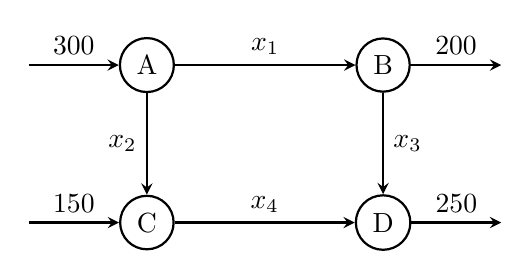
\begin{tikzpicture}[>=stealth,thick]
% Nodes
\node[circle,draw] (A) at (0,2) {A};
\node[circle,draw] (B) at (3,2) {B};
\node[circle,draw] (C) at (0,0) {C};
\node[circle,draw] (D) at (3,0) {D};

% External flows
\draw[->] (-1.5,2) -- (A) node[midway,above] {300};
\draw[->] (B) -- (4.5,2) node[midway,above] {200};
\draw[->] (D) -- (4.5,0) node[midway,above] {250};
\draw[->] (-1.5,0) -- (C) node[midway,above] {150};

% Internal flows
\draw[->] (A) -- (B) node[midway,above] {$x_1$};
\draw[->] (A) -- (C) node[midway,left] {$x_2$};
\draw[->] (B) -- (D) node[midway,right] {$x_3$};
\draw[->] (C) -- (D) node[midway,above] {$x_4$};
\end{tikzpicture}
\end{center}

Applying conservation of flow at each node:

\textbf{Node A:} $300 = x_1 + x_2$
\textbf{Node B:} $x_1 = 200 + x_3$  
\textbf{Node C:} $150 + x_2 = x_4$
\textbf{Node D:} $x_3 + x_4 = 250$

This gives us the system:
\begin{align}
x_1 + x_2 + 0x_3 + 0x_4 &= 300\\
x_1 + 0x_2 - x_3 + 0x_4 &= 200\\
0x_1 + x_2 + 0x_3 - x_4 &= -150\\
0x_1 + 0x_2 + x_3 + x_4 &= 250
\end{align}

Row reducing the augmented matrix:
$$\begin{amatrix}{rrrr|r}
1 & 1 & 0 & 0 & 300\\
1 & 0 & -1 & 0 & 200\\
0 & 1 & 0 & -1 & -150\\
0 & 0 & 1 & 1 & 250
\end{amatrix} \sim \begin{amatrix}{rrrr|r}
1 & 0 & 0 & 1 & 50\\
0 & 1 & 0 & -1 & -150\\
0 & 0 & 1 & 1 & 250\\
0 & 0 & 0 & 0 & 0
\end{amatrix}$$

Setting $x_4 = t$ (free variable):
\begin{align}
x_1 &= 50 - t\\
x_2 &= t - 150\\  
x_3 &= 250 - t\\
x_4 &= t
\end{align}

For physical feasibility, all flows must be non-negative:
$x_1 \geq 0 \Rightarrow t \leq 50$, $x_2 \geq 0 \Rightarrow t \geq 150$, $x_3 \geq 0 \Rightarrow t \leq 250$

Therefore $150 \leq t \leq 50$, which is impossible! This indicates the given external flows are incompatible with the network structure - the traffic demands cannot be satisfied.
\end{example}

\subsubsection{Electrical Networks}
Electrical circuit analysis relies on two fundamental laws that lead to systems of linear equations.
\begin{definition}[Kirchhoff's Laws]
\begin{enumerate}
\item \textbf{Kirchhoff's Current Law (KCL):} The sum of currents entering any node equals the sum of currents leaving that node
\item \textbf{Kirchhoff's Voltage Law (KVL):} The sum of voltage drops around any closed loop is zero
\end{enumerate}
\end{definition}
\begin{example}[DC Circuit Analysis]
Consider the circuit with three loops and resistors $R_1 = 2\Omega$, $R_2 = 4\Omega$, $R_3 = 1\Omega$, and voltage sources $V_1 = 12V$, $V_2 = 8V$.
Let $i_1$, $i_2$, $i_3$ be the loop currents (clockwise positive).
\textbf{Loop 1:} $2i_1 + 4(i_1 - i_2) = 12$
\textbf{Loop 2:} $4(i_2 - i_1) + 1(i_2 - i_3) = 0$  
\textbf{Loop 3:} $1(i_3 - i_2) = -8$
Simplifying:
\begin{align}
6i_1 - 4i_2 + 0i_3 &= 12\\
-4i_1 + 5i_2 - i_3 &= 0\\
0i_1 - i_2 + i_3 &= -8
\end{align}
Solving this system:
$$\begin{amatrix}{rrr|r}
6 & -4 & 0 & 12\\
-4 & 5 & -1 & 0\\
0 & -1 & 1 & -8
\end{amatrix} \sim \begin{amatrix}{rrr|r}
1 & 0 & 0 & 2\\
0 & 1 & 0 & 0\\
0 & 0 & 1 & -8
\end{amatrix}$$
Therefore: $i_1 = 2A$, $i_2 = 0A$, $i_3 = -8A$.
The actual branch currents can be found from the loop currents:
- Current through $R_1$: $i_1 = 2A$
- Current through $R_2$: $i_1 - i_2 = 2 - 0 = 2A$
- Current through $R_3$: $i_2 - i_3 = 0 - (-8) = 8A$
\end{example}

\subsubsection{Chemical Reactions}

Chemical equation balancing is a classic application of homogeneous linear systems, based on the principle of conservation of mass.

\begin{example}[Balancing Chemical Equations]
Balance the combustion reaction:
$$x_1 \text{C}_2\text{H}_6 + x_2 \text{O}_2 \rightarrow x_3 \text{CO}_2 + x_4 \text{H}_2\text{O}$$

Conservation of each element gives us:

\textbf{Carbon (C):} $2x_1 = x_3$
\textbf{Hydrogen (H):} $6x_1 = 2x_4$  
\textbf{Oxygen (O):} $2x_2 = 2x_3 + x_4$

This homogeneous system can be written as:
$$\begin{pmatrix}
2 & 0 & -1 & 0\\
6 & 0 & 0 & -2\\
0 & 2 & -2 & -1
\end{pmatrix}\begin{pmatrix} x_1 \\ x_2 \\ x_3 \\ x_4 \end{pmatrix} = \begin{pmatrix} 0 \\ 0 \\ 0 \end{pmatrix}$$

Row reducing:
$$\begin{amatrix}{rrrr|r}
2 & 0 & -1 & 0 & 0\\
6 & 0 & 0 & -2 & 0\\
0 & 2 & -2 & -1 & 0
\end{amatrix} \sim \begin{amatrix}{rrrr|r}
1 & 0 & 0 & -\frac{1}{3} & 0\\
0 & 1 & 0 & -\frac{7}{6} & 0\\
0 & 0 & 1 & -\frac{2}{3} & 0
\end{amatrix}$$

Setting $x_4 = t$:
$$x_1 = \frac{t}{3}, \quad x_2 = \frac{7t}{6}, \quad x_3 = \frac{2t}{3}, \quad x_4 = t$$

For integer coefficients, we choose $t = 6$:
$$x_1 = 2, \quad x_2 = 7, \quad x_3 = 4, \quad x_4 = 6$$

The balanced equation is:
$$2\text{C}_2\text{H}_6 + 7\text{O}_2 \rightarrow 4\text{CO}_2 + 6\text{H}_2\text{O}$$

\textbf{Verification:}
- Carbon: $2 \times 2 = 4$ on left, $4 \times 1 = 4$ on right \checkmark
- Hydrogen: $2 \times 6 = 12$ on left, $6 \times 2 = 12$ on right \checkmark  
- Oxygen: $7 \times 2 = 14$ on left, $4 \times 2 + 6 \times 1 = 14$ on right \checkmark
\end{example}

\begin{remark}
These applications demonstrate that linear systems are not merely abstract mathematical objects, but fundamental tools for modeling real-world phenomena. The systematic methods we've developed - matrix representations, elementary row operations, and Gaussian elimination - provide powerful computational tools for solving practical problems across diverse fields.
\end{remark}

This completes our comprehensive study of systems of linear equations. We have established the theoretical foundations, developed systematic solution methods, and explored practical applications. These concepts will serve as the cornerstone for our continued journey through linear algebra.

\newpage
% Topic 2: Matrix Algebra
\section{Matrix Algebra}

Matrices are rectangular arrays of numbers that serve as one of the most powerful tools in mathematics and its applications. They provide a compact way to represent and manipulate linear transformations, systems of equations, and countless other mathematical objects. This chapter develops the algebraic structure of matrices, establishing the rules and properties that govern matrix operations.

% =======================
% Section 2.1: Matrix Basics
% =======================
\subsection{Matrix Basics}

\subsubsection{Matrix Addition and Scalar Multiplication}

\begin{definition}[Matrix]
An $m \times n$ \textbf{matrix} is a rectangular array of real numbers arranged in $m$ rows and $n$ columns:
$$\mat{A} = \begin{pmatrix}
a_{11} & a_{12} & \cdots & a_{1n}\\
a_{21} & a_{22} & \cdots & a_{2n}\\
\vdots & \vdots & \ddots & \vdots\\
a_{m1} & a_{m2} & \cdots & a_{mn}
\end{pmatrix}$$
The number $a_{ij}$ is called the \textbf{$(i,j)$-entry} of $\mat{A}$, located in the $i$-th row and $j$-th column.
\end{definition}

\begin{notation}
We denote the set of all $m \times n$ matrices with real entries as $\mathbb{R}^{m \times n}$. When the dimensions are clear from context, we may write $\mat{A} = (a_{ij})$ to indicate that $\mat{A}$ has entries $a_{ij}$.
\end{notation}

\begin{remark}
The double subscript notation is crucial for matrix algebra. The first index always refers to the row, the second to the column. This convention, while arbitrary, is universally adopted and must be followed consistently.
\end{remark}

\begin{definition}[Matrix Equality]
Two matrices $\mat{A} = (a_{ij})$ and $\mat{B} = (b_{ij})$ are \textbf{equal} if:
\begin{enumerate}
\item They have the same dimensions ($m \times n$)
\item $a_{ij} = b_{ij}$ for all $i = 1, 2, \ldots, m$ and $j = 1, 2, \ldots, n$
\end{enumerate}
\end{definition}

Now we define the fundamental operations on matrices:

\begin{definition}[Matrix Addition]
If $\mat{A} = (a_{ij})$ and $\mat{B} = (b_{ij})$ are both $m \times n$ matrices, then their \textbf{sum} $\mat{A} + \mat{B}$ is the $m \times n$ matrix whose $(i,j)$-entry is $a_{ij} + b_{ij}$:
$$(\mat{A} + \mat{B})_{ij} = a_{ij} + b_{ij}$$
\end{definition}

\begin{remark}
Matrix addition is only defined for matrices of the same size. We cannot add a $2 \times 3$ matrix to a $3 \times 2$ matrix, even though both have six entries. The structural arrangement matters fundamentally.
\end{remark}

\begin{definition}[Scalar Multiplication]
If $\mat{A} = (a_{ij})$ is an $m \times n$ matrix and $c$ is a real number (scalar), then the \textbf{scalar multiple} $c\mat{A}$ is the $m \times n$ matrix whose $(i,j)$-entry is $ca_{ij}$:
$$(c\mat{A})_{ij} = ca_{ij}$$
\end{definition}

\begin{example}[Basic Matrix Operations]
Let $\mat{A} = \begin{pmatrix} 2 & -1 & 3 \\ 0 & 4 & -2 \end{pmatrix}$ and $\mat{B} = \begin{pmatrix} 1 & 5 & -1 \\ 3 & -2 & 7 \end{pmatrix}$.

\textbf{Matrix Addition:}
$$\mat{A} + \mat{B} = \begin{pmatrix} 2+1 & -1+5 & 3+(-1) \\ 0+3 & 4+(-2) & -2+7 \end{pmatrix} = \begin{pmatrix} 3 & 4 & 2 \\ 3 & 2 & 5 \end{pmatrix}$$

\textbf{Scalar Multiplication:}
$$3\mat{A} = \begin{pmatrix} 3 \cdot 2 & 3 \cdot (-1) & 3 \cdot 3 \\ 3 \cdot 0 & 3 \cdot 4 & 3 \cdot (-2) \end{pmatrix} = \begin{pmatrix} 6 & -3 & 9 \\ 0 & 12 & -6 \end{pmatrix}$$

\textbf{Combined Operations:}
$$2\mat{A} - 3\mat{B} = \begin{pmatrix} 4 & -2 & 6 \\ 0 & 8 & -4 \end{pmatrix} - \begin{pmatrix} 3 & 15 & -3 \\ 9 & -6 & 21 \end{pmatrix} = \begin{pmatrix} 1 & -17 & 9 \\ -9 & 14 & -25 \end{pmatrix}$$
\end{example}

The algebraic properties of matrix addition and scalar multiplication mirror those of real number arithmetic:

\begin{theorem}[Properties of Matrix Addition and Scalar Multiplication]
Let $\mat{A}$, $\mat{B}$, and $\mat{C}$ be $m \times n$ matrices, and let $r$ and $s$ be scalars. Then:

\textbf{Addition Properties:}
\begin{enumerate}
\item $\mat{A} + \mat{B} = \mat{B} + \mat{A}$ (commutativity)
\item $(\mat{A} + \mat{B}) + \mat{C} = \mat{A} + (\mat{B} + \mat{C})$ (associativity)
\item $\mat{A} + \mat{0} = \mat{A}$ (additive identity, where $\mat{0}$ is the zero matrix)
\item $\mat{A} + (-\mat{A}) = \mat{0}$ (additive inverse)
\end{enumerate}

\textbf{Scalar Multiplication Properties:}
\begin{enumerate}[resume]
\item $r(\mat{A} + \mat{B}) = r\mat{A} + r\mat{B}$ (distributivity over matrix addition)
\item $(r + s)\mat{A} = r\mat{A} + s\mat{A}$ (distributivity over scalar addition)
\item $r(s\mat{A}) = (rs)\mat{A}$ (associativity of scalar multiplication)
\item $1 \cdot \mat{A} = \mat{A}$ (scalar multiplicative identity)
\end{enumerate}
\end{theorem}

\begin{proof}
We prove property (1) and (5); the others follow similarly.

\textbf{Property (1):} For any $i,j$:
$$(\mat{A} + \mat{B})_{ij} = a_{ij} + b_{ij} = b_{ij} + a_{ij} = (\mat{B} + \mat{A})_{ij}$$
Since this holds for all entries, $\mat{A} + \mat{B} = \mat{B} + \mat{A}$.

\textbf{Property (5):} For any $i,j$:
$$(r(\mat{A} + \mat{B}))_{ij} = r(\mat{A} + \mat{B})_{ij} = r(a_{ij} + b_{ij}) = ra_{ij} + rb_{ij} = (r\mat{A})_{ij} + (r\mat{B})_{ij} = (r\mat{A} + r\mat{B})_{ij}$$
\end{proof}

\begin{definition}[Zero Matrix]
The $m \times n$ \textbf{zero matrix}, denoted $\mat{0}$ or $\mat{0}_{m \times n}$, is the matrix whose entries are all zero.
\end{definition}

\begin{definition}[Negative of a Matrix]
The \textbf{negative} of a matrix $\mat{A}$, denoted $-\mat{A}$, is the matrix $(-1)\mat{A}$.
\end{definition}

\begin{keyidea}
These properties establish that the set of all $m \times n$ matrices, together with matrix addition and scalar multiplication, forms a \textbf{vector space}. This is our first encounter with this fundamental algebraic structure, which will be explored in detail in later chapters.
\end{keyidea}

\subsubsection{Transpose and Symmetry}

\begin{definition}[Transpose]
The \textbf{transpose} of an $m \times n$ matrix $\mat{A} = (a_{ij})$ is the $n \times m$ matrix $\mat{A}^{\trans}$ whose $(i,j)$-entry is $a_{ji}$:
$$(\mat{A}^{\trans})_{ij} = a_{ji}$$
In other words, the rows of $\mat{A}$ become the columns of $\mat{A}^{\trans}$, and vice versa.
\end{definition}

\begin{example}[Computing Transposes]
\begin{align}
\text{If } \mat{A} &= \begin{pmatrix} 1 & 2 & 3 \\ 4 & 5 & 6 \end{pmatrix}, \text{ then } \mat{A}^{\trans} = \begin{pmatrix} 1 & 4 \\ 2 & 5 \\ 3 & 6 \end{pmatrix}\\[0.5em]
\text{If } \mat{B} &= \begin{pmatrix} 2 \\ -1 \\ 3 \end{pmatrix}, \text{ then } \mat{B}^{\trans} = \begin{pmatrix} 2 & -1 & 3 \end{pmatrix}\\[0.5em]
\text{If } \mat{C} &= \begin{pmatrix} 5 \end{pmatrix}, \text{ then } \mat{C}^{\trans} = \begin{pmatrix} 5 \end{pmatrix}
\end{align}
\end{example}

\begin{theorem}[Properties of Transpose]
Let $\mat{A}$ and $\mat{B}$ be matrices of appropriate sizes, and let $r$ be a scalar. Then:
\begin{enumerate}
\item $(\mat{A}^{\trans})^{\trans} = \mat{A}$
\item $(\mat{A} + \mat{B})^{\trans} = \mat{A}^{\trans} + \mat{B}^{\trans}$
\item $(r\mat{A})^{\trans} = r\mat{A}^{\trans}$
\item $(\mat{A}\mat{B})^{\trans} = \mat{B}^{\trans}\mat{A}^{\trans}$ (when the product $\mat{A}\mat{B}$ is defined)
\end{enumerate}
\end{theorem}

\begin{proof}
\textbf{Property (1):} For any $i,j$:
$$((\mat{A}^{\trans})^{\trans})_{ij} = (\mat{A}^{\trans})_{ji} = a_{ij}$$
Thus $(\mat{A}^{\trans})^{\trans} = \mat{A}$.

\textbf{Property (2):} For any $i,j$:
$$((\mat{A} + \mat{B})^{\trans})_{ij} = (\mat{A} + \mat{B})_{ji} = a_{ji} + b_{ji} = (\mat{A}^{\trans})_{ij} + (\mat{B}^{\trans})_{ij}$$

\textbf{Property (3):} For any $i,j$:
$$((r\mat{A})^{\trans})_{ij} = (r\mat{A})_{ji} = ra_{ji} = r(\mat{A}^{\trans})_{ij}$$

Property (4) will be proved after we define matrix multiplication.
\end{proof}

\begin{definition}[Symmetric Matrix]
A square matrix $\mat{A}$ is \textbf{symmetric} if $\mat{A} = \mat{A}^{\trans}$, i.e., $a_{ij} = a_{ji}$ for all $i,j$.
\end{definition}

\begin{definition}[Skew-Symmetric Matrix]
A square matrix $\mat{A}$ is \textbf{skew-symmetric} (or \textbf{antisymmetric}) if $\mat{A} = -\mat{A}^{\trans}$, i.e., $a_{ij} = -a_{ji}$ for all $i,j$.
\end{definition}

\begin{example}[Symmetric and Skew-Symmetric Matrices]
\textbf{Symmetric matrix:}
$$\mat{A} = \begin{pmatrix} 1 & 2 & 3 \\ 2 & 5 & -1 \\ 3 & -1 & 0 \end{pmatrix}$$
Note that $a_{12} = a_{21} = 2$, $a_{13} = a_{31} = 3$, and $a_{23} = a_{32} = -1$.

\textbf{Skew-symmetric matrix:}
$$\mat{B} = \begin{pmatrix} 0 & 2 & -3 \\ -2 & 0 & 1 \\ 3 & -1 & 0 \end{pmatrix}$$
Note that the diagonal entries are all zero (since $a_{ii} = -a_{ii}$ implies $a_{ii} = 0$), and off-diagonal entries satisfy $a_{ij} = -a_{ji}$.
\end{example}

\begin{theorem}[Decomposition into Symmetric and Skew-Symmetric Parts]
Every square matrix $\mat{A}$ can be uniquely written as the sum of a symmetric matrix and a skew-symmetric matrix:
$$\mat{A} = \frac{1}{2}(\mat{A} + \mat{A}^{\trans}) + \frac{1}{2}(\mat{A} - \mat{A}^{\trans})$$
where $\frac{1}{2}(\mat{A} + \mat{A}^{\trans})$ is symmetric and $\frac{1}{2}(\mat{A} - \mat{A}^{\trans})$ is skew-symmetric.
\end{theorem}

\begin{proof}
Let $\mat{S} = \frac{1}{2}(\mat{A} + \mat{A}^{\trans})$ and $\mat{K} = \frac{1}{2}(\mat{A} - \mat{A}^{\trans})$.

\textbf{Verification that $\mat{S}$ is symmetric:}
$$\mat{S}^{\trans} = \left(\frac{1}{2}(\mat{A} + \mat{A}^{\trans})\right)^{\trans} = \frac{1}{2}(\mat{A}^{\trans} + (\mat{A}^{\trans})^{\trans}) = \frac{1}{2}(\mat{A}^{\trans} + \mat{A}) = \mat{S}$$

\textbf{Verification that $\mat{K}$ is skew-symmetric:}
$$\mat{K}^{\trans} = \left(\frac{1}{2}(\mat{A} - \mat{A}^{\trans})\right)^{\trans} = \frac{1}{2}(\mat{A}^{\trans} - (\mat{A}^{\trans})^{\trans}) = \frac{1}{2}(\mat{A}^{\trans} - \mat{A}) = -\mat{K}$$

\textbf{Verification of the decomposition:}
$$\mat{S} + \mat{K} = \frac{1}{2}(\mat{A} + \mat{A}^{\trans}) + \frac{1}{2}(\mat{A} - \mat{A}^{\trans}) = \frac{1}{2}(2\mat{A}) = \mat{A}$$

\textbf{Uniqueness:} If $\mat{A} = \mat{S}_1 + \mat{K}_1 = \mat{S}_2 + \mat{K}_2$ where $\mat{S}_1, \mat{S}_2$ are symmetric and $\mat{K}_1, \mat{K}_2$ are skew-symmetric, then:
$$\mat{S}_1 - \mat{S}_2 = \mat{K}_2 - \mat{K}_1$$
The left side is symmetric, the right side is skew-symmetric. The only matrix that is both symmetric and skew-symmetric is the zero matrix, so $\mat{S}_1 = \mat{S}_2$ and $\mat{K}_1 = \mat{K}_2$.
\end{proof}

% =======================
% Section 2.2: Matrix-Vector Multiplication
% =======================
\subsection{Matrix-Vector Multiplication}

Before tackling general matrix multiplication, we first study the multiplication of a matrix by a vector, which provides essential intuition and forms the foundation for more complex operations.

\subsubsection{Dot Product Interpretation}

\begin{definition}[Dot Product]
The \textbf{dot product} (or \textbf{inner product}) of two vectors $\vect{u} = \begin{pmatrix} u_1 \\ u_2 \\ \vdots \\ u_n \end{pmatrix}$ and $\vect{v} = \begin{pmatrix} v_1 \\ v_2 \\ \vdots \\ v_n \end{pmatrix}$ in $\RR^n$ is:
$$\vect{u} \cdot \vect{v} = u_1v_1 + u_2v_2 + \cdots + u_nv_n = \sum_{i=1}^n u_iv_i$$
\end{definition}

\begin{definition}[Matrix-Vector Product (Row Perspective)]
If $\mat{A}$ is an $m \times n$ matrix and $\vect{x}$ is a vector in $\RR^n$, then the \textbf{product} $\mat{A}\vect{x}$ is the vector in $\RR^m$ whose $i$-th entry is the dot product of the $i$-th row of $\mat{A}$ with $\vect{x}$:
$$(\mat{A}\vect{x})_i = \text{row}_i(\mat{A}) \cdot \vect{x} = \sum_{j=1}^n a_{ij}x_j$$
\end{definition}

\begin{example}[Matrix-Vector Multiplication]
$$\begin{pmatrix} 2 & -1 & 3 \\ 0 & 4 & -2 \\ 1 & 1 & 1 \end{pmatrix} \begin{pmatrix} 1 \\ 2 \\ -1 \end{pmatrix} = \begin{pmatrix} 2(1) + (-1)(2) + 3(-1) \\ 0(1) + 4(2) + (-2)(-1) \\ 1(1) + 1(2) + 1(-1) \end{pmatrix} = \begin{pmatrix} -3 \\ 10 \\ 2 \end{pmatrix}$$

\textbf{Detailed computation:}
\begin{align}
\text{First entry:} \quad &(2, -1, 3) \cdot (1, 2, -1) = 2 - 2 - 3 = -3\\
\text{Second entry:} \quad &(0, 4, -2) \cdot (1, 2, -1) = 0 + 8 + 2 = 10\\
\text{Third entry:} \quad &(1, 1, 1) \cdot (1, 2, -1) = 1 + 2 - 1 = 2
\end{align}
\end{example}

\begin{remark}
The matrix-vector product $\mat{A}\vect{x}$ is only defined when the number of columns of $\mat{A}$ equals the number of entries in $\vect{x}$. The result is a vector with the same number of entries as the number of rows of $\mat{A}$.
\end{remark}

There is an alternative, equally important way to view matrix-vector multiplication:

\begin{theorem}[Column Interpretation of Matrix-Vector Product]
If $\mat{A} = [\vect{a}_1 \mid \vect{a}_2 \mid \cdots \mid \vect{a}_n]$ where $\vect{a}_j$ denotes the $j$-th column of $\mat{A}$, and $\vect{x} = \begin{pmatrix} x_1 \\ x_2 \\ \vdots \\ x_n \end{pmatrix}$, then:
$$\mat{A}\vect{x} = x_1\vect{a}_1 + x_2\vect{a}_2 + \cdots + x_n\vect{a}_n$$
\end{theorem}

\begin{proof}
Let's compute the $i$-th entry of both sides:

\textbf{Left side:} $(\mat{A}\vect{x})_i = \sum_{j=1}^n a_{ij}x_j$

\textbf{Right side:} $(x_1\vect{a}_1 + x_2\vect{a}_2 + \cdots + x_n\vect{a}_n)_i = x_1(\vect{a}_1)_i + x_2(\vect{a}_2)_i + \cdots + x_n(\vect{a}_n)_i = x_1a_{i1} + x_2a_{i2} + \cdots + x_na_{in} = \sum_{j=1}^n a_{ij}x_j$

Since the $i$-th entries are equal for all $i$, the vectors are equal.
\end{proof}

\begin{example}[Column Interpretation]
Using the same example as before:
$$\begin{pmatrix} 2 & -1 & 3 \\ 0 & 4 & -2 \\ 1 & 1 & 1 \end{pmatrix} \begin{pmatrix} 1 \\ 2 \\ -1 \end{pmatrix} = 1\begin{pmatrix} 2 \\ 0 \\ 1 \end{pmatrix} + 2\begin{pmatrix} -1 \\ 4 \\ 1 \end{pmatrix} + (-1)\begin{pmatrix} 3 \\ -2 \\ 1 \end{pmatrix}$$

$$= \begin{pmatrix} 2 \\ 0 \\ 1 \end{pmatrix} + \begin{pmatrix} -2 \\ 8 \\ 2 \end{pmatrix} + \begin{pmatrix} -3 \\ 2 \\ -1 \end{pmatrix} = \begin{pmatrix} -3 \\ 10 \\ 2 \end{pmatrix}$$
\end{example}

\begin{keyidea}
The column interpretation reveals that $\mat{A}\vect{x}$ is a \textbf{linear combination} of the columns of $\mat{A}$, with coefficients given by the entries of $\vect{x}$. This perspective is fundamental to understanding the geometric meaning of matrix transformations.
\end{keyidea}

\subsubsection{Matrices as Linear Transformations}

Matrix-vector multiplication can be viewed as a function that maps vectors to vectors. This viewpoint opens up rich geometric interpretations.

\begin{definition}[Matrix Transformation]
For an $m \times n$ matrix $\mat{A}$, the \textbf{matrix transformation} $T_{\mat{A}}: \RR^n \to \RR^m$ is defined by:
$$T_{\mat{A}}(\vect{x}) = \mat{A}\vect{x}$$
\end{definition}

\begin{theorem}[Linearity of Matrix Transformations]
Every matrix transformation is linear, meaning:
\begin{enumerate}
\item $T_{\mat{A}}(\vect{u} + \vect{v}) = T_{\mat{A}}(\vect{u}) + T_{\mat{A}}(\vect{v})$ for all $\vect{u}, \vect{v} \in \RR^n$
\item $T_{\mat{A}}(c\vect{u}) = cT_{\mat{A}}(\vect{u})$ for all $\vect{u} \in \RR^n$ and scalars $c$
\end{enumerate}
Equivalently, $T_{\mat{A}}(c\vect{u} + d\vect{v}) = cT_{\mat{A}}(\vect{u}) + dT_{\mat{A}}(\vect{v})$ for all vectors $\vect{u}, \vect{v}$ and scalars $c, d$.
\end{theorem}

\begin{proof}
\textbf{Property 1:} Using the $i$-th entry:
\begin{align}
(T_{\mat{A}}(\vect{u} + \vect{v}))_i &= (\mat{A}(\vect{u} + \vect{v}))_i = \sum_{j=1}^n a_{ij}(u_j + v_j)\\
&= \sum_{j=1}^n a_{ij}u_j + \sum_{j=1}^n a_{ij}v_j = (\mat{A}\vect{u})_i + (\mat{A}\vect{v})_i\\
&= (T_{\mat{A}}(\vect{u}) + T_{\mat{A}}(\vect{v}))_i
\end{align}

\textbf{Property 2:} Similarly:
$$(T_{\mat{A}}(c\vect{u}))_i = (\mat{A}(c\vect{u}))_i = \sum_{j=1}^n a_{ij}(cu_j) = c\sum_{j=1}^n a_{ij}u_j = c(\mat{A}\vect{u})_i = (cT_{\mat{A}}(\vect{u}))_i$$
\end{proof}

Let's explore some important geometric transformations in $\RR^2$:

\begin{example}[Rotation Transformation]
The matrix $\mat{R}_{\theta} = \begin{pmatrix} \cos\theta & -\sin\theta \\ \sin\theta & \cos\theta \end{pmatrix}$ represents counterclockwise rotation by angle $\theta$ about the origin.

\textbf{Verification:} Consider the standard basis vectors:
$$\mat{R}_{\theta}\begin{pmatrix} 1 \\ 0 \end{pmatrix} = \begin{pmatrix} \cos\theta \\ \sin\theta \end{pmatrix}, \quad \mat{R}_{\theta}\begin{pmatrix} 0 \\ 1 \end{pmatrix} = \begin{pmatrix} -\sin\theta \\ \cos\theta \end{pmatrix}$$

These are indeed the results of rotating $(1,0)$ and $(0,1)$ by angle $\theta$.

\textbf{Specific example:} Rotation by $90°$ ($\theta = \pi/2$):
$$\mat{R}_{\pi/2} = \begin{pmatrix} 0 & -1 \\ 1 & 0 \end{pmatrix}$$

Check: $\begin{pmatrix} 0 & -1 \\ 1 & 0 \end{pmatrix}\begin{pmatrix} 3 \\ 2 \end{pmatrix} = \begin{pmatrix} -2 \\ 3 \end{pmatrix}$

The point $(3,2)$ is rotated to $(-2,3)$, which is indeed a $90°$ counterclockwise rotation.
\end{example}

\begin{example}[Reflection Transformation]
The matrix $\mat{F} = \begin{pmatrix} 1 & 0 \\ 0 & -1 \end{pmatrix}$ represents reflection across the $x$-axis.

$$\mat{F}\begin{pmatrix} x \\ y \end{pmatrix} = \begin{pmatrix} x \\ -y \end{pmatrix}$$

The $x$-coordinate remains unchanged, while the $y$-coordinate is negated, which is exactly what reflection across the $x$-axis should do.
\end{example}

\begin{example}[Scaling Transformation]
The matrix $\mat{S} = \begin{pmatrix} a & 0 \\ 0 & b \end{pmatrix}$ represents scaling by factor $a$ in the $x$-direction and factor $b$ in the $y$-direction.

$$\mat{S}\begin{pmatrix} x \\ y \end{pmatrix} = \begin{pmatrix} ax \\ by \end{pmatrix}$$

When $a = b$, this is uniform scaling. When $a \neq b$, the transformation stretches or compresses differently in each direction.
\end{example}

\begin{example}[Shear Transformation]
The matrix $\mat{H} = \begin{pmatrix} 1 & k \\ 0 & 1 \end{pmatrix}$ represents horizontal shear with parameter $k$.

$$\mat{H}\begin{pmatrix} x \\ y \end{pmatrix} = \begin{pmatrix} x + ky \\ y \end{pmatrix}$$

Points are shifted horizontally by an amount proportional to their $y$-coordinate, while the $y$-coordinate remains unchanged.
\end{example}

% =======================
% Section 2.3: Matrix Multiplication
% =======================
\subsection{Matrix Multiplication}

Building on matrix-vector multiplication, we now define the multiplication of two matrices. This operation, while initially seeming complex, has a natural motivation and profound applications.

\begin{definition}[Matrix Multiplication]
If $\mat{A}$ is an $m \times p$ matrix and $\mat{B}$ is a $p \times n$ matrix, then the \textbf{product} $\mat{A}\mat{B}$ is the $m \times n$ matrix whose $(i,j)$-entry is:
$$(\mat{A}\mat{B})_{ij} = \sum_{k=1}^p a_{ik}b_{kj}$$
This is the dot product of the $i$-th row of $\mat{A}$ with the $j$-th column of $\mat{B}$.
\end{definition}

\begin{remark}
The product $\mat{A}\mat{B}$ is only defined when the number of columns of $\mat{A}$ equals the number of rows of $\mat{B}$. The resulting matrix has dimensions determined by the outer dimensions: if $\mat{A}$ is $m \times p$ and $\mat{B}$ is $p \times n$, then $\mat{A}\mat{B}$ is $m \times n$.
\end{remark}

\begin{example}[Matrix Multiplication Computation]
$$\begin{pmatrix} 1 & 2 \\ 3 & 4 \\ 5 & 6 \end{pmatrix} \begin{pmatrix} 7 & 8 & 9 \\ 10 & 11 & 12 \end{pmatrix}$$

\textbf{Step-by-step computation:}
\begin{align}
(1,1)\text{-entry:} \quad &(1, 2) \cdot (7, 10) = 1 \cdot 7 + 2 \cdot 10 = 27\\
(1,2)\text{-entry:} \quad &(1, 2) \cdot (8, 11) = 1 \cdot 8 + 2 \cdot 11 = 30\\
(1,3)\text{-entry:} \quad &(1, 2) \cdot (9, 12) = 1 \cdot 9 + 2 \cdot 12 = 33\\
(2,1)\text{-entry:} \quad &(3, 4) \cdot (7, 10) = 3 \cdot 7 + 4 \cdot 10 = 61\\
(2,2)\text{-entry:} \quad &(3, 4) \cdot (8, 11) = 3 \cdot 8 + 4 \cdot 11 = 68\\
(2,3)\text{-entry:} \quad &(3, 4) \cdot (9, 12) = 3 \cdot 9 + 4 \cdot 12 = 75\\
(3,1)\text{-entry:} \quad &(5, 6) \cdot (7, 10) = 5 \cdot 7 + 6 \cdot 10 = 95\\
(3,2)\text{-entry:} \quad &(5, 6) \cdot (8, 11) = 5 \cdot 8 + 6 \cdot 11 = 106\\
(3,3)\text{-entry:} \quad &(5, 6) \cdot (9, 12) = 5 \cdot 9 + 6 \cdot 12 = 117
\end{align}

\textbf{Result:}
$$\begin{pmatrix} 1 & 2 \\ 3 & 4 \\ 5 & 6 \end{pmatrix} \begin{pmatrix} 7 & 8 & 9 \\ 10 & 11 & 12 \end{pmatrix} = \begin{pmatrix} 27 & 30 & 33 \\ 61 & 68 & 75 \\ 95 & 106 & 117 \end{pmatrix}$$
\end{example}

\subsubsection{Column Interpretation}

Just as with matrix-vector multiplication, there's an insightful column interpretation:

\begin{theorem}[Column Interpretation of Matrix Multiplication]
If $\mat{A}$ is $m \times p$ and $\mat{B} = [\vect{b}_1 \mid \vect{b}_2 \mid \cdots \mid \vect{b}_n]$ where $\vect{b}_j$ is the $j$-th column of $\mat{B}$, then:
$$\mat{A}\mat{B} = [\mat{A}\vect{b}_1 \mid \mat{A}\vect{b}_2 \mid \cdots \mid \mat{A}\vect{b}_n]$$
In other words, the $j$-th column of $\mat{A}\mat{B}$ is $\mat{A}$ times the $j$-th column of $\mat{B}$.
\end{theorem}

\begin{proof}
The $j$-th column of $\mat{A}\mat{B}$ has entries $(\mat{A}\mat{B})_{ij}$ for $i = 1, 2, \ldots, m$. By definition:
$$(\mat{A}\mat{B})_{ij} = \sum_{k=1}^p a_{ik}b_{kj}$$

On the other hand, $(\mat{A}\vect{b}_j)_i = \sum_{k=1}^p a_{ik}(\vect{b}_j)_k = \sum_{k=1}^p a_{ik}b_{kj}$.

Since these expressions are equal, the $j$-th column of $\mat{A}\mat{B}$ equals $\mat{A}\vect{b}_j$.
\end{proof}

\begin{example}[Using Column Interpretation]
Let's verify our previous example using the column interpretation:
$$\mat{A} = \begin{pmatrix} 1 & 2 \\ 3 & 4 \\ 5 & 6 \end{pmatrix}, \quad \mat{B} = \begin{pmatrix} 7 & 8 & 9 \\ 10 & 11 & 12 \end{pmatrix}$$

\textbf{First column of $\mat{A}\mat{B}$:}
$$\mat{A}\begin{pmatrix} 7 \\ 10 \end{pmatrix} = \begin{pmatrix} 1 & 2 \\ 3 & 4 \\ 5 & 6 \end{pmatrix}\begin{pmatrix} 7 \\ 10 \end{pmatrix} = \begin{pmatrix} 27 \\ 61 \\ 95 \end{pmatrix}$$

\textbf{Second column of $\mat{A}\mat{B}$:}
$$\mat{A}\begin{pmatrix} 8 \\ 11 \end{pmatrix} = \begin{pmatrix} 1 & 2 \\ 3 & 4 \\ 5 & 6 \end{pmatrix}\begin{pmatrix} 8 \\ 11 \end{pmatrix} = \begin{pmatrix} 30 \\ 68 \\ 106 \end{pmatrix}$$

\textbf{Third column of $\mat{A}\mat{B}$:}
$$\mat{A}\begin{pmatrix} 9 \\ 12 \end{pmatrix} = \begin{pmatrix} 1 & 2 \\ 3 & 4 \\ 5 & 6 \end{pmatrix}\begin{pmatrix} 9 \\ 12 \end{pmatrix} = \begin{pmatrix} 33 \\ 75 \\ 117 \end{pmatrix}$$

This confirms our previous result.
\end{example}

\subsubsection{Associativity Proof}

One of the most important properties of matrix multiplication is associativity. Although the proof is computational, it's essential for understanding why we can write expressions like $\mat{A}\mat{B}\mat{C}$ without ambiguity.

\begin{theorem}[Associativity of Matrix Multiplication]
If $\mat{A}$, $\mat{B}$, and $\mat{C}$ are matrices such that the products $\mat{A}\mat{B}$ and $\mat{B}\mat{C}$ are defined, then:
$$(\mat{A}\mat{B})\mat{C} = \mat{A}(\mat{B}\mat{C})$$
\end{theorem}

\begin{proof}
Suppose $\mat{A}$ is $m \times p$, $\mat{B}$ is $p \times q$, and $\mat{C}$ is $q \times n$. We need to show that the $(i,j)$-entries of both sides are equal.

\textbf{Left side} $((\mat{A}\mat{B})\mat{C})_{ij}$:
$$= \sum_{k=1}^q (\mat{A}\mat{B})_{ik} \cdot c_{kj} = \sum_{k=1}^q \left(\sum_{\ell=1}^p a_{i\ell}b_{\ell k}\right) c_{kj} = \sum_{k=1}^q \sum_{\ell=1}^p a_{i\ell}b_{\ell k}c_{kj}$$

\textbf{Right side} $(\mat{A}(\mat{B}\mat{C}))_{ij}$:
$$= \sum_{\ell=1}^p a_{i\ell} \cdot (\mat{B}\mat{C})_{\ell j} = \sum_{\ell=1}^p a_{i\ell} \left(\sum_{k=1}^q b_{\ell k}c_{kj}\right) = \sum_{\ell=1}^p \sum_{k=1}^q a_{i\ell}b_{\ell k}c_{kj}$$

Since addition of real numbers is commutative and associative, we can rearrange the double sum:
$$\sum_{k=1}^q \sum_{\ell=1}^p a_{i\ell}b_{\ell k}c_{kj} = \sum_{\ell=1}^p \sum_{k=1}^q a_{i\ell}b_{\ell k}c_{kj}$$

Therefore, the $(i,j)$-entries are equal, proving associativity.
\end{proof}

\begin{remark}
This proof shows that associativity follows from the associativity and commutativity of real number addition and multiplication. The rearrangement of the double sum is the key insight.
\end{remark}

\begin{theorem}[Properties of Matrix Multiplication]
Let $\mat{A}$, $\mat{B}$, and $\mat{C}$ be matrices of appropriate sizes, and let $r$ be a scalar. Then:
\begin{enumerate}
\item $\mat{A}(\mat{B}\mat{C}) = (\mat{A}\mat{B})\mat{C}$ (associativity)
\item $\mat{A}(\mat{B} + \mat{C}) = \mat{A}\mat{B} + \mat{A}\mat{C}$ (left distributivity)
\item $(\mat{B} + \mat{C})\mat{A} = \mat{B}\mat{A} + \mat{C}\mat{A}$ (right distributivity)
\item $(r\mat{A})\mat{B} = r(\mat{A}\mat{B}) = \mat{A}(r\mat{B})$ (scalar associativity)
\item $\mat{A}\mat{0} = \mat{0}$ and $\mat{0}\mat{A} = \mat{0}$ (multiplication by zero)
\end{enumerate}
\end{theorem}

\begin{example}[Matrix Multiplication is Not Commutative]
In general, $\mat{A}\mat{B} \neq \mat{B}\mat{A}$. Consider:
$$\mat{A} = \begin{pmatrix} 1 & 2 \\ 3 & 4 \end{pmatrix}, \quad \mat{B} = \begin{pmatrix} 0 & 1 \\ 0 & 0 \end{pmatrix}$$

$$\mat{A}\mat{B} = \begin{pmatrix} 1 & 2 \\ 3 & 4 \end{pmatrix}\begin{pmatrix} 0 & 1 \\ 0 & 0 \end{pmatrix} = \begin{pmatrix} 0 & 1 \\ 0 & 3 \end{pmatrix}$$

$$\mat{B}\mat{A} = \begin{pmatrix} 0 & 1 \\ 0 & 0 \end{pmatrix}\begin{pmatrix} 1 & 2 \\ 3 & 4 \end{pmatrix} = \begin{pmatrix} 3 & 4 \\ 0 & 0 \end{pmatrix}$$

Clearly $\mat{A}\mat{B} \neq \mat{B}\mat{A}$.
\end{example}

\subsubsection{Directed Graphs and Composition of Maps}

Matrix multiplication has elegant interpretations in terms of directed graphs and function composition.

\begin{definition}[Adjacency Matrix]
For a directed graph with $n$ vertices, the \textbf{adjacency matrix} $\mat{A}$ is the $n \times n$ matrix where $a_{ij} = 1$ if there is an edge from vertex $i$ to vertex $j$, and $a_{ij} = 0$ otherwise.
\end{definition}

\begin{theorem}[Powers of Adjacency Matrix]
If $\mat{A}$ is the adjacency matrix of a directed graph, then $(\mat{A}^k)_{ij}$ equals the number of paths of length $k$ from vertex $i$ to vertex $j$.
\end{theorem}

\begin{proof}
We use induction on $k$.

\textbf{Base case ($k = 1$):} $(\mat{A}^1)_{ij} = a_{ij}$ is 1 if there's a direct edge from $i$ to $j$ (a path of length 1), and 0 otherwise.

\textbf{Inductive step:} Assume the statement holds for paths of length $k$. For paths of length $k+1$:
$$(\mat{A}^{k+1})_{ij} = (\mat{A}^k \mat{A})_{ij} = \sum_{\ell=1}^n (\mat{A}^k)_{i\ell} \cdot a_{\ell j}$$

By the inductive hypothesis, $(\mat{A}^k)_{i\ell}$ counts paths of length $k$ from $i$ to $\ell$. The term $a_{\ell j}$ is 1 if there's an edge from $\ell$ to $j$, and 0 otherwise. Therefore, $(\mat{A}^k)_{i\ell} \cdot a_{\ell j}$ counts paths of length $k+1$ from $i$ to $j$ that pass through $\ell$. Summing over all possible intermediate vertices $\ell$ gives the total number of paths of length $k+1$ from $i$ to $j$.
\end{proof}

\begin{example}[Graph Paths]
Consider the directed graph with adjacency matrix:
$$\mat{A} = \begin{pmatrix} 0 & 1 & 1 \\ 1 & 0 & 1 \\ 0 & 1 & 0 \end{pmatrix}$$

This represents a graph where:
- Vertex 1 connects to vertices 2 and 3
- Vertex 2 connects to vertices 1 and 3  
- Vertex 3 connects to vertex 2

Let's compute $\mat{A}^2$:
$$\mat{A}^2 = \begin{pmatrix} 0 & 1 & 1 \\ 1 & 0 & 1 \\ 0 & 1 & 0 \end{pmatrix}\begin{pmatrix} 0 & 1 & 1 \\ 1 & 0 & 1 \\ 0 & 1 & 0 \end{pmatrix} = \begin{pmatrix} 1 & 1 & 1 \\ 0 & 2 & 1 \\ 1 & 0 & 1 \end{pmatrix}$$

\textbf{Interpretation:} 
- $(\mat{A}^2)_{22} = 2$ means there are 2 paths of length 2 from vertex 2 to itself: $2 \to 1 \to 2$ and $2 \to 3 \to 2$
- $(\mat{A}^2)_{13} = 1$ means there is 1 path of length 2 from vertex 1 to vertex 3: $1 \to 2 \to 3$
\end{example}

\begin{theorem}[Composition of Linear Transformations]
If $T: \RR^n \to \RR^m$ and $S: \RR^m \to \RR^p$ are linear transformations with matrix representations $\mat{A}$ and $\mat{B}$ respectively, then the composition $S \circ T: \RR^n \to \RR^p$ has matrix representation $\mat{B}\mat{A}$.
\end{theorem}

\begin{proof}
For any $\vect{x} \in \RR^n$:
$$(S \circ T)(\vect{x}) = S(T(\vect{x})) = S(\mat{A}\vect{x}) = \mat{B}(\mat{A}\vect{x}) = (\mat{B}\mat{A})\vect{x}$$

Since this holds for all $\vect{x}$, the matrix representation of $S \circ T$ is $\mat{B}\mat{A}$.
\end{proof}

\begin{remark}
Note the order: the composition $S \circ T$ (apply $T$ first, then $S$) corresponds to the matrix product $\mat{B}\mat{A}$ (not $\mat{A}\mat{B}$). This is because in function notation, we read from right to left: $(S \circ T)(\vect{x}) = S(T(\vect{x}))$.
\end{remark}

% =======================
% Section 2.4: Matrix Inverses
% =======================
\subsection{Matrix Inverses}

The concept of matrix inverse generalizes the notion of reciprocal from real numbers to matrices. However, not all matrices have inverses, making the study of invertibility conditions crucial.

\begin{definition}[Identity Matrix]
The $n \times n$ \textbf{identity matrix} $\mat{I}_n$ (or simply $\mat{I}$ when the size is clear) is the matrix with 1's on the main diagonal and 0's elsewhere:
$$\mat{I}_n = \begin{pmatrix}
1 & 0 & 0 & \cdots & 0\\
0 & 1 & 0 & \cdots & 0\\
0 & 0 & 1 & \cdots & 0\\
\vdots & \vdots & \vdots & \ddots & \vdots\\
0 & 0 & 0 & \cdots & 1
\end{pmatrix}$$
\end{definition}

\begin{theorem}[Properties of Identity Matrix]
For any $m \times n$ matrix $\mat{A}$:
\begin{enumerate}
\item $\mat{A}\mat{I}_n = \mat{A}$ (right identity)
\item $\mat{I}_m\mat{A} = \mat{A}$ (left identity)
\end{enumerate}
\end{theorem}

\begin{definition}[Matrix Inverse]
An $n \times n$ matrix $\mat{A}$ is \textbf{invertible} (or \textbf{nonsingular}) if there exists an $n \times n$ matrix $\mat{B}$ such that:
$$\mat{A}\mat{B} = \mat{I}_n \quad \text{and} \quad \mat{B}\mat{A} = \mat{I}_n$$
In this case, $\mat{B}$ is called the \textbf{inverse} of $\mat{A}$ and is denoted $\mat{A}^{-1}$.
\end{definition}

\begin{theorem}[Uniqueness of Inverse]
If a matrix $\mat{A}$ is invertible, then its inverse is unique.
\end{theorem}

\begin{proof}
Suppose $\mat{B}$ and $\mat{C}$ are both inverses of $\mat{A}$. Then:
$$\mat{B} = \mat{B}\mat{I} = \mat{B}(\mat{A}\mat{C}) = (\mat{B}\mat{A})\mat{C} = \mat{I}\mat{C} = \mat{C}$$
\end{proof}

\begin{theorem}[Properties of Matrix Inverse]
Let $\mat{A}$ and $\mat{B}$ be invertible $n \times n$ matrices. Then:
\begin{enumerate}
\item $(\mat{A}^{-1})^{-1} = \mat{A}$
\item $(\mat{A}\mat{B})^{-1} = \mat{B}^{-1}\mat{A}^{-1}$ (reverse order!)
\item $(\mat{A}^{\trans})^{-1} = (\mat{A}^{-1})^{\trans}$
\item If $\mat{A}$ is invertible, then $\mat{A}^{-1}$ is also invertible
\end{enumerate}
\end{theorem}

\begin{proof}
\textbf{Property 1:} Since $\mat{A}\mat{A}^{-1} = \mat{I}$ and $\mat{A}^{-1}\mat{A} = \mat{I}$, the matrix $\mat{A}$ satisfies the definition of being the inverse of $\mat{A}^{-1}$.

\textbf{Property 2:} We need to verify that $\mat{B}^{-1}\mat{A}^{-1}$ is the inverse of $\mat{A}\mat{B}$:
$$(\mat{A}\mat{B})(\mat{B}^{-1}\mat{A}^{-1}) = \mat{A}(\mat{B}\mat{B}^{-1})\mat{A}^{-1} = \mat{A}\mat{I}\mat{A}^{-1} = \mat{A}\mat{A}^{-1} = \mat{I}$$
$$(\mat{B}^{-1}\mat{A}^{-1})(\mat{A}\mat{B}) = \mat{B}^{-1}(\mat{A}^{-1}\mat{A})\mat{B} = \mat{B}^{-1}\mat{I}\mat{B} = \mat{B}^{-1}\mat{B} = \mat{I}$$

\textbf{Property 3:} We show that $(\mat{A}^{-1})^{\trans}$ is the inverse of $\mat{A}^{\trans}$:
$$\mat{A}^{\trans}(\mat{A}^{-1})^{\trans} = (\mat{A}^{-1}\mat{A})^{\trans} = \mat{I}^{\trans} = \mat{I}$$
$$(\mat{A}^{-1})^{\trans}\mat{A}^{\trans} = (\mat{A}\mat{A}^{-1})^{\trans} = \mat{I}^{\trans} = \mat{I}$$
\end{proof}

\subsubsection{Invertibility Conditions}

\begin{theorem}[Characterizations of Invertibility]
For an $n \times n$ matrix $\mat{A}$, the following statements are equivalent:
\begin{enumerate}
\item $\mat{A}$ is invertible
\item The system $\mat{A}\vect{x} = \vect{b}$ has a unique solution for every $\vect{b} \in \RR^n$
\item The system $\mat{A}\vect{x} = \vect{0}$ has only the trivial solution
\item $\mat{A}$ is row equivalent to $\mat{I}_n$
\item $\rank(\mat{A}) = n$
\item The columns of $\mat{A}$ are linearly independent
\item The columns of $\mat{A}$ span $\RR^n$
\item $\det(\mat{A}) \neq 0$ (determinant, to be defined later)
\end{enumerate}
\end{theorem}

\begin{remark}
This theorem, sometimes called the "Invertible Matrix Theorem," is one of the most important results in linear algebra. It shows that invertibility is connected to fundamental concepts like linear independence, spanning, rank, and determinants.
\end{remark}

\begin{algorithm}[H]
\caption{Finding Matrix Inverse via Row Reduction}
To find $\mat{A}^{-1}$ for an $n \times n$ matrix $\mat{A}$:
\begin{enumerate}
\item Form the augmented matrix $[\mat{A} \mid \mat{I}_n]$
\item Use elementary row operations to reduce this to $[\mat{I}_n \mid \mat{B}]$
\item If this is possible, then $\mat{A}$ is invertible and $\mat{B} = \mat{A}^{-1}$
\item If at any step you get a row of zeros in the left part, then $\mat{A}$ is not invertible
\end{enumerate}
\end{algorithm}

\begin{example}[Computing Matrix Inverse]
Find the inverse of $\mat{A} = \begin{pmatrix} 2 & 1 \\ 3 & 2 \end{pmatrix}$.

\textbf{Step 1:} Form the augmented matrix:
$$\begin{amatrix}{cc|cc}
2 & 1 & 1 & 0\\
3 & 2 & 0 & 1
\end{amatrix}$$

\textbf{Step 2:} Row reduce to get identity on the left:
$$\frac{1}{2}R_1: \begin{amatrix}{cc|cc}
1 & 1/2 & 1/2 & 0\\
3 & 2 & 0 & 1
\end{amatrix}$$

$$R_2 - 3R_1: \begin{amatrix}{cc|cc}
1 & 1/2 & 1/2 & 0\\
0 & 1/2 & -3/2 & 1
\end{amatrix}$$

$$2R_2: \begin{amatrix}{cc|cc}
1 & 1/2 & 1/2 & 0\\
0 & 1 & -3 & 2
\end{amatrix}$$

$$R_1 - \frac{1}{2}R_2: \begin{amatrix}{cc|cc}
1 & 0 & 2 & -1\\
0 & 1 & -3 & 2
\end{amatrix}$$

\textbf{Result:} $\mat{A}^{-1} = \begin{pmatrix} 2 & -1 \\ -3 & 2 \end{pmatrix}$

\textbf{Verification:}
$$\begin{pmatrix} 2 & 1 \\ 3 & 2 \end{pmatrix}\begin{pmatrix} 2 & -1 \\ -3 & 2 \end{pmatrix} = \begin{pmatrix} 4-3 & -2+2 \\ 6-6 & -3+4 \end{pmatrix} = \begin{pmatrix} 1 & 0 \\ 0 & 1 \end{pmatrix} \quad \checkmark$$
\end{example}

\subsubsection{Adjugate and Cramer's Rule}

For $2 \times 2$ matrices, there's a direct formula for the inverse:

\begin{theorem}[Inverse of $2 \times 2$ Matrix]
For a $2 \times 2$ matrix $\mat{A} = \begin{pmatrix} a & b \\ c & d \end{pmatrix}$, if $ad - bc \neq 0$, then:
$$\mat{A}^{-1} = \frac{1}{ad - bc}\begin{pmatrix} d & -b \\ -c & a \end{pmatrix}$$
The quantity $ad - bc$ is called the \textbf{determinant} of $\mat{A}$.
\end{theorem}

\begin{proof}
We verify that the given matrix is indeed the inverse:
$$\begin{pmatrix} a & b \\ c & d \end{pmatrix} \cdot \frac{1}{ad-bc}\begin{pmatrix} d & -b \\ -c & a \end{pmatrix} = \frac{1}{ad-bc}\begin{pmatrix} ad-bc & -ab+ba \\ cd-dc & -cb+da \end{pmatrix} = \frac{1}{ad-bc}\begin{pmatrix} ad-bc & 0 \\ 0 & ad-bc \end{pmatrix} = \mat{I}$$
\end{proof}

\begin{example}[Using the $2 \times 2$ Formula]
Find the inverse of $\mat{A} = \begin{pmatrix} 3 & 1 \\ 5 & 2 \end{pmatrix}$.

The determinant is $ad - bc = 3 \cdot 2 - 1 \cdot 5 = 6 - 5 = 1$.

Therefore:
$$\mat{A}^{-1} = \frac{1}{1}\begin{pmatrix} 2 & -1 \\ -5 & 3 \end{pmatrix} = \begin{pmatrix} 2 & -1 \\ -5 & 3 \end{pmatrix}$$
\end{example}

For larger matrices, the \textbf{adjugate matrix} (or classical adjoint) provides a theoretical formula for the inverse, though it's computationally inefficient for large matrices.

\begin{definition}[Cofactor and Adjugate]
For an $n \times n$ matrix $\mat{A}$, the $(i,j)$-\textbf{cofactor} is $C_{ij} = (-1)^{i+j}M_{ij}$, where $M_{ij}$ is the determinant of the $(n-1) \times (n-1)$ matrix obtained by deleting row $i$ and column $j$ from $\mat{A}$. The \textbf{adjugate matrix} is:
$$\adj(\mat{A}) = \begin{pmatrix} C_{11} & C_{21} & \cdots & C_{n1} \\ C_{12} & C_{22} & \cdots & C_{n2} \\ \vdots & \vdots & \ddots & \vdots \\ C_{1n} & C_{2n} & \cdots & C_{nn} \end{pmatrix}$$
Note that the cofactors are transposed: the $(i,j)$-entry of $\adj(\mat{A})$ is $C_{ji}$.
\end{definition}

\begin{theorem}[Inverse via Adjugate]
If $\mat{A}$ is an invertible $n \times n$ matrix, then:
$$\mat{A}^{-1} = \frac{1}{\det(\mat{A})}\adj(\mat{A})$$
\end{theorem}

\begin{theorem}[Cramer's Rule]
Consider the system $\mat{A}\vect{x} = \vect{b}$ where $\mat{A}$ is an invertible $n \times n$ matrix. Then:
$$x_i = \frac{\det(\mat{A}_i)}{\det(\mat{A})}$$
where $\mat{A}_i$ is the matrix obtained by replacing the $i$-th column of $\mat{A}$ with $\vect{b}$.
\end{theorem}

\begin{example}[Cramer's Rule Application]
Solve the system:
\begin{align}
2x_1 + x_2 &= 5\\
3x_1 + 2x_2 &= 8
\end{align}

We have $\mat{A} = \begin{pmatrix} 2 & 1 \\ 3 & 2 \end{pmatrix}$ and $\vect{b} = \begin{pmatrix} 5 \\ 8 \end{pmatrix}$.

$\det(\mat{A}) = 2 \cdot 2 - 1 \cdot 3 = 4 - 3 = 1$

For $x_1$: $\mat{A}_1 = \begin{pmatrix} 5 & 1 \\ 8 & 2 \end{pmatrix}$, so $\det(\mat{A}_1) = 5 \cdot 2 - 1 \cdot 8 = 10 - 8 = 2$

For $x_2$: $\mat{A}_2 = \begin{pmatrix} 2 & 5 \\ 3 & 8 \end{pmatrix}$, so $\det(\mat{A}_2) = 2 \cdot 8 - 5 \cdot 3 = 16 - 15 = 1$

Therefore: $x_1 = \frac{2}{1} = 2$ and $x_2 = \frac{1}{1} = 1$.

\textbf{Verification:} $2(2) + 1 = 5$ \checkmark and $3(2) + 2(1) = 8$ \checkmark
\end{example}

% =======================
% Section 2.5: Elementary Matrices
% =======================
\subsection{Elementary Matrices}

Elementary matrices provide a powerful connection between row operations and matrix multiplication, revealing the underlying algebraic structure of Gaussian elimination.

\subsubsection{Row Operations as Matrices}

\begin{definition}[Elementary Matrix]
An \textbf{elementary matrix} is a matrix obtained by performing exactly one elementary row operation on an identity matrix.
\end{definition}

There are three types of elementary matrices, corresponding to the three types of elementary row operations:

\begin{definition}[Types of Elementary Matrices]
\begin{enumerate}
\item \textbf{Type I (Row Interchange):} $\mat{E}_{ij}$ swaps rows $i$ and $j$ of the identity matrix
\item \textbf{Type II (Row Scaling):} $\mat{E}_i(k)$ multiplies row $i$ of the identity matrix by nonzero scalar $k$
\item \textbf{Type III (Row Addition):} $\mat{E}_{ij}(k)$ adds $k$ times row $j$ to row $i$ of the identity matrix
\end{enumerate}
\end{definition}

\begin{example}[Elementary Matrices in $3 \times 3$]
Starting with $\mat{I}_3 = \begin{pmatrix} 1 & 0 & 0 \\ 0 & 1 & 0 \\ 0 & 0 & 1 \end{pmatrix}$:

\textbf{Type I:} $\mat{E}_{12} = \begin{pmatrix} 0 & 1 & 0 \\ 1 & 0 & 0 \\ 0 & 0 & 1 \end{pmatrix}$ (swap rows 1 and 2)

\textbf{Type II:} $\mat{E}_2(3) = \begin{pmatrix} 1 & 0 & 0 \\ 0 & 3 & 0 \\ 0 & 0 & 1 \end{pmatrix}$ (multiply row 2 by 3)

\textbf{Type III:} $\mat{E}_{13}(-2) = \begin{pmatrix} 1 & 0 & -2 \\ 0 & 1 & 0 \\ 0 & 0 & 1 \end{pmatrix}$ (add -2 times row 3 to row 1)
\end{example}

The fundamental property of elementary matrices is:

\begin{theorem}[Elementary Matrix Action]
If $\mat{E}$ is an elementary matrix and $\mat{A}$ is any matrix with the same number of rows as $\mat{E}$, then $\mat{E}\mat{A}$ is the matrix obtained by performing the same elementary row operation on $\mat{A}$ that was used to create $\mat{E}$ from the identity matrix.
\end{theorem}

\begin{proof}
We verify this for Type III operations; the others are similar.

Let $\mat{E} = \mat{E}_{ij}(k)$ be the elementary matrix that adds $k$ times row $j$ to row $i$. The $\ell$-th row of $\mat{E}\mat{A}$ is:
$$(\mat{E}\mat{A})_{\ell \cdot} = \sum_{m=1}^n e_{\ell m} \cdot \text{row}_m(\mat{A})$$

For $\ell \neq i$: $e_{\ell m} = \delta_{\ell m}$ (Kronecker delta), so $(\mat{E}\mat{A})_{\ell \cdot} = \text{row}_\ell(\mat{A})$.

For $\ell = i$: $e_{im} = \delta_{im} + k\delta_{jm}$, so:
$$(\mat{E}\mat{A})_{i \cdot} = \text{row}_i(\mat{A}) + k \cdot \text{row}_j(\mat{A})$$

This is exactly the result of adding $k$ times row $j$ to row $i$ in $\mat{A}$.
\end{proof}

\begin{example}[Elementary Matrix Multiplication]
Let $\mat{A} = \begin{pmatrix} 1 & 2 & 3 \\ 4 & 5 & 6 \\ 7 & 8 & 9 \end{pmatrix}$ and $\mat{E} = \mat{E}_{21}(-4) = \begin{pmatrix} 1 & 0 & 0 \\ -4 & 1 & 0 \\ 0 & 0 & 1 \end{pmatrix}$.

$$\mat{E}\mat{A} = \begin{pmatrix} 1 & 0 & 0 \\ -4 & 1 & 0 \\ 0 & 0 & 1 \end{pmatrix}\begin{pmatrix} 1 & 2 & 3 \\ 4 & 5 & 6 \\ 7 & 8 & 9 \end{pmatrix} = \begin{pmatrix} 1 & 2 & 3 \\ 0 & -3 & -6 \\ 7 & 8 & 9 \end{pmatrix}$$

This is indeed the result of the row operation $R_2 - 4R_1$ applied to $\mat{A}$.
\end{example}

\begin{theorem}[Invertibility of Elementary Matrices]
Every elementary matrix is invertible, and its inverse is also an elementary matrix of the same type:
\begin{enumerate}
\item $(\mat{E}_{ij})^{-1} = \mat{E}_{ij}$ (row interchange is self-inverse)
\item $(\mat{E}_i(k))^{-1} = \mat{E}_i(1/k)$ for $k \neq 0$
\item $(\mat{E}_{ij}(k))^{-1} = \mat{E}_{ij}(-k)$
\end{enumerate}
\end{theorem}

\begin{corollary}[Matrix Invertibility via Elementary Matrices]
A matrix $\mat{A}$ is invertible if and only if it is a product of elementary matrices.
\end{corollary}

\begin{theorem}[Fundamental Theorem of Invertible Matrices]
For an $n \times n$ matrix $\mat{A}$, the following are equivalent:
\begin{enumerate}
\item $\mat{A}$ is invertible
\item $\mat{A}$ is row equivalent to $\mat{I}_n$
\item $\mat{A}$ is a product of elementary matrices
\end{enumerate}
Moreover, if $\mat{A}$ is invertible and $\mat{A} = \mat{E}_1\mat{E}_2 \cdots \mat{E}_k$ where the $\mat{E}_i$ are elementary matrices, then:
$$\mat{A}^{-1} = \mat{E}_k^{-1} \cdots \mat{E}_2^{-1}\mat{E}_1^{-1}$$
\end{theorem}

\subsubsection{Smith Normal Form}

The Smith Normal Form is a canonical form for matrices over the integers, generalizing the reduced row-echelon form.

\begin{definition}[Smith Normal Form]
A matrix is in \textbf{Smith Normal Form} if:
\begin{enumerate}
\item It is diagonal (all off-diagonal entries are zero)
\item The diagonal entries $d_1, d_2, \ldots, d_r$ are positive integers
\item $d_i$ divides $d_{i+1}$ for $i = 1, 2, \ldots, r-1$
\item All other entries are zero
\end{enumerate}
\end{definition}

\begin{theorem}[Existence of Smith Normal Form]
Every integer matrix can be transformed to Smith Normal Form using elementary row and column operations over the integers (operations with determinant $\pm 1$).
\end{theorem}

\begin{example}[Computing Smith Normal Form]
Transform $\mat{A} = \begin{pmatrix} 2 & 4 & 6 \\ 4 & 8 & 12 \\ 6 & 12 & 18 \end{pmatrix}$ to Smith Normal Form.

\textbf{Step 1:} Use the first entry as pivot:
$R_2 - 2R_1$: $\begin{pmatrix} 2 & 4 & 6 \\ 0 & 0 & 0 \\ 6 & 12 & 18 \end{pmatrix}$

$R_3 - 3R_1$: $\begin{pmatrix} 2 & 4 & 6 \\ 0 & 0 & 0 \\ 0 & 0 & 0 \end{pmatrix}$

\textbf{Step 2:} Use column operations:
$C_2 - 2C_1$: $\begin{pmatrix} 2 & 0 & 6 \\ 0 & 0 & 0 \\ 0 & 0 & 0 \end{pmatrix}$

$C_3 - 3C_1$: $\begin{pmatrix} 2 & 0 & 0 \\ 0 & 0 & 0 \\ 0 & 0 & 0 \end{pmatrix}$

The Smith Normal Form is $\begin{pmatrix} 2 & 0 & 0 \\ 0 & 0 & 0 \\ 0 & 0 & 0 \end{pmatrix}$.
\end{example}

% =======================
% Section 2.6: Linear Transformations
% =======================
\subsection{Linear Transformations}

Linear transformations provide the geometric interpretation of matrix operations, bridging the gap between algebraic computations and geometric intuition.

\subsubsection{Standard Matrices}

\begin{definition}[Linear Transformation]
A function $T: \RR^n \to \RR^m$ is a \textbf{linear transformation} if:
\begin{enumerate}
\item $T(\vect{u} + \vect{v}) = T(\vect{u}) + T(\vect{v})$ for all $\vect{u}, \vect{v} \in \RR^n$
\item $T(c\vect{u}) = cT(\vect{u})$ for all $\vect{u} \in \RR^n$ and scalars $c$
\end{enumerate}
Equivalently: $T(c\vect{u} + d\vect{v}) = cT(\vect{u}) + dT(\vect{v})$ for all vectors and scalars.
\end{definition}

\begin{theorem}[Standard Matrix Representation]
Every linear transformation $T: \RR^n \to \RR^m$ can be represented as matrix multiplication. Specifically, there exists a unique $m \times n$ matrix $\mat{A}$ such that $T(\vect{x}) = \mat{A}\vect{x}$ for all $\vect{x} \in \RR^n$.

The matrix $\mat{A}$ is called the \textbf{standard matrix} of $T$ and is given by:
$$\mat{A} = [T(\vect{e}_1) \mid T(\vect{e}_2) \mid \cdots \mid T(\vect{e}_n)]$$
where $\vect{e}_1, \vect{e}_2, \ldots, \vect{e}_n$ are the standard basis vectors in $\RR^n$.
\end{theorem}

\begin{proof}
\textbf{Existence:} For any $\vect{x} = \begin{pmatrix} x_1 \\ x_2 \\ \vdots \\ x_n \end{pmatrix} = x_1\vect{e}_1 + x_2\vect{e}_2 + \cdots + x_n\vect{e}_n$, linearity gives:
$$T(\vect{x}) = T(x_1\vect{e}_1 + x_2\vect{e}_2 + \cdots + x_n\vect{e}_n) = x_1T(\vect{e}_1) + x_2T(\vect{e}_2) + \cdots + x_nT(\vect{e}_n)$$

If we define $\mat{A} = [T(\vect{e}_1) \mid T(\vect{e}_2) \mid \cdots \mid T(\vect{e}_n)]$, then by the column interpretation of matrix-vector multiplication:
$$\mat{A}\vect{x} = x_1T(\vect{e}_1) + x_2T(\vect{e}_2) + \cdots + x_nT(\vect{e}_n) = T(\vect{x})$$

\textbf{Uniqueness:} If $T(\vect{x}) = \mat{A}\vect{x} = \mat{B}\vect{x}$ for all $\vect{x}$, then $(\mat{A} - \mat{B})\vect{x} = \vect{0}$ for all $\vect{x}$. In particular, for each standard basis vector $\vect{e}_j$: $(\mat{A} - \mat{B})\vect{e}_j = \vect{0}$. But $(\mat{A} - \mat{B})\vect{e}_j$ is just the $j$-th column of $\mat{A} - \mat{B}$, so all columns of $\mat{A} - \mat{B}$ are zero, meaning $\mat{A} = \mat{B}$.
\end{proof}

\begin{example}[Finding Standard Matrix]
Find the standard matrix of the linear transformation $T: \RR^3 \to \RR^2$ defined by:
$$T\begin{pmatrix} x_1 \\ x_2 \\ x_3 \end{pmatrix} = \begin{pmatrix} 2x_1 - x_2 + 3x_3 \\ x_1 + 4x_2 - x_3 \end{pmatrix}$$

We compute $T$ applied to each standard basis vector:
$$T(\vect{e}_1) = T\begin{pmatrix} 1 \\ 0 \\ 0 \end{pmatrix} = \begin{pmatrix} 2(1) - 0 + 3(0) \\ 1 + 4(0) - 0 \end{pmatrix} = \begin{pmatrix} 2 \\ 1 \end{pmatrix}$$

$$T(\vect{e}_2) = T\begin{pmatrix} 0 \\ 1 \\ 0 \end{pmatrix} = \begin{pmatrix} 2(0) - 1 + 3(0) \\ 0 + 4(1) - 0 \end{pmatrix} = \begin{pmatrix} -1 \\ 4 \end{pmatrix}$$

$$T(\vect{e}_3) = T\begin{pmatrix} 0 \\ 0 \\ 1 \end{pmatrix} = \begin{pmatrix} 2(0) - 0 + 3(1) \\ 0 + 4(0) - 1 \end{pmatrix} = \begin{pmatrix} 3 \\ -1 \end{pmatrix}$$

Therefore, the standard matrix is:
$$\mat{A} = \begin{pmatrix} 2 & -1 & 3 \\ 1 & 4 & -1 \end{pmatrix}$$
\end{example}

\subsubsection{Reflections, Rotations, Projections in $\RR^2$}

Linear transformations in $\RR^2$ have particularly nice geometric interpretations. Let's explore the most important types:

\begin{example}[Rotation by Angle $\theta$]
The transformation that rotates every point counterclockwise by angle $\theta$ about the origin has standard matrix:
$$\mat{R}_\theta = \begin{pmatrix} \cos\theta & -\sin\theta \\ \sin\theta & \cos\theta \end{pmatrix}$$

\textbf{Derivation:} The standard basis vectors transform as:
- $\vect{e}_1 = (1,0)$ rotates to $(\cos\theta, \sin\theta)$
- $\vect{e}_2 = (0,1)$ rotates to $(-\sin\theta, \cos\theta)$

Therefore: $\mat{R}_\theta = [\text{rotated } \vect{e}_1 \mid \text{rotated } \vect{e}_2] = \begin{pmatrix} \cos\theta & -\sin\theta \\ \sin\theta & \cos\theta \end{pmatrix}$

\textbf{Special cases:}
- $\theta = 90°$: $\mat{R}_{90°} = \begin{pmatrix} 0 & -1 \\ 1 & 0 \end{pmatrix}$
- $\theta = 180°$: $\mat{R}_{180°} = \begin{pmatrix} -1 & 0 \\ 0 & -1 \end{pmatrix}$
- $\theta = 270°$: $\mat{R}_{270°} = \begin{pmatrix} 0 & 1 \\ -1 & 0 \end{pmatrix}$
\end{example}

\begin{example}[Reflection across a Line through Origin]
\textbf{Reflection across the $x$-axis:}
$$\mat{F}_x = \begin{pmatrix} 1 & 0 \\ 0 & -1 \end{pmatrix}$$
This keeps $x$-coordinates unchanged and negates $y$-coordinates.

\textbf{Reflection across the $y$-axis:}
$$\mat{F}_y = \begin{pmatrix} -1 & 0 \\ 0 & 1 \end{pmatrix}$$

\textbf{Reflection across the line $y = x$:}
$$\mat{F}_{y=x} = \begin{pmatrix} 0 & 1 \\ 1 & 0 \end{pmatrix}$$
This swaps $x$ and $y$ coordinates.

\textbf{Reflection across line making angle $\alpha$ with positive $x$-axis:}
$$\mat{F}_\alpha = \begin{pmatrix} \cos(2\alpha) & \sin(2\alpha) \\ \sin(2\alpha) & -\cos(2\alpha) \end{pmatrix}$$
\end{example}

\begin{example}[Orthogonal Projection onto a Line]
The orthogonal projection onto the line through the origin making angle $\theta$ with the positive $x$-axis has matrix:
$$\mat{P}_\theta = \begin{pmatrix} \cos^2\theta & \cos\theta\sin\theta \\ \cos\theta\sin\theta & \sin^2\theta \end{pmatrix}$$

\textbf{Special cases:}
- Projection onto $x$-axis ($\theta = 0$): $\mat{P}_x = \begin{pmatrix} 1 & 0 \\ 0 & 0 \end{pmatrix}$
- Projection onto $y$-axis ($\theta = 90°$): $\mat{P}_y = \begin{pmatrix} 0 & 0 \\ 0 & 1 \end{pmatrix}$
- Projection onto line $y = x$ ($\theta = 45°$): $\mat{P}_{y=x} = \begin{pmatrix} 1/2 & 1/2 \\ 1/2 & 1/2 \end{pmatrix}$

\textbf{Key property:} Projection matrices satisfy $\mat{P}^2 = \mat{P}$ (applying the projection twice gives the same result as applying it once).
\end{example}

\begin{example}[Scaling Transformation]
\textbf{Uniform scaling by factor $k$:}
$$\mat{S}_k = \begin{pmatrix} k & 0 \\ 0 & k \end{pmatrix} = k\mat{I}$$

\textbf{Non-uniform scaling:} Scale by factor $a$ in $x$-direction, factor $b$ in $y$-direction:
$$\mat{S}_{a,b} = \begin{pmatrix} a & 0 \\ 0 & b \end{pmatrix}$$

When $|a| > 1$ or $|b| > 1$, we have expansion; when $0 < |a| < 1$ or $0 < |b| < 1$, we have contraction.
\end{example}

\begin{example}[Shear Transformations]
\textbf{Horizontal shear:} Fix the $x$-axis and shear parallel to it:
$$\mat{H}_k = \begin{pmatrix} 1 & k \\ 0 & 1 \end{pmatrix}$$
This maps $(x,y) \mapsto (x + ky, y)$.

\textbf{Vertical shear:} Fix the $y$-axis and shear parallel to it:
$$\mat{V}_k = \begin{pmatrix} 1 & 0 \\ k & 1 \end{pmatrix}$$
This maps $(x,y) \mapsto (x, kx + y)$.
\end{example}

\begin{keyidea}
These basic transformations can be composed (multiplied) to create more complex transformations. For example:
- A rotation followed by a scaling: $\mat{S}_k \mat{R}_\theta$
- A reflection followed by a rotation: $\mat{R}_\theta \mat{F}_x$

The order matters because matrix multiplication is not commutative!
\end{keyidea}

% =======================
% Section 2.7: LU Factorization
% =======================
\subsection{LU Factorization}

The LU factorization decomposes a matrix into the product of a lower triangular matrix and an upper triangular matrix, providing an efficient method for solving multiple systems with the same coefficient matrix.

\begin{definition}[Triangular Matrices]
- A matrix $\mat{L}$ is \textbf{lower triangular} if $\ell_{ij} = 0$ whenever $i < j$ (all entries above the main diagonal are zero)
- A matrix $\mat{U}$ is \textbf{upper triangular} if $u_{ij} = 0$ whenever $i > j$ (all entries below the main diagonal are zero)
- A triangular matrix is \textbf{unit triangular} if all diagonal entries equal 1
\end{definition}

\begin{definition}[LU Factorization]
An \textbf{LU factorization} of an $n \times n$ matrix $\mat{A}$ is a representation $\mat{A} = \mat{L}\mat{U}$ where $\mat{L}$ is lower triangular and $\mat{U}$ is upper triangular.
\end{definition}

\begin{theorem}[Existence of LU Factorization]
If an $n \times n$ matrix $\mat{A}$ can be reduced to row-echelon form using only row replacement operations (no row interchanges), then $\mat{A}$ has an LU factorization where $\mat{L}$ is unit lower triangular.
\end{theorem}

\begin{algorithm}[H]
\caption{Computing LU Factorization}
To find the LU factorization of $\mat{A}$:
\begin{enumerate}
\item Reduce $\mat{A}$ to row-echelon form $\mat{U}$ using only row replacement operations
\item Record the elementary matrices $\mat{E}_1, \mat{E}_2, \ldots, \mat{E}_k$ used: $\mat{E}_k \cdots \mat{E}_2 \mat{E}_1 \mat{A} = \mat{U}$
\item Then $\mat{A} = \mat{E}_1^{-1} \mat{E}_2^{-1} \cdots \mat{E}_k^{-1} \mat{U}$
\item Set $\mat{L} = \mat{E}_1^{-1} \mat{E}_2^{-1} \cdots \mat{E}_k^{-1}$
\end{enumerate}
\end{algorithm}

\begin{example}[LU Factorization Computation]
Find the LU factorization of $\mat{A} = \begin{pmatrix} 2 & 4 & -2 \\ 1 & 5 & 2 \\ 1 & 3 & 1 \end{pmatrix}$.

\textbf{Step 1:} Reduce to row-echelon form using row replacement:

$R_2 - \frac{1}{2}R_1$:
$$\begin{pmatrix} 2 & 4 & -2 \\ 0 & 3 & 3 \\ 1 & 3 & 1 \end{pmatrix}$$

$R_3 - \frac{1}{2}R_1$:
$$\begin{pmatrix} 2 & 4 & -2 \\ 0 & 3 & 3 \\ 0 & 1 & 2 \end{pmatrix}$$

$R_3 - \frac{1}{3}R_2$:
$$\mat{U} = \begin{pmatrix} 2 & 4 & -2 \\ 0 & 3 & 3
\\ 0 & 0 & 1 \end{pmatrix}$$

\textbf{Step 2:} The elementary matrices used were:
- $\mat{E}_1 = \mat{E}_{21}(-1/2)$: subtract $\frac{1}{2}$ times row 1 from row 2
- $\mat{E}_2 = \mat{E}_{31}(-1/2)$: subtract $\frac{1}{2}$ times row 1 from row 3  
- $\mat{E}_3 = \mat{E}_{32}(-1/3)$: subtract $\frac{1}{3}$ times row 2 from row 3

\textbf{Step 3:} For LU factorization with unit lower triangular $\mat{L}$, we can construct $\mat{L}$ directly by placing the multipliers in the appropriate positions:

$$\mat{L} = \begin{pmatrix} 1 & 0 & 0 \\ 1/2 & 1 & 0 \\ 1/2 & 1/3 & 1 \end{pmatrix}$$

\textbf{Verification:}
$$\mat{L}\mat{U} = \begin{pmatrix} 1 & 0 & 0 \\ 1/2 & 1 & 0 \\ 1/2 & 1/3 & 1 \end{pmatrix}\begin{pmatrix} 2 & 4 & -2 \\ 0 & 3 & 3 \\ 0 & 0 & 1 \end{pmatrix}$$

$$= \begin{pmatrix} 2 & 4 & -2 \\ 1 + 0 & 2 + 3 & -1 + 3 \\ 1 + 0 + 0 & 2 + 1 + 0 & -1 + 1 + 1 \end{pmatrix} = \begin{pmatrix} 2 & 4 & -2 \\ 1 & 5 & 2 \\ 1 & 3 & 1 \end{pmatrix} = \mat{A} \quad \checkmark$$
\end{example}

\begin{theorem}[Solving Systems with LU Factorization]
If $\mat{A} = \mat{L}\mat{U}$, then the system $\mat{A}\vect{x} = \vect{b}$ can be solved efficiently by:
\begin{enumerate}
\item \textbf{Forward substitution:} Solve $\mat{L}\vect{y} = \vect{b}$ for $\vect{y}$
\item \textbf{Back substitution:} Solve $\mat{U}\vect{x} = \vect{y}$ for $\vect{x}$
\end{enumerate}
\end{theorem}

\begin{example}[Using LU Factorization to Solve Systems]
Solve $\mat{A}\vect{x} = \vect{b}$ where $\mat{A}$ is from the previous example and $\vect{b} = \begin{pmatrix} 2 \\ 11 \\ 7 \end{pmatrix}$.

\textbf{Step 1:} Forward substitution with $\mat{L}\vect{y} = \vect{b}$:
$$\begin{pmatrix} 1 & 0 & 0 \\ 1/2 & 1 & 0 \\ 1/2 & 1/3 & 1 \end{pmatrix}\begin{pmatrix} y_1 \\ y_2 \\ y_3 \end{pmatrix} = \begin{pmatrix} 2 \\ 11 \\ 7 \end{pmatrix}$$

From the first equation: $y_1 = 2$
From the second equation: $\frac{1}{2}y_1 + y_2 = 11 \Rightarrow 1 + y_2 = 11 \Rightarrow y_2 = 10$
From the third equation: $\frac{1}{2}y_1 + \frac{1}{3}y_2 + y_3 = 7 \Rightarrow 1 + \frac{10}{3} + y_3 = 7 \Rightarrow y_3 = 7 - 1 - \frac{10}{3} = \frac{8}{3}$

So $\vect{y} = \begin{pmatrix} 2 \\ 10 \\ 8/3 \end{pmatrix}$.

\textbf{Step 2:} Back substitution with $\mat{U}\vect{x} = \vect{y}$:
$$\begin{pmatrix} 2 & 4 & -2 \\ 0 & 3 & 3 \\ 0 & 0 & 1 \end{pmatrix}\begin{pmatrix} x_1 \\ x_2 \\ x_3 \end{pmatrix} = \begin{pmatrix} 2 \\ 10 \\ 8/3 \end{pmatrix}$$

From the third equation: $x_3 = \frac{8}{3}$
From the second equation: $3x_2 + 3x_3 = 10 \Rightarrow 3x_2 + 8 = 10 \Rightarrow x_2 = \frac{2}{3}$
From the first equation: $2x_1 + 4x_2 - 2x_3 = 2 \Rightarrow 2x_1 + \frac{8}{3} - \frac{16}{3} = 2 \Rightarrow 2x_1 = 2 + \frac{8}{3} = \frac{14}{3} \Rightarrow x_1 = \frac{7}{3}$

Therefore: $\vect{x} = \begin{pmatrix} 7/3 \\ 2/3 \\ 8/3 \end{pmatrix}$.
\end{example}

\begin{theorem}[PLU Factorization]
Every invertible matrix $\mat{A}$ has a \textbf{PLU factorization} $\mat{A} = \mat{P}\mat{L}\mat{U}$ where:
\begin{itemize}
\item $\mat{P}$ is a permutation matrix (product of row interchange matrices)
\item $\mat{L}$ is unit lower triangular
\item $\mat{U}$ is upper triangular
\end{itemize}
\end{theorem}

\begin{remark}
The PLU factorization always exists and accounts for the row interchanges that may be necessary during Gaussian elimination. The permutation matrix $\mat{P}$ records the row swaps performed.
\end{remark}

% =======================
% Section 2.8: Applications
% =======================
\subsection{Applications}

Matrix algebra finds extensive applications across numerous fields. We examine two important areas: economic modeling and stochastic processes.

\subsubsection{Input-Output Economic Models}

Input-output analysis, developed by economist Wassily Leontief (Nobel Prize 1973), uses matrices to model the interdependencies in an economy.

\begin{definition}[Leontief Input-Output Model]
Consider an economy with $n$ sectors. Let:
\begin{itemize}
\item $x_i$ = total output of sector $i$
\item $d_i$ = external demand for sector $i$'s products
\item $a_{ij}$ = amount of sector $i$'s output needed to produce one unit of sector $j$'s output
\end{itemize}

The \textbf{consumption matrix} $\mat{C} = (a_{ij})$ and the fundamental equation is:
$$\vect{x} = \mat{C}\vect{x} + \vect{d}$$
where $\vect{x} = (x_1, x_2, \ldots, x_n)^{\trans}$ and $\vect{d} = (d_1, d_2, \ldots, d_n)^{\trans}$.
\end{definition}

\begin{theorem}[Leontief Inverse]
The input-output equation $\vect{x} = \mat{C}\vect{x} + \vect{d}$ can be rewritten as:
$$(\mat{I} - \mat{C})\vect{x} = \vect{d}$$

If $\mat{I} - \mat{C}$ is invertible, then:
$$\vect{x} = (\mat{I} - \mat{C})^{-1}\vect{d}$$

The matrix $(\mat{I} - \mat{C})^{-1}$ is called the \textbf{Leontief inverse}.
\end{theorem}

\begin{example}[Two-Sector Economy]
Consider a simplified economy with two sectors: Agriculture (A) and Manufacturing (M). The consumption matrix is:

$$\mat{C} = \begin{pmatrix} 0.2 & 0.4 \\ 0.3 & 0.1 \end{pmatrix}$$

This means:
\begin{itemize}
\item To produce \$1 of agricultural output requires \$0.20 of agricultural input and \$0.30 of manufacturing input
\item To produce \$1 of manufacturing output requires \$0.40 of agricultural input and \$0.10 of manufacturing input
\end{itemize}

If external demand is $\vect{d} = \begin{pmatrix} 50 \\ 80 \end{pmatrix}$ (in millions of dollars), find the required total outputs.

\textbf{Solution:}
$$\mat{I} - \mat{C} = \begin{pmatrix} 1 & 0 \\ 0 & 1 \end{pmatrix} - \begin{pmatrix} 0.2 & 0.4 \\ 0.3 & 0.1 \end{pmatrix} = \begin{pmatrix} 0.8 & -0.4 \\ -0.3 & 0.9 \end{pmatrix}$$

To find the inverse:
$$\det(\mat{I} - \mat{C}) = 0.8 \times 0.9 - (-0.4) \times (-0.3) = 0.72 - 0.12 = 0.6$$

$$(\mat{I} - \mat{C})^{-1} = \frac{1}{0.6}\begin{pmatrix} 0.9 & 0.4 \\ 0.3 & 0.8 \end{pmatrix} = \begin{pmatrix} 1.5 & 2/3 \\ 0.5 & 4/3 \end{pmatrix}$$

Therefore:
$$\vect{x} = \begin{pmatrix} 1.5 & 2/3 \\ 0.5 & 4/3 \end{pmatrix}\begin{pmatrix} 50 \\ 80 \end{pmatrix} = \begin{pmatrix} 75 + 160/3 \\ 25 + 320/3 \end{pmatrix} = \begin{pmatrix} 128.33 \\ 131.67 \end{pmatrix}$$

\textbf{Interpretation:} To meet external demands of \$50M agricultural and \$80M manufacturing products, the economy must produce \$128.33M agricultural output and \$131.67M manufacturing output.

\textbf{Economic meaning of Leontief inverse entries:} $(\mat{I} - \mat{C})^{-1}_{ij}$ represents the total output required from sector $i$ to deliver one additional unit of final demand for sector $j$'s product.
\end{example}

\subsubsection{Markov Chains}

Markov chains model systems that transition between different states over time, where the probability of the next state depends only on the current state.

\begin{definition}[Markov Chain]
A \textbf{Markov chain} is a sequence of random variables $X_0, X_1, X_2, \ldots$ where each $X_n$ takes values in a finite state space $\{1, 2, \ldots, k\}$, and:
$$P(X_{n+1} = j \mid X_n = i, X_{n-1} = i_{n-1}, \ldots, X_0 = i_0) = P(X_{n+1} = j \mid X_n = i)$$

The \textbf{transition matrix} $\mat{P} = (p_{ij})$ where $p_{ij} = P(X_{n+1} = j \mid X_n = i)$.
\end{definition}

\begin{definition}[Stochastic Matrix]
A matrix $\mat{P}$ is \textbf{stochastic} (or \textbf{row stochastic}) if:
\begin{enumerate}
\item All entries are non-negative: $p_{ij} \geq 0$
\item Each row sums to 1: $\sum_{j=1}^k p_{ij} = 1$
\end{enumerate}
\end{definition}

\begin{theorem}[Evolution of State Distribution]
If $\vect{\pi}^{(n)}$ represents the probability distribution over states at time $n$, then:
$$\vect{\pi}^{(n+1)} = \vect{\pi}^{(n)}\mat{P}$$

More generally:
$$\vect{\pi}^{(n)} = \vect{\pi}^{(0)}\mat{P}^n$$
\end{theorem}

\begin{example}[Weather Model]
Consider a simplified weather model with three states: Sunny (S), Cloudy (C), and Rainy (R). The transition matrix is:
$$\mat{P} = \begin{pmatrix} 
0.7 & 0.2 & 0.1 \\
0.3 & 0.4 & 0.3 \\
0.2 & 0.3 & 0.5
\end{pmatrix}$$
\textbf{Interpretation:}
\begin{itemize}
\item If today is sunny, tomorrow will be sunny with probability 0.7, cloudy with probability 0.2, rainy with probability 0.1
\item If today is cloudy, tomorrow will be sunny with probability 0.3, cloudy with probability 0.4, rainy with probability 0.3
\item If today is rainy, tomorrow will be sunny with probability 0.2, cloudy with probability 0.3, rainy with probability 0.5
\end{itemize}
\textbf{Question:} If today is sunny, what's the probability distribution after 2 days?
\textbf{Solution:} Starting with $\vect{\pi}^{(0)} = (1, 0, 0)$ (certainly sunny), we need $\mat{P}^2$:
$$\mat{P}^2 = \begin{pmatrix} 
0.7 & 0.2 & 0.1 \\
0.3 & 0.4 & 0.3 \\
0.2 & 0.3 & 0.5
\end{pmatrix}^2 = \begin{pmatrix}
0.57 & 0.25 & 0.18 \\
0.39 & 0.31 & 0.30 \\
0.33 & 0.31 & 0.36
\end{pmatrix}$$
\textbf{Verification of first row:}
\begin{align}
0.7 \times 0.7 + 0.2 \times 0.3 + 0.1 \times 0.2 &= 0.49 + 0.06 + 0.02 = 0.57\\
0.7 \times 0.2 + 0.2 \times 0.4 + 0.1 \times 0.3 &= 0.14 + 0.08 + 0.03 = 0.25\\
0.7 \times 0.1 + 0.2 \times 0.3 + 0.1 \times 0.5 &= 0.07 + 0.06 + 0.05 = 0.18
\end{align}
Therefore: $\vect{\pi}^{(2)} = (1, 0, 0)\begin{pmatrix}
0.57 & 0.25 & 0.18 \\
0.39 & 0.31 & 0.30 \\
0.33 & 0.31 & 0.36
\end{pmatrix} = (0.57, 0.25, 0.18)$
After 2 days starting from sunny, there's a 57\% chance of sunny, 25\% chance of cloudy, and 18\% chance of rainy weather.
\end{example}

\begin{definition}[Steady-State Distribution]
A probability vector $\vect{\pi}$ is a \textbf{steady-state distribution} (or \textbf{stationary distribution}) if:
$$\vect{\pi}\mat{P} = \vect{\pi}$$

In other words, $\vect{\pi}$ is a left eigenvector of $\mat{P}$ with eigenvalue 1.
\end{definition}

\begin{theorem}[Existence of Steady-State]
Every finite Markov chain has at least one steady-state distribution. If the chain is \textbf{irreducible} (can reach any state from any other state) and \textbf{aperiodic} (not cyclical), then:
\begin{enumerate}
\item The steady-state distribution is unique
\item $\lim_{n \to \infty} \mat{P}^n = \begin{pmatrix} \vect{\pi} \\ \vect{\pi} \\ \vdots \\ \vect{\pi} \end{pmatrix}$ (each row is $\vect{\pi}$)
\item The long-run proportion of time spent in each state equals the steady-state probabilities
\end{enumerate}
\end{theorem}

\begin{example}[Finding Steady-State Distribution]
Find the steady-state distribution for the weather model.
We need to solve $\vect{\pi}\mat{P} = \vect{\pi}$ with $\pi_1 + \pi_2 + \pi_3 = 1$.
This gives us the system:
\begin{align}
0.7\pi_1 + 0.3\pi_2 + 0.2\pi_3 &= \pi_1\\
0.2\pi_1 + 0.4\pi_2 + 0.3\pi_3 &= \pi_2\\
0.1\pi_1 + 0.3\pi_2 + 0.5\pi_3 &= \pi_3\\
\pi_1 + \pi_2 + \pi_3 &= 1
\end{align}
Rearranging the first three equations:
\begin{align}
-0.3\pi_1 + 0.3\pi_2 + 0.2\pi_3 &= 0\\
0.2\pi_1 - 0.6\pi_2 + 0.3\pi_3 &= 0\\
0.1\pi_1 + 0.3\pi_2 - 0.5\pi_3 &= 0
\end{align}
From equation (1): $\pi_1 = \pi_2 + \frac{2}{3}\pi_3$\\
From equation (2): $\pi_2 = \frac{13}{12}\pi_3$\\
Substituting: $\pi_1 = \frac{13}{12}\pi_3 + \frac{2}{3}\pi_3 = \frac{21}{12}\pi_3$\\
Using the constraint $\pi_1 + \pi_2 + \pi_3 = 1$:
$$\frac{21}{12}\pi_3 + \frac{13}{12}\pi_3 + \pi_3 = 1$$
$$\frac{46}{12}\pi_3 = 1 \implies \pi_3 = \frac{12}{46}$$
Therefore:
$$\vect{\pi} = \left(\frac{21}{46}, \frac{13}{46}, \frac{12}{46}\right) \approx (0.457, 0.283, 0.261)$$
\textbf{Verification:} Check that $\vect{\pi}\mat{P} = \vect{\pi}$:
$$\left(\frac{21}{46}, \frac{13}{46}, \frac{12}{46}\right) \begin{pmatrix}
0.7 & 0.2 & 0.1 \\
0.3 & 0.4 & 0.3 \\
0.2 & 0.3 & 0.5
\end{pmatrix} = \left(\frac{21}{46}, \frac{13}{46}, \frac{12}{46}\right) \checkmark$$
\textbf{Interpretation:} In the long run, about 45.7\% of days are sunny, 28.3\% are cloudy, and 26.1\% are rainy, regardless of the starting weather condition.
\end{example}

\begin{keyidea}
Matrix algebra provides the computational foundation for these applications:
\begin{itemize}
\item \textbf{Economic modeling:} Matrix inversion solves for equilibrium production levels
\item \textbf{Markov chains:} Matrix powers predict future state distributions, and eigenvalue problems find long-term behavior
\item \textbf{General principle:} Real-world systems often involve linear relationships that can be modeled and analyzed using matrix techniques
\end{itemize}
\end{keyidea}

This completes our comprehensive study of matrix algebra. We have developed the fundamental operations, explored the geometric interpretations through linear transformations, established computational algorithms, and demonstrated practical applications. These tools and concepts form the foundation for advanced topics in linear algebra, including vector spaces, eigenvalue problems, and orthogonality.

\newpage
% Topic 3: Determinants and Diagonalization
\section{Determinants and Diagonalization}

The determinant is one of the most important scalar-valued functions defined on square matrices. It encodes fundamental information about linear transformations, including whether they are invertible, how they scale areas and volumes, and their eigenvalue structure. Combined with the theory of eigenvalues and eigenvectors, determinants unlock the powerful technique of diagonalization, which simplifies many computational problems and reveals the underlying geometric structure of linear transformations.

% =======================
% Section 3.1: Cofactor Expansion
% =======================
\subsection{Cofactor Expansion}

\subsubsection{Definition and Properties}

We begin by defining determinants recursively, starting with the simplest cases and building to the general definition.

\begin{definition}[Determinant for Small Matrices]
\begin{enumerate}
\item For a $1 \times 1$ matrix $\mat{A} = (a)$: $\det(\mat{A}) = a$
\item For a $2 \times 2$ matrix $\mat{A} = \begin{pmatrix} a & b \\ c & d \end{pmatrix}$: $\det(\mat{A}) = ad - bc$
\end{enumerate}
\end{definition}

\begin{remark}
The $2 \times 2$ determinant formula $ad - bc$ has a clear geometric interpretation: it represents the signed area of the parallelogram formed by the column vectors $(a,c)$ and $(b,d)$. The sign indicates orientation—positive for counterclockwise, negative for clockwise.
\end{remark}

\begin{example}[Computing $2 \times 2$ Determinants]
$$\det\begin{pmatrix} 3 & 1 \\ 2 & 4 \end{pmatrix} = 3 \cdot 4 - 1 \cdot 2 = 12 - 2 = 10$$

$$\det\begin{pmatrix} 5 & -2 \\ 1 & 3 \end{pmatrix} = 5 \cdot 3 - (-2) \cdot 1 = 15 + 2 = 17$$

$$\det\begin{pmatrix} 2 & 6 \\ 1 & 3 \end{pmatrix} = 2 \cdot 3 - 6 \cdot 1 = 6 - 6 = 0$$

The last example shows a singular (non-invertible) matrix, as its determinant is zero.
\end{example}

For larger matrices, we need the concept of minors and cofactors:

\begin{definition}[Minor and Cofactor]
Let $\mat{A}$ be an $n \times n$ matrix.
\begin{enumerate}
\item The \textbf{$(i,j)$-minor} $M_{ij}$ is the determinant of the $(n-1) \times (n-1)$ matrix obtained by deleting row $i$ and column $j$ from $\mat{A}$
\item The \textbf{$(i,j)$-cofactor} is $C_{ij} = (-1)^{i+j}M_{ij}$
\end{enumerate}
\end{definition}

\begin{remark}
The factor $(-1)^{i+j}$ creates a "checkerboard" pattern of signs:
$$\begin{pmatrix}
+ & - & + & - & \cdots\\
- & + & - & + & \cdots\\
+ & - & + & - & \cdots\\
- & + & - & + & \cdots\\
\vdots & \vdots & \vdots & \vdots & \ddots
\end{pmatrix}$$
This alternating sign pattern is crucial for the determinant's properties.
\end{remark}

\begin{definition}[Determinant by Cofactor Expansion]
For an $n \times n$ matrix $\mat{A}$, the \textbf{determinant} can be computed by expansion along any row or column:

\textbf{Expansion along row $i$:}
$$\det(\mat{A}) = \sum_{j=1}^n a_{ij}C_{ij} = \sum_{j=1}^n a_{ij}(-1)^{i+j}M_{ij}$$

\textbf{Expansion along column $j$:}
$$\det(\mat{A}) = \sum_{i=1}^n a_{ij}C_{ij} = \sum_{i=1}^n a_{ij}(-1)^{i+j}M_{ij}$$
\end{definition}

\begin{theorem}[Well-Definedness of Determinant]
The determinant is well-defined: expansion along any row or column yields the same value.
\end{theorem}

\begin{remark}
This theorem is non-trivial and requires careful proof by induction. The fact that we get the same answer regardless of which row or column we choose is a remarkable property that reflects the deep algebraic structure underlying determinants.
\end{remark}

\begin{example}[Computing a $3 \times 3$ Determinant]
Compute $\det(\mat{A})$ where $\mat{A} = \begin{pmatrix} 2 & 1 & 3 \\ 0 & 4 & 1 \\ 5 & 2 & 0 \end{pmatrix}$.

\textbf{Method 1: Expand along row 2} (chosen because it has a zero):
$$\det(\mat{A}) = 0 \cdot C_{21} + 4 \cdot C_{22} + 1 \cdot C_{23}$$

$$C_{22} = (-1)^{2+2}M_{22} = M_{22} = \det\begin{pmatrix} 2 & 3 \\ 5 & 0 \end{pmatrix} = 2 \cdot 0 - 3 \cdot 5 = -15$$

$$C_{23} = (-1)^{2+3}M_{23} = -M_{23} = -\det\begin{pmatrix} 2 & 1 \\ 5 & 2 \end{pmatrix} = -(2 \cdot 2 - 1 \cdot 5) = -(4 - 5) = 1$$

Therefore: $\det(\mat{A}) = 0 + 4(-15) + 1(1) = -60 + 1 = -59$

\textbf{Method 2: Expand along column 3} (to verify):
$$\det(\mat{A}) = 3 \cdot C_{13} + 1 \cdot C_{23} + 0 \cdot C_{33}$$

$$C_{13} = (-1)^{1+3}M_{13} = M_{13} = \det\begin{pmatrix} 0 & 4 \\ 5 & 2 \end{pmatrix} = 0 \cdot 2 - 4 \cdot 5 = -20$$

We already computed $C_{23} = 1$.

Therefore: $\det(\mat{A}) = 3(-20) + 1(1) + 0 = -60 + 1 = -59$ \checkmark
\end{example}

The fundamental properties of determinants emerge from their definition:

\begin{theorem}[Basic Properties of Determinants]
Let $\mat{A}$ and $\mat{B}$ be $n \times n$ matrices, and let $k$ be a scalar. Then:
\begin{enumerate}
\item $\det(\mat{A}^{\trans}) = \det(\mat{A})$ (determinant of transpose)
\item $\det(k\mat{A}) = k^n\det(\mat{A})$ (scalar multiplication)
\item $\det(\mat{A}\mat{B}) = \det(\mat{A})\det(\mat{B})$ (multiplicativity)
\item If $\mat{A}$ has a row (or column) of zeros, then $\det(\mat{A}) = 0$
\item If two rows (or columns) of $\mat{A}$ are identical, then $\det(\mat{A}) = 0$
\item If two rows (or columns) are swapped, the determinant changes sign
\item The determinant is linear in each row (and each column) when others are held fixed
\end{enumerate}
\end{theorem}

\begin{theorem}[Effects of Elementary Row Operations]
Let $\mat{A}$ be an $n \times n$ matrix and $\mat{A}'$ be the result of applying an elementary row operation:
\begin{enumerate}
\item \textbf{Row swap:} $\det(\mat{A}') = -\det(\mat{A})$
\item \textbf{Row scaling:} If row $i$ is multiplied by $k$, then $\det(\mat{A}') = k\det(\mat{A})$
\item \textbf{Row addition:} If a multiple of one row is added to another, then $\det(\mat{A}') = \det(\mat{A})$
\end{enumerate}
\end{theorem}

\begin{example}[Using Row Operations to Compute Determinants]
Compute $\det(\mat{A})$ where $\mat{A} = \begin{pmatrix} 1 & 2 & 3 \\ 2 & 5 & 7 \\ 1 & 3 & 4 \end{pmatrix}$ using row operations.

$$\begin{vmatrix} 1 & 2 & 3 \\ 2 & 5 & 7 \\ 1 & 3 & 4 \end{vmatrix} \xrightarrow{R_2 - 2R_1} \begin{vmatrix} 1 & 2 & 3 \\ 0 & 1 & 1 \\ 1 & 3 & 4 \end{vmatrix} \xrightarrow{R_3 - R_1} \begin{vmatrix} 1 & 2 & 3 \\ 0 & 1 & 1 \\ 0 & 1 & 1 \end{vmatrix}$$

Since rows 2 and 3 are now identical, $\det(\mat{A}) = 0$.

\textbf{Alternative approach:} Continue to upper triangular form:
$$\begin{vmatrix} 1 & 2 & 3 \\ 0 & 1 & 1 \\ 0 & 1 & 1 \end{vmatrix} \xrightarrow{R_3 - R_2} \begin{vmatrix} 1 & 2 & 3 \\ 0 & 1 & 1 \\ 0 & 0 & 0 \end{vmatrix}$$

For an upper triangular matrix, the determinant equals the product of diagonal entries: $1 \cdot 1 \cdot 0 = 0$.
\end{example}

\subsubsection{Inductive Proofs}

The recursive definition of determinants naturally leads to proofs by induction. We present key results with full proofs.

\begin{theorem}[Determinant of Upper Triangular Matrix]
If $\mat{U}$ is an upper triangular $n \times n$ matrix, then $\det(\mat{U})$ equals the product of its diagonal entries:
$$\det(\mat{U}) = u_{11}u_{22} \cdots u_{nn}$$
\end{theorem}

\begin{proof}
We proceed by induction on $n$.

\textbf{Base case ($n = 1$):} For $\mat{U} = (u_{11})$, clearly $\det(\mat{U}) = u_{11}$.

\textbf{Base case ($n = 2$):} For $\mat{U} = \begin{pmatrix} u_{11} & u_{12} \\ 0 & u_{22} \end{pmatrix}$:
$$\det(\mat{U}) = u_{11} \cdot u_{22} - u_{12} \cdot 0 = u_{11}u_{22}$$

\textbf{Inductive step:} Assume the theorem holds for $(n-1) \times (n-1)$ upper triangular matrices. For an $n \times n$ upper triangular matrix $\mat{U}$, expand along the first column:

$$\det(\mat{U}) = u_{11}C_{11} + 0 \cdot C_{21} + \cdots + 0 \cdot C_{n1} = u_{11}C_{11}$$

Since $C_{11} = (-1)^{1+1}M_{11} = M_{11}$, and $M_{11}$ is the determinant of an $(n-1) \times (n-1)$ upper triangular matrix (obtained by deleting the first row and column), the inductive hypothesis gives:

$$M_{11} = u_{22}u_{33} \cdots u_{nn}$$

Therefore: $\det(\mat{U}) = u_{11} \cdot u_{22}u_{33} \cdots u_{nn} = u_{11}u_{22} \cdots u_{nn}$
\end{proof}

\begin{corollary}[Determinant and Invertibility]
An $n \times n$ matrix $\mat{A}$ is invertible if and only if $\det(\mat{A}) \neq 0$.
\end{corollary}

\begin{proof}
$\mat{A}$ is invertible if and only if it is row equivalent to the identity matrix $\mat{I}_n$. Since row operations either preserve the determinant or multiply it by a non-zero constant, $\mat{A}$ is row equivalent to $\mat{I}_n$ if and only if $\det(\mat{A})$ and $\det(\mat{I}_n) = 1$ have the same sign property (both zero or both non-zero). Thus $\mat{A}$ is invertible if and only if $\det(\mat{A}) \neq 0$.
\end{proof}

\begin{theorem}[Multilinearity of Determinant]
The determinant is multilinear: it is linear in each row when all other rows are held fixed.
\end{theorem}

\begin{proof}
We prove linearity in the first row; the argument for other rows is identical.

Let $\mat{A}$ have rows $\vect{r}_1, \vect{r}_2, \ldots, \vect{r}_n$. We need to show:
$$\det(\mat{A}) = a\det(\mat{A}') + b\det(\mat{A}'')$$
where $\mat{A}'$ has first row $\vect{r}'_1$ and $\mat{A}''$ has first row $\vect{r}''_1$, while $\mat{A}$ has first row $a\vect{r}'_1 + b\vect{r}''_1$.

Expanding along the first row:
$$\det(\mat{A}) = \sum_{j=1}^n (a r'_{1j} + b r''_{1j})C_{1j} = a\sum_{j=1}^n r'_{1j}C_{1j} + b\sum_{j=1}^n r''_{1j}C_{1j} = a\det(\mat{A}') + b\det(\mat{A}'')$$

The cofactors $C_{1j}$ are the same in all three determinants since they depend only on rows 2 through $n$.
\end{proof}

% =======================
% Section 3.2: Determinants and Inverses
% =======================
\subsection{Determinants and Inverses}

The determinant provides a direct formula for matrix inverses and a computational method for solving linear systems.

\begin{theorem}[Adjugate Matrix Formula for Inverse]
If $\mat{A}$ is an invertible $n \times n$ matrix, then:
$$\mat{A}^{-1} = \frac{1}{\det(\mat{A})}\adj(\mat{A})$$
where $\adj(\mat{A})$ is the \textbf{adjugate matrix} (or classical adjoint) with entries $(\adj(\mat{A}))_{ij} = C_{ji}$ (note the transposed indices).
\end{theorem}

\begin{proof}
We need to verify that $\mat{A} \cdot \adj(\mat{A}) = \det(\mat{A})\mat{I}$.

Consider the $(i,j)$-entry of $\mat{A} \cdot \adj(\mat{A})$:
$$(\mat{A} \cdot \adj(\mat{A}))_{ij} = \sum_{k=1}^n a_{ik}(\adj(\mat{A}))_{kj} = \sum_{k=1}^n a_{ik}C_{jk}$$

\textbf{Case 1 ($i = j$):} This sum is the cofactor expansion of $\det(\mat{A})$ along row $i$:
$$\sum_{k=1}^n a_{ik}C_{ik} = \det(\mat{A})$$

\textbf{Case 2 ($i \neq j$):} This sum is the cofactor expansion of a matrix $\mat{B}$ identical to $\mat{A}$ except that row $j$ is replaced by row $i$. Since $\mat{B}$ has two identical rows, $\det(\mat{B}) = 0$:
$$\sum_{k=1}^n a_{ik}C_{jk} = 0$$

Therefore: $\mat{A} \cdot \adj(\mat{A}) = \det(\mat{A})\mat{I}$, which gives the desired formula.
\end{proof}

\begin{example}[Computing Inverse via Adjugate]
Find the inverse of $\mat{A} = \begin{pmatrix} 1 & 2 \\ 3 & 4 \end{pmatrix}$.

\textbf{Step 1:} Compute the determinant:
$$\det(\mat{A}) = 1 \cdot 4 - 2 \cdot 3 = 4 - 6 = -2$$

\textbf{Step 2:} Compute the cofactors:
\begin{align}
C_{11} &= (-1)^{1+1}M_{11} = \det(4) = 4\\
C_{12} &= (-1)^{1+2}M_{12} = -\det(3) = -3\\
C_{21} &= (-1)^{2+1}M_{21} = -\det(2) = -2\\
C_{22} &= (-1)^{2+2}M_{22} = \det(1) = 1
\end{align}

\textbf{Step 3:} Form the adjugate matrix:
$$\adj(\mat{A}) = \begin{pmatrix} C_{11} & C_{21} \\ C_{12} & C_{22} \end{pmatrix} = \begin{pmatrix} 4 & -2 \\ -3 & 1 \end{pmatrix}$$

\textbf{Step 4:} Apply the formula:
$$\mat{A}^{-1} = \frac{1}{-2}\begin{pmatrix} 4 & -2 \\ -3 & 1 \end{pmatrix} = \begin{pmatrix} -2 & 1 \\ 3/2 & -1/2 \end{pmatrix}$$

\textbf{Verification:}
$$\begin{pmatrix} 1 & 2 \\ 3 & 4 \end{pmatrix}\begin{pmatrix} -2 & 1 \\ 3/2 & -1/2 \end{pmatrix} = \begin{pmatrix} -2 + 3 & 1 - 1 \\ -6 + 6 & 3 - 2 \end{pmatrix} = \begin{pmatrix} 1 & 0 \\ 0 & 1 \end{pmatrix} \quad \checkmark$$
\end{example}

\begin{theorem}[Cramer's Rule]
Consider the linear system $\mat{A}\vect{x} = \vect{b}$ where $\mat{A}$ is an invertible $n \times n$ matrix. Then the solution is:
$$x_i = \frac{\det(\mat{A}_i)}{\det(\mat{A})}$$
where $\mat{A}_i$ is the matrix obtained by replacing the $i$-th column of $\mat{A}$ with the vector $\vect{b}$.
\end{theorem}

\begin{proof}
Since $\mat{A}$ is invertible, the unique solution is $\vect{x} = \mat{A}^{-1}\vect{b}$. Using the adjugate formula:
$$x_i = (\mat{A}^{-1}\vect{b})_i = \frac{1}{\det(\mat{A})}(\adj(\mat{A})\vect{b})_i = \frac{1}{\det(\mat{A})}\sum_{j=1}^n C_{ij}b_j$$

The sum $\sum_{j=1}^n C_{ij}b_j$ is the cofactor expansion of $\det(\mat{A}_i)$ along the $i$-th column, since $\mat{A}_i$ has the same cofactors as $\mat{A}$ for the $i$-th column, but with entries $b_j$ instead of $a_{ji}$.
\end{proof}

\begin{example}[Solving with Cramer's Rule]
Solve the system:
\begin{align}
2x_1 + 3x_2 &= 7\\
x_1 - x_2 &= 1
\end{align}

\textbf{Step 1:} Set up matrices:
$$\mat{A} = \begin{pmatrix} 2 & 3 \\ 1 & -1 \end{pmatrix}, \quad \vect{b} = \begin{pmatrix} 7 \\ 1 \end{pmatrix}$$

\textbf{Step 2:} Compute $\det(\mat{A})$:
$$\det(\mat{A}) = 2(-1) - 3(1) = -2 - 3 = -5$$

\textbf{Step 3:} Form $\mat{A}_1$ and $\mat{A}_2$:
$$\mat{A}_1 = \begin{pmatrix} 7 & 3 \\ 1 & -1 \end{pmatrix}, \quad \mat{A}_2 = \begin{pmatrix} 2 & 7 \\ 1 & 1 \end{pmatrix}$$

\textbf{Step 4:} Compute determinants:
$$\det(\mat{A}_1) = 7(-1) - 3(1) = -7 - 3 = -10$$
$$\det(\mat{A}_2) = 2(1) - 7(1) = 2 - 7 = -5$$

\textbf{Step 5:} Apply Cramer's rule:
$$x_1 = \frac{\det(\mat{A}_1)}{\det(\mat{A})} = \frac{-10}{-5} = 2$$
$$x_2 = \frac{\det(\mat{A}_2)}{\det(\mat{A})} = \frac{-5}{-5} = 1$$

\textbf{Verification:} $2(2) + 3(1) = 4 + 3 = 7$ \checkmark and $2 - 1 = 1$ \checkmark
\end{example}

\begin{remark}
While Cramer's rule provides an elegant theoretical solution, it's computationally expensive for large systems since it requires computing $n+1$ determinants. Gaussian elimination is much more efficient for practical computation.
\end{remark}

% =======================
% Section 3.3: Eigenvalues and Eigenvectors
% =======================
\subsection{Eigenvalues and Eigenvectors}

Eigenvalues and eigenvectors reveal the fundamental directional properties of linear transformations, identifying special directions that are preserved (up to scaling) under the transformation.

\begin{definition}[Eigenvalue and Eigenvector]
Let $\mat{A}$ be an $n \times n$ matrix. A non-zero vector $\vect{v} \in \RR^n$ is called an \textbf{eigenvector} of $\mat{A}$ if there exists a scalar $\lambda$ such that:
$$\mat{A}\vect{v} = \lambda\vect{v}$$
The scalar $\lambda$ is called the \textbf{eigenvalue} corresponding to the eigenvector $\vect{v}$.
\end{definition}

\begin{remark}
The equation $\mat{A}\vect{v} = \lambda\vect{v}$ means that the linear transformation represented by $\mat{A}$ acts on $\vect{v}$ by simply scaling it by the factor $\lambda$. The direction of $\vect{v}$ is preserved (if $\lambda > 0$) or reversed (if $\lambda < 0$).
\end{remark}

\begin{example}[Geometric Interpretation of Eigenvectors]
Consider the matrix $\mat{A} = \begin{pmatrix} 3 & 1 \\ 0 & 2 \end{pmatrix}$.

\textbf{Testing potential eigenvectors:}
$$\mat{A}\begin{pmatrix} 1 \\ 0 \end{pmatrix} = \begin{pmatrix} 3 \\ 0 \end{pmatrix} = 3\begin{pmatrix} 1 \\ 0 \end{pmatrix}$$

So $\vect{v}_1 = \begin{pmatrix} 1 \\ 0 \end{pmatrix}$ is an eigenvector with eigenvalue $\lambda_1 = 3$.

$$\mat{A}\begin{pmatrix} 1 \\ -1 \end{pmatrix} = \begin{pmatrix} 2 \\ -2 \end{pmatrix} = 2\begin{pmatrix} 1 \\ -1 \end{pmatrix}$$

So $\vect{v}_2 = \begin{pmatrix} 1 \\ -1 \end{pmatrix}$ is an eigenvector with eigenvalue $\lambda_2 = 2$.

\textbf{Geometric meaning:} The transformation $\mat{A}$ stretches vectors along the $x$-axis (direction of $\vect{v}_1$) by a factor of 3, and stretches vectors along the direction of $\vect{v}_2$ by a factor of 2.
\end{example}

\subsubsection{Characteristic Polynomial}

To find eigenvalues systematically, we rearrange the eigenvalue equation:

\begin{theorem}[Characteristic Equation]
$\lambda$ is an eigenvalue of matrix $\mat{A}$ if and only if:
$$\det(\mat{A} - \lambda\mat{I}) = 0$$
\end{theorem}

\begin{proof}
$\lambda$ is an eigenvalue if and only if there exists a non-zero vector $\vect{v}$ such that $\mat{A}\vect{v} = \lambda\vect{v}$. This is equivalent to:
$$(\mat{A} - \lambda\mat{I})\vect{v} = \vect{0}$$

This homogeneous system has a non-trivial solution if and only if the coefficient matrix $\mat{A} - \lambda\mat{I}$ is singular, which occurs if and only if $\det(\mat{A} - \lambda\mat{I}) = 0$.
\end{proof}

\begin{definition}[Characteristic Polynomial]
The \textbf{characteristic polynomial} of an $n \times n$ matrix $\mat{A}$ is:
$$p(\lambda) = \det(\mat{A} - \lambda\mat{I})$$
This is a polynomial of degree $n$ in $\lambda$. The eigenvalues of $\mat{A}$ are precisely the roots of $p(\lambda) = 0$.
\end{definition}

\begin{example}[Finding Eigenvalues via Characteristic Polynomial]
Find the eigenvalues of $\mat{A} = \begin{pmatrix} 4 & -2 \\ 1 & 1 \end{pmatrix}$.

\textbf{Step 1:} Form $\mat{A} - \lambda\mat{I}$:
$$\mat{A} - \lambda\mat{I} = \begin{pmatrix} 4 & -2 \\ 1 & 1 \end{pmatrix} - \lambda\begin{pmatrix} 1 & 0 \\ 0 & 1 \end{pmatrix} = \begin{pmatrix} 4-\lambda & -2 \\ 1 & 1-\lambda \end{pmatrix}$$

\textbf{Step 2:} Compute the characteristic polynomial:
$$p(\lambda) = \det\begin{pmatrix} 4-\lambda & -2 \\ 1 & 1-\lambda \end{pmatrix} = (4-\lambda)(1-\lambda) - (-2)(1)$$
$$= (4-\lambda)(1-\lambda) + 2 = 4 - 4\lambda - \lambda + \lambda^2 + 2 = \lambda^2 - 5\lambda + 6$$

\textbf{Step 3:} Solve $p(\lambda) = 0$:
$$\lambda^2 - 5\lambda + 6 = 0$$
$$(\lambda - 2)(\lambda - 3) = 0$$

Therefore, the eigenvalues are $\lambda_1 = 2$ and $\lambda_2 = 3$.
\end{example}

\begin{definition}[Eigenspace]
For each eigenvalue $\lambda$ of matrix $\mat{A}$, the \textbf{eigenspace} $E_\lambda$ is the set of all eigenvectors corresponding to $\lambda$, together with the zero vector:
$$E_\lambda = \{\vect{v} \in \RR^n : \mat{A}\vect{v} = \lambda\vect{v}\} = \text{Nul}(\mat{A} - \lambda\mat{I})$$
\end{definition}

\begin{theorem}[Eigenspaces are Subspaces]
For each eigenvalue $\lambda$, the eigenspace $E_\lambda$ is a subspace of $\RR^n$.
\end{theorem}

\begin{proof}
$E_\lambda = \text{Nul}(\mat{A} - \lambda\mat{I})$ is the null space of a matrix, which is always a subspace.
\end{proof}

\begin{definition}[Algebraic and Geometric Multiplicity]
\begin{itemize}
\item The \textbf{algebraic multiplicity} of eigenvalue $\lambda$ is its multiplicity as a root of the characteristic polynomial
\item The \textbf{geometric multiplicity} of eigenvalue $\lambda$ is $\dim(E_\lambda)$, the dimension of the eigenspace
\end{itemize}
\end{definition}

\begin{example}[Computing Eigenvectors and Eigenspaces]
Continue the previous example by finding eigenvectors for $\mat{A} = \begin{pmatrix} 4 & -2 \\ 1 & 1 \end{pmatrix}$.

\textbf{For $\lambda_1 = 2$:} Solve $(\mat{A} - 2\mat{I})\vect{v} = \vect{0}$:
$$\begin{pmatrix} 2 & -2 \\ 1 & -1 \end{pmatrix}\begin{pmatrix} v_1 \\ v_2 \end{pmatrix} = \begin{pmatrix} 0 \\ 0 \end{pmatrix}$$

This gives us $2v_1 - 2v_2 = 0$, or $v_1 = v_2$. The eigenspace is:
$$E_2 = \Span\left\{\begin{pmatrix} 1 \\ 1 \end{pmatrix}\right\}$$

\textbf{For $\lambda_2 = 3$:} Solve $(\mat{A} - 3\mat{I})\vect{v} = \vect{0}$:
$$\begin{pmatrix} 1 & -2 \\ 1 & -2 \end{pmatrix}\begin{pmatrix} v_1 \\ v_2 \end{pmatrix} = \begin{pmatrix} 0 \\ 0 \end{pmatrix}$$

This gives us $v_1 - 2v_2 = 0$, or $v_1 = 2v_2$. The eigenspace is:
$$E_3 = \Span\left\{\begin{pmatrix} 2 \\ 1 \end{pmatrix}\right\}$$

Both eigenvalues have algebraic multiplicity 1 and geometric multiplicity 1.
\end{example}

\subsubsection{Geometric Meaning}

Eigenvalues and eigenvectors have profound geometric interpretations that illuminate the behavior of linear transformations.

\begin{keyidea}
\textbf{Geometric Interpretation of Eigenvalues and Eigenvectors:}
\begin{itemize}
\item \textbf{Eigenvectors} represent the "principal directions" of a linear transformation—directions that are preserved under the transformation
\item \textbf{Eigenvalues} represent the scaling factors along these principal directions
\item Positive eigenvalues preserve orientation; negative eigenvalues reverse it
\item Eigenvalues with absolute value greater than 1 cause expansion; less than 1 cause contraction
\item Zero eigenvalues correspond to directions that are collapsed to the origin
\end{itemize}
\end{keyidea}

\begin{example}[Eigenvalues of Geometric Transformations]
\textbf{Rotation by $90°$:} $\mat{R} = \begin{pmatrix} 0 & -1 \\ 1 & 0 \end{pmatrix}$

Characteristic polynomial: $\det\begin{pmatrix} -\lambda & -1 \\ 1 & -\lambda \end{pmatrix} = \lambda^2 + 1$

Eigenvalues: $\lambda^2 = -1 \Rightarrow \lambda = \pm i$ (complex!)

This makes geometric sense: rotation by $90°$ has no real eigenvectors because no direction is preserved.

\textbf{Reflection across $x$-axis:} $\mat{F} = \begin{pmatrix} 1 & 0 \\ 0 & -1 \end{pmatrix}$

Eigenvalues: $\lambda_1 = 1$ (eigenspace: $x$-axis), $\lambda_2 = -1$ (eigenspace: $y$-axis)

This reflects the fact that the $x$-axis is preserved ($\lambda = 1$) while the $y$-axis is reversed ($\lambda = -1$).

\textbf{Projection onto $x$-axis:} $\mat{P} = \begin{pmatrix} 1 & 0 \\ 0 & 0 \end{pmatrix}$

Eigenvalues: $\lambda_1 = 1$ (eigenspace: $x$-axis), $\lambda_2 = 0$ (eigenspace: $y$-axis)

The $x$-axis is preserved, while the $y$-direction is collapsed to zero.
\end{example}

\begin{theorem}[Properties of Eigenvalues]
Let $\mat{A}$ be an $n \times n$ matrix with eigenvalues $\lambda_1, \lambda_2, \ldots, \lambda_n$ (counting multiplicities). Then:
\begin{enumerate}
\item $\det(\mat{A}) = \lambda_1 \lambda_2 \cdots \lambda_n$ (product of eigenvalues)
\item $\tr(\mat{A}) = \lambda_1 + \lambda_2 + \cdots + \lambda_n$ (sum of eigenvalues)
\item $\mat{A}$ is invertible if and only if all eigenvalues are non-zero
\item If $\mat{A}$ is invertible, then the eigenvalues of $\mat{A}^{-1}$ are $1/\lambda_1, 1/\lambda_2, \ldots, 1/\lambda_n$
\end{enumerate}
\end{theorem}

\begin{proof}
\textbf{Property 1:} The characteristic polynomial is $p(\lambda) = \det(\mat{A} - \lambda\mat{I})$. When we expand this determinant, the constant term (coefficient of $\lambda^0$) equals $\det(\mat{A})$. By Vieta's formulas for polynomials, this constant term also equals $(-1)^n$ times the product of roots. For the characteristic polynomial, this gives $\det(\mat{A}) = \lambda_1 \lambda_2 \cdots \lambda_n$.

\textbf{Property 2:} Similarly, the coefficient of $\lambda^{n-1}$ in the characteristic polynomial equals $(-1)^{n-1}(\lambda_1 + \cdots + \lambda_n)$. This coefficient also equals $(-1)^{n-1}\tr(\mat{A})$ by direct expansion of the determinant.

\textbf{Properties 3 and 4:} Follow immediately from Property 1 and the definition of eigenvalues.
\end{proof}

% =======================
% Section 3.4: Diagonalization
% =======================
\subsection{Diagonalization}

Diagonalization is the process of finding a basis with respect to which a linear transformation has a diagonal matrix representation. This dramatically simplifies many computations and reveals the underlying structure of the transformation.

\begin{definition}[Diagonalizable Matrix]
An $n \times n$ matrix $\mat{A}$ is \textbf{diagonalizable} if there exists an invertible matrix $\mat{P}$ and a diagonal matrix $\mat{D}$ such that:
$$\mat{A} = \mat{P}\mat{D}\mat{P}^{-1}$$
Equivalently, $\mat{P}^{-1}\mat{A}\mat{P} = \mat{D}$.
\end{definition}

\begin{remark}
The equation $\mat{P}^{-1}\mat{A}\mat{P} = \mat{D}$ represents a change of basis: if $\mat{P}$ has columns $\vect{p}_1, \vect{p}_2, \ldots, \vect{p}_n$, then these vectors form a basis in which the linear transformation represented by $\mat{A}$ has the simple diagonal form $\mat{D}$.
\end{remark}

\subsubsection{Conditions for Diagonalization}

\begin{theorem}[Diagonalization Theorem]
An $n \times n$ matrix $\mat{A}$ is diagonalizable if and only if $\mat{A}$ has $n$ linearly independent eigenvectors.

Moreover, if $\mat{A}$ is diagonalizable, then:
\begin{itemize}
\item $\mat{P}$ can be chosen to have eigenvectors of $\mat{A}$ as its columns
\item $\mat{D}$ has the corresponding eigenvalues on its diagonal
\item $\mat{A}\mat{P} = \mat{P}\mat{D}$
\end{itemize}
\end{theorem}

\begin{proof}
\textbf{($\Rightarrow$)} Suppose $\mat{A} = \mat{P}\mat{D}\mat{P}^{-1}$ where $\mat{D} = \diag(\lambda_1, \lambda_2, \ldots, \lambda_n)$ and $\mat{P} = [\vect{p}_1 \mid \vect{p}_2 \mid \cdots \mid \vect{p}_n]$.

Then $\mat{A}\mat{P} = \mat{P}\mat{D}$, which gives:
$$\mat{A}[\vect{p}_1 \mid \vect{p}_2 \mid \cdots \mid \vect{p}_n] = [\vect{p}_1 \mid \vect{p}_2 \mid \cdots \mid \vect{p}_n]\begin{pmatrix} \lambda_1 & & \\ & \ddots & \\ & & \lambda_n \end{pmatrix}$$

Comparing columns: $\mat{A}\vect{p}_i = \lambda_i\vect{p}_i$ for $i = 1, 2, \ldots, n$.

Since $\mat{P}$ is invertible, its columns $\vect{p}_1, \vect{p}_2, \ldots, \vect{p}_n$ are linearly independent eigenvectors of $\mat{A}$.

\textbf{($\Leftarrow$)} Suppose $\mat{A}$ has $n$ linearly independent eigenvectors $\vect{p}_1, \vect{p}_2, \ldots, \vect{p}_n$ with corresponding eigenvalues $\lambda_1, \lambda_2, \ldots, \lambda_n$.

Let $\mat{P} = [\vect{p}_1 \mid \vect{p}_2 \mid \cdots \mid \vect{p}_n]$ and $\mat{D} = \diag(\lambda_1, \lambda_2, \ldots, \lambda_n)$.

Since the eigenvectors are linearly independent, $\mat{P}$ is invertible. The eigenvalue equations $\mat{A}\vect{p}_i = \lambda_i\vect{p}_i$ combine to give $\mat{A}\mat{P} = \mat{P}\mat{D}$, which yields $\mat{A} = \mat{P}\mat{D}\mat{P}^{-1}$.
\end{proof}

\begin{theorem}[Sufficient Condition for Diagonalizability]
If an $n \times n$ matrix has $n$ distinct eigenvalues, then it is diagonalizable.
\end{theorem}

\begin{proof}
Eigenvectors corresponding to distinct eigenvalues are linearly independent (this is a standard result in linear algebra). Since there are $n$ distinct eigenvalues, there are $n$ linearly independent eigenvectors, so the matrix is diagonalizable by the previous theorem.
\end{proof}

\begin{theorem}[Geometric vs Algebraic Multiplicity Condition]
An $n \times n$ matrix $\mat{A}$ is diagonalizable if and only if, for each eigenvalue $\lambda$:
$$\text{geometric multiplicity of } \lambda = \text{algebraic multiplicity of } \lambda$$
\end{theorem}

\begin{remark}
This theorem provides a practical test: compute the characteristic polynomial to find algebraic multiplicities, then compute eigenspaces to find geometric multiplicities. If they match for all eigenvalues, the matrix is diagonalizable.
\end{remark}

\subsubsection{Diagonalization Algorithm}

\begin{algorithm}[H]
\caption{Diagonalizing a Matrix}
To diagonalize an $n \times n$ matrix $\mat{A}$:
\begin{enumerate}
\item Find the characteristic polynomial $p(\lambda) = \det(\mat{A} - \lambda\mat{I})$
\item Find all eigenvalues by solving $p(\lambda) = 0$
\item For each eigenvalue $\lambda_i$, find a basis for the eigenspace $E_{\lambda_i} = \text{Nul}(\mat{A} - \lambda_i\mat{I})$
\item Check that the total number of linearly independent eigenvectors equals $n$
\item Form $\mat{P}$ using the eigenvectors as columns, and $\mat{D}$ using the corresponding eigenvalues on the diagonal
\item Verify that $\mat{A}\mat{P} = \mat{P}\mat{D}$
\end{enumerate}
\end{algorithm}

\begin{example}[Complete Diagonalization]
Diagonalize $\mat{A} = \begin{pmatrix} 3 & 1 & 0 \\ 0 & 3 & 0 \\ 0 & 0 & 2 \end{pmatrix}$.

\textbf{Step 1:} Find the characteristic polynomial:
$$\det(\mat{A} - \lambda\mat{I}) = \det\begin{pmatrix} 3-\lambda & 1 & 0 \\ 0 & 3-\lambda & 0 \\ 0 & 0 & 2-\lambda \end{pmatrix}$$

Since this is upper triangular, the determinant is the product of diagonal entries:
$$p(\lambda) = (3-\lambda)^2(2-\lambda)$$

\textbf{Step 2:} Eigenvalues are $\lambda_1 = 3$ (algebraic multiplicity 2) and $\lambda_2 = 2$ (algebraic multiplicity 1).

\textbf{Step 3:} Find eigenspaces:

\textbf{For $\lambda_1 = 3$:} Solve $(\mat{A} - 3\mat{I})\vect{v} = \vect{0}$:
$$\begin{pmatrix} 0 & 1 & 0 \\ 0 & 0 & 0 \\ 0 & 0 & -1 \end{pmatrix}\begin{pmatrix} v_1 \\ v_2 \\ v_3 \end{pmatrix} = \begin{pmatrix} 0 \\ 0 \\ 0 \end{pmatrix}$$

This gives $v_2 = 0$ and $v_3 = 0$, so $v_1$ is free. Therefore:
$$E_3 = \Span\left\{\begin{pmatrix} 1 \\ 0 \\ 0 \end{pmatrix}\right\}$$

The geometric multiplicity of $\lambda_1 = 3$ is 1, but the algebraic multiplicity is 2. Since these don't match, $\mat{A}$ is \textbf{not diagonalizable}.

\textbf{Verification:} We can still find the eigenspace for $\lambda_2 = 2$:
$$(\mat{A} - 2\mat{I})\vect{v} = \begin{pmatrix} 1 & 1 & 0 \\ 0 & 1 & 0 \\ 0 & 0 & 0 \end{pmatrix}\vect{v} = \vect{0}$$

This gives $v_1 + v_2 = 0$ and $v_2 = 0$, so $v_1 = v_2 = 0$ and $v_3$ is free:
$$E_2 = \Span\left\{\begin{pmatrix} 0 \\ 0 \\ 1 \end{pmatrix}\right\}$$

Total number of linearly independent eigenvectors: $1 + 1 = 2 < 3$, confirming that $\mat{A}$ is not diagonalizable.
\end{example}

\begin{example}[Successful Diagonalization]
Diagonalize $\mat{B} = \begin{pmatrix} 4 & -2 \\ 1 & 1 \end{pmatrix}$ (from our earlier example).

We already found eigenvalues $\lambda_1 = 2$ and $\lambda_2 = 3$ with eigenvectors $\vect{v}_1 = \begin{pmatrix} 1 \\ 1 \end{pmatrix}$ and $\vect{v}_2 = \begin{pmatrix} 2 \\ 1 \end{pmatrix}$.

\textbf{Form the matrices:}
$$\mat{P} = \begin{pmatrix} 1 & 2 \\ 1 & 1 \end{pmatrix}, \quad \mat{D} = \begin{pmatrix} 2 & 0 \\ 0 & 3 \end{pmatrix}$$

\textbf{Verification:}
$$\mat{B}\mat{P} = \begin{pmatrix} 4 & -2 \\ 1 & 1 \end{pmatrix}\begin{pmatrix} 1 & 2 \\ 1 & 1 \end{pmatrix} = \begin{pmatrix} 2 & 6 \\ 2 & 3 \end{pmatrix}$$

$$\mat{P}\mat{D} = \begin{pmatrix} 1 & 2 \\ 1 & 1 \end{pmatrix}\begin{pmatrix} 2 & 0 \\ 0 & 3 \end{pmatrix} = \begin{pmatrix} 2 & 6 \\ 2 & 3 \end{pmatrix}$$

Since $\mat{B}\mat{P} = \mat{P}\mat{D}$, we have successfully diagonalized $\mat{B}$.

\textbf{Complete factorization:} We can compute $\mat{P}^{-1}$:
$$\det(\mat{P}) = 1 \cdot 1 - 2 \cdot 1 = -1$$
$$\mat{P}^{-1} = \frac{1}{-1}\begin{pmatrix} 1 & -2 \\ -1 & 1 \end{pmatrix} = \begin{pmatrix} -1 & 2 \\ 1 & -1 \end{pmatrix}$$

Therefore: $\mat{B} = \mat{P}\mat{D}\mat{P}^{-1} = \begin{pmatrix} 1 & 2 \\ 1 & 1 \end{pmatrix}\begin{pmatrix} 2 & 0 \\ 0 & 3 \end{pmatrix}\begin{pmatrix} -1 & 2 \\ 1 & -1 \end{pmatrix}$
\end{example}

% =======================
% Section 3.5: Applications
% =======================
\subsection{Applications}

The power of eigenvalues and diagonalization becomes apparent in their wide-ranging applications across mathematics, science, and engineering.

\subsubsection{Linear Dynamical Systems}

Dynamical systems model how quantities change over time. When the evolution is linear, eigenvalues determine the long-term behavior.

\begin{definition}[Discrete Linear Dynamical System]
A \textbf{discrete linear dynamical system} is a sequence of states $\vect{x}_0, \vect{x}_1, \vect{x}_2, \ldots$ where:
$$\vect{x}_{k+1} = \mat{A}\vect{x}_k$$
for some matrix $\mat{A}$. The solution is $\vect{x}_k = \mat{A}^k\vect{x}_0$.
\end{definition}

\begin{theorem}[Behavior of Linear Dynamical Systems]
If $\mat{A}$ is diagonalizable with $\mat{A} = \mat{P}\mat{D}\mat{P}^{-1}$, then:
$$\vect{x}_k = \mat{A}^k\vect{x}_0 = \mat{P}\mat{D}^k\mat{P}^{-1}\vect{x}_0$$

Since $\mat{D}^k = \diag(\lambda_1^k, \lambda_2^k, \ldots, \lambda_n^k)$, the long-term behavior depends on the eigenvalues:
\begin{itemize}
\item If all $|\lambda_i| < 1$, then $\vect{x}_k \to \vect{0}$ (stable equilibrium)
\item If any $|\lambda_i| > 1$, then $\|\vect{x}_k\| \to \infty$ (unstable)
\item If $|\lambda_i| = 1$ for all $i$, the system may be periodic or neutrally stable
\end{itemize}
\end{theorem}

\begin{example}[Population Dynamics]
Consider a predator-prey model where $x_k$ represents the prey population and $y_k$ represents the predator population at time $k$. The evolution might be modeled by:
$$\begin{pmatrix} x_{k+1} \\ y_{k+1} \end{pmatrix} = \begin{pmatrix} 1.1 & -0.2 \\ 0.1 & 0.9 \end{pmatrix}\begin{pmatrix} x_k \\ y_k \end{pmatrix}$$

\textbf{Analysis:} Find eigenvalues of $\mat{A} = \begin{pmatrix} 1.1 & -0.2 \\ 0.1 & 0.9 \end{pmatrix}$:

$$\det(\mat{A} - \lambda\mat{I}) = (1.1-\lambda)(0.9-\lambda) - (-0.2)(0.1) = \lambda^2 - 2\lambda + 1.01$$

Using the quadratic formula:
$$\lambda = \frac{2 \pm \sqrt{4 - 4.04}}{2} = \frac{2 \pm \sqrt{-0.04}}{2} = 1 \pm 0.1i$$

Since $|\lambda| = \sqrt{1^2 + 0.1^2} = \sqrt{1.01} > 1$, the system is unstable—populations will oscillate with increasing amplitude.

\textbf{Biological interpretation:} The complex eigenvalues indicate oscillatory behavior (predator-prey cycles), while the magnitude greater than 1 suggests the oscillations grow over time, possibly indicating an unrealistic model or parameter values.
\end{example}

\subsubsection{Linear Recurrences}

Many sequences satisfy linear recurrence relations that can be solved using eigenvalue methods.

\begin{example}[Fibonacci Sequence]
The Fibonacci sequence $F_0 = 0, F_1 = 1, F_{n+1} = F_n + F_{n-1}$ can be written as:
$$\begin{pmatrix} F_{n+1} \\ F_n \end{pmatrix} = \begin{pmatrix} 1 & 1 \\ 1 & 0 \end{pmatrix}\begin{pmatrix} F_n \\ F_{n-1} \end{pmatrix}$$

Let $\mat{A} = \begin{pmatrix} 1 & 1 \\ 1 & 0 \end{pmatrix}$. The characteristic polynomial is:
$$\det(\mat{A} - \lambda\mat{I}) = \lambda^2 - \lambda - 1$$

The eigenvalues are:
$$\lambda = \frac{1 \pm \sqrt{5}}{2}$$

These are the golden ratio $\phi = \frac{1+\sqrt{5}}{2} \approx 1.618$ and $\hat{\phi} = \frac{1-\sqrt{5}}{2} \approx -0.618$.

\textbf{Binet's Formula:} Using diagonalization, we can derive the explicit formula:
$$F_n = \frac{1}{\sqrt{5}}\left[\left(\frac{1+\sqrt{5}}{2}\right)^n - \left(\frac{1-\sqrt{5}}{2}\right)^n\right]$$

Since $|\hat{\phi}| < 1$, the second term vanishes for large $n$, giving the approximation:
$$F_n \approx \frac{\phi^n}{\sqrt{5}}$$
\end{example}

\subsubsection{Systems of Differential Equations}

Eigenvalues also determine the behavior of systems of linear differential equations.

\begin{definition}[Linear System of ODEs]
A \textbf{homogeneous linear system} of ordinary differential equations has the form:
$$\frac{d\vect{x}}{dt} = \mat{A}\vect{x}$$
where $\vect{x}(t) \in \RR^n$ and $\mat{A}$ is a constant $n \times n$ matrix.
\end{definition}

\begin{theorem}[General Solution via Eigenvalues]
If $\mat{A}$ has real eigenvalues $\lambda_1, \lambda_2, \ldots, \lambda_n$ with corresponding eigenvectors $\vect{v}_1, \vect{v}_2, \ldots, \vect{v}_n$, then the general solution is:
$$\vect{x}(t) = c_1 e^{\lambda_1 t}\vect{v}_1 + c_2 e^{\lambda_2 t}\vect{v}_2 + \cdots + c_n e^{\lambda_n t}\vect{v}_n$$
where $c_1, c_2, \ldots, c_n$ are constants determined by initial conditions.
\end{theorem}

\begin{example}[Coupled Oscillator System]
Consider two masses connected by springs, leading to the system:
$$\frac{d}{dt}\begin{pmatrix} x_1 \\ x_2 \end{pmatrix} = \begin{pmatrix} 0 & 1 \\ -2 & -1 \end{pmatrix}\begin{pmatrix} x_1 \\ x_2 \end{pmatrix}$$

\textbf{Find eigenvalues:}
$$\det\begin{pmatrix} -\lambda & 1 \\ -2 & -1-\lambda \end{pmatrix} = \lambda(\lambda+1) + 2 = \lambda^2 + \lambda + 2$$

$$\lambda = \frac{-1 \pm \sqrt{1-8}}{2} = \frac{-1 \pm i\sqrt{7}}{2}$$

\textbf{Interpretation:} The complex eigenvalues with negative real parts indicate damped oscillations—the system oscillates while gradually returning to equilibrium.

\textbf{General solution:} For complex eigenvalues $\alpha \pm \beta i$, the solution involves terms like $e^{\alpha t}(\cos(\beta t) + i\sin(\beta t))$. The negative real part $\alpha = -1/2$ ensures decay, while the imaginary part $\beta = \sqrt{7}/2$ determines the oscillation frequency.
\end{example}

\subsubsection{Google PageRank}

One of the most famous applications of eigenvalue theory is Google's PageRank algorithm, which ranks web pages based on their link structure.

\begin{definition}[PageRank Model]
Consider a web with $n$ pages. The \textbf{link matrix} $\mat{L}$ has entries:
$$L_{ij} = \begin{cases}
1/k_j & \text{if page } j \text{ links to page } i\\
0 & \text{otherwise}
\end{cases}$$
where $k_j$ is the number of outgoing links from page $j$.

The \textbf{Google matrix} is:
$$\mat{G} = d\mat{L} + \frac{1-d}{n}\mat{J}$$
where $d \approx 0.85$ is the damping factor and $\mat{J}$ is the matrix of all ones.
\end{definition}

\begin{theorem}[PageRank as Stationary Distribution]
The PageRank vector $\vect{\pi}$ is the stationary distribution of the Markov chain defined by $\mat{G}$:
$$\mat{G}\vect{\pi} = \vect{\pi}$$
In other words, $\vect{\pi}$ is an eigenvector of $\mat{G}$ with eigenvalue 1.
\end{theorem}

\begin{example}[Simple PageRank Calculation]
Consider a mini-web with 3 pages:
\begin{itemize}
\item Page 1 links to pages 2 and 3
\item Page 2 links to page 3
\item Page 3 links to page 1
\end{itemize}

The link matrix is:
$$\mat{L} = \begin{pmatrix} 0 & 0 & 1 \\ 1/2 & 0 & 0 \\ 1/2 & 1 & 0 \end{pmatrix}$$

With damping factor $d = 0.8$:
$$\mat{G} = 0.8\begin{pmatrix} 0 & 0 & 1 \\ 1/2 & 0 & 0 \\ 1/2 & 1 & 0 \end{pmatrix} + 0.2\begin{pmatrix} 1/3 & 1/3 & 1/3 \\ 1/3 & 1/3 & 1/3 \\ 1/3 & 1/3 & 1/3 \end{pmatrix}$$

$$= \begin{pmatrix} 1/15 & 1/15 & 13/15 \\ 7/15 & 1/15 & 1/15 \\ 7/15 & 13/15 & 1/15 \end{pmatrix}$$

To find the PageRank vector, solve $(\mat{G} - \mat{I})\vect{\pi} = \vect{0}$ with the constraint $\pi_1 + \pi_2 + \pi_3 = 1$.

The solution is approximately $\vect{\pi} \approx (0.387, 0.226, 0.387)$, indicating that pages 1 and 3 have higher PageRank than page 2.
\end{example}

\begin{keyidea}
\textbf{The Power of Eigenvalue Methods:}
\begin{itemize}
\item \textbf{Diagonalization} transforms complex matrix powers into simple scalar powers
\item \textbf{Eigenvalues} determine stability and long-term behavior of dynamical systems
\item \textbf{Eigenvectors} identify principal directions and steady-state distributions
\item \textbf{Applications} span from pure mathematics (recurrence relations) to modern technology (web search algorithms)
\end{itemize}

The marriage of linear algebra theory with computational practice in eigenvalue problems exemplifies the power of mathematical abstraction to solve real-world problems.
\end{keyidea}

This completes our comprehensive study of determinants and diagonalization. We have developed the theoretical foundations, explored computational methods, and demonstrated the wide-ranging applications of these fundamental concepts. The eigenvalue-eigenvector framework provides a powerful lens for understanding linear transformations and their applications across diverse fields.

\newpage
% Topic 4: Vector Geometry
\section{Vector Geometry}

Vector geometry bridges the gap between algebraic manipulation and geometric intuition, providing powerful tools for describing and analyzing geometric objects in two and three dimensions. This chapter develops the geometric interpretation of vectors, establishes methods for describing lines and planes, introduces the cross product, and explores applications to computer graphics and spatial reasoning.

% =======================
% Section 4.1: Vectors and Lines
% =======================
\subsection{Vectors and Lines}

Vectors provide a natural language for describing geometric objects and their relationships. We begin by establishing the geometric interpretation of vector operations and then apply these concepts to describe lines in space.

\begin{definition}[Geometric Vector]
A \textbf{geometric vector} is a directed line segment characterized by:
\begin{enumerate}
\item \textbf{Magnitude} (or length): the distance between the initial and terminal points
\item \textbf{Direction}: the orientation from the initial point to the terminal point
\end{enumerate}
Two vectors are considered equal if they have the same magnitude and direction, regardless of their position in space.
\end{definition}

\begin{remark}
This definition captures the essential property that vectors represent displacements or movements through space. The position where a vector "starts" is irrelevant—only the magnitude and direction matter. This is why we can "slide" vectors around in space without changing their mathematical properties.
\end{remark}

\begin{definition}[Position Vector]
Given a point $P$ in space, the \textbf{position vector} $\overrightarrow{OP}$ (or simply $\vect{p}$) is the vector from the origin $O$ to the point $P$. This establishes a one-to-one correspondence between points and position vectors.
\end{definition}

\begin{theorem}[Vector Between Two Points]
If $A$ and $B$ are points with position vectors $\vect{a}$ and $\vect{b}$ respectively, then the vector from $A$ to $B$ is:
$$\overrightarrow{AB} = \vect{b} - \vect{a}$$
\end{theorem}

\begin{proof}
Using the triangle rule for vector addition: $\vect{a} + \overrightarrow{AB} = \vect{b}$, which gives $\overrightarrow{AB} = \vect{b} - \vect{a}$.
\end{proof}

\begin{example}[Vector Calculations with Points]
Let $A = (1, 2, 3)$, $B = (4, -1, 2)$, and $C = (0, 3, -1)$.

\textbf{Vector from $A$ to $B$:}
$$\overrightarrow{AB} = \vect{b} - \vect{a} = \begin{pmatrix} 4 \\ -1 \\ 2 \end{pmatrix} - \begin{pmatrix} 1 \\ 2 \\ 3 \end{pmatrix} = \begin{pmatrix} 3 \\ -3 \\ -1 \end{pmatrix}$$

\textbf{Magnitude of $\overrightarrow{AB}$:}
$$\|\overrightarrow{AB}\| = \sqrt{3^2 + (-3)^2 + (-1)^2} = \sqrt{9 + 9 + 1} = \sqrt{19}$$

\textbf{Midpoint of segment $AB$:}
The midpoint $M$ has position vector:
$$\vect{m} = \frac{\vect{a} + \vect{b}}{2} = \frac{1}{2}\begin{pmatrix} 5 \\ 1 \\ 5 \end{pmatrix} = \begin{pmatrix} 2.5 \\ 0.5 \\ 2.5 \end{pmatrix}$$
\end{example}

Now we use vectors to describe lines in space:

\begin{definition}[Parametric Equation of a Line]
A line passing through point $P_0$ with position vector $\vect{p}_0$ and parallel to direction vector $\vect{d}$ has the \textbf{parametric equation}:
$$\vect{r}(t) = \vect{p}_0 + t\vect{d}$$
where $t \in \mathbb{R}$ is the parameter, and $\vect{r}(t)$ gives the position vector of any point on the line.
\end{definition}

\begin{remark}
The parameter $t$ has geometric meaning:
\begin{itemize}
\item $t = 0$ corresponds to the point $P_0$
\item $t = 1$ corresponds to the point $P_0 + \vect{d}$
\item $t < 0$ corresponds to points "behind" $P_0$ in the direction opposite to $\vect{d}$
\item The distance from $P_0$ to the point $\vect{r}(t)$ is $|t|\|\vect{d}\|$
\end{itemize}
\end{remark}

\begin{example}[Line Through Two Points]
Find the parametric equation of the line through $A = (1, 2, -1)$ and $B = (3, 0, 2)$.

\textbf{Method 1:} Use $A$ as the base point and $\overrightarrow{AB}$ as the direction:
$$\overrightarrow{AB} = \begin{pmatrix} 3 \\ 0 \\ 2 \end{pmatrix} - \begin{pmatrix} 1 \\ 2 \\ -1 \end{pmatrix} = \begin{pmatrix} 2 \\ -2 \\ 3 \end{pmatrix}$$

The line equation is:
$$\vect{r}(t) = \begin{pmatrix} 1 \\ 2 \\ -1 \end{pmatrix} + t\begin{pmatrix} 2 \\ -2 \\ 3 \end{pmatrix} = \begin{pmatrix} 1 + 2t \\ 2 - 2t \\ -1 + 3t \end{pmatrix}$$

\textbf{Verification:}
- At $t = 0$: $\vect{r}(0) = (1, 2, -1) = A$ \checkmark
- At $t = 1$: $\vect{r}(1) = (3, 0, 2) = B$ \checkmark

\textbf{Method 2:} We could also use $B$ as the base point:
$$\vect{r}(s) = \begin{pmatrix} 3 \\ 0 \\ 2 \end{pmatrix} + s\begin{pmatrix} 2 \\ -2 \\ 3 \end{pmatrix}$$

This is the same line with a different parameterization. The relationship is $s = t - 1$.
\end{example}

\begin{definition}[Symmetric Equations of a Line]
If the direction vector $\vect{d} = (a, b, c)$ has no zero components, the line can also be written in \textbf{symmetric form}:
$$\frac{x - x_0}{a} = \frac{y - y_0}{b} = \frac{z - z_0}{c}$$
where $(x_0, y_0, z_0)$ is a known point on the line.
\end{definition}

\begin{example}[Converting Between Parametric and Symmetric Forms]
Convert the line $\vect{r}(t) = (1, 2, -1) + t(2, -2, 3)$ to symmetric form.

From the parametric equations:
\begin{align}
x &= 1 + 2t\\
y &= 2 - 2t\\
z &= -1 + 3t
\end{align}

Solving for $t$ in each equation:
$$t = \frac{x-1}{2} = \frac{y-2}{-2} = \frac{z+1}{3}$$

Therefore, the symmetric form is:
$$\frac{x-1}{2} = \frac{y-2}{-2} = \frac{z+1}{3}$$
\end{example}

\begin{theorem}[Distance from Point to Line]
The distance from a point $Q$ with position vector $\vect{q}$ to a line passing through point $P$ with direction vector $\vect{d}$ is:
$$\text{distance} = \frac{\|\overrightarrow{PQ} \times \vect{d}\|}{\|\vect{d}\|}$$
where $\times$ denotes the cross product (to be defined later).
\end{theorem}

\begin{remark}
This formula has a beautiful geometric interpretation: $\|\overrightarrow{PQ} \times \vect{d}\|$ gives the area of the parallelogram formed by vectors $\overrightarrow{PQ}$ and $\vect{d}$, while $\|\vect{d}\|$ is the base length. The ratio gives the height, which is precisely the perpendicular distance from $Q$ to the line.
\end{remark}

\begin{theorem}[Intersection of Two Lines]
Two lines in space either:
\begin{enumerate}
\item Intersect at exactly one point
\item Are parallel (never intersect)
\item Are skew (do not intersect and are not parallel—this can only happen in 3D)
\end{enumerate}
\end{theorem}

\begin{example}[Finding Line Intersection]
Determine if these lines intersect:
$$L_1: \vect{r}_1(t) = (1, 2, 0) + t(1, -1, 2)$$
$$L_2: \vect{r}_2(s) = (3, 0, 4) + s(2, 1, -1)$$

For intersection, we need $\vect{r}_1(t) = \vect{r}_2(s)$ for some values of $t$ and $s$:
$$(1, 2, 0) + t(1, -1, 2) = (3, 0, 4) + s(2, 1, -1)$$

This gives the system:
\begin{align}
1 + t &= 3 + 2s \quad \Rightarrow \quad t - 2s = 2\\
2 - t &= s \quad \Rightarrow \quad -t - s = -2\\
2t &= 4 - s \quad \Rightarrow \quad 2t + s = 4
\end{align}

From equations (1) and (2): $t = 2 + 2s$ and $t = 2 - s$
Setting equal: $2 + 2s = 2 - s \Rightarrow 3s = 0 \Rightarrow s = 0$
Thus $t = 2$.

\textbf{Check equation (3):} $2(2) + 0 = 4$ \checkmark

The lines intersect at the point:
$$\vect{r}_1(2) = (1, 2, 0) + 2(1, -1, 2) = (3, 0, 4)$$
$$\vect{r}_2(0) = (3, 0, 4) + 0(2, 1, -1) = (3, 0, 4)$$ \checkmark
\end{example}

% =======================
% Section 4.2: Projections and Planes
% =======================
\subsection{Projections and Planes}

Projections decompose vectors into components, while planes extend the concept of lines to two-dimensional surfaces in three-dimensional space.

\begin{definition}[Scalar Projection]
The \textbf{scalar projection} of vector $\vect{u}$ onto vector $\vect{v}$ is:
$$\text{comp}_{\vect{v}}\vect{u} = \frac{\vect{u} \cdot \vect{v}}{\|\vect{v}\|}$$
This represents the signed length of the projection of $\vect{u}$ onto the direction of $\vect{v}$.
\end{definition}

\begin{definition}[Vector Projection]
The \textbf{vector projection} (or \textbf{orthogonal projection}) of vector $\vect{u}$ onto vector $\vect{v}$ is:
$$\text{proj}_{\vect{v}}\vect{u} = \frac{\vect{u} \cdot \vect{v}}{\vect{v} \cdot \vect{v}}\vect{v} = \frac{\vect{u} \cdot \vect{v}}{\|\vect{v}\|^2}\vect{v}$$
\end{definition}

\begin{remark}
The vector projection gives the component of $\vect{u}$ in the direction of $\vect{v}$, while the scalar projection gives just the magnitude (with sign) of this component. The relationship is:
$$\text{proj}_{\vect{v}}\vect{u} = \left(\text{comp}_{\vect{v}}\vect{u}\right) \cdot \frac{\vect{v}}{\|\vect{v}\|}$$
\end{remark}

\begin{theorem}[Properties of Projections]
For any vectors $\vect{u}$ and $\vect{v}$ (with $\vect{v} \neq \vect{0}$):
\begin{enumerate}
\item $\text{proj}_{\vect{v}}\vect{u}$ is parallel to $\vect{v}$
\item $\vect{u} - \text{proj}_{\vect{v}}\vect{u}$ is orthogonal to $\vect{v}$
\item $\|\text{proj}_{\vect{v}}\vect{u}\| = |\text{comp}_{\vect{v}}\vect{u}|$
\item $\vect{u} = \text{proj}_{\vect{v}}\vect{u} + (\vect{u} - \text{proj}_{\vect{v}}\vect{u})$ (orthogonal decomposition)
\end{enumerate}
\end{theorem}

\begin{proof}
\textbf{Property 1:} By definition, $\text{proj}_{\vect{v}}\vect{u} = k\vect{v}$ where $k = \frac{\vect{u} \cdot \vect{v}}{\|\vect{v}\|^2}$.

\textbf{Property 2:} We compute:
\begin{align}
(\vect{u} - \text{proj}_{\vect{v}}\vect{u}) \cdot \vect{v} &= \vect{u} \cdot \vect{v} - \text{proj}_{\vect{v}}\vect{u} \cdot \vect{v}\\
&= \vect{u} \cdot \vect{v} - \frac{\vect{u} \cdot \vect{v}}{\|\vect{v}\|^2}(\vect{v} \cdot \vect{v})\\
&= \vect{u} \cdot \vect{v} - \vect{u} \cdot \vect{v} = 0
\end{align}

\textbf{Properties 3 and 4:} Follow directly from the definitions and Property 1.
\end{proof}

\begin{example}[Computing Projections]
Let $\vect{u} = (3, 1, 2)$ and $\vect{v} = (1, 2, -1)$.

\textbf{Scalar projection:}
$$\vect{u} \cdot \vect{v} = 3(1) + 1(2) + 2(-1) = 3 + 2 - 2 = 3$$
$$\|\vect{v}\| = \sqrt{1^2 + 2^2 + (-1)^2} = \sqrt{6}$$
$$\text{comp}_{\vect{v}}\vect{u} = \frac{3}{\sqrt{6}} = \frac{3\sqrt{6}}{6} = \frac{\sqrt{6}}{2}$$

\textbf{Vector projection:}
$$\text{proj}_{\vect{v}}\vect{u} = \frac{3}{6}(1, 2, -1) = \frac{1}{2}(1, 2, -1) = \left(\frac{1}{2}, 1, -\frac{1}{2}\right)$$

\textbf{Orthogonal component:}
$$\vect{u} - \text{proj}_{\vect{v}}\vect{u} = (3, 1, 2) - \left(\frac{1}{2}, 1, -\frac{1}{2}\right) = \left(\frac{5}{2}, 0, \frac{5}{2}\right)$$

\textbf{Verification of orthogonality:}
$$\left(\frac{5}{2}, 0, \frac{5}{2}\right) \cdot (1, 2, -1) = \frac{5}{2} + 0 - \frac{5}{2} = 0$$ \checkmark
\end{example}

Now we turn to planes in three-dimensional space:

\begin{definition}[Plane Equation]
A plane in $\mathbb{R}^3$ can be described by:
\begin{enumerate}
\item \textbf{Normal form:} $\vect{n} \cdot (\vect{r} - \vect{r}_0) = 0$, where $\vect{n}$ is a normal vector and $\vect{r}_0$ is the position vector of a known point on the plane
\item \textbf{Standard form:} $ax + by + cz = d$, where $(a, b, c)$ is a normal vector
\item \textbf{Parametric form:} $\vect{r}(s, t) = \vect{r}_0 + s\vect{u} + t\vect{v}$, where $\vect{u}$ and $\vect{v}$ are non-parallel vectors in the plane
\end{enumerate}
\end{definition}

\begin{theorem}[Equivalence of Plane Representations]
The normal form $\vect{n} \cdot (\vect{r} - \vect{r}_0) = 0$ expands to the standard form $ax + by + cz = d$ where:
\begin{itemize}
\item $(a, b, c) = \vect{n}$ is the normal vector
\item $d = \vect{n} \cdot \vect{r}_0 = ax_0 + by_0 + cz_0$
\end{itemize}
\end{theorem}

\begin{example}[Finding the Equation of a Plane]
Find the equation of the plane passing through points $A = (1, 2, 3)$, $B = (2, 1, 4)$, and $C = (0, 3, 2)$.

\textbf{Step 1:} Find two vectors in the plane:
$$\overrightarrow{AB} = (2, 1, 4) - (1, 2, 3) = (1, -1, 1)$$
$$\overrightarrow{AC} = (0, 3, 2) - (1, 2, 3) = (-1, 1, -1)$$

\textbf{Step 2:} Find a normal vector using the cross product:
$$\vect{n} = \overrightarrow{AB} \times \overrightarrow{AC} = \begin{vmatrix} \vect{i} & \vect{j} & \vect{k} \\ 1 & -1 & 1 \\ -1 & 1 & -1 \end{vmatrix}$$

$$= \vect{i}((-1)(-1) - (1)(1)) - \vect{j}((1)(-1) - (1)(-1)) + \vect{k}((1)(1) - (-1)(-1))$$
$$= \vect{i}(1 - 1) - \vect{j}(-1 + 1) + \vect{k}(1 - 1) = (0, 0, 0)$$

This indicates the three points are collinear! Let's verify:
$$\overrightarrow{AC} = (-1, 1, -1) = -1 \cdot (1, -1, 1) = -\overrightarrow{AB}$$

Indeed, the points are collinear, so they do not determine a unique plane.

\textbf{Corrected example:} Let's use $A = (1, 2, 3)$, $B = (2, 1, 4)$, and $C = (0, 3, 1)$.

$$\overrightarrow{AB} = (1, -1, 1)$$
$$\overrightarrow{AC} = (-1, 1, -2)$$

$$\vect{n} = \overrightarrow{AB} \times \overrightarrow{AC} = \begin{vmatrix} \vect{i} & \vect{j} & \vect{k} \\ 1 & -1 & 1 \\ -1 & 1 & -2 \end{vmatrix}$$

$$= \vect{i}((-1)(-2) - (1)(1)) - \vect{j}((1)(-2) - (1)(-1)) + \vect{k}((1)(1) - (-1)(-1))$$
$$= \vect{i}(2 - 1) - \vect{j}(-2 + 1) + \vect{k}(1 - 1) = (1, 1, 0)$$

\textbf{Step 3:} Use point $A$ to find the plane equation:
$$1(x - 1) + 1(y - 2) + 0(z - 3) = 0$$
$$x - 1 + y - 2 = 0$$
$$x + y = 3$$

\textbf{Verification:}
- Point $A$: $1 + 2 = 3$ \checkmark
- Point $B$: $2 + 1 = 3$ \checkmark  
- Point $C$: $0 + 3 = 3$ \checkmark
\end{example}

\begin{theorem}[Distance from Point to Plane]
The distance from a point $P_0 = (x_0, y_0, z_0)$ to the plane $ax + by + cz + d = 0$ is:
$$\text{distance} = \frac{|ax_0 + by_0 + cz_0 + d|}{\sqrt{a^2 + b^2 + c^2}}$$
\end{theorem}

\begin{proof}
Let $Q$ be any point on the plane and $\vect{n} = (a, b, c)$ be the normal vector. The distance is the absolute value of the scalar projection of $\overrightarrow{QP_0}$ onto the unit normal vector:
$$\text{distance} = \left|\text{comp}_{\vect{n}}\overrightarrow{QP_0}\right| = \frac{|\overrightarrow{QP_0} \cdot \vect{n}|}{\|\vect{n}\|}$$

The numerator simplifies to $|ax_0 + by_0 + cz_0 + d|$ when we use the fact that $Q$ satisfies the plane equation.
\end{proof}

\begin{example}[Distance from Point to Plane]
Find the distance from point $P = (2, 1, -1)$ to the plane $3x - 4y + z = 7$.

First, rewrite in standard form: $3x - 4y + z - 7 = 0$.

Using the distance formula:
$$\text{distance} = \frac{|3(2) - 4(1) + 1(-1) - 7|}{\sqrt{3^2 + (-4)^2 + 1^2}} = \frac{|6 - 4 - 1 - 7|}{\sqrt{9 + 16 + 1}} = \frac{|-6|}{\sqrt{26}} = \frac{6}{\sqrt{26}} = \frac{6\sqrt{26}}{26} = \frac{3\sqrt{26}}{13}$$
\end{example}

% =======================
% Section 4.3: Cross Product
% =======================
\subsection{Cross Product}

The cross product is a binary operation unique to three-dimensional space that produces a vector perpendicular to both input vectors. It has fundamental applications in physics, engineering, and computer graphics.

\begin{definition}[Cross Product]
For vectors $\vect{u} = (u_1, u_2, u_3)$ and $\vect{v} = (v_1, v_2, v_3)$ in $\mathbb{R}^3$, their \textbf{cross product} is:
$$\vect{u} \times \vect{v} = \begin{vmatrix} \vect{i} & \vect{j} & \vect{k} \\ u_1 & u_2 & u_3 \\ v_1 & v_2 & v_3 \end{vmatrix} = (u_2v_3 - u_3v_2, u_3v_1 - u_1v_3, u_1v_2 - u_2v_1)$$
where $\vect{i}$, $\vect{j}$, $\vect{k}$ are the standard basis vectors.
\end{definition}

\begin{remark}
The determinant notation is a mnemonic device—we're not actually computing the determinant of a matrix with vector entries. Instead, we expand along the first row, treating $\vect{i}$, $\vect{j}$, $\vect{k}$ as placeholders that remind us which component we're computing.
\end{remark}

\begin{example}[Computing Cross Products]
Compute $\vect{u} \times \vect{v}$ where $\vect{u} = (2, 1, -1)$ and $\vect{v} = (1, 3, 2)$.

$$\vect{u} \times \vect{v} = \begin{vmatrix} \vect{i} & \vect{j} & \vect{k} \\ 2 & 1 & -1 \\ 1 & 3 & 2 \end{vmatrix}$$

$$= \vect{i}\begin{vmatrix} 1 & -1 \\ 3 & 2 \end{vmatrix} - \vect{j}\begin{vmatrix} 2 & -1 \\ 1 & 2 \end{vmatrix} + \vect{k}\begin{vmatrix} 2 & 1 \\ 1 & 3 \end{vmatrix}$$

$$= \vect{i}(1 \cdot 2 - (-1) \cdot 3) - \vect{j}(2 \cdot 2 - (-1) \cdot 1) + \vect{k}(2 \cdot 3 - 1 \cdot 1)$$

$$= \vect{i}(2 + 3) - \vect{j}(4 + 1) + \vect{k}(6 - 1) = 5\vect{i} - 5\vect{j} + 5\vect{k} = (5, -5, 5)$$

\textbf{Verification of orthogonality:}
$$\vect{u} \cdot (\vect{u} \times \vect{v}) = (2, 1, -1) \cdot (5, -5, 5) = 10 - 5 - 5 = 0$$ \checkmark
$$\vect{v} \cdot (\vect{u} \times \vect{v}) = (1, 3, 2) \cdot (5, -5, 5) = 5 - 15 + 10 = 0$$ \checkmark
\end{example}

\begin{theorem}[Properties of Cross Product]
For vectors $\vect{u}$, $\vect{v}$, $\vect{w}$ in $\mathbb{R}^3$ and scalar $c$:
\begin{enumerate}
\item $\vect{u} \times \vect{v} = -(\vect{v} \times \vect{u})$ (anti-commutativity)
\item $\vect{u} \times (\vect{v} + \vect{w}) = \vect{u} \times \vect{v} + \vect{u} \times \vect{w}$ (distributivity)
\item $(c\vect{u}) \times \vect{v} = c(\vect{u} \times \vect{v}) = \vect{u} \times (c\vect{v})$ (scalar multiplication)
\item $\vect{u} \times \vect{0} = \vect{0}$ and $\vect{u} \times \vect{u} = \vect{0}$
\item $\vect{u} \times \vect{v} = \vect{0}$ if and only if $\vect{u}$ and $\vect{v}$ are parallel
\item $(\vect{u} \times \vect{v}) \cdot \vect{u} = 0$ and $(\vect{u} \times \vect{v}) \cdot \vect{v} = 0$ (orthogonality)
\end{enumerate}
\end{theorem}

\begin{proof}
We prove the key properties:

\textbf{Property 1 (Anti-commutativity):} Direct computation shows that swapping the rows in the determinant changes the sign.

\textbf{Property 5:} $\vect{u} \times \vect{v} = \vect{0}$ if and only if the determinant has linearly dependent rows, which occurs if and only if $\vect{u}$ and $\vect{v}$ are parallel.

\textbf{Property 6:} This follows from the geometric interpretation that the cross product is perpendicular to both input vectors.
\end{proof}

\begin{theorem}[Geometric Properties of Cross Product]
For non-zero vectors $\vect{u}$ and $\vect{v}$:
\begin{enumerate}
\item $\|\vect{u} \times \vect{v}\| = \|\vect{u}\|\|\vect{v}\|\sin\theta$, where $\theta$ is the angle between $\vect{u}$ and $\vect{v}$
\item $\|\vect{u} \times \vect{v}\|$ equals the area of the parallelogram spanned by $\vect{u}$ and $\vect{v}$
\item The direction of $\vect{u} \times \vect{v}$ follows the right-hand rule
\end{enumerate}
\end{theorem}

\begin{proof}
\textbf{Property 1:} This is a fundamental identity that can be proved using the relationship between cross product and dot product:
$$\|\vect{u} \times \vect{v}\|^2 = \|\vect{u}\|^2\|\vect{v}\|^2 - (\vect{u} \cdot \vect{v})^2 = \|\vect{u}\|^2\|\vect{v}\|^2(1 - \cos^2\theta) = \|\vect{u}\|^2\|\vect{v}\|^2\sin^2\theta$$

\textbf{Property 2:} The area of a parallelogram with adjacent sides $\vect{u}$ and $\vect{v}$ is base × height = $\|\vect{u}\| \cdot \|\vect{v}\|\sin\theta$, which equals $\|\vect{u} \times \vect{v}\|$ by Property 1.
\end{proof}

\begin{example}[Area Using Cross Product]
Find the area of the triangle with vertices $A = (1, 0, 2)$, $B = (3, 1, 0)$, and $C = (2, -1, 3)$.

\textbf{Step 1:} Find two sides of the triangle:
$$\overrightarrow{AB} = (3, 1, 0) - (1, 0, 2) = (2, 1, -2)$$
$$\overrightarrow{AC} = (2, -1, 3) - (1, 0, 2) = (1, -1, 1)$$

\textbf{Step 2:} Compute the cross product:
$$\overrightarrow{AB} \times \overrightarrow{AC} = \begin{vmatrix} \vect{i} & \vect{j} & \vect{k} \\ 2 & 1 & -2 \\ 1 & -1 & 1 \end{vmatrix}$$

$$= \vect{i}(1 \cdot 1 - (-2)(-1)) - \vect{j}(2 \cdot 1 - (-2)(1)) + \vect{k}(2(-1) - 1 \cdot 1)$$
$$= \vect{i}(1 - 2) - \vect{j}(2 + 2) + \vect{k}(-2 - 1) = (-1, -4, -3)$$

\textbf{Step 3:} Find the magnitude:
$$\|\overrightarrow{AB} \times \overrightarrow{AC}\| = \sqrt{(-1)^2 + (-4)^2 + (-3)^2} = \sqrt{1 + 16 + 9} = \sqrt{26}$$

\textbf{Step 4:} The triangle area is half the parallelogram area:
$$\text{Area} = \frac{1}{2}\|\overrightarrow{AB} \times \overrightarrow{AC}\| = \frac{\sqrt{26}}{2}$$
\end{example}

\begin{definition}[Scalar Triple Product]
The \textbf{scalar triple product} of vectors $\vect{u}$, $\vect{v}$, and $\vect{w}$ is:
$$\vect{u} \cdot (\vect{v} \times \vect{w}) = \begin{vmatrix} u_1 & u_2 & u_3 \\ v_1 & v_2 & v_3 \\ w_1 & w_2 & w_3 \end{vmatrix}$$
\end{definition}

\begin{theorem}[Geometric Meaning of Scalar Triple Product]
The absolute value of the scalar triple product $|\vect{u} \cdot (\vect{v} \times \vect{w})|$ equals the volume of the parallelepiped (3D parallelogram) spanned by vectors $\vect{u}$, $\vect{v}$, and $\vect{w}$.
\end{theorem}

\begin{proof}
The volume of a parallelepiped is base area × height. The base area is $\|\vect{v} \times \vect{w}\|$, and the height is the absolute value of the scalar projection of $\vect{u}$ onto $\vect{v} \times \vect{w}$:
$$\text{height} = \left|\text{comp}_{\vect{v} \times \vect{w}}\vect{u}\right| = \frac{|\vect{u} \cdot (\vect{v} \times \vect{w})|}{\|\vect{v} \times \vect{w}\|}$$

Therefore:
$$\text{Volume} = \|\vect{v} \times \vect{w}\| \cdot \frac{|\vect{u} \cdot (\vect{v} \times \vect{w})|}{\|\vect{v} \times \vect{w}\|} = |\vect{u} \cdot (\vect{v} \times \vect{w})|$$
\end{proof}

\begin{example}[Volume Using Scalar Triple Product]
Find the volume of the parallelepiped spanned by $\vect{u} = (1, 2, 3)$, $\vect{v} = (2, 1, 0)$, and $\vect{w} = (1, 1, 1)$.

$$\text{Volume} = \left|\begin{vmatrix} 1 & 2 & 3 \\ 2 & 1 & 0 \\ 1 & 1 & 1 \end{vmatrix}\right|$$

Expanding along the third row:
$$= \left|1 \cdot \begin{vmatrix} 2 & 3 \\ 1 & 0 \end{vmatrix} - 1 \cdot \begin{vmatrix} 1 & 3 \\ 2 & 0 \end{vmatrix} + 1 \cdot \begin{vmatrix} 1 & 2 \\ 2 & 1 \end{vmatrix}\right|$$

$$= |1(0 - 3) - 1(0 - 6) + 1(1 - 4)| = |-3 + 6 - 3| = |0| = 0$$

The volume is 0, which means the three vectors are coplanar (they all lie in the same plane).
\end{example}

% =======================
% Section 4.4: Operators in R³
% =======================
\subsection{Operators in $\mathbb{R}^3$}

Linear operators in three-dimensional space have rich geometric interpretations involving rotations, reflections, and other transformations. We explore the most important classes of operators and their properties.

\begin{definition}[Rotation Matrix]
A \textbf{rotation matrix} in $\mathbb{R}^3$ is an orthogonal matrix with determinant 1. It represents a rotation about an axis through the origin.
\end{definition}

\begin{theorem}[Properties of Rotation Matrices]
If $\mat{R}$ is a rotation matrix, then:
\begin{enumerate}
\item $\mat{R}^{\trans}\mat{R} = \mat{I}$ (orthogonality)
\item $\det(\mat{R}) = 1$ (orientation preserving)
\item $\|\mat{R}\vect{v}\| = \|\vect{v}\|$ for all $\vect{v}$ (length preserving)
\item $(\mat{R}\vect{u}) \cdot (\mat{R}\vect{v}) = \vect{u} \cdot \vect{v}$ for all $\vect{u}, \vect{v}$ (angle preserving)
\end{enumerate}
\end{theorem}

\begin{example}[Rotation About Coordinate Axes]
\textbf{Rotation by angle $\theta$ about the $z$-axis:}
$$\mat{R}_z(\theta) = \begin{pmatrix} \cos\theta & -\sin\theta & 0 \\ \sin\theta & \cos\theta & 0 \\ 0 & 0 & 1 \end{pmatrix}$$

This rotates points in the $xy$-plane while leaving the $z$-coordinate unchanged.

\textbf{Rotation by angle $\theta$ about the $x$-axis:}
$$\mat{R}_x(\theta) = \begin{pmatrix} 1 & 0 & 0 \\ 0 & \cos\theta & -\sin\theta \\ 0 & \sin\theta & \cos\theta \end{pmatrix}$$

\textbf{Rotation by angle $\theta$ about the $y$-axis:}
$$\mat{R}_y(\theta) = \begin{pmatrix} \cos\theta & 0 & \sin\theta \\ 0 & 1 & 0 \\ -\sin\theta & 0 & \cos\theta \end{pmatrix}$$

Note the sign pattern difference in $\mat{R}_y$—this maintains the right-hand rule convention.
\end{example}

\begin{theorem}[Rodrigues' Rotation Formula]
Rotation by angle $\theta$ about a unit vector $\vect{n} = (n_x, n_y, n_z)$ is given by:
$$\mat{R} = \mat{I} + (\sin\theta)[\vect{n}]_{\times} + (1-\cos\theta)[\vect{n}]_{\times}^2$$
where $[\vect{n}]_{\times}$ is the skew-symmetric matrix:
$$[\vect{n}]_{\times} = \begin{pmatrix} 0 & -n_z & n_y \\ n_z & 0 & -n_x \\ -n_y & n_x & 0 \end{pmatrix}$$
\end{theorem}

\begin{remark}
The matrix $[\vect{n}]_{\times}$ satisfies $[\vect{n}]_{\times}\vect{v} = \vect{n} \times \vect{v}$ for any vector $\vect{v}$. This connection between cross products and matrix multiplication is fundamental in 3D geometry.
\end{remark}

\begin{example}[Rotation About Arbitrary Axis]
Find the matrix for rotation by $90°$ about the axis $\vect{n} = \frac{1}{\sqrt{3}}(1, 1, 1)$.

First, we form the skew-symmetric matrix:
$$[\vect{n}]_{\times} = \frac{1}{\sqrt{3}}\begin{pmatrix} 0 & -1 & 1 \\ 1 & 0 & -1 \\ -1 & 1 & 0 \end{pmatrix}$$

For $\theta = 90°$: $\sin\theta = 1$ and $\cos\theta = 0$, so:
$$\mat{R} = \mat{I} + [\vect{n}]_{\times} + [\vect{n}]_{\times}^2$$

Computing $[\vect{n}]_{\times}^2$:
$$[\vect{n}]_{\times}^2 = \frac{1}{3}\begin{pmatrix} 0 & -1 & 1 \\ 1 & 0 & -1 \\ -1 & 1 & 0 \end{pmatrix}^2 = \frac{1}{3}\begin{pmatrix} -2 & 1 & 1 \\ 1 & -2 & 1 \\ 1 & 1 & -2 \end{pmatrix}$$

Therefore:
$$\mat{R} = \begin{pmatrix} 1 & 0 & 0 \\ 0 & 1 & 0 \\ 0 & 0 & 1 \end{pmatrix} + \frac{1}{\sqrt{3}}\begin{pmatrix} 0 & -1 & 1 \\ 1 & 0 & -1 \\ -1 & 1 & 0 \end{pmatrix} + \frac{1}{3}\begin{pmatrix} -2 & 1 & 1 \\ 1 & -2 & 1 \\ 1 & 1 & -2 \end{pmatrix}$$

$$= \begin{pmatrix} \frac{1}{3} & \frac{1-\sqrt{3}}{3} & \frac{1+\sqrt{3}}{3} \\ \frac{1+\sqrt{3}}{3} & \frac{1}{3} & \frac{1-\sqrt{3}}{3} \\ \frac{1-\sqrt{3}}{3} & \frac{1+\sqrt{3}}{3} & \frac{1}{3} \end{pmatrix}$$
\end{example}

\begin{definition}[Reflection Matrix]
A \textbf{reflection matrix} represents reflection across a plane through the origin. For reflection across a plane with unit normal vector $\vect{n}$:
$$\mat{F} = \mat{I} - 2\vect{n}\vect{n}^{\trans}$$
\end{definition}

\begin{theorem}[Properties of Reflection Matrices]
If $\mat{F}$ is a reflection matrix, then:
\begin{enumerate}
\item $\mat{F}^2 = \mat{I}$ (involutory: applying twice returns to original)
\item $\mat{F}^{\trans} = \mat{F}$ (symmetric)
\item $\det(\mat{F}) = -1$ (orientation reversing)
\item $\|\mat{F}\vect{v}\| = \|\vect{v}\|$ for all $\vect{v}$ (length preserving)
\end{enumerate}
\end{theorem}

\begin{example}[Reflection Across a Plane]
Find the matrix for reflection across the plane $x + y + z = 0$.

The unit normal vector is $\vect{n} = \frac{1}{\sqrt{3}}(1, 1, 1)$.

$$\vect{n}\vect{n}^{\trans} = \frac{1}{3}\begin{pmatrix} 1 \\ 1 \\ 1 \end{pmatrix}\begin{pmatrix} 1 & 1 & 1 \end{pmatrix} = \frac{1}{3}\begin{pmatrix} 1 & 1 & 1 \\ 1 & 1 & 1 \\ 1 & 1 & 1 \end{pmatrix}$$

Therefore:
$$\mat{F} = \begin{pmatrix} 1 & 0 & 0 \\ 0 & 1 & 0 \\ 0 & 0 & 1 \end{pmatrix} - \frac{2}{3}\begin{pmatrix} 1 & 1 & 1 \\ 1 & 1 & 1 \\ 1 & 1 & 1 \end{pmatrix} = \begin{pmatrix} \frac{1}{3} & -\frac{2}{3} & -\frac{2}{3} \\ -\frac{2}{3} & \frac{1}{3} & -\frac{2}{3} \\ -\frac{2}{3} & -\frac{2}{3} & \frac{1}{3} \end{pmatrix}$$

\textbf{Verification:} The vector $(1, 1, 1)$ should map to its negative:
$$\mat{F}\begin{pmatrix} 1 \\ 1 \\ 1 \end{pmatrix} = \frac{1}{3}\begin{pmatrix} 1 - 2 - 2 \\ -2 + 1 - 2 \\ -2 - 2 + 1 \end{pmatrix} = \frac{1}{3}\begin{pmatrix} -3 \\ -3 \\ -3 \end{pmatrix} = \begin{pmatrix} -1 \\ -1 \\ -1 \end{pmatrix}$$ \checkmark
\end{example}

\begin{definition}[Orthogonal Projection Matrix]
The matrix for orthogonal projection onto a subspace spanned by orthonormal vectors $\vect{u}_1, \vect{u}_2, \ldots, \vect{u}_k$ is:
$$\mat{P} = \vect{u}_1\vect{u}_1^{\trans} + \vect{u}_2\vect{u}_2^{\trans} + \cdots + \vect{u}_k\vect{u}_k^{\trans}$$
\end{definition}

\begin{theorem}[Properties of Projection Matrices]
If $\mat{P}$ is an orthogonal projection matrix, then:
\begin{enumerate}
\item $\mat{P}^2 = \mat{P}$ (idempotent)
\item $\mat{P}^{\trans} = \mat{P}$ (symmetric)
\item $0 \leq \|\mat{P}\vect{v}\| \leq \|\vect{v}\|$ for all $\vect{v}$ (contractive)
\end{enumerate}
\end{theorem}

% =======================
% Section 4.5: Application to Computer Graphics
% =======================
\subsection{Application to Computer Graphics}

Computer graphics relies heavily on vector geometry for 3D modeling, rendering, and animation. We explore key applications including transformations, lighting calculations, and 3D rendering pipelines.

\begin{definition}[Homogeneous Coordinates]
In computer graphics, 3D points are often represented using \textbf{homogeneous coordinates} as 4-dimensional vectors:
$$\begin{pmatrix} x \\ y \\ z \\ w \end{pmatrix}$$
where the 3D point is $(x/w, y/w, z/w)$ when $w \neq 0$. This allows both points ($w = 1$) and directions ($w = 0$) to be represented uniformly.
\end{definition}

\begin{remark}
Homogeneous coordinates enable translations to be represented as matrix multiplications, unifying all affine transformations (rotations, translations, scaling, shearing) into a single framework.
\end{remark}

\begin{definition}[Transformation Matrices in Computer Graphics]
Common 4×4 transformation matrices include:

\textbf{Translation by vector $(t_x, t_y, t_z)$:}
$$\mat{T} = \begin{pmatrix} 1 & 0 & 0 & t_x \\ 0 & 1 & 0 & t_y \\ 0 & 0 & 1 & t_z \\ 0 & 0 & 0 & 1 \end{pmatrix}$$

\textbf{Uniform scaling by factor $s$:}
$$\mat{S} = \begin{pmatrix} s & 0 & 0 & 0 \\ 0 & s & 0 & 0 \\ 0 & 0 & s & 0 \\ 0 & 0 & 0 & 1 \end{pmatrix}$$

\textbf{Rotation (embedding 3×3 rotation matrix):}
$$\mat{R} = \begin{pmatrix} & & & 0 \\ & \mat{R}_{3 \times 3} & & 0 \\ & & & 0 \\ 0 & 0 & 0 & 1 \end{pmatrix}$$
\end{definition}

\begin{example}[Composite Transformations]
To rotate an object about a point $P$ that is not the origin:
\begin{enumerate}
\item Translate so that $P$ moves to the origin: $\mat{T}_{-P}$
\item Apply the rotation: $\mat{R}$
\item Translate back: $\mat{T}_P$
\end{enumerate}

The composite transformation is: $\mat{M} = \mat{T}_P \mat{R} \mat{T}_{-P}$

For rotation by $45°$ about the $z$-axis around point $(2, 3, 0)$:
$$\mat{T}_{-P} = \begin{pmatrix} 1 & 0 & 0 & -2 \\ 0 & 1 & 0 & -3 \\ 0 & 0 & 1 & 0 \\ 0 & 0 & 0 & 1 \end{pmatrix}$$

$$\mat{R} = \begin{pmatrix} \frac{\sqrt{2}}{2} & -\frac{\sqrt{2}}{2} & 0 & 0 \\ \frac{\sqrt{2}}{2} & \frac{\sqrt{2}}{2} & 0 & 0 \\ 0 & 0 & 1 & 0 \\ 0 & 0 & 0 & 1 \end{pmatrix}$$

$$\mat{T}_P = \begin{pmatrix} 1 & 0 & 0 & 2 \\ 0 & 1 & 0 & 3 \\ 0 & 0 & 1 & 0 \\ 0 & 0 & 0 & 1 \end{pmatrix}$$

The final transformation matrix $\mat{M} = \mat{T}_P \mat{R} \mat{T}_{-P}$ can be computed by matrix multiplication.
\end{example}

\begin{definition}[Surface Normals and Lighting]
In 3D graphics, lighting calculations depend on \textbf{surface normals}—vectors perpendicular to surfaces at each point. For a triangle with vertices $A$, $B$, $C$, the normal vector is:
$$\vect{n} = \frac{\overrightarrow{AB} \times \overrightarrow{AC}}{\|\overrightarrow{AB} \times \overrightarrow{AC}\|}$$
\end{definition}

\begin{theorem}[Lambert's Law (Diffuse Lighting)]
The intensity of diffuse reflection from a surface is proportional to the cosine of the angle between the surface normal $\vect{n}$ and the light direction $\vect{l}$:
$$I = I_0 \max(0, \vect{n} \cdot \vect{l})$$
where $I_0$ is the light intensity and both $\vect{n}$ and $\vect{l}$ are unit vectors.
\end{theorem}

\begin{example}[Lighting Calculation]
Consider a triangular face with normal vector $\vect{n} = (0, 0, 1)$ (pointing upward) and a light source in direction $\vect{l} = \frac{1}{\sqrt{2}}(1, 0, 1)$ (45° from vertical).

The diffuse lighting intensity is:
$$I = I_0 \max(0, \vect{n} \cdot \vect{l}) = I_0 \max\left(0, (0, 0, 1) \cdot \frac{1}{\sqrt{2}}(1, 0, 1)\right) = I_0 \max\left(0, \frac{1}{\sqrt{2}}\right) = \frac{I_0}{\sqrt{2}}$$

The surface receives $\frac{1}{\sqrt{2}} \approx 0.707$ times the maximum possible light intensity.
\end{example}

\begin{definition}[View and Projection Transformations]
Computer graphics uses several coordinate systems:
\begin{itemize}
\item \textbf{World coordinates:} Global 3D coordinate system
\item \textbf{View coordinates:} Coordinate system relative to the camera/observer
\item \textbf{Projection coordinates:} 2D coordinates after perspective projection
\end{itemize}

The \textbf{view transformation} positions the camera, while the \textbf{projection transformation} maps 3D points to 2D screen coordinates.
\end{definition}

\begin{theorem}[Perspective Projection]
Perspective projection from 3D point $(x, y, z)$ to 2D screen coordinates $(u, v)$ is given by:
$$u = f \frac{x}{z}, \quad v = f \frac{y}{z}$$
where $f$ is the focal length and $z > 0$ (points in front of the camera).
\end{theorem}

\begin{remark}
This formula explains why distant objects appear smaller: as $z$ increases, both $u$ and $v$ decrease proportionally. The division by $z$ creates the perspective effect that gives depth to 2D images.
\end{remark}

\begin{example}[Ray Tracing Applications]
In ray tracing, we need to find intersections between rays and geometric objects.

\textbf{Ray-sphere intersection:} A ray from point $\vect{p}$ in direction $\vect{d}$ has parametric form $\vect{r}(t) = \vect{p} + t\vect{d}$. A sphere centered at $\vect{c}$ with radius $R$ satisfies $\|\vect{x} - \vect{c}\|^2 = R^2$.

Substituting the ray equation:
$$\|\vect{p} + t\vect{d} - \vect{c}\|^2 = R^2$$

Expanding:
$$(\vect{p} - \vect{c}) \cdot (\vect{p} - \vect{c}) + 2t\vect{d} \cdot (\vect{p} - \vect{c}) + t^2\vect{d} \cdot \vect{d} = R^2$$

This is a quadratic equation in $t$:
$$(\vect{d} \cdot \vect{d})t^2 + 2\vect{d} \cdot (\vect{p} - \vect{c})t + [(\vect{p} - \vect{c}) \cdot (\vect{p} - \vect{c}) - R^2] = 0$$

The discriminant determines the intersection:
\begin{itemize}
\item Discriminant > 0: Two intersections (ray passes through sphere)
\item Discriminant = 0: One intersection (ray tangent to sphere)
\item Discriminant < 0: No intersection (ray misses sphere)
\end{itemize}
\end{example}

\begin{keyidea}
\textbf{Vector Geometry in Computer Graphics:}
\begin{itemize}
\item \textbf{Transformations} use matrix multiplication to efficiently apply complex geometric operations
\item \textbf{Lighting models} rely on dot products to calculate angles between surface normals and light directions
\item \textbf{Cross products} compute surface normals essential for lighting and collision detection
\item \textbf{Projection transformations} map 3D worlds to 2D screens using perspective division
\item \textbf{Ray-object intersection} algorithms use parametric line equations and geometric properties
\end{itemize}

The mathematical tools of vector geometry provide the foundation for modern 3D graphics, enabling everything from simple transformations to sophisticated rendering techniques.
\end{keyidea}

This completes our comprehensive study of vector geometry. We have established the geometric interpretation of vector operations, developed tools for describing lines and planes, explored the cross product and its applications, investigated linear operators in three dimensions, and demonstrated how these concepts enable modern computer graphics. The synthesis of algebraic vector operations with geometric intuition provides powerful tools for spatial reasoning and practical applications across many fields.

\newpage
% Topic 5: The Vector Space R^n
\section{The Vector Space $\mathbb{R}^n$}

The vector space $\mathbb{R}^n$ serves as the concrete foundation upon which much of linear algebra is built. While we have explored abstract vector spaces, $\mathbb{R}^n$ provides the most intuitive and computationally accessible setting for understanding fundamental concepts like subspaces, linear independence, orthogonality, and approximation. This chapter develops the theory of $\mathbb{R}^n$ in depth, establishing tools that will prove essential for applications ranging from data analysis to optimization theory.

% =======================
% Section 5.1: Subspaces and Spanning Sets
% =======================
\subsection{Subspaces and Spanning Sets}

We begin by examining the subspace structure of $\mathbb{R}^n$, building on our earlier introduction to these concepts while providing more geometric insight and computational techniques.

\begin{definition}[Subspace of $\mathbb{R}^n$]
A subset $H$ of $\mathbb{R}^n$ is a \textbf{subspace} if it satisfies:
\begin{enumerate}
\item $\vect{0} \in H$ (contains the zero vector)
\item If $\vect{u}, \vect{v} \in H$, then $\vect{u} + \vect{v} \in H$ (closed under addition)
\item If $\vect{v} \in H$ and $c \in \mathbb{R}$, then $c\vect{v} \in H$ (closed under scalar multiplication)
\end{enumerate}
\end{definition}

\begin{remark}
These three conditions ensure that $H$ inherits the vector space structure from $\mathbb{R}^n$. The first condition could be omitted since it follows from the third (taking $c = 0$), but we include it for clarity. Geometrically, subspaces of $\mathbb{R}^n$ have a very specific structure: they are either $\{\vect{0}\}$, lines through the origin, planes through the origin, or higher-dimensional analogues—all passing through the origin.
\end{remark}

\begin{theorem}[Geometric Classification of Subspaces in Low Dimensions]
In $\mathbb{R}^2$, the subspaces are:
\begin{itemize}
\item $\{\vect{0}\}$ (the trivial subspace)
\item Lines through the origin
\item $\mathbb{R}^2$ itself
\end{itemize}

In $\mathbb{R}^3$, the subspaces are:
\begin{itemize}
\item $\{\vect{0}\}$ (the trivial subspace)
\item Lines through the origin
\item Planes through the origin  
\item $\mathbb{R}^3$ itself
\end{itemize}
\end{theorem}

\begin{proof}
We prove the $\mathbb{R}^2$ case; the $\mathbb{R}^3$ case follows similarly.

Let $H$ be a subspace of $\mathbb{R}^2$. If $H = \{\vect{0}\}$, we're done. Otherwise, there exists a non-zero vector $\vect{v} \in H$. Since $H$ is closed under scalar multiplication, $\Span\{\vect{v}\} \subseteq H$.

If $H = \Span\{\vect{v}\}$, then $H$ is a line through the origin. Otherwise, there exists $\vect{w} \in H$ with $\vect{w} \notin \Span\{\vect{v}\}$. Since $\vect{v}$ and $\vect{w}$ are linearly independent vectors in $\mathbb{R}^2$, they span all of $\mathbb{R}^2$. Since $H$ is closed under linear combinations, $\mathbb{R}^2 = \Span\{\vect{v}, \vect{w}\} \subseteq H \subseteq \mathbb{R}^2$, so $H = \mathbb{R}^2$.
\end{proof}

\begin{example}[Identifying Subspaces]
\textbf{1. Lines through the origin:}
$H_1 = \{(t, 2t) : t \in \mathbb{R}\} = \Span\{(1, 2)\}$ is a subspace of $\mathbb{R}^2$.

\textbf{2. Planes through the origin:}
$H_2 = \{(x, y, z) : x + y - z = 0\}$ is a subspace of $\mathbb{R}^3$.

To verify: if $(x_1, y_1, z_1)$ and $(x_2, y_2, z_2)$ satisfy $x_i + y_i - z_i = 0$, then:
$$(x_1 + x_2) + (y_1 + y_2) - (z_1 + z_2) = (x_1 + y_1 - z_1) + (x_2 + y_2 - z_2) = 0 + 0 = 0$$

\textbf{3. Non-example:}
$S = \{(x, y) : x + y = 1\}$ is NOT a subspace because:
\begin{itemize}
\item It doesn't contain $\vect{0}$: $(0, 0)$ doesn't satisfy $0 + 0 = 1$
\item It's not closed under addition: $(1, 0)$ and $(0, 1)$ are in $S$, but $(1, 1)$ is not since $1 + 1 \neq 1$
\end{itemize}

This is a line not passing through the origin, which cannot be a subspace.
\end{example}

\begin{definition}[Span in $\mathbb{R}^n$]
Given vectors $\vect{v}_1, \vect{v}_2, \ldots, \vect{v}_k \in \mathbb{R}^n$, their \textbf{span} is:
$$\Span\{\vect{v}_1, \vect{v}_2, \ldots, \vect{v}_k\} = \left\{c_1\vect{v}_1 + c_2\vect{v}_2 + \cdots + c_k\vect{v}_k : c_i \in \mathbb{R}\right\}$$
\end{definition}

\begin{theorem}[Span is the Smallest Subspace]
For any set of vectors $\{\vect{v}_1, \vect{v}_2, \ldots, \vect{v}_k\} \subset \mathbb{R}^n$:
\begin{enumerate}
\item $\Span\{\vect{v}_1, \vect{v}_2, \ldots, \vect{v}_k\}$ is a subspace of $\mathbb{R}^n$
\item It is the smallest subspace containing all the vectors $\vect{v}_1, \vect{v}_2, \ldots, \vect{v}_k$
\end{enumerate}
\end{theorem}

\begin{proof}
\textbf{Part 1:} We verify the subspace conditions:
\begin{itemize}
\item Zero vector: $\vect{0} = 0\vect{v}_1 + 0\vect{v}_2 + \cdots + 0\vect{v}_k \in \Span\{\vect{v}_1, \ldots, \vect{v}_k\}$
\item Closure under addition: If $\vect{u} = \sum a_i\vect{v}_i$ and $\vect{w} = \sum b_i\vect{v}_i$, then $\vect{u} + \vect{w} = \sum (a_i + b_i)\vect{v}_i$
\item Closure under scalar multiplication: If $\vect{u} = \sum a_i\vect{v}_i$, then $c\vect{u} = \sum (ca_i)\vect{v}_i$
\end{itemize}

\textbf{Part 2:} Any subspace $H$ containing $\vect{v}_1, \ldots, \vect{v}_k$ must be closed under linear combinations, so it must contain $\Span\{\vect{v}_1, \ldots, \vect{v}_k\}$.
\end{proof}

\begin{example}[Computing Spans]
\textbf{1. Two vectors in $\mathbb{R}^3$:}
Let $\vect{v}_1 = (1, 0, 1)$ and $\vect{v}_2 = (0, 1, 1)$.

$\Span\{\vect{v}_1, \vect{v}_2\} = \{s(1, 0, 1) + t(0, 1, 1) : s, t \in \mathbb{R}\} = \{(s, t, s + t) : s, t \in \mathbb{R}\}$

This describes a plane through the origin with normal vector $\vect{n}$ satisfying $\vect{n} \cdot \vect{v}_1 = 0$ and $\vect{n} \cdot \vect{v}_2 = 0$.

We can find $\vect{n} = \vect{v}_1 \times \vect{v}_2 = (1, 0, 1) \times (0, 1, 1) = (-1, -1, 1)$.

Indeed, the plane has equation $-x - y + z = 0$, or $x + y - z = 0$.

\textbf{2. Three vectors in $\mathbb{R}^3$:}
Let $\vect{v}_1 = (1, 2, 3)$, $\vect{v}_2 = (2, 4, 6)$, and $\vect{v}_3 = (1, 1, 1)$.

Since $\vect{v}_2 = 2\vect{v}_1$, we have $\Span\{\vect{v}_1, \vect{v}_2, \vect{v}_3\} = \Span\{\vect{v}_1, \vect{v}_3\}$.

To determine if this spans all of $\mathbb{R}^3$, we check if $\vect{v}_1$ and $\vect{v}_3$ are linearly independent:
$$c_1(1, 2, 3) + c_2(1, 1, 1) = (0, 0, 0)$$
gives us $c_1 + c_2 = 0$, $2c_1 + c_2 = 0$, $3c_1 + c_2 = 0$.

From the first two equations: $c_1 = 0$ and $c_2 = 0$. This satisfies the third equation, so the vectors are linearly independent.

Therefore, $\Span\{\vect{v}_1, \vect{v}_3\}$ is a 2-dimensional subspace (a plane) in $\mathbb{R}^3$.
\end{example}

\begin{definition}[Column Space and Null Space]
For an $m \times n$ matrix $\mat{A}$:
\begin{itemize}
\item The \textbf{column space} is $\text{Col}(\mat{A}) = \Span\{\vect{a}_1, \vect{a}_2, \ldots, \vect{a}_n\}$ where $\vect{a}_i$ are the columns of $\mat{A}$
\item The \textbf{null space} is $\text{Nul}(\mat{A}) = \{\vect{x} \in \mathbb{R}^n : \mat{A}\vect{x} = \vect{0}\}$
\end{itemize}
\end{definition}

\begin{theorem}[Column Space and Null Space are Subspaces]
For any $m \times n$ matrix $\mat{A}$:
\begin{enumerate}
\item $\text{Col}(\mat{A})$ is a subspace of $\mathbb{R}^m$
\item $\text{Nul}(\mat{A})$ is a subspace of $\mathbb{R}^n$
\end{enumerate}
\end{theorem}

\begin{proof}
\textbf{Column space:} This follows immediately since the column space is the span of the columns, and we've shown spans are subspaces.

\textbf{Null space:} We verify the subspace conditions:
\begin{itemize}
\item Zero vector: $\mat{A}\vect{0} = \vect{0}$, so $\vect{0} \in \text{Nul}(\mat{A})$
\item Closure under addition: If $\mat{A}\vect{u} = \vect{0}$ and $\mat{A}\vect{v} = \vect{0}$, then $\mat{A}(\vect{u} + \vect{v}) = \mat{A}\vect{u} + \mat{A}\vect{v} = \vect{0} + \vect{0} = \vect{0}$
\item Closure under scalar multiplication: If $\mat{A}\vect{u} = \vect{0}$, then $\mat{A}(c\vect{u}) = c(\mat{A}\vect{u}) = c\vect{0} = \vect{0}$
\end{itemize}
\end{proof}

\begin{example}[Finding Column and Null Spaces]
Consider $\mat{A} = \begin{pmatrix} 1 & 2 & 3 \\ 2 & 4 & 6 \\ 1 & 3 & 4 \end{pmatrix}$.

\textbf{Column space:} The columns are $(1, 2, 1)^T$, $(2, 4, 3)^T$, and $(3, 6, 4)^T$.

Notice that the second column is not a multiple of the first, so these two span a plane. Let's check if the third column is in this span:
$$(3, 6, 4) = a(1, 2, 1) + b(2, 4, 3)$$
gives us $a + 2b = 3$, $2a + 4b = 6$, $a + 3b = 4$.

From the first equation: $a = 3 - 2b$. 
Substituting into the third: $(3 - 2b) + 3b = 4$, so $b = 1$ and $a = 1$.
Check the second: $2(1) + 4(1) = 6$ \checkmark

So the third column is redundant: $\text{Col}(\mat{A}) = \Span\{(1, 2, 1)^T, (2, 4, 3)^T\}$.

\textbf{Null space:} Solve $\mat{A}\vect{x} = \vect{0}$:
$$\begin{pmatrix} 1 & 2 & 3 \\ 2 & 4 & 6 \\ 1 & 3 & 4 \end{pmatrix} \begin{pmatrix} x_1 \\ x_2 \\ x_3 \end{pmatrix} = \begin{pmatrix} 0 \\ 0 \\ 0 \end{pmatrix}$$

Row reducing:
$$\begin{pmatrix} 1 & 2 & 3 \\ 2 & 4 & 6 \\ 1 & 3 & 4 \end{pmatrix} \sim \begin{pmatrix} 1 & 0 & 1 \\ 0 & 1 & 1 \\ 0 & 0 & 0 \end{pmatrix}$$

This gives $x_1 + x_3 = 0$ and $x_2 + x_3 = 0$, so $x_1 = x_2 = -x_3$.

Setting $x_3 = t$: $\text{Nul}(\mat{A}) = \{(-t, -t, t) : t \in \mathbb{R}\} = \Span\{(-1, -1, 1)^T\}$.
\end{example}

% =======================
% Section 5.2: Independence and Dimension
% =======================
\subsection{Independence and Dimension}

Linear independence and dimension are fundamental concepts that allow us to measure the "size" of subspaces and understand their structure precisely.

\begin{definition}[Linear Independence in $\mathbb{R}^n$]
Vectors $\vect{v}_1, \vect{v}_2, \ldots, \vect{v}_k \in \mathbb{R}^n$ are \textbf{linearly independent} if the only solution to:
$$c_1\vect{v}_1 + c_2\vect{v}_2 + \cdots + c_k\vect{v}_k = \vect{0}$$
is $c_1 = c_2 = \cdots = c_k = 0$.

If there exist scalars $c_1, c_2, \ldots, c_k$, not all zero, such that the linear combination equals $\vect{0}$, then the vectors are \textbf{linearly dependent}.
\end{definition}

\begin{theorem}[Characterizations of Linear Dependence]
Vectors $\vect{v}_1, \vect{v}_2, \ldots, \vect{v}_k \in \mathbb{R}^n$ are linearly dependent if and only if one of the following equivalent conditions holds:
\begin{enumerate}
\item One of the vectors can be written as a linear combination of the others
\item One of the vectors is in the span of the preceding vectors
\item The vectors do not all contribute to the span (removing one doesn't change the span)
\end{enumerate}
\end{theorem}

\begin{proof}
We show equivalence by proving the cycle: dependence $\Rightarrow$ (1) $\Rightarrow$ dependence.

\textbf{Dependence $\Rightarrow$ (1):} If $c_1\vect{v}_1 + \cdots + c_k\vect{v}_k = \vect{0}$ with some $c_i \neq 0$, then:
$$\vect{v}_i = -\frac{c_1}{c_i}\vect{v}_1 - \cdots - \frac{c_{i-1}}{c_i}\vect{v}_{i-1} - \frac{c_{i+1}}{c_i}\vect{v}_{i+1} - \cdots - \frac{c_k}{c_i}\vect{v}_k$$

\textbf{(1) $\Rightarrow$ dependence:} If $\vect{v}_i = a_1\vect{v}_1 + \cdots + a_{i-1}\vect{v}_{i-1} + a_{i+1}\vect{v}_{i+1} + \cdots + a_k\vect{v}_k$, then:
$$a_1\vect{v}_1 + \cdots + a_{i-1}\vect{v}_{i-1} - \vect{v}_i + a_{i+1}\vect{v}_{i+1} + \cdots + a_k\vect{v}_k = \vect{0}$$

This is a nontrivial linear combination equaling zero (the coefficient of $\vect{v}_i$ is $-1 \neq 0$).
\end{proof}

\begin{example}[Testing Linear Independence]
\textbf{1. Three vectors in $\mathbb{R}^3$:}
Test whether $\vect{v}_1 = (1, 2, 3)$, $\vect{v}_2 = (4, 5, 6)$, $\vect{v}_3 = (7, 8, 9)$ are linearly independent.

Set up: $c_1(1, 2, 3) + c_2(4, 5, 6) + c_3(7, 8, 9) = (0, 0, 0)$

This gives the system:
\begin{align}
c_1 + 4c_2 + 7c_3 &= 0\\
2c_1 + 5c_2 + 8c_3 &= 0\\
3c_1 + 6c_2 + 9c_3 &= 0
\end{align}

Row reducing the coefficient matrix:
$$\begin{pmatrix} 1 & 4 & 7 \\ 2 & 5 & 8 \\ 3 & 6 & 9 \end{pmatrix} \sim \begin{pmatrix} 1 & 4 & 7 \\ 0 & -3 & -6 \\ 0 & -6 & -12 \end{pmatrix} \sim \begin{pmatrix} 1 & 4 & 7 \\ 0 & 1 & 2 \\ 0 & 0 & 0 \end{pmatrix}$$

The last row of zeros indicates infinitely many solutions. Back-substituting:
From row 2: $c_2 + 2c_3 = 0$, so $c_2 = -2c_3$
From row 1: $c_1 + 4(-2c_3) + 7c_3 = 0$, so $c_1 = c_3$

Setting $c_3 = 1$: we get $(c_1, c_2, c_3) = (1, -2, 1)$.

Verification: $(1, 2, 3) - 2(4, 5, 6) + (7, 8, 9) = (1-8+7, 2-10+8, 3-12+9) = (0, 0, 0)$ \checkmark

Therefore, the vectors are linearly dependent.

\textbf{2. Standard basis vectors:}
The vectors $\vect{e}_1 = (1, 0, 0)$, $\vect{e}_2 = (0, 1, 0)$, $\vect{e}_3 = (0, 0, 1)$ are linearly independent.

If $c_1\vect{e}_1 + c_2\vect{e}_2 + c_3\vect{e}_3 = \vect{0}$, then $(c_1, c_2, c_3) = (0, 0, 0)$, so all coefficients must be zero.
\end{example}

\begin{theorem}[Properties of Linear Independence]
\begin{enumerate}
\item Any set containing the zero vector is linearly dependent
\item Any subset of a linearly independent set is linearly independent
\item Any superset of a linearly dependent set is linearly dependent
\item In $\mathbb{R}^n$, any set of more than $n$ vectors is linearly dependent
\item In $\mathbb{R}^n$, any set of fewer than $n$ linearly independent vectors can be extended to a basis
\end{enumerate}
\end{theorem}

\begin{proof}
\textbf{Property 1:} If $\vect{0}$ is among the vectors, then $1 \cdot \vect{0} + 0 \cdot \vect{v}_2 + \cdots = \vect{0}$ is a nontrivial linear combination.

\textbf{Property 4:} If we have $k > n$ vectors in $\mathbb{R}^n$, arrange them as columns of an $n \times k$ matrix. This gives a homogeneous system with more variables than equations, which must have nontrivial solutions.

The other properties follow from the definitions and basic linear algebra principles.
\end{proof}

\begin{definition}[Basis for a Subspace]
A set of vectors $\{\vect{v}_1, \vect{v}_2, \ldots, \vect{v}_k\}$ is a \textbf{basis} for subspace $H$ if:
\begin{enumerate}
\item The vectors are linearly independent
\item The vectors span $H$: $H = \Span\{\vect{v}_1, \vect{v}_2, \ldots, \vect{v}_k\}$
\end{enumerate}
\end{definition}

\begin{theorem}[Properties of Bases]
If $\{\vect{v}_1, \vect{v}_2, \ldots, \vect{v}_k\}$ is a basis for subspace $H$, then:
\begin{enumerate}
\item Every vector in $H$ can be written uniquely as a linear combination of the basis vectors
\item Any linearly independent set in $H$ has at most $k$ vectors
\item Any spanning set for $H$ has at least $k$ vectors
\item All bases for $H$ have exactly $k$ vectors
\end{enumerate}
\end{theorem}

\begin{definition}[Dimension]
The \textbf{dimension} of a subspace $H$, denoted $\dim(H)$, is the number of vectors in any basis for $H$.
\end{definition}

\begin{example}[Finding Bases and Dimensions]
\textbf{1. Column space basis:}
For $\mat{A} = \begin{pmatrix} 1 & 3 & 3 & 2 \\ 2 & 6 & 9 & 5 \\ -1 & -3 & 3 & 0 \end{pmatrix}$, find a basis for $\text{Col}(\mat{A})$.

Row reduce to identify pivot columns:
$$\begin{pmatrix} 1 & 3 & 3 & 2 \\ 2 & 6 & 9 & 5 \\ -1 & -3 & 3 & 0 \end{pmatrix} \sim \begin{pmatrix} 1 & 3 & 0 & 1/3 \\ 0 & 0 & 1 & 1/3 \\ 0 & 0 & 0 & 0 \end{pmatrix}$$

The pivot columns are 1 and 3, so a basis for $\text{Col}(\mat{A})$ is:
$$\left\{\begin{pmatrix} 1 \\ 2 \\ -1 \end{pmatrix}, \begin{pmatrix} 3 \\ 9 \\ 3 \end{pmatrix}\right\}$$

Therefore, $\dim(\text{Col}(\mat{A})) = 2$.

\textbf{2. Null space basis:}
From the RREF above, the system $\mat{A}\vect{x} = \vect{0}$ becomes:
$$x_1 + 3x_2 + \frac{1}{3}x_4 = 0, \quad x_3 + \frac{1}{3}x_4 = 0$$

Free variables are $x_2$ and $x_4$. Setting $x_2 = s, x_4 = t$:
$$x_1 = -3s - \frac{1}{3}t, \quad x_3 = -\frac{1}{3}t$$

So $\text{Nul}(\mat{A}) = \Span\{(-3, 1, 0, 0)^T, (-1/3, 0, -1/3, 1)^T\}$.

Scaling the second vector: $\text{Nul}(\mat{A}) = \Span\{(-3, 1, 0, 0)^T, (-1, 0, -1, 3)^T\}$.

Therefore, $\dim(\text{Nul}(\mat{A})) = 2$.

\textbf{Verification:} $\dim(\text{Col}(\mat{A})) + \dim(\text{Nul}(\mat{A})) = 2 + 2 = 4 = $ number of columns \checkmark
\end{example}

\begin{theorem}[Rank-Nullity Theorem]
For any $m \times n$ matrix $\mat{A}$:
$$\rank(\mat{A}) + \nullity(\mat{A}) = n$$
where $\rank(\mat{A}) = \dim(\text{Col}(\mat{A}))$ and $\nullity(\mat{A}) = \dim(\text{Nul}(\mat{A}))$.
\end{theorem}

\begin{proof}
This follows from the general rank-nullity theorem for linear transformations applied to the transformation $T(\vect{x}) = \mat{A}\vect{x}$.
\end{proof}

% =======================
% Section 5.3: Orthogonality in R^n
% =======================
\subsection{Orthogonality in $\mathbb{R}^n$}

Orthogonality introduces geometric concepts into linear algebra, providing tools for measuring distances, angles, and projections. These concepts are fundamental for applications ranging from optimization to data analysis.

\begin{definition}[Dot Product and Orthogonality]
For vectors $\vect{u}, \vect{v} \in \mathbb{R}^n$:
\begin{itemize}
\item The \textbf{dot product} is $\vect{u} \cdot \vect{v} = u_1v_1 + u_2v_2 + \cdots + u_nv_n$
\item The vectors are \textbf{orthogonal} if $\vect{u} \cdot \vect{v} = 0$
\item The \textbf{length} (or \textbf{norm}) of $\vect{v}$ is $\|\vect{v}\| = \sqrt{\vect{v} \cdot \vect{v}}$
\end{itemize}
\end{definition}

\begin{theorem}[Properties of the Dot Product]
For vectors $\vect{u}, \vect{v}, \vect{w} \in \mathbb{R}^n$ and scalar $c$:
\begin{enumerate}
\item $\vect{u} \cdot \vect{v} = \vect{v} \cdot \vect{u}$ (symmetry)
\item $(\vect{u} + \vect{v}) \cdot \vect{w} = \vect{u} \cdot \vect{w} + \vect{v} \cdot \vect{w}$ (linearity in first argument)
\item $(c\vect{u}) \cdot \vect{v} = c(\vect{u} \cdot \vect{v})$ (homogeneity)
\item $\vect{v} \cdot \vect{v} \geq 0$, with equality if and only if $\vect{v} = \vect{0}$ (positive definiteness)
\end{enumerate}
\end{theorem}

\begin{theorem}[Geometric Interpretation of Dot Product]
For non-zero vectors $\vect{u}, \vect{v} \in \mathbb{R}^n$:
$$\vect{u} \cdot \vect{v} = \|\vect{u}\|\|\vect{v}\|\cos\theta$$
where $\theta$ is the angle between the vectors.
\end{theorem}

\begin{proof}
This follows from the law of cosines applied to the triangle formed by $\vect{u}$, $\vect{v}$, and $\vect{u} - \vect{v}$:
$$\|\vect{u} - \vect{v}\|^2 = \|\vect{u}\|^2 + \|\vect{v}\|^2 - 2\|\vect{u}\|\|\vect{v}\|\cos\theta$$

Expanding the left side using properties of the dot product:
$$(\vect{u} - \vect{v}) \cdot (\vect{u} - \vect{v}) = \vect{u} \cdot \vect{u} - 2\vect{u} \cdot \vect{v} + \vect{v} \cdot \vect{v}$$

Comparing terms gives the result.
\end{proof}

\begin{corollary}[Cauchy-Schwarz Inequality]
For any vectors $\vect{u}, \vect{v} \in \mathbb{R}^n$:
$$|\vect{u} \cdot \vect{v}| \leq \|\vect{u}\|\|\vect{v}\|$$
with equality if and only if the vectors are parallel.
\end{corollary}

\begin{definition}[Orthogonal and Orthonormal Sets]
A set of vectors $\{\vect{u}_1, \vect{u}_2, \ldots, \vect{u}_k\}$ is:
\begin{itemize}
\item \textbf{Orthogonal} if $\vect{u}_i \cdot \vect{u}_j = 0$ for all $i \neq j$
\item \textbf{Orthonormal} if it is orthogonal and $\|\vect{u}_i\| = 1$ for all $i$
\end{itemize}
\end{definition}

\begin{theorem}[Orthogonal Sets are Linearly Independent]
Any orthogonal set of non-zero vectors is linearly independent.
\end{theorem}

\begin{proof}
Suppose $c_1\vect{u}_1 + c_2\vect{u}_2 + \cdots + c_k\vect{u}_k = \vect{0}$ where the $\vect{u}_i$ are orthogonal and non-zero.

Taking the dot product with $\vect{u}_j$:
$$c_1(\vect{u}_1 \cdot \vect{u}_j) + c_2(\vect{u}_2 \cdot \vect{u}_j) + \cdots + c_k(\vect{u}_k \cdot \vect{u}_j) = 0$$

Since the vectors are orthogonal, all terms vanish except $c_j(\vect{u}_j \cdot \vect{u}_j) = c_j\|\vect{u}_j\|^2 = 0$.

Since $\vect{u}_j \neq \vect{0}$, we have $\|\vect{u}_j\|^2 > 0$, so $c_j = 0$.

This holds for all $j$, proving linear independence.
\end{proof}

\begin{example}[Constructing Orthogonal Sets]
\textbf{1. Standard basis:}
The standard basis $\{\vect{e}_1, \vect{e}_2, \ldots, \vect{e}_n\}$ is orthonormal since:
$$\vect{e}_i \cdot \vect{e}_j = \begin{cases} 1 & \text{if } i = j \\ 0 & \text{if } i \neq j \end{cases}$$

\textbf{2. Gram-Schmidt process:}
Start with linearly independent vectors $\{\vect{v}_1, \vect{v}_2, \vect{v}_3\} = \{(1,1,1), (1,1,0), (1,0,0)\}$.

\textbf{Step 1:} $\vect{u}_1 = \vect{v}_1 = (1,1,1)$

\textbf{Step 2:} $\vect{u}_2 = \vect{v}_2 - \frac{\vect{v}_2 \cdot \vect{u}_1}{\vect{u}_1 \cdot \vect{u}_1}\vect{u}_1$

$\vect{v}_2 \cdot \vect{u}_1 = (1,1,0) \cdot (1,1,1) = 2$
$\vect{u}_1 \cdot \vect{u}_1 = 3$

$\vect{u}_2 = (1,1,0) - \frac{2}{3}(1,1,1) = (1,1,0) - (\frac{2}{3}, \frac{2}{3}, \frac{2}{3}) = (\frac{1}{3}, \frac{1}{3}, -\frac{2}{3})$

\textbf{Step 3:} $\vect{u}_3 = \vect{v}_3 - \frac{\vect{v}_3 \cdot \vect{u}_1}{\vect{u}_1 \cdot \vect{u}_1}\vect{u}_1 - \frac{\vect{v}_3 \cdot \vect{u}_2}{\vect{u}_2 \cdot \vect{u}_2}\vect{u}_2$

$\vect{v}_3 \cdot \vect{u}_1 = (1,0,0) \cdot (1,1,1) = 1$
$\vect{v}_3 \cdot \vect{u}_2 = (1,0,0) \cdot (\frac{1}{3}, \frac{1}{3}, -\frac{2}{3}) = \frac{1}{3}$
$\vect{u}_2 \cdot \vect{u}_2 = \frac{1}{9} + \frac{1}{9} + \frac{4}{9} = \frac{6}{9} = \frac{2}{3}$

$\vect{u}_3 = (1,0,0) - \frac{1}{3}(1,1,1) - \frac{1/3}{2/3}(\frac{1}{3}, \frac{1}{3}, -\frac{2}{3})$
$= (1,0,0) - (\frac{1}{3}, \frac{1}{3}, \frac{1}{3}) - \frac{1}{2}(\frac{1}{3}, \frac{1}{3}, -\frac{2}{3})$
$= (1,0,0) - (\frac{1}{3}, \frac{1}{3}, \frac{1}{3}) - (\frac{1}{6}, \frac{1}{6}, -\frac{1}{3})$
$= (\frac{1}{2}, -\frac{1}{2}, 0)$

The orthogonal set is $\{(1,1,1), (\frac{1}{3}, \frac{1}{3}, -\frac{2}{3}), (\frac{1}{2}, -\frac{1}{2}, 0)\}$.
\end{example}

\begin{definition}[Orthogonal Complement]
For a subspace $W$ of $\mathbb{R}^n$, its \textbf{orthogonal complement} is:
$$W^{\perp} = \{\vect{x} \in \mathbb{R}^n : \vect{x} \cdot \vect{w} = 0 \text{ for all } \vect{w} \in W\}$$
\end{definition}

\begin{theorem}[Properties of Orthogonal Complements]
For any subspace $W$ of $\mathbb{R}^n$:
\begin{enumerate}
\item $W^{\perp}$ is a subspace of $\mathbb{R}^n$
\item $W \cap W^{\perp} = \{\vect{0}\}$
\item $(W^{\perp})^{\perp} = W$
\item $\dim(W) + \dim(W^{\perp}) = n$
\item $\mathbb{R}^n = W \oplus W^{\perp}$ (orthogonal direct sum)
\end{enumerate}
\end{theorem}

\begin{example}[Computing Orthogonal Complements]
\textbf{1. Line through origin:}
Let $W = \Span\{(1, 2, 3)\}$. Then:
$$W^{\perp} = \{\vect{x} \in \mathbb{R}^3 : \vect{x} \cdot (1, 2, 3) = 0\} = \{(x, y, z) : x + 2y + 3z = 0\}$$

This is a plane through the origin perpendicular to $(1, 2, 3)$.

\textbf{2. For a matrix:}
For matrix $\mat{A}$, we have $(\text{Col}(\mat{A}))^{\perp} = \text{Nul}(\mat{A}^T)$ and $(\text{Nul}(\mat{A}))^{\perp} = \text{Col}(\mat{A}^T)$.

This gives us the \textbf{fundamental theorem of linear algebra}:
$$\mathbb{R}^m = \text{Col}(\mat{A}) \oplus \text{Nul}(\mat{A}^T)$$
$$\mathbb{R}^n = \text{Col}(\mat{A}^T) \oplus \text{Nul}(\mat{A})$$
\end{example}

% =======================
% Section 5.4: Rank of a Matrix
% =======================
\subsection{Rank of a Matrix}

The rank of a matrix is a fundamental invariant that encodes essential information about its structure and the linear transformation it represents.

\begin{definition}[Rank]
The \textbf{rank} of an $m \times n$ matrix $\mat{A}$, denoted $\rank(\mat{A})$, is:
\begin{itemize}
\item The dimension of the column space: $\rank(\mat{A}) = \dim(\text{Col}(\mat{A}))$
\item Equivalently, the number of linearly independent columns
\item Equivalently, the number of pivot positions in any row echelon form of $\mat{A}$
\end{itemize}
\end{definition}

\begin{theorem}[Equivalent Characterizations of Rank]
For an $m \times n$ matrix $\mat{A}$, the following are equal:
\begin{enumerate}
\item $\dim(\text{Col}(\mat{A}))$ (dimension of column space)
\item $\dim(\text{Row}(\mat{A}))$ (dimension of row space)
\item Number of pivot columns in RREF of $\mat{A}$
\item Number of non-zero rows in any row echelon form of $\mat{A}$
\end{enumerate}
\end{theorem}

\begin{proof}
\textbf{(1) = (3):} The pivot columns of the RREF correspond to a maximal linearly independent subset of the original columns.

\textbf{(3) = (4):} In row echelon form, each pivot creates exactly one non-zero row.

\textbf{(1) = (2):} This is the fundamental result that row and column ranks are equal. It follows from the fact that elementary row operations don't change the column dependencies, and the row space is preserved under these operations.
\end{proof}

\begin{example}[Computing Rank]
Find the rank of $\mat{A} = \begin{pmatrix} 1 & 2 & 3 & 4 \\ 2 & 4 & 6 & 8 \\ 1 & 3 & 5 & 7 \\ 0 & 1 & 2 & 3 \end{pmatrix}$.

Row reduce to echelon form:
$$\begin{pmatrix} 1 & 2 & 3 & 4 \\ 2 & 4 & 6 & 8 \\ 1 & 3 & 5 & 7 \\ 0 & 1 & 2 & 3 \end{pmatrix} \sim \begin{pmatrix} 1 & 2 & 3 & 4 \\ 0 & 0 & 0 & 0 \\ 0 & 1 & 2 & 3 \\ 0 & 1 & 2 & 3 \end{pmatrix} \sim \begin{pmatrix} 1 & 2 & 3 & 4 \\ 0 & 1 & 2 & 3 \\ 0 & 0 & 0 & 0 \\ 0 & 0 & 0 & 0 \end{pmatrix}$$

There are 2 non-zero rows, so $\rank(\mat{A}) = 2$.

We can verify: the column space is spanned by columns 1 and 2 (the pivot columns), and these are linearly independent.
\end{example}

\begin{theorem}[Properties of Rank]
For matrices $\mat{A}$ and $\mat{B}$ of appropriate sizes:
\begin{enumerate}
\item $\rank(\mat{A}) \leq \min(m, n)$ for $m \times n$ matrix $\mat{A}$
\item $\rank(\mat{A}^T) = \rank(\mat{A})$
\item $\rank(\mat{A}\mat{B}) \leq \min(\rank(\mat{A}), \rank(\mat{B}))$
\item If $\mat{A}$ is $m \times n$, then $\rank(\mat{A}) + \nullity(\mat{A}) = n$
\item $\rank(\mat{A}) = \rank(\mat{A}^T\mat{A}) = \rank(\mat{A}\mat{A}^T)$
\end{enumerate}
\end{theorem}

\begin{definition}[Full Rank]
An $m \times n$ matrix $\mat{A}$ has:
\begin{itemize}
\item \textbf{Full column rank} if $\rank(\mat{A}) = n$ (columns are linearly independent)
\item \textbf{Full row rank} if $\rank(\mat{A}) = m$ (rows are linearly independent)
\item \textbf{Full rank} if $\rank(\mat{A}) = \min(m, n)$
\end{itemize}
\end{definition}

\begin{theorem}[Consequences of Full Rank]
For an $m \times n$ matrix $\mat{A}$:
\begin{enumerate}
\item $\mat{A}$ has full column rank if and only if $\text{Nul}(\mat{A}) = \{\vect{0}\}$
\item $\mat{A}$ has full row rank if and only if $\text{Col}(\mat{A}) = \mathbb{R}^m$
\item If $\mat{A}$ is square and has full rank, then $\mat{A}$ is invertible
\item If $\mat{A}$ has full column rank, then $\mat{A}^T\mat{A}$ is invertible
\item If $\mat{A}$ has full row rank, then $\mat{A}\mat{A}^T$ is invertible
\end{enumerate}
\end{theorem}

% =======================
% Section 5.5: Similarity and Diagonalization
% =======================
\subsection{Similarity and Diagonalization}

Similar matrices represent the same linear transformation in different coordinate systems. Diagonalization finds the optimal coordinate system where the transformation has the simplest possible form.

\begin{definition}[Similar Matrices]
Matrices $\mat{A}$ and $\mat{B}$ are \textbf{similar}, denoted $\mat{A} \sim \mat{B}$, if there exists an invertible matrix $\mat{P}$ such that:
$$\mat{B} = \mat{P}^{-1}\mat{A}\mat{P}$$
\end{definition}

\begin{theorem}[Properties of Similarity]
Similarity is an equivalence relation:
\begin{enumerate}
\item \textbf{Reflexive:} $\mat{A} \sim \mat{A}$ (take $\mat{P} = \mat{I}$)
\item \textbf{Symmetric:} If $\mat{A} \sim \mat{B}$, then $\mat{B} \sim \mat{A}$
\item \textbf{Transitive:} If $\mat{A} \sim \mat{B}$ and $\mat{B} \sim \mat{C}$, then $\mat{A} \sim \mat{C}$
\end{enumerate}
\end{theorem}

\begin{theorem}[Similarity Invariants]
If $\mat{A} \sim \mat{B}$, then:
\begin{enumerate}
\item $\det(\mat{A}) = \det(\mat{B})$
\item $\tr(\mat{A}) = \tr(\mat{B})$
\item $\rank(\mat{A}) = \rank(\mat{B})$
\item $\mat{A}$ and $\mat{B}$ have the same eigenvalues (counting multiplicities)
\item $\mat{A}$ and $\mat{B}$ have the same characteristic polynomial
\end{enumerate}
\end{theorem}

\begin{proof}
For property (1): If $\mat{B} = \mat{P}^{-1}\mat{A}\mat{P}$, then:
$$\det(\mat{B}) = \det(\mat{P}^{-1}\mat{A}\mat{P}) = \det(\mat{P}^{-1})\det(\mat{A})\det(\mat{P}) = \frac{1}{\det(\mat{P})}\det(\mat{A})\det(\mat{P}) = \det(\mat{A})$$

The other properties follow from similar arguments using the multiplicative properties of determinant, trace, and characteristic polynomial.
\end{proof}

\begin{definition}[Diagonalizable Matrix]
A matrix $\mat{A}$ is \textbf{diagonalizable} if it is similar to a diagonal matrix. That is, there exists an invertible matrix $\mat{P}$ and a diagonal matrix $\mat{D}$ such that:
$$\mat{A} = \mat{P}\mat{D}\mat{P}^{-1}$$
\end{definition}

\begin{theorem}[Diagonalization Theorem]
An $n \times n$ matrix $\mat{A}$ is diagonalizable if and only if $\mat{A}$ has $n$ linearly independent eigenvectors.

Moreover, if $\mat{A}$ is diagonalizable, then:
\begin{itemize}
\item $\mat{P}$ can be chosen to have eigenvectors of $\mat{A}$ as its columns
\item $\mat{D}$ has the corresponding eigenvalues on its diagonal
\item The columns of $\mat{P}$ can be arranged so that $\mat{D} = \text{diag}(\lambda_1, \lambda_2, \ldots, \lambda_n)$
\end{itemize}
\end{theorem}

\begin{proof}
\textbf{($\Rightarrow$)} Suppose $\mat{A} = \mat{P}\mat{D}\mat{P}^{-1}$ where $\mat{D} = \text{diag}(\lambda_1, \ldots, \lambda_n)$.

Let $\vect{p}_1, \ldots, \vect{p}_n$ be the columns of $\mat{P}$. Then:
$$\mat{A}\mat{P} = \mat{A}[\vect{p}_1 \mid \cdots \mid \vect{p}_n] = [\mat{A}\vect{p}_1 \mid \cdots \mid \mat{A}\vect{p}_n]$$

Also:
$$\mat{P}\mat{D} = [\vect{p}_1 \mid \cdots \mid \vect{p}_n]\text{diag}(\lambda_1, \ldots, \lambda_n) = [\lambda_1\vect{p}_1 \mid \cdots \mid \lambda_n\vect{p}_n]$$

Since $\mat{A}\mat{P} = \mat{P}\mat{D}$, we have $\mat{A}\vect{p}_i = \lambda_i\vect{p}_i$ for each $i$.

Since $\mat{P}$ is invertible, its columns are linearly independent.

\textbf{($\Leftarrow$)} Suppose $\mat{A}$ has linearly independent eigenvectors $\vect{p}_1, \ldots, \vect{p}_n$ with eigenvalues $\lambda_1, \ldots, \lambda_n$.

Let $\mat{P} = [\vect{p}_1 \mid \cdots \mid \vect{p}_n]$ and $\mat{D} = \text{diag}(\lambda_1, \ldots, \lambda_n)$.

Since the eigenvectors are linearly independent, $\mat{P}$ is invertible.

The eigenvalue equations $\mat{A}\vect{p}_i = \lambda_i\vect{p}_i$ combine to give $\mat{A}\mat{P} = \mat{P}\mat{D}$.

Multiplying by $\mat{P}^{-1}$ on the right: $\mat{A} = \mat{P}\mat{D}\mat{P}^{-1}$.
\end{proof}

\begin{example}[Diagonalizing a Matrix]
Diagonalize $\mat{A} = \begin{pmatrix} 4 & -2 \\ 1 & 1 \end{pmatrix}$.

\textbf{Step 1: Find eigenvalues}
$$\det(\mat{A} - \lambda\mat{I}) = \det\begin{pmatrix} 4-\lambda & -2 \\ 1 & 1-\lambda \end{pmatrix} = (4-\lambda)(1-\lambda) + 2 = \lambda^2 - 5\lambda + 6 = (\lambda-2)(\lambda-3)$$

Eigenvalues: $\lambda_1 = 2, \lambda_2 = 3$.

\textbf{Step 2: Find eigenvectors}

For $\lambda_1 = 2$:
$$(\mat{A} - 2\mat{I})\vect{v} = \begin{pmatrix} 2 & -2 \\ 1 & -1 \end{pmatrix}\vect{v} = \vect{0}$$

This gives $2v_1 - 2v_2 = 0$, so $v_1 = v_2$. Eigenvector: $\vect{v}_1 = \begin{pmatrix} 1 \\ 1 \end{pmatrix}$.

For $\lambda_2 = 3$:
$$(\mat{A} - 3\mat{I})\vect{v} = \begin{pmatrix} 1 & -2 \\ 1 & -2 \end{pmatrix}\vect{v} = \vect{0}$$

This gives $v_1 - 2v_2 = 0$, so $v_1 = 2v_2$. Eigenvector: $\vect{v}_2 = \begin{pmatrix} 2 \\ 1 \end{pmatrix}$.

\textbf{Step 3: Form matrices}
$$\mat{P} = \begin{pmatrix} 1 & 2 \\ 1 & 1 \end{pmatrix}, \quad \mat{D} = \begin{pmatrix} 2 & 0 \\ 0 & 3 \end{pmatrix}$$

\textbf{Step 4: Verify}
$$\mat{P}^{-1} = \frac{1}{1-2}\begin{pmatrix} 1 & -2 \\ -1 & 1 \end{pmatrix} = \begin{pmatrix} -1 & 2 \\ 1 & -1 \end{pmatrix}$$

$$\mat{P}\mat{D}\mat{P}^{-1} = \begin{pmatrix} 1 & 2 \\ 1 & 1 \end{pmatrix}\begin{pmatrix} 2 & 0 \\ 0 & 3 \end{pmatrix}\begin{pmatrix} -1 & 2 \\ 1 & -1 \end{pmatrix} = \begin{pmatrix} 2 & 6 \\ 2 & 3 \end{pmatrix}\begin{pmatrix} -1 & 2 \\ 1 & -1 \end{pmatrix} = \begin{pmatrix} 4 & -2 \\ 1 & 1 \end{pmatrix} = \mat{A}$$ \checkmark
\end{example}

\begin{theorem}[Sufficient Conditions for Diagonalizability]
\begin{enumerate}
\item If $\mat{A}$ has $n$ distinct eigenvalues, then $\mat{A}$ is diagonalizable
\item If $\mat{A}$ is symmetric, then $\mat{A}$ is diagonalizable (with orthogonal eigenvectors)
\item $\mat{A}$ is diagonalizable if and only if the geometric multiplicity equals the algebraic multiplicity for each eigenvalue
\end{enumerate}
\end{theorem}

% =======================
% Section 5.6: Best Approximation and Least Squares
% =======================
\subsection{Best Approximation and Least Squares}

When exact solutions don't exist, we seek the "best" approximate solution. This leads to the fundamental problem of least squares approximation, which has applications throughout science and engineering.

\begin{definition}[Orthogonal Projection]
Let $W$ be a subspace of $\mathbb{R}^n$ with orthogonal basis $\{\vect{u}_1, \vect{u}_2, \ldots, \vect{u}_k\}$. The \textbf{orthogonal projection} of $\vect{y}$ onto $W$ is:
$$\text{proj}_W(\vect{y}) = \frac{\vect{y} \cdot \vect{u}_1}{\vect{u}_1 \cdot \vect{u}_1}\vect{u}_1 + \frac{\vect{y} \cdot \vect{u}_2}{\vect{u}_2 \cdot \vect{u}_2}\vect{u}_2 + \cdots + \frac{\vect{y} \cdot \vect{u}_k}{\vect{u}_k \cdot \vect{u}_k}\vect{u}_k$$
\end{definition}

\begin{theorem}[Best Approximation Theorem]
Let $W$ be a subspace of $\mathbb{R}^n$ and $\vect{y} \in \mathbb{R}^n$. Then $\text{proj}_W(\vect{y})$ is the closest point in $W$ to $\vect{y}$. That is:
$$\|\vect{y} - \text{proj}_W(\vect{y})\| < \|\vect{y} - \vect{w}\|$$
for any $\vect{w} \in W$ with $\vect{w} \neq \text{proj}_W(\vect{y})$.
\end{theorem}

\begin{proof}
Let $\hat{\vect{y}} = \text{proj}_W(\vect{y})$ and $\vect{w} \in W$ with $\vect{w} \neq \hat{\vect{y}}$.

By the properties of orthogonal projection, $\vect{y} - \hat{\vect{y}} \perp W$, so $(\vect{y} - \hat{\vect{y}}) \perp (\hat{\vect{y}} - \vect{w})$.

Using the Pythagorean theorem:
$$\|\vect{y} - \vect{w}\|^2 = \|(\vect{y} - \hat{\vect{y}}) + (\hat{\vect{y}} - \vect{w})\|^2 = \|\vect{y} - \hat{\vect{y}}\|^2 + \|\hat{\vect{y}} - \vect{w}\|^2$$

Since $\hat{\vect{y}} \neq \vect{w}$, we have $\|\hat{\vect{y}} - \vect{w}\|^2 > 0$, so:
$$\|\vect{y} - \vect{w}\|^2 > \|\vect{y} - \hat{\vect{y}}\|^2$$

Taking square roots gives the result.
\end{proof}

\begin{definition}[Least Squares Problem]
Given an $m \times n$ matrix $\mat{A}$ and vector $\vect{b} \in \mathbb{R}^m$, the \textbf{least squares solution} to $\mat{A}\vect{x} = \vect{b}$ is the vector $\hat{\vect{x}}$ that minimizes $\|\mat{A}\vect{x} - \vect{b}\|^2$.
\end{definition}

\begin{theorem}[Normal Equation]
The least squares solution $\hat{\vect{x}}$ satisfies the \textbf{normal equation}:
$$\mat{A}^T\mat{A}\hat{\vect{x}} = \mat{A}^T\vect{b}$$

If $\mat{A}$ has linearly independent columns, then:
$$\hat{\vect{x}} = (\mat{A}^T\mat{A})^{-1}\mat{A}^T\vect{b}$$
\end{theorem}

\begin{proof}
The least squares solution corresponds to the orthogonal projection of $\vect{b}$ onto $\text{Col}(\mat{A})$:
$$\text{proj}_{\text{Col}(\mat{A})}(\vect{b}) = \mat{A}\hat{\vect{x}}$$

The error vector $\vect{b} - \mat{A}\hat{\vect{x}}$ must be orthogonal to $\text{Col}(\mat{A})$, which means it's orthogonal to every column of $\mat{A}$. This gives:
$$\mat{A}^T(\vect{b} - \mat{A}\hat{\vect{x}}) = \vect{0}$$

Expanding: $\mat{A}^T\vect{b} - \mat{A}^T\mat{A}\hat{\vect{x}} = \vect{0}$, which gives the normal equation.

When $\mat{A}$ has linearly independent columns, $\mat{A}^T\mat{A}$ is invertible, so we can solve for $\hat{\vect{x}}$.
\end{proof}

\begin{example}[Linear Regression]
Find the best-fit line $y = c_0 + c_1x$ for the data points $(1, 1)$, $(2, 3)$, $(3, 2)$, $(4, 5)$.

\textbf{Set up the system:} We want to minimize:
$$\sum_{i=1}^4 (c_0 + c_1x_i - y_i)^2$$

This is equivalent to solving $\mat{A}\vect{c} = \vect{b}$ in the least squares sense, where:
$$\mat{A} = \begin{pmatrix} 1 & 1 \\ 1 & 2 \\ 1 & 3 \\ 1 & 4 \end{pmatrix}, \quad \vect{c} = \begin{pmatrix} c_0 \\ c_1 \end{pmatrix}, \quad \vect{b} = \begin{pmatrix} 1 \\ 3 \\ 2 \\ 5 \end{pmatrix}$$

\textbf{Compute the normal equation:}
$$\mat{A}^T\mat{A} = \begin{pmatrix} 1 & 1 & 1 & 1 \\ 1 & 2 & 3 & 4 \end{pmatrix}\begin{pmatrix} 1 & 1 \\ 1 & 2 \\ 1 & 3 \\ 1 & 4 \end{pmatrix} = \begin{pmatrix} 4 & 10 \\ 10 & 30 \end{pmatrix}$$

$$\mat{A}^T\vect{b} = \begin{pmatrix} 1 & 1 & 1 & 1 \\ 1 & 2 & 3 & 4 \end{pmatrix}\begin{pmatrix} 1 \\ 3 \\ 2 \\ 5 \end{pmatrix} = \begin{pmatrix} 11 \\ 32 \end{pmatrix}$$

\textbf{Solve:}
$$\begin{pmatrix} 4 & 10 \\ 10 & 30 \end{pmatrix}\begin{pmatrix} c_0 \\ c_1 \end{pmatrix} = \begin{pmatrix} 11 \\ 32 \end{pmatrix}$$

Using the inverse:
$$\begin{pmatrix} c_0 \\ c_1 \end{pmatrix} = \frac{1}{120-100}\begin{pmatrix} 30 & -10 \\ -10 & 4 \end{pmatrix}\begin{pmatrix} 11 \\ 32 \end{pmatrix} = \frac{1}{20}\begin{pmatrix} 330-320 \\ -110+128 \end{pmatrix} = \begin{pmatrix} 0.5 \\ 0.9 \end{pmatrix}$$

\textbf{Result:} The best-fit line is $y = 0.5 + 0.9x$.

\textbf{Verification of fit:}
\begin{align}
x = 1: &\quad y = 0.5 + 0.9(1) = 1.4 \quad (\text{actual: } 1)\\
x = 2: &\quad y = 0.5 + 0.9(2) = 2.3 \quad (\text{actual: } 3)\\
x = 3: &\quad y = 0.5 + 0.9(3) = 3.2 \quad (\text{actual: } 2)\\
x = 4: &\quad y = 0.5 + 0.9(4) = 4.1 \quad (\text{actual: } 5)
\end{align}
\end{example}

% =======================
% Section 5.7: Application to Correlation and Variance
% =======================
\subsection{Application to Correlation and Variance}

Linear algebra provides powerful tools for analyzing statistical relationships and data structures. We explore applications to correlation analysis and principal component analysis.

\begin{definition}[Sample Mean and Centered Data]
For data vectors $\vect{x}_1, \vect{x}_2, \ldots, \vect{x}_n \in \mathbb{R}^p$:
\begin{itemize}
\item The \textbf{sample mean} is $\bar{\vect{x}} = \frac{1}{n}\sum_{i=1}^n \vect{x}_i$
\item The \textbf{centered data} are $\tilde{\vect{x}}_i = \vect{x}_i - \bar{\vect{x}}$
\item The \textbf{data matrix} is $\mat{X} = [\vect{x}_1 \mid \vect{x}_2 \mid \cdots \mid \vect{x}_n]$ (each column is an observation)
\end{itemize}
\end{definition}

\begin{definition}[Covariance Matrix]
For centered data matrix $\tilde{\mat{X}}$, the \textbf{sample covariance matrix} is:
$$\mat{S} = \frac{1}{n-1}\tilde{\mat{X}}\tilde{\mat{X}}^T$$

The $(i,j)$-entry is:
$$S_{ij} = \frac{1}{n-1}\sum_{k=1}^n (\tilde{x}_{ik})(\tilde{x}_{jk})$$

This measures the covariance between variables $i$ and $j$.
\end{definition}

\begin{theorem}[Properties of Covariance Matrix]
The covariance matrix $\mat{S}$ is:
\begin{enumerate}
\item Symmetric: $\mat{S} = \mat{S}^T$
\item Positive semidefinite: $\vect{v}^T\mat{S}\vect{v} \geq 0$ for all $\vect{v}$
\item Has non-negative eigenvalues
\item If data are not collinear, $\mat{S}$ is positive definite
\end{enumerate}
\end{theorem}

\begin{definition}[Correlation Matrix]
The \textbf{sample correlation matrix} $\mat{R}$ has entries:
$$R_{ij} = \frac{S_{ij}}{\sqrt{S_{ii}S_{jj}}}$$

This normalizes covariances to the range $[-1, 1]$.
\end{definition}

\begin{example}[Computing Covariance and Correlation]
Consider the data matrix (each column is an observation):
$$\mat{X} = \begin{pmatrix} 1 & 3 & 2 & 4 \\ 2 & 4 & 1 & 5 \end{pmatrix}$$

\textbf{Step 1: Compute sample mean}
$$\bar{\vect{x}} = \frac{1}{4}\begin{pmatrix} 1+3+2+4 \\ 2+4+1+5 \end{pmatrix} = \begin{pmatrix} 2.5 \\ 3 \end{pmatrix}$$

\textbf{Step 2: Center the data}
$$\tilde{\mat{X}} = \begin{pmatrix} 1-2.5 & 3-2.5 & 2-2.5 & 4-2.5 \\ 2-3 & 4-3 & 1-3 & 5-3 \end{pmatrix} = \begin{pmatrix} -1.5 & 0.5 & -0.5 & 1.5 \\ -1 & 1 & -2 & 2 \end{pmatrix}$$

\textbf{Step 3: Compute covariance matrix}
$$\mat{S} = \frac{1}{3}\tilde{\mat{X}}\tilde{\mat{X}}^T = \frac{1}{3}\begin{pmatrix} -1.5 & 0.5 & -0.5 & 1.5 \\ -1 & 1 & -2 & 2 \end{pmatrix}\begin{pmatrix} -1.5 & -1 \\ 0.5 & 1 \\ -0.5 & -2 \\ 1.5 & 2 \end{pmatrix}$$

$$= \frac{1}{3}\begin{pmatrix} 2.25+0.25+0.25+2.25 & 1.5+0.5+1+3 \\ 1.5+0.5+1+3 & 1+1+4+4 \end{pmatrix} = \frac{1}{3}\begin{pmatrix} 5 & 6 \\ 6 & 10 \end{pmatrix} = \begin{pmatrix} 5/3 & 2 \\ 2 & 10/3 \end{pmatrix}$$

\textbf{Step 4: Compute correlation matrix}
$$R_{12} = \frac{S_{12}}{\sqrt{S_{11}S_{22}}} = \frac{2}{\sqrt{(5/3)(10/3)}} = \frac{2}{\sqrt{50/9}} = \frac{2 \cdot 3}{\sqrt{50}} = \frac{6}{5\sqrt{2}} = \frac{6\sqrt{2}}{10} = 0.849$$

So $\mat{R} = \begin{pmatrix} 1 & 0.849 \\ 0.849 & 1 \end{pmatrix}$.

This indicates a strong positive correlation between the two variables.
\end{example}

\begin{definition}[Principal Component Analysis (PCA)]
Given a covariance matrix $\mat{S}$, the \textbf{principal components} are the eigenvectors of $\mat{S}$, ordered by decreasing eigenvalue. The first principal component is the direction of maximum variance in the data.
\end{definition}

\begin{theorem}[Variance Maximization Property]
Let $\mat{S}$ be the covariance matrix of centered data. Among all unit vectors $\vect{u}$, the variance in the direction $\vect{u}$ is maximized when $\vect{u}$ is the eigenvector corresponding to the largest eigenvalue of $\mat{S}$.
\end{theorem}

\begin{proof}
The variance in direction $\vect{u}$ is $\vect{u}^T\mat{S}\vect{u}$. We want to maximize this subject to $\|\vect{u}\|^2 = 1$.

Using Lagrange multipliers, we maximize $f(\vect{u}) = \vect{u}^T\mat{S}\vect{u} - \lambda(\vect{u}^T\vect{u} - 1)$.

Taking the gradient: $\nabla f = 2\mat{S}\vect{u} - 2\lambda\vect{u} = \vect{0}$.

This gives $\mat{S}\vect{u} = \lambda\vect{u}$, so $\vect{u}$ must be an eigenvector of $\mat{S}$.

The variance is then $\vect{u}^T\mat{S}\vect{u} = \lambda\vect{u}^T\vect{u} = \lambda$, which is maximized when $\lambda$ is the largest eigenvalue.
\end{proof}

\begin{example}[PCA in Action]
For the covariance matrix $\mat{S} = \begin{pmatrix} 5/3 & 2 \\ 2 & 10/3 \end{pmatrix}$ from the previous example:

\textbf{Find eigenvalues:}
$$\det(\mat{S} - \lambda\mat{I}) = \det\begin{pmatrix} 5/3-\lambda & 2 \\ 2 & 10/3-\lambda \end{pmatrix} = (5/3-\lambda)(10/3-\lambda) - 4$$

$$= \frac{50}{9} - \frac{15\lambda}{3} + \lambda^2 - 4 = \lambda^2 - 5\lambda + \frac{50-36}{9} = \lambda^2 - 5\lambda + \frac{14}{9}$$

Using the quadratic formula:
$$\lambda = \frac{5 \pm \sqrt{25 - 4 \cdot \frac{14}{9}}}{2} = \frac{5 \pm \sqrt{25 - \frac{56}{9}}}{2} = \frac{5 \pm \sqrt{\frac{225-56}{9}}}{2} = \frac{5 \pm \sqrt{\frac{169}{9}}}{2} = \frac{5 \pm \frac{13}{3}}{2}$$

So $\lambda_1 = \frac{5 + 13/3}{2} = \frac{28/3}{2} = \frac{14}{3}$ and $\lambda_2 = \frac{5 - 13/3}{2} = \frac{2/3}{2} = \frac{1}{3}$.

\textbf{Find eigenvectors:}

For $\lambda_1 = 14/3$:
$$\begin{pmatrix} 5/3 - 14/3 & 2 \\ 2 & 10/3 - 14/3 \end{pmatrix}\vect{v} = \begin{pmatrix} -3 & 2 \\ 2 & -4/3 \end{pmatrix}\vect{v} = \vect{0}$$

From the first row: $-3v_1 + 2v_2 = 0$, so $v_2 = \frac{3}{2}v_1$. 

Principal component: $\vect{u}_1 = \frac{1}{\sqrt{13}}\begin{pmatrix} 2 \\ 3 \end{pmatrix}$ (normalized).

The first principal component explains $\frac{14/3}{14/3 + 1/3} = \frac{14}{15} \approx 93.3\%$ of the total variance.

This example shows how PCA can identify the dominant direction of variation in multivariate data.
\end{example}

\begin{keyidea}
\textbf{The Unity of $\mathbb{R}^n$ Theory:}
\begin{itemize}
\item \textbf{Subspace structure:} Lines, planes, and hyperplanes through the origin provide the geometric foundation
\item \textbf{Independence and dimension:} These concepts quantify the "degrees of freedom" in linear systems
\item \textbf{Orthogonality:} Introduces geometric concepts of angle, distance, and projection
\item \textbf{Rank theory:} Connects matrix properties to transformation behavior and solvability
\item \textbf{Similarity and diagonalization:} Reveals optimal coordinate systems for understanding transformations
\item \textbf{Least squares:} Provides practical tools for optimization and data fitting
\item \textbf{Statistical applications:} Shows how linear algebra underlies modern data analysis techniques
\end{itemize}

The theory of $\mathbb{R}^n$ demonstrates how abstract mathematical concepts translate into powerful practical tools, providing both computational algorithms and conceptual frameworks for understanding complex data and phenomena.
\end{keyidea}

This completes our comprehensive study of the vector space $\mathbb{R}^n$. We have developed the geometric and algebraic foundations, explored subspace structure and dimension theory, introduced orthogonality and projection methods, examined matrix rank and similarity, and demonstrated applications to optimization and statistics. These tools form the practical core of linear algebra, providing both theoretical understanding and computational methods for solving real-world problems.

\newpage
% Topic 6: Abstract Vector Spaces
\section{Abstract Vector Spaces}

Our study thus far has focused primarily on the concrete vector spaces $\mathbb{R}^n$, where vectors are represented as ordered tuples of real numbers. However, the power of linear algebra extends far beyond this setting. Many mathematical objects—polynomials, functions, matrices, solutions to differential equations—exhibit the same fundamental algebraic structure as $\mathbb{R}^n$. By abstracting the essential properties of vector spaces, we unlock a unified framework that applies across diverse areas of mathematics, physics, and engineering.

% =======================
% Section 6.1: Examples and Properties
% =======================
\subsection{Examples and Properties}

We begin by identifying the fundamental axioms that characterize all vector spaces, then explore the rich variety of mathematical structures that satisfy these axioms.

\begin{definition}[Vector Space]
A \textbf{vector space} (or \textbf{linear space}) over a field $\mathbb{F}$ is a set $V$ together with two operations:
\begin{itemize}
\item \textbf{Vector addition:} $+: V \times V \to V$
\item \textbf{Scalar multiplication:} $\cdot: \mathbb{F} \times V \to V$
\end{itemize}
such that for all $\vect{u}, \vect{v}, \vect{w} \in V$ and $a, b \in \mathbb{F}$, the following axioms hold:

\textbf{Addition Axioms:}
\begin{enumerate}[label=\textbf{A\arabic*}]
\item $\vect{u} + \vect{v} = \vect{v} + \vect{u}$ (commutativity)
\item $(\vect{u} + \vect{v}) + \vect{w} = \vect{u} + (\vect{v} + \vect{w})$ (associativity)
\item There exists $\vect{0} \in V$ such that $\vect{v} + \vect{0} = \vect{v}$ for all $\vect{v} \in V$ (additive identity)
\item For each $\vect{v} \in V$, there exists $-\vect{v} \in V$ such that $\vect{v} + (-\vect{v}) = \vect{0}$ (additive inverse)
\end{enumerate}

\textbf{Scalar Multiplication Axioms:}
\begin{enumerate}[label=\textbf{M\arabic*}]
\item $a(b\vect{v}) = (ab)\vect{v}$ (associativity)
\item $1\vect{v} = \vect{v}$ (multiplicative identity)
\end{enumerate}

\textbf{Distributive Axioms:}
\begin{enumerate}[label=\textbf{D\arabic*}]
\item $a(\vect{u} + \vect{v}) = a\vect{u} + a\vect{v}$ (scalar distributivity)
\item $(a + b)\vect{v} = a\vect{v} + b\vect{v}$ (vector distributivity)
\end{enumerate}
\end{definition}

\begin{remark}
These eight axioms capture the essential algebraic structure shared by all vector spaces. While they may seem abstract, each axiom corresponds to familiar properties we've observed in $\mathbb{R}^n$. The power of abstraction lies in recognizing that these same properties appear in many other mathematical contexts.
\end{remark}

\begin{example}[The Fundamental Examples]
\textbf{1. Euclidean Spaces $\mathbb{R}^n$:}
The space of all $n$-tuples of real numbers with componentwise addition and scalar multiplication is our prototypical example.

\textbf{2. Complex Numbers $\mathbb{C}$:}
Viewed as a vector space over $\mathbb{R}$, with $\mathbb{C} = \{a + bi : a, b \in \mathbb{R}\}$.
- Addition: $(a + bi) + (c + di) = (a + c) + (b + d)i$
- Scalar multiplication: $r(a + bi) = ra + rbi$ for $r \in \mathbb{R}$

\textbf{3. Zero Vector Space $\{\vect{0}\}$:}
The trivial vector space containing only the zero vector. All operations are uniquely determined.

\textbf{4. Matrix Spaces $\mathbb{R}^{m \times n}$:}
The space of all $m \times n$ real matrices with matrix addition and scalar multiplication.
\end{example}

Now we explore more sophisticated examples that demonstrate the breadth of vector space theory:

\begin{example}[Polynomial Spaces]
\textbf{1. $\mathcal{P}_n$: Polynomials of degree at most $n$}

Let $\mathcal{P}_n = \{a_0 + a_1x + a_2x^2 + \cdots + a_nx^n : a_i \in \mathbb{R}\}$.

\textbf{Addition:} $(a_0 + a_1x + \cdots + a_nx^n) + (b_0 + b_1x + \cdots + b_nx^n) = (a_0 + b_0) + (a_1 + b_1)x + \cdots + (a_n + b_n)x^n$

\textbf{Scalar multiplication:} $c(a_0 + a_1x + \cdots + a_nx^n) = ca_0 + ca_1x + \cdots + ca_nx^n$

\textbf{Zero vector:} The zero polynomial $0(x) = 0$

\textbf{Additive inverse:} $-(a_0 + a_1x + \cdots + a_nx^n) = (-a_0) + (-a_1)x + \cdots + (-a_n)x^n$

\textbf{Verification of axioms:} The vector space axioms follow from the corresponding properties of real numbers. For instance:
- Commutativity: Polynomial addition is commutative because real number addition is commutative
- Distributivity: $c(p(x) + q(x)) = cp(x) + cq(x)$ follows from the distributive property of real numbers applied to each coefficient

\textbf{2. $\mathcal{P}$: All polynomials}

$\mathcal{P} = \{a_0 + a_1x + a_2x^2 + \cdots + a_nx^n : n \geq 0, a_i \in \mathbb{R}\}$

This is the union of all $\mathcal{P}_n$ and forms an infinite-dimensional vector space.
\end{example}

\begin{example}[Function Spaces]
\textbf{1. $\mathcal{F}(\mathbb{R})$: All real-valued functions}

Let $\mathcal{F}(\mathbb{R}) = \{f : \mathbb{R} \to \mathbb{R}\}$ be the set of all real-valued functions defined on $\mathbb{R}$.

\textbf{Addition:} $(f + g)(x) = f(x) + g(x)$ for all $x \in \mathbb{R}$

\textbf{Scalar multiplication:} $(cf)(x) = c \cdot f(x)$ for all $x \in \mathbb{R}$

\textbf{Zero vector:} The zero function $\mathbf{0}(x) = 0$ for all $x$

\textbf{2. $C[a,b]$: Continuous functions on an interval}

$C[a,b] = \{f : [a,b] \to \mathbb{R} : f \text{ is continuous}\}$

This is a subspace of $\mathcal{F}(\mathbb{R})$ since:
- The sum of continuous functions is continuous
- A scalar multiple of a continuous function is continuous
- The zero function is continuous

\textbf{3. $C^\infty(\mathbb{R})$: Infinitely differentiable functions}

Functions that have derivatives of all orders form a vector space under pointwise operations.
\end{example}

\begin{theorem}[Basic Properties of Vector Spaces]
In any vector space $V$, the following properties hold:
\begin{enumerate}
\item The zero vector is unique
\item Each vector has a unique additive inverse
\item $0\vect{v} = \vect{0}$ for all $\vect{v} \in V$
\item $(-1)\vect{v} = -\vect{v}$ for all $\vect{v} \in V$
\item If $a\vect{v} = \vect{0}$, then either $a = 0$ or $\vect{v} = \vect{0}$
\end{enumerate}
\end{theorem}

\begin{proof}
\textbf{Property 1 (Uniqueness of zero vector):} Suppose $\vect{0}$ and $\vect{0}'$ are both zero vectors. Then:
$$\vect{0}' = \vect{0}' + \vect{0} = \vect{0} + \vect{0}' = \vect{0}$$
where we used the fact that $\vect{0}$ acts as an identity for $\vect{0}'$, commutativity, and $\vect{0}'$ acts as an identity for $\vect{0}$.

\textbf{Property 2 (Uniqueness of additive inverse):} Suppose $\vect{w}$ and $\vect{w}'$ are both additive inverses of $\vect{v}$. Then:
$$\vect{w}' = \vect{w}' + \vect{0} = \vect{w}' + (\vect{v} + \vect{w}) = (\vect{w}' + \vect{v}) + \vect{w} = \vect{0} + \vect{w} = \vect{w}$$

\textbf{Property 3:} We have:
$$0\vect{v} + 0\vect{v} = (0 + 0)\vect{v} = 0\vect{v}$$
Adding $-(0\vect{v})$ to both sides:
$$0\vect{v} = (0\vect{v} + 0\vect{v}) + (-(0\vect{v})) = 0\vect{v} + (0\vect{v} + (-(0\vect{v}))) = 0\vect{v} + \vect{0} = 0\vect{v}$$

But also: $0\vect{v} + (-(0\vect{v})) = \vect{0}$, so we must have $0\vect{v} = \vect{0}$.

\textbf{Property 4:} We need to show that $(-1)\vect{v}$ is the additive inverse of $\vect{v}$:
$$\vect{v} + (-1)\vect{v} = 1\vect{v} + (-1)\vect{v} = (1 + (-1))\vect{v} = 0\vect{v} = \vect{0}$$

\textbf{Property 5:} Suppose $a\vect{v} = \vect{0}$ and $a \neq 0$. Then $a$ has a multiplicative inverse $a^{-1}$, so:
$$\vect{v} = 1\vect{v} = (a^{-1}a)\vect{v} = a^{-1}(a\vect{v}) = a^{-1}\vect{0} = \vect{0}$$
\end{proof}

\begin{example}[Non-Examples: When Vector Space Axioms Fail]
Understanding what is \emph{not} a vector space helps clarify the importance of each axiom.

\textbf{1. Positive real numbers under usual multiplication}
Let $V = \{x \in \mathbb{R} : x > 0\}$ with "addition" defined as multiplication: $x \oplus y = xy$.
- This fails axiom A3: there's no additive identity since we need $x \oplus e = x$, so $xe = x$, which gives $e = 1$. But then $1 \oplus 1 = 1 \cdot 1 = 1 \neq 1$ (well, this actually works), but $2 \oplus 1 = 2 \cdot 1 = 2$, which is correct.

Actually, let me reconsider this. If we define $x \oplus y = xy$ and scalar multiplication as $c \odot x = x^c$, then:
- Additive identity: $e = 1$ since $x \cdot 1 = x$
- Additive inverse of $x$: $x^{-1}$ since $x \cdot x^{-1} = 1$
- Scalar multiplication: $c \odot x = x^c$

Let's check: $(c + d) \odot x = x^{c+d} = x^c \cdot x^d = (c \odot x) \oplus (d \odot x)$? 
But $(c \odot x) \oplus (d \odot x) = x^c \cdot x^d = x^{c+d}$, so this works.

Let me try a different non-example:

\textbf{1. The first quadrant with usual operations}
Let $V = \{(x,y) : x \geq 0, y \geq 0\}$ with usual vector addition and scalar multiplication.
This fails because it's not closed under additive inverses: $(1,1) \in V$ but $-(1,1) = (-1,-1) \notin V$.

\textbf{2. Integers under usual operations}
$\mathbb{Z}$ with usual addition and multiplication by rational numbers fails to be a vector space over $\mathbb{Q}$ because it's not closed under scalar multiplication: $\frac{1}{2} \cdot 1 = \frac{1}{2} \notin \mathbb{Z}$.
\end{example}

\begin{definition}[Vector Subspace]
A subset $W$ of a vector space $V$ is called a \textbf{subspace} of $V$ if $W$ is itself a vector space under the operations inherited from $V$.
\end{definition}

\begin{theorem}[Subspace Test]
A non-empty subset $W$ of a vector space $V$ is a subspace if and only if:
\begin{enumerate}
\item $W$ is closed under addition: if $\vect{u}, \vect{v} \in W$, then $\vect{u} + \vect{v} \in W$
\item $W$ is closed under scalar multiplication: if $\vect{v} \in W$ and $c$ is a scalar, then $c\vect{v} \in W$
\end{enumerate}
\end{theorem}

\begin{proof}
\textbf{($\Rightarrow$)} If $W$ is a subspace, then by definition it satisfies all vector space axioms, including closure under both operations.

\textbf{($\Leftarrow$)} Assume $W$ satisfies the two conditions. We verify that $W$ inherits all vector space axioms from $V$:

\textbf{Axioms A1, A2, M1, M2, D1, D2:} These are inherited from $V$ since they involve only elements already known to be in $W$.

\textbf{Axiom A3 (zero vector):} Since $W$ is non-empty, there exists some $\vect{w} \in W$. By closure under scalar multiplication, $0\vect{w} = \vect{0} \in W$.

\textbf{Axiom A4 (additive inverses):} For any $\vect{w} \in W$, we have $(-1)\vect{w} = -\vect{w} \in W$ by closure under scalar multiplication.
\end{proof}

\begin{example}[Important Subspaces]
\textbf{1. Solution spaces of homogeneous linear systems}
For any $m \times n$ matrix $\mat{A}$, the set $\{\vect{x} \in \mathbb{R}^n : \mat{A}\vect{x} = \vect{0}\}$ is a subspace of $\mathbb{R}^n$.

\textbf{2. Even polynomials}
$W = \{p(x) \in \mathcal{P} : p(-x) = p(x)\}$ is a subspace of $\mathcal{P}$ since:
- If $p(-x) = p(x)$ and $q(-x) = q(x)$, then $(p+q)(-x) = p(-x) + q(-x) = p(x) + q(x) = (p+q)(x)$
- If $p(-x) = p(x)$, then $(cp)(-x) = cp(-x) = cp(x) = (cp)(x)$

\textbf{3. Symmetric matrices}
$W = \{\mat{A} \in \mathbb{R}^{n \times n} : \mat{A}^T = \mat{A}\}$ is a subspace of $\mathbb{R}^{n \times n}$.
\end{example}

% =======================
% Section 6.2: Subspaces and Spanning Sets
% =======================
\subsection{Subspaces and Spanning Sets}

Subspaces arise naturally as the sets of all linear combinations of given vectors. This leads to the fundamental concept of spanning, which describes how finite sets of vectors can generate entire subspaces.

\begin{definition}[Linear Combination]
A \textbf{linear combination} of vectors $\vect{v}_1, \vect{v}_2, \ldots, \vect{v}_k$ in a vector space $V$ is a vector of the form:
$$c_1\vect{v}_1 + c_2\vect{v}_2 + \cdots + c_k\vect{v}_k$$
where $c_1, c_2, \ldots, c_k$ are scalars.
\end{definition}

\begin{definition}[Span]
The \textbf{span} of a set of vectors $\{\vect{v}_1, \vect{v}_2, \ldots, \vect{v}_k\}$ is the set of all linear combinations of these vectors:
$$\Span\{\vect{v}_1, \vect{v}_2, \ldots, \vect{v}_k\} = \{c_1\vect{v}_1 + c_2\vect{v}_2 + \cdots + c_k\vect{v}_k : c_i \in \mathbb{F}\}$$
\end{definition}

\begin{theorem}[Span is a Subspace]
For any finite set of vectors $\{\vect{v}_1, \vect{v}_2, \ldots, \vect{v}_k\}$ in a vector space $V$, the span $\Span\{\vect{v}_1, \vect{v}_2, \ldots, \vect{v}_k\}$ is a subspace of $V$.
\end{theorem}

\begin{proof}
Let $W = \Span\{\vect{v}_1, \vect{v}_2, \ldots, \vect{v}_k\}$. We apply the subspace test:

\textbf{Non-empty:} $W$ contains $\vect{0} = 0\vect{v}_1 + 0\vect{v}_2 + \cdots + 0\vect{v}_k$.

\textbf{Closed under addition:} Let $\vect{u}, \vect{w} \in W$. Then:
$$\vect{u} = a_1\vect{v}_1 + a_2\vect{v}_2 + \cdots + a_k\vect{v}_k$$
$$\vect{w} = b_1\vect{v}_1 + b_2\vect{v}_2 + \cdots + b_k\vect{v}_k$$

Therefore:
$$\vect{u} + \vect{w} = (a_1 + b_1)\vect{v}_1 + (a_2 + b_2)\vect{v}_2 + \cdots + (a_k + b_k)\vect{v}_k \in W$$

\textbf{Closed under scalar multiplication:} For $\vect{u} \in W$ and scalar $c$:
$$c\vect{u} = c(a_1\vect{v}_1 + a_2\vect{v}_2 + \cdots + a_k\vect{v}_k) = (ca_1)\vect{v}_1 + (ca_2)\vect{v}_2 + \cdots + (ca_k)\vect{v}_k \in W$$
\end{proof}

\begin{example}[Spans in Different Vector Spaces]
\textbf{1. In $\mathbb{R}^3$:}
- $\Span\{(1,0,0)\} = \{(t,0,0) : t \in \mathbb{R}\}$ (the $x$-axis)
- $\Span\{(1,0,0), (0,1,0)\} = \{(s,t,0) : s,t \in \mathbb{R}\}$ (the $xy$-plane)
- $\Span\{(1,2,3), (2,4,6)\} = \Span\{(1,2,3)\}$ since $(2,4,6) = 2(1,2,3)$

\textbf{2. In $\mathcal{P}_2$:}
- $\Span\{1, x, x^2\} = \mathcal{P}_2$ (all polynomials of degree at most 2)
- $\Span\{1, x^2\} = \{a + bx^2 : a,b \in \mathbb{R}\}$ (polynomials with no linear term)
- $\Span\{1 + x, x + x^2\} = \Span\{1, x, x^2\} = \mathcal{P}_2$

To verify the last equality, note that:
$(1 + x) + (x + x^2) - 2x = 1 + x^2$, so $1 + x^2 \in \Span\{1 + x, x + x^2\}$
$(1 + x) - (1 + x^2) = x - x^2$, and $(x + x^2) - (x - x^2) = 2x^2$, so $x^2 \in \Span\{1 + x, x + x^2\}$
$(1 + x) - (1 + x^2) + x^2 = x$, so $x \in \Span\{1 + x, x + x^2\}$
$(1 + x) - x = 1$, so $1 \in \Span\{1 + x, x + x^2\}$

\textbf{3. In matrix spaces:}
$$\Span\left\{\begin{pmatrix} 1 & 0 \\ 0 & 0 \end{pmatrix}, \begin{pmatrix} 0 & 1 \\ 0 & 0 \end{pmatrix}\right\} = \left\{\begin{pmatrix} a & b \\ 0 & 0 \end{pmatrix} : a,b \in \mathbb{R}\right\}$$
\end{example}

\begin{theorem}[Properties of Span]
Let $S$ and $T$ be sets of vectors in a vector space $V$. Then:
\begin{enumerate}
\item $S \subseteq \Span(S)$
\item If $S \subseteq T$, then $\Span(S) \subseteq \Span(T)$
\item $\Span(\Span(S)) = \Span(S)$
\item $\Span(S \cup T) = \Span(S) + \Span(T)$, where $\Span(S) + \Span(T) = \{\vect{s} + \vect{t} : \vect{s} \in \Span(S), \vect{t} \in \Span(T)\}$
\end{enumerate}
\end{theorem}

\begin{proof}
\textbf{Property 1:} Each $\vect{v} \in S$ can be written as $1 \cdot \vect{v}$, which is a linear combination, so $\vect{v} \in \Span(S)$.

\textbf{Property 2:} Any linear combination of vectors from $S$ is also a linear combination of vectors from $T$ (since $S \subseteq T$).

\textbf{Property 3:} Since $\Span(S)$ is a subspace (hence closed under linear combinations), any linear combination of elements from $\Span(S)$ is already in $\Span(S)$.

\textbf{Property 4:} This follows from the distributive properties of vector addition and scalar multiplication.
\end{proof}

\begin{definition}[Spanning Set]
A set of vectors $\{\vect{v}_1, \vect{v}_2, \ldots, \vect{v}_k\}$ \textbf{spans} a vector space $V$ if $\Span\{\vect{v}_1, \vect{v}_2, \ldots, \vect{v}_k\} = V$. In this case, we say the set is a \textbf{spanning set} for $V$.
\end{definition}

\begin{example}[Standard Spanning Sets]
\textbf{1. Standard basis vectors span $\mathbb{R}^n$:}
$$\Span\{\vect{e}_1, \vect{e}_2, \ldots, \vect{e}_n\} = \mathbb{R}^n$$
since any vector $(x_1, x_2, \ldots, x_n) = x_1\vect{e}_1 + x_2\vect{e}_2 + \cdots + x_n\vect{e}_n$.

\textbf{2. Monomials span polynomial spaces:}
$$\Span\{1, x, x^2, \ldots, x^n\} = \mathcal{P}_n$$

\textbf{3. Elementary matrices span matrix spaces:}
The set of all $m \times n$ matrices with exactly one entry equal to 1 and all others equal to 0 spans $\mathbb{R}^{m \times n}$.

\textbf{4. Trigonometric functions:}
The set $\{1, \cos x, \sin x, \cos 2x, \sin 2x, \ldots\}$ spans a dense subspace of the space of continuous periodic functions on $[0, 2\pi]$ (this is the foundation of Fourier analysis).
\end{example}

\begin{theorem}[Characterization of Subspaces via Spanning]
A subset $W$ of a vector space $V$ is a subspace if and only if $W = \Span(S)$ for some subset $S \subseteq V$.
\end{theorem}

\begin{proof}
\textbf{($\Leftarrow$)} We've already shown that spans are subspaces.

\textbf{($\Rightarrow$)} If $W$ is a subspace, then $W = \Span(W)$ since:
- Every element of $W$ is a linear combination of elements in $W$ (namely, itself with coefficient 1)
- Every linear combination of elements in $W$ belongs to $W$ (by closure properties of subspaces)
\end{proof}

\begin{definition}[Sum of Subspaces]
Given subspaces $U$ and $W$ of a vector space $V$, their \textbf{sum} is:
$$U + W = \{\vect{u} + \vect{w} : \vect{u} \in U, \vect{w} \in W\}$$
\end{definition}

\begin{theorem}[Sum of Subspaces is a Subspace]
If $U$ and $W$ are subspaces of $V$, then $U + W$ is also a subspace of $V$. Moreover, $U + W$ is the smallest subspace containing both $U$ and $W$.
\end{theorem}

\begin{proof}
\textbf{Subspace verification:}
- $\vect{0} = \vect{0} + \vect{0} \in U + W$ (non-empty)
- If $\vect{v}_1 = \vect{u}_1 + \vect{w}_1$ and $\vect{v}_2 = \vect{u}_2 + \vect{w}_2$ are in $U + W$, then:
  $$\vect{v}_1 + \vect{v}_2 = (\vect{u}_1 + \vect{u}_2) + (\vect{w}_1 + \vect{w}_2) \in U + W$$
  since $\vect{u}_1 + \vect{u}_2 \in U$ and $\vect{w}_1 + \vect{w}_2 \in W$.
- If $\vect{v} = \vect{u} + \vect{w} \in U + W$ and $c$ is a scalar, then:
  $$c\vect{v} = c\vect{u} + c\vect{w} \in U + W$$
  since $c\vect{u} \in U$ and $c\vect{w} \in W$.

\textbf{Minimality:} Any subspace containing both $U$ and $W$ must contain all sums $\vect{u} + \vect{w}$, hence must contain $U + W$.
\end{proof}

% =======================
% Section 6.3: Linear Independence and Basis
% =======================
\subsection{Linear Independence and Basis}

The concepts of linear independence and basis are fundamental to understanding the structure of vector spaces. They allow us to identify minimal spanning sets and establish coordinate systems for abstract vector spaces.

\begin{definition}[Linear Independence]
A set of vectors $\{\vect{v}_1, \vect{v}_2, \ldots, \vect{v}_k\}$ in a vector space $V$ is \textbf{linearly independent} if the only solution to the equation:
$$c_1\vect{v}_1 + c_2\vect{v}_2 + \cdots + c_k\vect{v}_k = \vect{0}$$
is $c_1 = c_2 = \cdots = c_k = 0$.

If there exist scalars $c_1, c_2, \ldots, c_k$, not all zero, such that $c_1\vect{v}_1 + c_2\vect{v}_2 + \cdots + c_k\vect{v}_k = \vect{0}$, then the set is \textbf{linearly dependent}.
\end{definition}

\begin{remark}
Linear independence captures the idea that no vector in the set can be expressed as a linear combination of the others. Each vector contributes something "new" to the span that cannot be obtained from the remaining vectors.
\end{remark}

\begin{theorem}[Characterizations of Linear Dependence]
A set of vectors $\{\vect{v}_1, \vect{v}_2, \ldots, \vect{v}_k\}$ is linearly dependent if and only if one of the following equivalent conditions holds:
\begin{enumerate}
\item Some vector $\vect{v}_i$ can be written as a linear combination of the others
\item Some vector $\vect{v}_i$ is in the span of the preceding vectors $\{\vect{v}_1, \ldots, \vect{v}_{i-1}\}$
\item Removing some vector from the set does not change the span
\end{enumerate}
\end{theorem}

\begin{proof}
\textbf{Linear dependence $\Rightarrow$ (1):} If $c_1\vect{v}_1 + \cdots + c_k\vect{v}_k = \vect{0}$ with some $c_i \neq 0$, then:
$$\vect{v}_i = -\frac{c_1}{c_i}\vect{v}_1 - \cdots - \frac{c_{i-1}}{c_i}\vect{v}_{i-1} - \frac{c_{i+1}}{c_i}\vect{v}_{i+1} - \cdots - \frac{c_k}{c_i}\vect{v}_k$$

\textbf{(1) $\Rightarrow$ Linear dependence:} If $\vect{v}_i = a_1\vect{v}_1 + \cdots + a_{i-1}\vect{v}_{i-1} + a_{i+1}\vect{v}_{i+1} + \cdots + a_k\vect{v}_k$, then:
$$a_1\vect{v}_1 + \cdots + a_{i-1}\vect{v}_{i-1} - 1\vect{v}_i + a_{i+1}\vect{v}_{i+1} + \cdots + a_k\vect{v}_k = \vect{0}$$
This is a non-trivial linear combination equal to zero.

The equivalence with conditions (2) and (3) follows similarly.
\end{proof}

\begin{example}[Testing Linear Independence]
\textbf{1. In $\mathbb{R}^3$:}
Test whether $\{(1,2,3), (2,1,0), (1,1,1)\}$ is linearly independent.

We solve $c_1(1,2,3) + c_2(2,1,0) + c_3(1,1,1) = (0,0,0)$:
\begin{align}
c_1 + 2c_2 + c_3 &= 0\\
2c_1 + c_2 + c_3 &= 0\\
3c_1 + 0c_2 + c_3 &= 0
\end{align}

From equation (3): $c_3 = -3c_1$
Substituting into equation (1): $c_1 + 2c_2 - 3c_1 = 0 \Rightarrow c_2 = c_1$
Substituting into equation (2): $2c_1 + c_1 - 3c_1 = 0 \Rightarrow 0 = 0$ \checkmark

The system has infinitely many solutions (parameterized by $c_1$), so the vectors are linearly dependent.

\textbf{2. In $\mathcal{P}_2$:}
Test whether $\{1 + x, x + x^2, 1 + x^2\}$ is linearly independent.

We solve $c_1(1 + x) + c_2(x + x^2) + c_3(1 + x^2) = 0$:
$$c_1 + c_2x + c_3 + c_1x + c_2x^2 + c_3x^2 = 0$$
$$(c_1 + c_3) + (c_1 + c_2)x + (c_2 + c_3)x^2 = 0$$

Since the zero polynomial has all coefficients equal to zero:
\begin{align}
c_1 + c_3 &= 0\\
c_1 + c_2 &= 0\\
c_2 + c_3 &= 0
\end{align}

From equations (1) and (3): $c_1 = -c_3$ and $c_2 = -c_3$
From equation (2): $-c_3 + (-c_3) = 0 \Rightarrow c_3 = 0$

Therefore $c_1 = c_2 = c_3 = 0$, so the set is linearly independent.

\textbf{3. In function spaces:}
The functions $\{1, \cos x, \sin x\}$ are linearly independent in $C[0, 2\pi]$. If $c_1 \cdot 1 + c_2\cos x + c_3\sin x = 0$ for all $x \in [0, 2\pi]$, then:
- At $x = 0$: $c_1 + c_2 = 0$
- At $x = \pi/2$: $c_1 + c_3 = 0$  
- At $x = \pi$: $c_1 - c_2 = 0$

From the first and third equations: $c_2 = -c_1$ and $c_2 = c_1$, so $c_1 = c_2 = 0$.
From the second equation: $c_3 = 0$.
\end{example}

\begin{definition}[Basis]
A set of vectors $\mathcal{B} = \{\vect{v}_1, \vect{v}_2, \ldots, \vect{v}_n\}$ in a vector space $V$ is a \textbf{basis} for $V$ if:
\begin{enumerate}
\item $\mathcal{B}$ is linearly independent
\item $\mathcal{B}$ spans $V$
\end{enumerate}
\end{definition}

\begin{theorem}[Uniqueness of Representation]
If $\mathcal{B} = \{\vect{v}_1, \vect{v}_2, \ldots, \vect{v}_n\}$ is a basis for vector space $V$, then every vector $\vect{v} \in V$ can be written uniquely as:
$$\vect{v} = c_1\vect{v}_1 + c_2\vect{v}_2 + \cdots + c_n\vect{v}_n$$
The scalars $c_1, c_2, \ldots, c_n$ are called the \textbf{coordinates} of $\vect{v}$ with respect to the basis $\mathcal{B}$.
\end{theorem}

\begin{proof}
\textbf{Existence:} Since $\mathcal{B}$ spans $V$, every vector in $V$ can be written as a linear combination of basis vectors.

\textbf{Uniqueness:} Suppose $\vect{v} = c_1\vect{v}_1 + \cdots + c_n\vect{v}_n = d_1\vect{v}_1 + \cdots + d_n\vect{v}_n$. Then:
$$(c_1 - d_1)\vect{v}_1 + (c_2 - d_2)\vect{v}_2 + \cdots + (c_n - d_n)\vect{v}_n = \vect{0}$$

Since $\mathcal{B}$ is linearly independent, all coefficients must be zero: $c_i - d_i = 0$ for all $i$, so $c_i = d_i$.
\end{proof}

\begin{example}[Standard Bases]
\textbf{1. Standard basis for $\mathbb{R}^n$:}
$$\mathcal{E} = \{\vect{e}_1, \vect{e}_2, \ldots, \vect{e}_n\} = \{(1,0,\ldots,0), (0,1,\ldots,0), \ldots, (0,0,\ldots,1)\}$$

\textbf{2. Standard basis for $\mathcal{P}_n$:}
$$\mathcal{B} = \{1, x, x^2, \ldots, x^n\}$$

Every polynomial $p(x) = a_0 + a_1x + \cdots + a_nx^n$ has unique coordinates $(a_0, a_1, \ldots, a_n)$.

\textbf{3. Standard basis for $\mathbb{R}^{2 \times 2}$:}
$$\mathcal{B} = \left\{\begin{pmatrix} 1 & 0 \\ 0 & 0 \end{pmatrix}, \begin{pmatrix} 0 & 1 \\ 0 & 0 \end{pmatrix}, \begin{pmatrix} 0 & 0 \\ 1 & 0 \end{pmatrix}, \begin{pmatrix} 0 & 0 \\ 0 & 1 \end{pmatrix}\right\}$$

Any $2 \times 2$ matrix $\begin{pmatrix} a & b \\ c & d \end{pmatrix}$ has coordinates $(a, b, c, d)$.
\end{example}

\begin{example}[Non-Standard Bases]
\textbf{1. Alternative basis for $\mathbb{R}^2$:}
$\mathcal{B} = \{(1,1), (1,-1)\}$ is a basis for $\mathbb{R}^2$.

To find coordinates of $(3,1)$ with respect to this basis:
$$c_1(1,1) + c_2(1,-1) = (3,1)$$
$$c_1 + c_2 = 3, \quad c_1 - c_2 = 1$$
Solving: $c_1 = 2, c_2 = 1$, so $(3,1) = 2(1,1) + 1(1,-1)$.

\textbf{2. Basis for the subspace of symmetric $2 \times 2$ matrices:}
$$\mathcal{B} = \left\{\begin{pmatrix} 1 & 0 \\ 0 & 0 \end{pmatrix}, \begin{pmatrix} 0 & 0 \\ 0 & 1 \end{pmatrix}, \begin{pmatrix} 0 & 1 \\ 1 & 0 \end{pmatrix}\right\}$$

Any symmetric matrix $\begin{pmatrix} a & b \\ b & c \end{pmatrix}$ has coordinates $(a, c, b)$.
\end{example}

\begin{theorem}[Basis Extension Theorem]
Any linearly independent set in a finite-dimensional vector space can be extended to a basis.
\end{theorem}

\begin{theorem}[Basis Reduction Theorem]
Any spanning set for a finite-dimensional vector space contains a basis.
\end{theorem}

\begin{remark}
These theorems ensure that bases always exist in finite-dimensional spaces and can be constructed from either linearly independent sets or spanning sets.
\end{remark}

% =======================
% Section 6.4: Finite-Dimensional Spaces
% =======================
\subsection{Finite-Dimensional Spaces}

The concept of dimension provides a measure of the "size" of a vector space and establishes fundamental relationships between bases, spanning sets, and linearly independent sets.

\begin{definition}[Finite-Dimensional Vector Space]
A vector space $V$ is \textbf{finite-dimensional} if it has a finite spanning set. Otherwise, $V$ is \textbf{infinite-dimensional}.
\end{definition}

\begin{theorem}[Fundamental Theorem of Finite-Dimensional Vector Spaces]
In a finite-dimensional vector space, all bases have the same number of vectors.
\end{theorem}

\begin{proof}
Let $V$ be finite-dimensional with bases $\mathcal{B} = \{\vect{v}_1, \ldots, \vect{v}_m\}$ and $\mathcal{C} = \{\vect{w}_1, \ldots, \vect{w}_n\}$.

Since $\mathcal{B}$ spans $V$ and $\mathcal{C}$ is linearly independent, we have $n \leq m$ (a linearly independent set cannot have more vectors than a spanning set).

Similarly, since $\mathcal{C}$ spans $V$ and $\mathcal{B}$ is linearly independent, we have $m \leq n$.

Therefore, $m = n$.
\end{proof}

\begin{definition}[Dimension]
The \textbf{dimension} of a finite-dimensional vector space $V$, denoted $\dim(V)$, is the number of vectors in any basis for $V$. By convention, $\dim(\{\vect{0}\}) = 0$.
\end{definition}

\begin{example}[Dimensions of Standard Spaces]
\begin{itemize}
\item $\dim(\mathbb{R}^n) = n$ (basis: standard basis vectors)
\item $\dim(\mathcal{P}_n) = n + 1$ (basis: $\{1, x, x^2, \ldots, x^n\}$)
\item $\dim(\mathbb{R}^{m \times n}) = mn$ (basis: matrices with single 1 and rest 0s)
\item $\dim(\mathcal{P}) = \infty$ (infinite-dimensional)
\item $\dim(C[a,b]) = \infty$ (infinite-dimensional)
\end{itemize}
\end{example}

\begin{theorem}[Dimension Theorem for Subspaces]
If $W$ is a subspace of a finite-dimensional vector space $V$, then:
\begin{enumerate}
\item $W$ is finite-dimensional
\item $\dim(W) \leq \dim(V)$
\item $\dim(W) = \dim(V)$ if and only if $W = V$
\end{enumerate}
\end{theorem}

\begin{proof}
\textbf{(1) and (2):} Any linearly independent set in $W$ is also linearly independent in $V$, so it can have at most $\dim(V)$ vectors. This bounds the size of linearly independent sets in $W$, ensuring $W$ is finite-dimensional with $\dim(W) \leq \dim(V)$.

\textbf{(3):} If $\dim(W) = \dim(V)$ and $\mathcal{B}$ is a basis for $W$, then $\mathcal{B}$ has $\dim(V)$ vectors and is linearly independent in $V$. By the dimension theorem, $\mathcal{B}$ must span $V$, so $W = \Span(\mathcal{B}) = V$.

Conversely, if $W = V$, then clearly $\dim(W) = \dim(V)$.
\end{proof}

\begin{theorem}[Characterization of Bases in Finite-Dimensional Spaces]
In an $n$-dimensional vector space $V$:
\begin{enumerate}
\item Any set of $n$ linearly independent vectors is a basis
\item Any set of $n$ vectors that spans $V$ is a basis
\item Any linearly independent set with fewer than $n$ vectors can be extended to a basis
\item Any spanning set with more than $n$ vectors contains a basis
\end{enumerate}
\end{theorem}

\begin{proof}
\textbf{(1):} A linearly independent set of $n = \dim(V)$ vectors in $V$ must span $V$ (otherwise, we could extend it to a larger linearly independent set, contradicting the dimension).

\textbf{(2):} A spanning set of $n = \dim(V)$ vectors must be linearly independent (otherwise, we could remove a vector and still have a spanning set, contradicting minimality of bases).

\textbf{(3) and (4):} These follow from the basis extension and reduction theorems.
\end{proof}

\begin{example}[Using Dimension to Test for Bases]
\textbf{1. In $\mathbb{R}^3$ (dimension 3):}
The set $\{(1,2,3), (0,1,2), (1,0,1)\}$ has 3 vectors. To check if it's a basis, we test linear independence:

$$c_1(1,2,3) + c_2(0,1,2) + c_3(1,0,1) = (0,0,0)$$

This gives the system:
\begin{align}
c_1 + c_3 &= 0\\
2c_1 + c_2 &= 0\\
3c_1 + 2c_2 + c_3 &= 0
\end{align}

The coefficient matrix has determinant $\begin{vmatrix} 1 & 0 & 1 \\ 2 & 1 & 0 \\ 3 & 2 & 1 \end{vmatrix} = 1(1) - 0 + 1(4-3) = 2 \neq 0$.

Since the system has only the trivial solution, the vectors are linearly independent, hence form a basis.

\textbf{2. In $\mathcal{P}_2$ (dimension 3):}
The set $\{1 + x, x + x^2, 1 + x^2\}$ has 3 polynomials. We showed earlier that they are linearly independent, so they form a basis for $\mathcal{P}_2$.
\end{example}

\begin{theorem}[Rank-Nullity Theorem for Abstract Vector Spaces]
Let $T: V \to W$ be a linear transformation between finite-dimensional vector spaces. Then:
$$\dim(V) = \dim(\ker(T)) + \dim(\text{range}(T))$$
where $\ker(T) = \{\vect{v} \in V : T(\vect{v}) = \vect{0}\}$ is the kernel (null space) and $\text{range}(T) = \{T(\vect{v}) : \vect{v} \in V\}$ is the range (column space).
\end{theorem}

\begin{definition}[Coordinates and Coordinate Mapping]
If $\mathcal{B} = \{\vect{v}_1, \vect{v}_2, \ldots, \vect{v}_n\}$ is a basis for vector space $V$, then the \textbf{coordinate mapping} $[\cdot]_{\mathcal{B}}: V \to \mathbb{R}^n$ is defined by:
$$[\vect{v}]_{\mathcal{B}} = \begin{pmatrix} c_1 \\ c_2 \\ \vdots \\ c_n \end{pmatrix}$$
where $\vect{v} = c_1\vect{v}_1 + c_2\vect{v}_2 + \cdots + c_n\vect{v}_n$.
\end{definition}

\begin{theorem}[Properties of Coordinate Mapping]
The coordinate mapping $[\cdot]_{\mathcal{B}}: V \to \mathbb{R}^n$ is:
\begin{enumerate}
\item Linear: $[a\vect{u} + b\vect{v}]_{\mathcal{B}} = a[\vect{u}]_{\mathcal{B}} + b[\vect{v}]_{\mathcal{B}}$
\item Bijective (one-to-one and onto)
\item A vector space isomorphism
\end{enumerate}
\end{theorem}

\begin{corollary}[Finite-Dimensional Spaces are Isomorphic to $\mathbb{R}^n$]
Every $n$-dimensional vector space is isomorphic to $\mathbb{R}^n$.
\end{corollary}

\begin{remark}
This fundamental result means that, from an algebraic perspective, all finite-dimensional vector spaces of the same dimension are essentially identical. The coordinate mapping allows us to translate problems in abstract vector spaces into concrete problems in $\mathbb{R}^n$.
\end{remark}

% =======================
% Section 6.5: Applications
% =======================
\subsection{Applications}

Abstract vector space theory finds profound applications across mathematics. We explore two major areas: polynomial spaces and differential equations, demonstrating how the abstract framework illuminates concrete problems.

\subsubsection{Polynomial Spaces}

Polynomial spaces provide a natural setting for approximation theory, interpolation, and the study of algebraic structures.

\begin{definition}[Polynomial Interpolation Problem]
Given $n+1$ distinct points $(x_0, y_0), (x_1, y_1), \ldots, (x_n, y_n)$, find a polynomial $p(x) \in \mathcal{P}_n$ such that $p(x_i) = y_i$ for $i = 0, 1, \ldots, n$.
\end{definition}

\begin{theorem}[Existence and Uniqueness of Polynomial Interpolation]
For any $n+1$ distinct points $(x_0, y_0), (x_1, y_1), \ldots, (x_n, y_n)$, there exists a unique polynomial $p(x) \in \mathcal{P}_n$ such that $p(x_i) = y_i$ for all $i$.
\end{theorem}

\begin{proof}
\textbf{Existence:} Define the linear transformation $T: \mathcal{P}_n \to \mathbb{R}^{n+1}$ by:
$$T(p) = (p(x_0), p(x_1), \ldots, p(x_n))$$

We want to show that $(y_0, y_1, \ldots, y_n)$ is in the range of $T$.

\textbf{Injectivity:} If $T(p) = \vect{0}$, then $p(x_i) = 0$ for $i = 0, 1, \ldots, n$. A non-zero polynomial of degree at most $n$ can have at most $n$ roots, but $p$ has $n+1$ roots. Therefore $p = 0$, proving $T$ is injective.

\textbf{Surjectivity:} Since $\dim(\mathcal{P}_n) = n+1 = \dim(\mathbb{R}^{n+1})$ and $T$ is injective, it must also be surjective.

\textbf{Uniqueness:} If $p$ and $q$ both satisfy the interpolation conditions, then $(p-q)(x_i) = 0$ for all $i$. By the injectivity argument, $p - q = 0$, so $p = q$.
\end{proof}

\begin{example}[Lagrange Interpolation]
The Lagrange interpolating polynomial provides an explicit formula. Define the \textbf{Lagrange basis polynomials}:
$$L_i(x) = \prod_{j=0, j \neq i}^n \frac{x - x_j}{x_i - x_j}$$

These satisfy $L_i(x_j) = \delta_{ij}$ (Kronecker delta), forming a basis for $\mathcal{P}_n$ adapted to the interpolation points.

The interpolating polynomial is:
$$p(x) = \sum_{i=0}^n y_i L_i(x)$$

\textbf{Example:} Interpolate through points $(0,1)$, $(1,4)$, $(2,1)$.

$$L_0(x) = \frac{(x-1)(x-2)}{(0-1)(0-2)} = \frac{(x-1)(x-2)}{2}$$
$$L_1(x) = \frac{(x-0)(x-2)}{(1-0)(1-2)} = \frac{x(x-2)}{-1} = -x(x-2)$$
$$L_2(x) = \frac{(x-0)(x-1)}{(2-0)(2-1)} = \frac{x(x-1)}{2}$$

Therefore:
$$p(x) = 1 \cdot \frac{(x-1)(x-2)}{2} + 4 \cdot (-x(x-2)) + 1 \cdot \frac{x(x-1)}{2}$$
$$= \frac{(x-1)(x-2)}{2} - 4x(x-2) + \frac{x(x-1)}{2}$$
$$= \frac{x^2 - 3x + 2 - 8x^2 + 16x + x^2 - x}{2} = \frac{-6x^2 + 12x + 2}{2} = -3x^2 + 6x + 1$$

\textbf{Verification:} $p(0) = 1$, $p(1) = -3 + 6 + 1 = 4$, $p(2) = -12 + 12 + 1 = 1$ \checkmark
\end{example}

\begin{definition}[Chebyshev Polynomials]
The \textbf{Chebyshev polynomials of the first kind} are defined by:
$$T_n(\cos\theta) = \cos(n\theta)$$
or equivalently by the recurrence:
$$T_0(x) = 1, \quad T_1(x) = x, \quad T_{n+1}(x) = 2xT_n(x) - T_{n-1}(x)$$
\end{definition}

\begin{theorem}[Properties of Chebyshev Polynomials]
The Chebyshev polynomials have remarkable approximation properties:
\begin{enumerate}
\item $T_n(x)$ is a polynomial of degree $n$ with leading coefficient $2^{n-1}$ (for $n \geq 1$)
\item Among all monic polynomials of degree $n$, $2^{1-n}T_n(x)$ has the smallest maximum absolute value on $[-1,1]$
\item The roots of $T_n(x)$ are $x_k = \cos\left(\frac{(2k-1)\pi}{2n}\right)$ for $k = 1, 2, \ldots, n$
\end{enumerate}
\end{theorem}

\begin{example}[Polynomial Approximation Spaces]
Consider the subspace $W$ of $\mathcal{P}_4$ consisting of polynomials that are even functions:
$$W = \{p(x) \in \mathcal{P}_4 : p(-x) = p(x)\}$$

A polynomial $p(x) = a_0 + a_1x + a_2x^2 + a_3x^3 + a_4x^4$ is even if and only if all odd-powered terms have zero coefficients: $a_1 = a_3 = 0$.

Therefore: $W = \{a_0 + a_2x^2 + a_4x^4 : a_0, a_2, a_4 \in \mathbb{R}\}$

A basis for $W$ is $\{1, x^2, x^4\}$, so $\dim(W) = 3$.

This demonstrates how symmetry conditions create interesting subspaces with reduced dimension.
\end{example}

\subsubsection{Differential Equations}

Linear differential equations provide one of the most important applications of vector space theory, where solution spaces form vector spaces and fundamental solution sets correspond to bases.

\begin{definition}[Linear Differential Equation]
An $n$-th order \textbf{linear homogeneous differential equation} has the form:
$$y^{(n)} + a_{n-1}(x)y^{(n-1)} + \cdots + a_1(x)y' + a_0(x)y = 0$$
where $a_0(x), a_1(x), \ldots, a_{n-1}(x)$ are given functions.
\end{definition}

\begin{theorem}[Solution Space is a Vector Space]
The set of all solutions to a linear homogeneous differential equation forms a vector space under pointwise addition and scalar multiplication.
\end{theorem}

\begin{proof}
Let $\mathcal{S}$ be the solution set. We verify the vector space axioms:

\textbf{Closure under addition:} If $y_1$ and $y_2$ are solutions, then:
$$(y_1 + y_2)^{(n)} + a_{n-1}(x)(y_1 + y_2)^{(n-1)} + \cdots + a_0(x)(y_1 + y_2)$$
$$= [y_1^{(n)} + a_{n-1}(x)y_1^{(n-1)} + \cdots + a_0(x)y_1] + [y_2^{(n)} + a_{n-1}(x)y_2^{(n-1)} + \cdots + a_0(x)y_2]$$
$$= 0 + 0 = 0$$

\textbf{Closure under scalar multiplication:} If $y$ is a solution and $c$ is a scalar:
$$(cy)^{(n)} + a_{n-1}(x)(cy)^{(n-1)} + \cdots + a_0(x)(cy) = c[y^{(n)} + a_{n-1}(x)y^{(n-1)} + \cdots + a_0(x)y] = c \cdot 0 = 0$$

\textbf{Zero vector:} The zero function $y(x) = 0$ is clearly a solution.

\textbf{Other axioms:} Inherited from the vector space of functions.
\end{proof}

\begin{theorem}[Dimension of Solution Space]
For an $n$-th order linear homogeneous differential equation with continuous coefficients on an interval $I$, the solution space has dimension $n$.
\end{theorem}

\begin{definition}[Wronskian]
For functions $y_1, y_2, \ldots, y_n$, the \textbf{Wronskian} is the determinant:
$$W(y_1, y_2, \ldots, y_n)(x) = \begin{vmatrix}
y_1 & y_2 & \cdots & y_n\\
y_1' & y_2' & \cdots & y_n'\\
\vdots & \vdots & \ddots & \vdots\\
y_1^{(n-1)} & y_2^{(n-1)} & \cdots & y_n^{(n-1)}
\end{vmatrix}$$
\end{definition}

\begin{theorem}[Wronskian Test for Linear Independence]
Solutions $y_1, y_2, \ldots, y_n$ of an $n$-th order linear differential equation are linearly independent if and only if their Wronskian is non-zero at some (equivalently, every) point in the interval.
\end{theorem}

\begin{example}[Second-Order Constant Coefficient Equations]
Consider $y'' + ay' + by = 0$ where $a$ and $b$ are constants.

The characteristic equation is $r^2 + ar + b = 0$ with discriminant $\Delta = a^2 - 4b$.

\textbf{Case 1: $\Delta > 0$ (distinct real roots $r_1, r_2$)}
$$\mathcal{B} = \{e^{r_1x}, e^{r_2x}\}$$

\textbf{Case 2: $\Delta = 0$ (repeated root $r$)}
$$\mathcal{B} = \{e^{rx}, xe^{rx}\}$$

\textbf{Case 3: $\Delta < 0$ (complex roots $\alpha \pm \beta i$)}
$$\mathcal{B} = \{e^{\alpha x}\cos(\beta x), e^{\alpha x}\sin(\beta x)\}$$

In each case, $\mathcal{B}$ forms a basis for the 2-dimensional solution space.

\textbf{Example:} Solve $y'' - 3y' + 2y = 0$.

Characteristic equation: $r^2 - 3r + 2 = 0 \Rightarrow (r-1)(r-2) = 0$
Roots: $r_1 = 1, r_2 = 2$

General solution: $y = c_1e^x + c_2e^{2x}$

\textbf{Verification of linear independence:}
$$W(e^x, e^{2x}) = \begin{vmatrix} e^x & e^{2x} \\ e^x & 2e^{2x} \end{vmatrix} = e^x \cdot 2e^{2x} - e^{2x} \cdot e^x = e^{3x} \neq 0$$
\end{example}

\begin{example}[Boundary Value Problems]
Consider the differential equation $y'' + \lambda y = 0$ on $[0, \pi]$ with boundary conditions $y(0) = y(\pi) = 0$.

\textbf{Case 1: $\lambda \leq 0$}
General solution: $y = c_1e^{\sqrt{-\lambda}x} + c_2e^{-\sqrt{-\lambda}x}$ (for $\lambda < 0$) or $y = c_1 + c_2x$ (for $\lambda = 0$).

Boundary conditions force $c_1 = c_2 = 0$, giving only the trivial solution $y = 0$.

\textbf{Case 2: $\lambda > 0$}
General solution: $y = c_1\cos(\sqrt{\lambda}x) + c_2\sin(\sqrt{\lambda}x)$

Boundary conditions:
- $y(0) = c_1 = 0$
- $y(\pi) = c_2\sin(\sqrt{\lambda}\pi) = 0$

For non-trivial solutions, we need $\sin(\sqrt{\lambda}\pi) = 0$, which gives $\sqrt{\lambda}\pi = n\pi$ for positive integers $n$.

Therefore: $\lambda_n = n^2$ with corresponding eigenfunctions $y_n(x) = \sin(nx)$.

The set $\{\sin(x), \sin(2x), \sin(3x), \ldots\}$ forms an orthogonal basis for a certain function space, fundamental to Fourier series theory.
\end{example}

\begin{keyidea}
\textbf{The Power of Abstract Vector Spaces:}
\begin{itemize}
\item \textbf{Unification:} The same theoretical framework applies to polynomial interpolation, differential equations, and many other areas
\item \textbf{Dimension theory:} Provides powerful tools for counting solutions and understanding structural properties
\item \textbf{Basis theory:} Enables coordinate representations and transforms abstract problems into concrete linear algebra
\item \textbf{Linear independence:} Captures fundamental concepts like the Wronskian test and fundamental solution sets
\item \textbf{Subspace structure:} Reveals how constraints (boundary conditions, symmetries) create interesting subspaces
\end{itemize}

The abstraction of vector space theory pays dividends by providing a unified language for diverse mathematical phenomena, enabling techniques from one area to illuminate problems in another.
\end{keyidea}

This completes our comprehensive study of abstract vector spaces. We have developed the axiomatic foundation, explored the rich variety of examples, established the fundamental concepts of linear independence and basis, investigated finite-dimensional spaces and their properties, and demonstrated applications to polynomial approximation and differential equations. The abstract framework provides both theoretical elegance and practical power, serving as a cornerstone for advanced mathematics and its applications.

\newpage
% Topic 7: Linear Transformations
\section{Linear Transformations}

Linear transformations are the fundamental morphisms in linear algebra, providing the natural way to relate different vector spaces while preserving their linear structure. Just as continuous functions are the natural maps between topological spaces and group homomorphisms are the natural maps between groups, linear transformations are the natural maps between vector spaces. This chapter develops the theory of linear transformations between abstract vector spaces, extending our previous work with matrix transformations to the general setting.

% =======================
% Section 7.1: Examples and Properties
% =======================
\subsection{Examples and Properties}

We begin by establishing the definition and fundamental properties of linear transformations, then explore the rich variety of examples that arise across different areas of mathematics.

\begin{definition}[Linear Transformation]
Let $V$ and $W$ be vector spaces over the same field $\mathbb{F}$. A function $T: V \to W$ is called a \textbf{linear transformation} (or \textbf{linear map}) if it satisfies:
\begin{enumerate}
\item \textbf{Additivity:} $T(\vect{u} + \vect{v}) = T(\vect{u}) + T(\vect{v})$ for all $\vect{u}, \vect{v} \in V$
\item \textbf{Homogeneity:} $T(c\vect{v}) = cT(\vect{v})$ for all $\vect{v} \in V$ and $c \in \mathbb{F}$
\end{enumerate}
\end{definition}

\begin{remark}
These two conditions can be combined into a single equivalent condition:
$$T(a\vect{u} + b\vect{v}) = aT(\vect{u}) + bT(\vect{v})$$
for all $\vect{u}, \vect{v} \in V$ and $a, b \in \mathbb{F}$. This property is called \textbf{linearity}, and it captures the essence of what it means to "preserve linear combinations."
\end{remark}

\begin{theorem}[Basic Properties of Linear Transformations]
If $T: V \to W$ is a linear transformation, then:
\begin{enumerate}
\item $T(\vect{0}_V) = \vect{0}_W$ (zero vector is mapped to zero vector)
\item $T(-\vect{v}) = -T(\vect{v})$ for all $\vect{v} \in V$ (negatives are preserved)
\item $T(c_1\vect{v}_1 + c_2\vect{v}_2 + \cdots + c_n\vect{v}_n) = c_1T(\vect{v}_1) + c_2T(\vect{v}_2) + \cdots + c_nT(\vect{v}_n)$ (linearity extends to finite linear combinations)
\end{enumerate}
\end{theorem}

\begin{proof}
\textbf{Property 1:} Using homogeneity with $c = 0$:
$$T(\vect{0}_V) = T(0 \cdot \vect{v}) = 0 \cdot T(\vect{v}) = \vect{0}_W$$
for any $\vect{v} \in V$.

\textbf{Property 2:} We have $-\vect{v} = (-1)\vect{v}$, so:
$$T(-\vect{v}) = T((-1)\vect{v}) = (-1)T(\vect{v}) = -T(\vect{v})$$

\textbf{Property 3:} This follows by induction on the number of terms, using additivity and homogeneity repeatedly.
\end{proof}

\begin{example}[Matrix Transformations]
Every $m \times n$ matrix $\mat{A}$ defines a linear transformation $T_{\mat{A}}: \mathbb{R}^n \to \mathbb{R}^m$ by:
$$T_{\mat{A}}(\vect{x}) = \mat{A}\vect{x}$$

We've already verified that matrix multiplication is linear. This provides our fundamental class of examples and, as we'll see, every linear transformation between finite-dimensional spaces can be represented this way.

\textbf{Specific examples:}
\begin{itemize}
\item \textbf{Identity transformation:} $I_V: V \to V$ defined by $I_V(\vect{v}) = \vect{v}$
\item \textbf{Zero transformation:} $\mathcal{O}: V \to W$ defined by $\mathcal{O}(\vect{v}) = \vect{0}_W$
\item \textbf{Scaling transformation:} $S_c: \mathbb{R}^n \to \mathbb{R}^n$ defined by $S_c(\vect{v}) = c\vect{v}$
\item \textbf{Projection transformations:} Orthogonal projection onto subspaces
\item \textbf{Rotation transformations:} Rotations in $\mathbb{R}^2$ and $\mathbb{R}^3$
\end{itemize}
\end{example}

\begin{example}[Differentiation and Integration]
\textbf{1. Differentiation Operator:}
Define $D: \mathcal{P}_n \to \mathcal{P}_{n-1}$ by $D(p) = p'$ (the derivative of polynomial $p$).

\textbf{Verification of linearity:}
$$D(af + bg) = (af + bg)' = af' + bg' = aD(f) + bD(g)$$

\textbf{Explicit action:} If $p(x) = a_0 + a_1x + a_2x^2 + \cdots + a_nx^n$, then:
$$D(p)(x) = a_1 + 2a_2x + 3a_3x^2 + \cdots + na_nx^{n-1}$$

\textbf{2. Integration Operator:}
Define $I: \mathcal{P}_n \to \mathcal{P}_{n+1}$ by $I(p)(x) = \int_0^x p(t) \, dt$.

This is linear because:
$$I(af + bg)(x) = \int_0^x (af(t) + bg(t)) \, dt = a\int_0^x f(t) \, dt + b\int_0^x g(t) \, dt = aI(f)(x) + bI(g)(x)$$

\textbf{3. Higher-Order Derivatives:}
The $k$-th derivative operator $D^k: C^k(\mathbb{R}) \to C(\mathbb{R})$ defined by $D^k(f) = f^{(k)}$ is linear.
\end{example}

\begin{example}[Evaluation and Point Functionals]
\textbf{1. Evaluation at a Point:}
For a fixed $a \in \mathbb{R}$, define $\text{ev}_a: \mathcal{P} \to \mathbb{R}$ by $\text{ev}_a(p) = p(a)$.

This is linear:
$$\text{ev}_a(cp + dq) = (cp + dq)(a) = cp(a) + dq(a) = c \cdot \text{ev}_a(p) + d \cdot \text{ev}_a(q)$$

\textbf{2. Linear Functionals:}
More generally, any linear transformation $T: V \to \mathbb{F}$ (where $\mathbb{F}$ is the scalar field) is called a \textbf{linear functional}. These form the \textbf{dual space} $V^*$.

\textbf{Examples of linear functionals:}
\begin{itemize}
\item $T(x_1, x_2, x_3) = 2x_1 - 3x_2 + x_3$ on $\mathbb{R}^3$
\item $T(p) = \int_0^1 p(x) \, dx$ on $\mathcal{P}$
\item $T(\mat{A}) = \tr(\mat{A})$ (trace) on $\mathbb{R}^{n \times n}$
\end{itemize}
\end{example}

\begin{example}[Coordinate Projections and Inclusions]
\textbf{1. Coordinate Projections:}
Define $\pi_i: \mathbb{R}^n \to \mathbb{R}$ by $\pi_i(x_1, x_2, \ldots, x_n) = x_i$.

These extract the $i$-th coordinate and are clearly linear.

\textbf{2. Canonical Inclusion:}
If $W$ is a subspace of $V$, the \textbf{inclusion map} $\iota: W \to V$ defined by $\iota(\vect{w}) = \vect{w}$ is linear.

\textbf{3. Direct Sum Projections:}
If $V = U \oplus W$ (direct sum), there are natural projection maps $\pi_U: V \to U$ and $\pi_W: V \to W$ such that every $\vect{v} \in V$ can be uniquely written as $\vect{v} = \pi_U(\vect{v}) + \pi_W(\vect{v})$.
\end{example}

\begin{theorem}[Linear Transformations Determined by Basis Images]
Let $V$ and $W$ be vector spaces, and let $\mathcal{B} = \{\vect{v}_1, \vect{v}_2, \ldots, \vect{v}_n\}$ be a basis for $V$. For any choice of vectors $\vect{w}_1, \vect{w}_2, \ldots, \vect{w}_n \in W$, there exists a unique linear transformation $T: V \to W$ such that $T(\vect{v}_i) = \vect{w}_i$ for $i = 1, 2, \ldots, n$.
\end{theorem}

\begin{proof}
\textbf{Existence:} Since $\mathcal{B}$ is a basis, every $\vect{v} \in V$ can be uniquely written as:
$$\vect{v} = c_1\vect{v}_1 + c_2\vect{v}_2 + \cdots + c_n\vect{v}_n$$

Define $T: V \to W$ by:
$$T(\vect{v}) = c_1\vect{w}_1 + c_2\vect{w}_2 + \cdots + c_n\vect{w}_n$$

\textbf{Well-defined:} Since the representation of $\vect{v}$ in terms of the basis is unique, $T(\vect{v})$ is uniquely determined.

\textbf{Linearity:} Let $\vect{u} = a_1\vect{v}_1 + \cdots + a_n\vect{v}_n$ and $\vect{v} = b_1\vect{v}_1 + \cdots + b_n\vect{v}_n$. Then:
$$\vect{u} + \vect{v} = (a_1 + b_1)\vect{v}_1 + \cdots + (a_n + b_n)\vect{v}_n$$

So:
$$T(\vect{u} + \vect{v}) = (a_1 + b_1)\vect{w}_1 + \cdots + (a_n + b_n)\vect{w}_n = T(\vect{u}) + T(\vect{v})$$

Homogeneity follows similarly.

\textbf{Correctness:} By construction, $T(\vect{v}_i) = 0\vect{w}_1 + \cdots + 1\vect{w}_i + \cdots + 0\vect{w}_n = \vect{w}_i$.

\textbf{Uniqueness:} If $S: V \to W$ is another linear transformation with $S(\vect{v}_i) = \vect{w}_i$, then for any $\vect{v} = c_1\vect{v}_1 + \cdots + c_n\vect{v}_n$:
$$S(\vect{v}) = c_1S(\vect{v}_1) + \cdots + c_nS(\vect{v}_n) = c_1\vect{w}_1 + \cdots + c_n\vect{w}_n = T(\vect{v})$$
\end{proof}

\begin{remark}
This theorem is fundamental: it shows that linear transformations are completely determined by where they send basis vectors. This gives us enormous flexibility in constructing linear transformations and provides the foundation for matrix representations.
\end{remark}

\begin{example}[Constructing Linear Transformations via Basis Images]
\textbf{1. From $\mathbb{R}^2$ to $\mathbb{R}^3$:}
Define $T: \mathbb{R}^2 \to \mathbb{R}^3$ by specifying:
$$T(1, 0) = (1, 2, 3), \quad T(0, 1) = (4, 5, 6)$$

For any $(x, y) \in \mathbb{R}^2$:
$$T(x, y) = xT(1, 0) + yT(0, 1) = x(1, 2, 3) + y(4, 5, 6) = (x + 4y, 2x + 5y, 3x + 6y)$$

\textbf{2. From $\mathcal{P}_2$ to $\mathcal{P}_3$:}
Define $T: \mathcal{P}_2 \to \mathcal{P}_3$ by:
$$T(1) = x, \quad T(x) = x^2, \quad T(x^2) = x^3$$

For any $p(x) = a + bx + cx^2$:
$$T(p) = aT(1) + bT(x) + cT(x^2) = ax + bx^2 + cx^3$$

This transformation "shifts up" the powers of $x$.

\textbf{3. Non-example:}
We cannot define a linear transformation $T: \mathbb{R}^2 \to \mathbb{R}^2$ by $T(x, y) = (x^2, y)$ because this violates linearity:
$$T(2 \cdot (1, 0)) = T(2, 0) = (4, 0) \neq 2 \cdot (1, 0) = 2T(1, 0)$$
\end{example}

\begin{theorem}[Operations on Linear Transformations]
Let $S, T: V \to W$ be linear transformations and $c$ be a scalar. Then:
\begin{enumerate}
\item The \textbf{sum} $(S + T): V \to W$ defined by $(S + T)(\vect{v}) = S(\vect{v}) + T(\vect{v})$ is linear
\item The \textbf{scalar multiple} $(cT): V \to W$ defined by $(cT)(\vect{v}) = cT(\vect{v})$ is linear
\item The set $\mathcal{L}(V, W)$ of all linear transformations from $V$ to $W$ forms a vector space under these operations
\end{enumerate}
\end{theorem}

\begin{proof}
\textbf{Sum is linear:}
$$(S + T)(a\vect{u} + b\vect{v}) = S(a\vect{u} + b\vect{v}) + T(a\vect{u} + b\vect{v})$$
$$= aS(\vect{u}) + bS(\vect{v}) + aT(\vect{u}) + bT(\vect{v}) = a(S + T)(\vect{u}) + b(S + T)(\vect{v})$$

\textbf{Scalar multiple is linear:}
$$(cT)(a\vect{u} + b\vect{v}) = cT(a\vect{u} + b\vect{v}) = c(aT(\vect{u}) + bT(\vect{v})) = a(cT)(\vect{u}) + b(cT)(\vect{v})$$

\textbf{Vector space structure:} All vector space axioms can be verified directly. The zero transformation serves as the additive identity, and $(-T)(\vect{v}) = -T(\vect{v})$ provides additive inverses.
\end{proof}

\begin{definition}[Matrix Representation of Linear Transformations]
Let $T: V \to W$ be a linear transformation where $V$ and $W$ are finite-dimensional with bases $\mathcal{B} = \{\vect{v}_1, \ldots, \vect{v}_n\}$ and $\mathcal{C} = \{\vect{w}_1, \ldots, \vect{w}_m\}$ respectively. The \textbf{matrix representation} of $T$ with respect to these bases is the $m \times n$ matrix $[\mat{T}]_{\mathcal{C}}^{\mathcal{B}}$ whose $j$-th column is the coordinate vector $[T(\vect{v}_j)]_{\mathcal{C}}$.
\end{definition}

\begin{theorem}[Matrix Representation Theorem]
If $T: V \to W$ is linear and $[\mat{T}]_{\mathcal{C}}^{\mathcal{B}}$ is its matrix representation, then for any $\vect{v} \in V$:
$$[T(\vect{v})]_{\mathcal{C}} = [\mat{T}]_{\mathcal{C}}^{\mathcal{B}} [\vect{v}]_{\mathcal{B}}$$

Moreover, the map $T \mapsto [\mat{T}]_{\mathcal{C}}^{\mathcal{B}}$ is a vector space isomorphism between $\mathcal{L}(V, W)$ and $\mathbb{R}^{m \times n}$.
\end{theorem}

\begin{example}[Computing Matrix Representations]
\textbf{1. Differentiation operator on $\mathcal{P}_3$:}
Let $D: \mathcal{P}_3 \to \mathcal{P}_2$ be the differentiation operator with standard bases $\mathcal{B} = \{1, x, x^2, x^3\}$ and $\mathcal{C} = \{1, x, x^2\}$.

$$D(1) = 0 = 0 \cdot 1 + 0 \cdot x + 0 \cdot x^2 \Rightarrow [D(1)]_{\mathcal{C}} = \begin{pmatrix} 0 \\ 0 \\ 0 \end{pmatrix}$$

$$D(x) = 1 = 1 \cdot 1 + 0 \cdot x + 0 \cdot x^2 \Rightarrow [D(x)]_{\mathcal{C}} = \begin{pmatrix} 1 \\ 0 \\ 0 \end{pmatrix}$$

$$D(x^2) = 2x = 0 \cdot 1 + 2 \cdot x + 0 \cdot x^2 \Rightarrow [D(x^2)]_{\mathcal{C}} = \begin{pmatrix} 0 \\ 2 \\ 0 \end{pmatrix}$$

$$D(x^3) = 3x^2 = 0 \cdot 1 + 0 \cdot x + 3 \cdot x^2 \Rightarrow [D(x^3)]_{\mathcal{C}} = \begin{pmatrix} 0 \\ 0 \\ 3 \end{pmatrix}$$

Therefore:
$$[\mat{D}]_{\mathcal{C}}^{\mathcal{B}} = \begin{pmatrix} 0 & 1 & 0 & 0 \\ 0 & 0 & 2 & 0 \\ 0 & 0 & 0 & 3 \end{pmatrix}$$

\textbf{Verification:} For $p(x) = 2 + 3x - x^2 + 4x^3$, we have $[p]_{\mathcal{B}} = (2, 3, -1, 4)^T$ and $p'(x) = 3 - 2x + 12x^2$, so $[p']_{\mathcal{C}} = (3, -2, 12)^T$.

$$[\mat{D}]_{\mathcal{C}}^{\mathcal{B}} [p]_{\mathcal{B}} = \begin{pmatrix} 0 & 1 & 0 & 0 \\ 0 & 0 & 2 & 0 \\ 0 & 0 & 0 & 3 \end{pmatrix} \begin{pmatrix} 2 \\ 3 \\ -1 \\ 4 \end{pmatrix} = \begin{pmatrix} 3 \\ -2 \\ 12 \end{pmatrix}$$ \checkmark
\end{example}

% =======================
% Section 7.2: Kernel and Image
% =======================
\subsection{Kernel and Image}

Every linear transformation naturally gives rise to two important subspaces: the kernel (which generalizes the null space) and the image (which generalizes the column space). These subspaces encode essential information about the transformation's behavior.

\begin{definition}[Kernel and Image]
Let $T: V \to W$ be a linear transformation.
\begin{enumerate}
\item The \textbf{kernel} (or \textbf{null space}) of $T$ is:
$$\ker(T) = \{\vect{v} \in V : T(\vect{v}) = \vect{0}_W\}$$
\item The \textbf{image} (or \textbf{range}) of $T$ is:
$$\text{im}(T) = \{T(\vect{v}) : \vect{v} \in V\} = \{T(\vect{v}) \in W : \vect{v} \in V\}$$
\end{enumerate}
\end{definition}

\begin{theorem}[Kernel and Image are Subspaces]
For any linear transformation $T: V \to W$:
\begin{enumerate}
\item $\ker(T)$ is a subspace of $V$
\item $\text{im}(T)$ is a subspace of $W$
\end{enumerate}
\end{theorem}

\begin{proof}
\textbf{Kernel is a subspace:}
\begin{itemize}
\item Non-empty: $T(\vect{0}_V) = \vect{0}_W$, so $\vect{0}_V \in \ker(T)$
\item Closed under addition: If $\vect{u}, \vect{v} \in \ker(T)$, then:
$$T(\vect{u} + \vect{v}) = T(\vect{u}) + T(\vect{v}) = \vect{0}_W + \vect{0}_W = \vect{0}_W$$
So $\vect{u} + \vect{v} \in \ker(T)$.
\item Closed under scalar multiplication: If $\vect{v} \in \ker(T)$ and $c$ is a scalar:
$$T(c\vect{v}) = cT(\vect{v}) = c\vect{0}_W = \vect{0}_W$$
So $c\vect{v} \in \ker(T)$.
\end{itemize}

\textbf{Image is a subspace:}
\begin{itemize}
\item Non-empty: $\vect{0}_W = T(\vect{0}_V) \in \text{im}(T)$
\item Closed under addition: If $\vect{w}_1, \vect{w}_2 \in \text{im}(T)$, then $\vect{w}_1 = T(\vect{v}_1)$ and $\vect{w}_2 = T(\vect{v}_2)$ for some $\vect{v}_1, \vect{v}_2 \in V$. Therefore:
$$\vect{w}_1 + \vect{w}_2 = T(\vect{v}_1) + T(\vect{v}_2) = T(\vect{v}_1 + \vect{v}_2) \in \text{im}(T)$$
\item Closed under scalar multiplication: If $\vect{w} = T(\vect{v}) \in \text{im}(T)$ and $c$ is a scalar:
$$c\vect{w} = cT(\vect{v}) = T(c\vect{v}) \in \text{im}(T)$$
\end{itemize}
\end{proof}

\begin{definition}[Rank and Nullity]
For a linear transformation $T: V \to W$:
\begin{itemize}
\item The \textbf{rank} of $T$ is $\rank(T) = \dim(\text{im}(T))$
\item The \textbf{nullity} of $T$ is $\nullity(T) = \dim(\ker(T))$
\end{itemize}
\end{definition}

\begin{theorem}[Fundamental Theorem of Linear Algebra (Rank-Nullity Theorem)]
If $T: V \to W$ is a linear transformation and $V$ is finite-dimensional, then:
$$\dim(V) = \nullity(T) + \rank(T)$$
\end{theorem}

\begin{proof}
Let $n = \dim(V)$ and $k = \nullity(T) = \dim(\ker(T))$.

\textbf{Step 1:} Choose a basis $\{\vect{u}_1, \vect{u}_2, \ldots, \vect{u}_k\}$ for $\ker(T)$.

\textbf{Step 2:} Extend this to a basis $\{\vect{u}_1, \vect{u}_2, \ldots, \vect{u}_k, \vect{v}_1, \vect{v}_2, \ldots, \vect{v}_{n-k}\}$ for $V$.

\textbf{Step 3:} We claim that $\{T(\vect{v}_1), T(\vect{v}_2), \ldots, T(\vect{v}_{n-k})\}$ is a basis for $\text{im}(T)$.

\textbf{Spanning:} Any $T(\vect{v}) \in \text{im}(T)$ can be written as:
$$T(\vect{v}) = T\left(\sum_{i=1}^k a_i\vect{u}_i + \sum_{j=1}^{n-k} b_j\vect{v}_j\right) = \sum_{i=1}^k a_iT(\vect{u}_i) + \sum_{j=1}^{n-k} b_jT(\vect{v}_j) = \sum_{j=1}^{n-k} b_jT(\vect{v}_j)$$
since $T(\vect{u}_i) = \vect{0}$ for all $i$.

\textbf{Linear independence:} Suppose $\sum_{j=1}^{n-k} c_jT(\vect{v}_j) = \vect{0}$. Then:
$$T\left(\sum_{j=1}^{n-k} c_j\vect{v}_j\right) = \vect{0}$$

This means $\sum_{j=1}^{n-k} c_j\vect{v}_j \in \ker(T)$, so it can be written as:
$$\sum_{j=1}^{n-k} c_j\vect{v}_j = \sum_{i=1}^k d_i\vect{u}_i$$

Rearranging:
$$\sum_{i=1}^k (-d_i)\vect{u}_i + \sum_{j=1}^{n-k} c_j\vect{v}_j = \vect{0}$$

Since the full set is a basis for $V$, all coefficients must be zero: $c_j = 0$ for all $j$.

\textbf{Conclusion:} $\rank(T) = \dim(\text{im}(T)) = n - k = \dim(V) - \nullity(T)$.
\end{proof}

\begin{remark}
The Rank-Nullity Theorem is one of the most important results in linear algebra. It provides a fundamental constraint relating the dimension of the domain, the size of the kernel, and the size of the image. This theorem has profound implications for understanding when linear transformations are injective, surjective, or bijective.
\end{remark}

\begin{example}[Computing Kernels and Images]
\textbf{1. Differentiation Operator:}
Consider $D: \mathcal{P}_3 \to \mathcal{P}_2$ defined by $D(p) = p'$.

\textbf{Kernel:} $\ker(D) = \{p \in \mathcal{P}_3 : p' = 0\} = \{c : c \in \mathbb{R}\}$ (constant polynomials)
So $\nullity(D) = 1$.

\textbf{Image:} Since $D(a + bx + cx^2 + dx^3) = b + 2cx + 3dx^2$, we can achieve any polynomial in $\mathcal{P}_2$ by choosing appropriate coefficients. Therefore $\text{im}(D) = \mathcal{P}_2$, so $\rank(D) = 3$.

\textbf{Verification:} $\dim(\mathcal{P}_3) = 4 = 1 + 3 = \nullity(D) + \rank(D)$ \checkmark

\textbf{2. Linear Functional:}
Consider $T: \mathbb{R}^3 \to \mathbb{R}$ defined by $T(x, y, z) = x + 2y - z$.

\textbf{Kernel:} $\ker(T) = \{(x, y, z) : x + 2y - z = 0\}$ (a plane through the origin)
A basis for $\ker(T)$ can be found by solving $x + 2y - z = 0$:
Setting $y = s, z = t$, we get $x = -2s + t$, so:
$$\ker(T) = \Span\{(-2, 1, 0), (1, 0, 1)\}$$
Therefore $\nullity(T) = 2$.

\textbf{Image:} $\text{im}(T) = \mathbb{R}$ since $T$ is surjective (e.g., $T(a, 0, 0) = a$ for any $a \in \mathbb{R}$).
So $\rank(T) = 1$.

\textbf{Verification:} $\dim(\mathbb{R}^3) = 3 = 2 + 1 = \nullity(T) + \rank(T)$ \checkmark

\textbf{3. Matrix Transformation:}
Consider $T: \mathbb{R}^4 \to \mathbb{R}^3$ represented by:
$$\mat{A} = \begin{pmatrix} 1 & 2 & 0 & 1 \\ 0 & 1 & 1 & 2 \\ 1 & 3 & 1 & 3 \end{pmatrix}$$

Row reducing the augmented matrix $[\mat{A}|\vect{0}]$:
$$\begin{pmatrix} 1 & 2 & 0 & 1 & 0 \\ 0 & 1 & 1 & 2 & 0 \\ 1 & 3 & 1 & 3 & 0 \end{pmatrix} \sim \begin{pmatrix} 1 & 0 & -2 & -3 & 0 \\ 0 & 1 & 1 & 2 & 0 \\ 0 & 0 & 0 & 0 & 0 \end{pmatrix}$$

From this RREF, we see that $x_3$ and $x_4$ are free variables. Setting $x_3 = s, x_4 = t$:
$$x_1 = 2s + 3t, \quad x_2 = -s - 2t$$

So $\ker(T) = \Span\{(2, -1, 1, 0), (3, -2, 0, 1)\}$ and $\nullity(T) = 2$.

The rank is $\rank(T) = 4 - 2 = 2$, which we can verify by noting that the RREF has 2 pivot columns.
\end{example}

\begin{theorem}[Characterizations via Kernel and Image]
Let $T: V \to W$ be a linear transformation. Then:
\begin{enumerate}
\item $T$ is \textbf{injective} (one-to-one) if and only if $\ker(T) = \{\vect{0}\}$
\item $T$ is \textbf{surjective} (onto) if and only if $\text{im}(T) = W$
\item If $\dim(V) = \dim(W)$, then $T$ is bijective if and only if $T$ is injective if and only if $T$ is surjective
\end{enumerate}
\end{theorem}

\begin{proof}
\textbf{Property 1:}
($\Rightarrow$) If $T$ is injective and $\vect{v} \in \ker(T)$, then $T(\vect{v}) = \vect{0} = T(\vect{0})$. By injectivity, $\vect{v} = \vect{0}$.

($\Leftarrow$) Suppose $\ker(T) = \{\vect{0}\}$ and $T(\vect{u}) = T(\vect{v})$. Then $T(\vect{u} - \vect{v}) = T(\vect{u}) - T(\vect{v}) = \vect{0}$, so $\vect{u} - \vect{v} \in \ker(T) = \{\vect{0}\}$. Therefore $\vect{u} = \vect{v}$.

\textbf{Property 2:} This is immediate from the definition of surjectivity.

\textbf{Property 3:} When $\dim(V) = \dim(W) = n$, the Rank-Nullity Theorem gives:
$$n = \nullity(T) + \rank(T)$$

$T$ is injective $\Leftrightarrow \ker(T) = \{\vect{0}\} \Leftrightarrow \nullity(T) = 0 \Leftrightarrow \rank(T) = n \Leftrightarrow \text{im}(T) = W \Leftrightarrow T$ is surjective.
\end{proof}

\begin{definition}[Change of Basis for Linear Transformations]
If $T: V \to V$ is a linear transformation and $\mathcal{B}, \mathcal{C}$ are two bases for $V$, then the matrix representations $[\mat{T}]_{\mathcal{B}}$ and $[\mat{T}]_{\mathcal{C}}$ are related by:
$$[\mat{T}]_{\mathcal{C}} = [\mat{P}]_{\mathcal{C}}^{\mathcal{B}} [\mat{T}]_{\mathcal{B}} [\mat{P}]_{\mathcal{B}}^{\mathcal{C}}$$
where $[\mat{P}]_{\mathcal{B}}^{\mathcal{C}}$ is the change of basis matrix from $\mathcal{C}$ to $\mathcal{B}$.
\end{definition}

\begin{remark}
This formula shows that matrix representations of the same linear transformation with respect to different bases are \textbf{similar}. This is why similar matrices represent the same linear transformation in different coordinate systems.
\end{remark}

% =======================
% Section 7.3: Isomorphisms and Composition
% =======================
\subsection{Isomorphisms and Composition}

Isomorphisms are the "perfect" linear transformations—bijective maps that preserve all linear structure. They allow us to identify different vector spaces as being "essentially the same" from a linear algebra perspective.

\begin{definition}[Isomorphism]
A linear transformation $T: V \to W$ is called an \textbf{isomorphism} if it is bijective (both injective and surjective). In this case, we say that $V$ and $W$ are \textbf{isomorphic}, denoted $V \cong W$.
\end{definition}

\begin{theorem}[Properties of Isomorphisms]
If $T: V \to W$ is an isomorphism, then:
\begin{enumerate}
\item $T^{-1}: W \to V$ exists and is also an isomorphism
\item $T$ preserves linear combinations: $T(c_1\vect{v}_1 + \cdots + c_n\vect{v}_n) = c_1T(\vect{v}_1) + \cdots + c_nT(\vect{v}_n)$
\item $T$ maps linearly independent sets to linearly independent sets
\item $T$ maps spanning sets to spanning sets
\item $T$ maps bases to bases
\end{enumerate}
\end{theorem}

\begin{proof}
\textbf{Property 1:} Since $T$ is bijective, $T^{-1}$ exists. To show linearity of $T^{-1}$:
Let $\vect{w}_1, \vect{w}_2 \in W$ with $T^{-1}(\vect{w}_1) = \vect{v}_1$ and $T^{-1}(\vect{w}_2) = \vect{v}_2$. Then:
$$T^{-1}(a\vect{w}_1 + b\vect{w}_2) = T^{-1}(aT(\vect{v}_1) + bT(\vect{v}_2)) = T^{-1}(T(a\vect{v}_1 + b\vect{v}_2)) = a\vect{v}_1 + b\vect{v}_2 = aT^{-1}(\vect{w}_1) + bT^{-1}(\vect{w}_2)$$

\textbf{Property 3:} Suppose $\{\vect{v}_1, \ldots, \vect{v}_k\}$ is linearly independent in $V$. If $c_1T(\vect{v}_1) + \cdots + c_kT(\vect{v}_k) = \vect{0}$, then:
$$T(c_1\vect{v}_1 + \cdots + c_k\vect{v}_k) = \vect{0}$$
Since $T$ is injective, $c_1\vect{v}_1 + \cdots + c_k\vect{v}_k = \vect{0}$. By linear independence, all $c_i = 0$.

\textbf{Properties 4 and 5:} Follow from Properties 1-3 and the fact that $T$ is surjective.
\end{proof}

\begin{theorem}[Fundamental Isomorphism Theorem]
Two finite-dimensional vector spaces are isomorphic if and only if they have the same dimension.
\end{theorem}

\begin{proof}
\textbf{($\Rightarrow$)} If $T: V \to W$ is an isomorphism, then $T$ maps a basis of $V$ to a basis of $W$, so $\dim(V) = \dim(W)$.

\textbf{($\Leftarrow$)} Suppose $\dim(V) = \dim(W) = n$. Let $\mathcal{B} = \{\vect{v}_1, \ldots, \vect{v}_n\}$ be a basis for $V$ and $\mathcal{C} = \{\vect{w}_1, \ldots, \vect{w}_n\}$ be a basis for $W$. Define $T: V \to W$ by $T(\vect{v}_i) = \vect{w}_i$ and extend linearly.

$T$ is injective because if $T(\vect{v}) = \vect{0}$ for $\vect{v} = c_1\vect{v}_1 + \cdots + c_n\vect{v}_n$, then $c_1\vect{w}_1 + \cdots + c_n\vect{w}_n = \vect{0}$. Since $\mathcal{C}$ is a basis, all $c_i = 0$, so $\vect{v} = \vect{0}$.

$T$ is surjective because any $\vect{w} = d_1\vect{w}_1 + \cdots + d_n\vect{w}_n \in W$ is the image of $\vect{v} = d_1\vect{v}_1 + \cdots + d_n\vect{v}_n \in V$.
\end{proof}

\begin{corollary}[Classification of Finite-Dimensional Vector Spaces]
Every $n$-dimensional vector space over $\mathbb{F}$ is isomorphic to $\mathbb{F}^n$. Thus, up to isomorphism, there is exactly one vector space of each finite dimension over a given field.
\end{corollary}

\begin{example}[Standard Isomorphisms]
\textbf{1. Coordinate Isomorphism:}
For any $n$-dimensional vector space $V$ with basis $\mathcal{B}$, the coordinate map $[\cdot]_{\mathcal{B}}: V \to \mathbb{R}^n$ is an isomorphism.

\textbf{2. Polynomial-Vector Isomorphism:}
$\mathcal{P}_n \cong \mathbb{R}^{n+1}$ via the map $T(a_0 + a_1x + \cdots + a_nx^n) = (a_0, a_1, \ldots, a_n)$.

\textbf{3. Matrix-Vector Isomorphism:}
$\mathbb{R}^{m \times n} \cong \mathbb{R}^{mn}$ by vectorizing matrices (stacking columns).

\textbf{4. Function Space Isomorphism (Finite-Dimensional):}
The space of polynomials of degree at most $n$ is isomorphic to the space of sequences $(a_0, a_1, \ldots, a_n)$, connecting function spaces to coordinate spaces.
\end{example}

Now we turn to composition of linear transformations:

\begin{definition}[Composition of Linear Transformations]
If $T: U \to V$ and $S: V \to W$ are linear transformations, their \textbf{composition} $S \circ T: U \to W$ is defined by:
$$(S \circ T)(\vect{u}) = S(T(\vect{u}))$$
\end{definition}

\begin{theorem}[Composition Preserves Linearity]
If $T: U \to V$ and $S: V \to W$ are linear transformations, then $S \circ T: U \to W$ is also linear.
\end{theorem}

\begin{proof}
For any $\vect{u}_1, \vect{u}_2 \in U$ and scalars $a, b$:
$$(S \circ T)(a\vect{u}_1 + b\vect{u}_2) = S(T(a\vect{u}_1 + b\vect{u}_2)) = S(aT(\vect{u}_1) + bT(\vect{u}_2))$$
$$= aS(T(\vect{u}_1)) + bS(T(\vect{u}_2)) = a(S \circ T)(\vect{u}_1) + b(S \circ T)(\vect{u}_2)$$
\end{proof}

\begin{theorem}[Matrix Representation of Composition]
If $T: U \to V$ and $S: V \to W$ are linear transformations with matrix representations $[\mat{T}]$ and $[\mat{S}]$ respectively, then:
$$[\mat{S \circ T}] = [\mat{S}][\mat{T}]$$
\end{theorem}

\begin{remark}
This theorem explains why matrix multiplication is defined the way it is: it corresponds exactly to composition of the associated linear transformations. The "backwards" order (reading right to left) reflects the fact that in function composition $(S \circ T)(\vect{u})$, we apply $T$ first, then $S$.
\end{remark}

\begin{example}[Composition in Action]
\textbf{1. Successive Rotations:}
Consider rotations $R_\alpha: \mathbb{R}^2 \to \mathbb{R}^2$ by angle $\alpha$ and $R_\beta: \mathbb{R}^2 \to \mathbb{R}^2$ by angle $\beta$. Their composition $R_\beta \circ R_\alpha$ is rotation by angle $\alpha + \beta$.

This corresponds to matrix multiplication:
$$\begin{pmatrix} \cos\beta & -\sin\beta \\ \sin\beta & \cos\beta \end{pmatrix}\begin{pmatrix} \cos\alpha & -\sin\alpha \\ \sin\alpha & \cos\alpha \end{pmatrix} = \begin{pmatrix} \cos(\alpha+\beta) & -\sin(\alpha+\beta) \\ \sin(\alpha+\beta) & \cos(\alpha+\beta) \end{pmatrix}$$

\textbf{2. Differentiation followed by Integration:}
Consider $D: \mathcal{P}_2 \to \mathcal{P}_1$ (differentiation) and $I: \mathcal{P}_1 \to \mathcal{P}_2$ (integration from 0 to $x$).

For $p(x) = ax^2 + bx + c$:
$$D(p) = 2ax + b$$
$$(I \circ D)(p)(x) = \int_0^x (2at + b) \, dt = ax^2 + bx$$

So $(I \circ D)(p) = p - c$ (integration of derivative loses the constant term).

Matrix representations:
$$[\mat{D}] = \begin{pmatrix} 0 & 1 & 0 \\ 0 & 0 & 2 \end{pmatrix}, \quad [\mat{I}] = \begin{pmatrix} 0 & 0 \\ 1 & 0 \\ 0 & \frac{1}{2} \end{pmatrix}$$

$$[\mat{I}][\mat{D}] = \begin{pmatrix} 0 & 0 \\ 1 & 0 \\ 0 & \frac{1}{2} \end{pmatrix}\begin{pmatrix} 0 & 1 & 0 \\ 0 & 0 & 2 \end{pmatrix} = \begin{pmatrix} 0 & 0 & 0 \\ 0 & 1 & 0 \\ 0 & 0 & 1 \end{pmatrix}$$

This matrix representation confirms that $(I \circ D)$ acts as $p(x) \mapsto p(x) - p(0)$.
\end{example}

\begin{theorem}[Properties of Composition]
Composition of linear transformations satisfies:
\begin{enumerate}
\item \textbf{Associativity:} $(R \circ S) \circ T = R \circ (S \circ T)$ when defined
\item \textbf{Identity:} $I_V \circ T = T$ and $T \circ I_U = T$ for $T: U \to V$
\item \textbf{Distributivity:} $(S_1 + S_2) \circ T = S_1 \circ T + S_2 \circ T$ and $S \circ (T_1 + T_2) = S \circ T_1 + S \circ T_2$ when defined
\end{enumerate}
\end{theorem}

\begin{definition}[Invertible Linear Transformation]
A linear transformation $T: V \to W$ is \textbf{invertible} if there exists a linear transformation $S: W \to V$ such that $S \circ T = I_V$ and $T \circ S = I_W$. In this case, $S = T^{-1}$ is unique and called the \textbf{inverse} of $T$.
\end{definition}

\begin{theorem}[Characterization of Invertible Transformations]
A linear transformation $T: V \to W$ is invertible if and only if $T$ is an isomorphism.
\end{theorem}

\begin{proof}
\textbf{($\Rightarrow$)} If $T$ is invertible with inverse $S$, then $T$ is bijective:
- Injective: If $T(\vect{v}_1) = T(\vect{v}_2)$, then $\vect{v}_1 = S(T(\vect{v}_1)) = S(T(\vect{v}_2)) = \vect{v}_2$.
- Surjective: For any $\vect{w} \in W$, we have $\vect{w} = T(S(\vect{w}))$, so $\vect{w}$ is in the image of $T$.

\textbf{($\Leftarrow$)} If $T$ is an isomorphism, then $T^{-1}$ exists as a function and is linear (as proved earlier). The compositions $T^{-1} \circ T$ and $T \circ T^{-1}$ are the appropriate identity transformations.
\end{proof}

% =======================
% Section 7.4: Applications
% =======================
\subsection{Applications}

The abstract theory of linear transformations finds powerful applications across mathematics. We explore two significant areas: the fundamental dimension theorem and applications to recurrence relations and differential equations.

\subsubsection{The Dimension Theorem}

The dimension theorem provides deep insights into the structure of vector spaces and their subspaces. We explore several important consequences and applications.

\begin{theorem}[Dimension Theorem for Subspace Sums]
If $U$ and $W$ are finite-dimensional subspaces of a vector space $V$, then:
$$\dim(U + W) = \dim(U) + \dim(W) - \dim(U \cap W)$$
where $U + W = \{\vect{u} + \vect{w} : \vect{u} \in U, \vect{w} \in W\}$ is the sum of the subspaces.
\end{theorem}

\begin{proof}
Let $\dim(U \cap W) = k$, $\dim(U) = m$, and $\dim(W) = n$.

\textbf{Step 1:} Choose a basis $\{\vect{v}_1, \ldots, \vect{v}_k\}$ for $U \cap W$.

\textbf{Step 2:} Extend this to a basis $\{\vect{v}_1, \ldots, \vect{v}_k, \vect{u}_1, \ldots, \vect{u}_{m-k}\}$ for $U$.

\textbf{Step 3:} Extend the intersection basis to a basis $\{\vect{v}_1, \ldots, \vect{v}_k, \vect{w}_1, \ldots, \vect{w}_{n-k}\}$ for $W$.

\textbf{Step 4:} We claim that $\mathcal{B} = \{\vect{v}_1, \ldots, \vect{v}_k, \vect{u}_1, \ldots, \vect{u}_{m-k}, \vect{w}_1, \ldots, \vect{w}_{n-k}\}$ is a basis for $U + W$.

\textbf{Spanning:} Any element of $U + W$ has the form $\vect{u} + \vect{w}$ where:
$$\vect{u} = \sum_{i=1}^k a_i\vect{v}_i + \sum_{j=1}^{m-k} b_j\vect{u}_j, \quad \vect{w} = \sum_{i=1}^k c_i\vect{v}_i + \sum_{\ell=1}^{n-k} d_\ell\vect{w}_\ell$$

Therefore:
$$\vect{u} + \vect{w} = \sum_{i=1}^k (a_i + c_i)\vect{v}_i + \sum_{j=1}^{m-k} b_j\vect{u}_j + \sum_{\ell=1}^{n-k} d_\ell\vect{w}_\ell \in \Span(\mathcal{B})$$

\textbf{Linear independence:} Suppose:
$$\sum_{i=1}^k \alpha_i\vect{v}_i + \sum_{j=1}^{m-k} \beta_j\vect{u}_j + \sum_{\ell=1}^{n-k} \gamma_\ell\vect{w}_\ell = \vect{0}$$

Rearranging:
$$\sum_{i=1}^k \alpha_i\vect{v}_i + \sum_{j=1}^{m-k} \beta_j\vect{u}_j = -\sum_{\ell=1}^{n-k} \gamma_\ell\vect{w}_\ell$$

The left side is in $U$, the right side is in $W$, so both sides are in $U \cap W$. Therefore:
$$-\sum_{\ell=1}^{n-k} \gamma_\ell\vect{w}_\ell = \sum_{i=1}^k \delta_i\vect{v}_i$$

for some scalars $\delta_i$. This gives:
$$\sum_{i=1}^k \delta_i\vect{v}_i + \sum_{\ell=1}^{n-k} \gamma_\ell\vect{w}_\ell = \vect{0}$$

Since $\{\vect{v}_1, \ldots, \vect{v}_k, \vect{w}_1, \ldots, \vect{w}_{n-k}\}$ is a basis for $W$, all coefficients are zero: $\delta_i = 0$ and $\gamma_\ell = 0$.

Similarly, substituting back shows $\alpha_i = 0$ and $\beta_j = 0$.

\textbf{Conclusion:} $\dim(U + W) = k + (m-k) + (n-k) = m + n - k = \dim(U) + \dim(W) - \dim(U \cap W)$.
\end{proof}

\begin{example}[Applying the Dimension Theorem]
In $\mathbb{R}^4$, consider:
$$U = \Span\{(1,1,0,0), (0,1,1,0)\}, \quad W = \Span\{(1,0,1,1), (0,1,0,1)\}$$

\textbf{Find $\dim(U \cap W)$:}
A vector $(a,b,c,d) \in U \cap W$ satisfies:
$$\begin{cases}
a = s \\
b = s + t \\
c = t \\
d = 0
\end{cases} \quad \text{and} \quad \begin{cases}
a = r \\
b = q \\
c = r \\
d = q
\end{cases}$$

From these conditions: $a = s = r$, $c = t = r$, $b = s + t = q$, $d = 0 = q$.
So $s = r$, $t = r$, $q = 0$, giving us $a = c = s$ and $b = 2s$, $d = 0$.

Therefore $U \cap W = \Span\{(1,2,1,0)\}$ and $\dim(U \cap W) = 1$.

\textbf{Apply the dimension theorem:}
$$\dim(U + W) = \dim(U) + \dim(W) - \dim(U \cap W) = 2 + 2 - 1 = 3$$

\textbf{Verification:} The set $\{(1,1,0,0), (0,1,1,0), (1,0,1,1), (0,1,0,1)\}$ spans $U + W$. We can verify that three of these vectors are linearly independent, confirming $\dim(U + W) = 3$.
\end{example}

\begin{definition}[Direct Sum of Subspaces]
Subspaces $U$ and $W$ of a vector space $V$ form a \textbf{direct sum}, denoted $V = U \oplus W$, if:
\begin{enumerate}
\item $V = U + W$ (every vector in $V$ can be written as $\vect{u} + \vect{w}$)
\item $U \cap W = \{\vect{0}\}$ (the intersection is trivial)
\end{enumerate}
\end{definition}

\begin{theorem}[Characterization of Direct Sums]
The following are equivalent for subspaces $U$ and $W$ of $V$:
\begin{enumerate}
\item $V = U \oplus W$
\item Every $\vect{v} \in V$ can be uniquely written as $\vect{v} = \vect{u} + \vect{w}$ with $\vect{u} \in U, \vect{w} \in W$
\item $\dim(V) = \dim(U) + \dim(W)$ and $U \cap W = \{\vect{0}\}$
\item There exist bases $\mathcal{B}_U$ for $U$ and $\mathcal{B}_W$ for $W$ such that $\mathcal{B}_U \cup \mathcal{B}_W$ is a basis for $V$
\end{enumerate}
\end{theorem}

\subsubsection{Linear Recurrences and Differential Equations}

Linear transformations provide a unifying framework for understanding linear recurrence relations and systems of differential equations.

\begin{definition}[Linear Recurrence Relation]
A \textbf{$k$-th order linear recurrence relation} has the form:
$$a_n = c_1a_{n-1} + c_2a_{n-2} + \cdots + c_ka_{n-k} + f(n)$$
where $c_1, c_2, \ldots, c_k$ are constants and $f(n)$ is a given function. When $f(n) = 0$, the recurrence is \textbf{homogeneous}.
\end{definition}

\begin{theorem}[Vector Space of Solutions to Homogeneous Recurrences]
The set of all solutions to a $k$-th order homogeneous linear recurrence relation forms a $k$-dimensional vector space.
\end{theorem}

\begin{proof}
Define the \textbf{state vector} $\vect{s}_n = (a_n, a_{n-1}, \ldots, a_{n-k+1})^T$. The recurrence relation becomes:
$$\vect{s}_{n+1} = \mat{A}\vect{s}_n$$
where
$$\mat{A} = \begin{pmatrix}
c_1 & c_2 & c_3 & \cdots & c_k \\
1 & 0 & 0 & \cdots & 0 \\
0 & 1 & 0 & \cdots & 0 \\
\vdots & \vdots & \ddots & \ddots & \vdots \\
0 & 0 & 0 & \cdots & 0
\end{pmatrix}$$

The solution is determined by the initial conditions $(a_0, a_1, \ldots, a_{k-1})$, which form a $k$-dimensional space. The linearity of the recurrence ensures that the solution space is a vector space of dimension $k$.
\end{proof}

\begin{example}[Fibonacci Sequence via Linear Transformations]
The Fibonacci recurrence $F_n = F_{n-1} + F_{n-2}$ with $F_0 = 0, F_1 = 1$ becomes:
$$\begin{pmatrix} F_{n+1} \\ F_n \end{pmatrix} = \begin{pmatrix} 1 & 1 \\ 1 & 0 \end{pmatrix}\begin{pmatrix} F_n \\ F_{n-1} \end{pmatrix}$$

The matrix $\mat{A} = \begin{pmatrix} 1 & 1 \\ 1 & 0 \end{pmatrix}$ has characteristic polynomial $\lambda^2 - \lambda - 1 = 0$ with roots $\phi = \frac{1+\sqrt{5}}{2}$ and $\hat{\phi} = \frac{1-\sqrt{5}}{2}$.

The general solution is $F_n = c_1\phi^n + c_2\hat{\phi}^n$. Using initial conditions:
$$F_0 = c_1 + c_2 = 0, \quad F_1 = c_1\phi + c_2\hat{\phi} = 1$$

Solving: $c_1 = \frac{1}{\sqrt{5}}, c_2 = -\frac{1}{\sqrt{5}}$, giving Binet's formula:
$$F_n = \frac{\phi^n - \hat{\phi}^n}{\sqrt{5}}$$
\end{example}

For systems of differential equations, linear transformations provide the natural framework:

\begin{definition}[System of Linear Differential Equations]
A \textbf{system of linear differential equations} has the form:
$$\frac{d\vect{x}}{dt} = \mat{A}\vect{x} + \vect{f}(t)$$
where $\vect{x}(t) \in \mathbb{R}^n$, $\mat{A}$ is an $n \times n$ constant matrix, and $\vect{f}(t)$ is a given vector function. When $\vect{f}(t) = \vect{0}$, the system is \textbf{homogeneous}.
\end{definition}

\begin{theorem}[Solution Space for Homogeneous Systems]
The solution space of the homogeneous system $\frac{d\vect{x}}{dt} = \mat{A}\vect{x}$ forms an $n$-dimensional vector space. If $\mat{A}$ has $n$ linearly independent eigenvectors with eigenvalues $\lambda_1, \ldots, \lambda_n$, then the general solution is:
$$\vect{x}(t) = c_1e^{\lambda_1 t}\vect{v}_1 + c_2e^{\lambda_2 t}\vect{v}_2 + \cdots + c_ne^{\lambda_n t}\vect{v}_n$$
where $\vect{v}_i$ are the corresponding eigenvectors.
\end{theorem}

\begin{example}[Coupled Oscillator System]
Consider the system:
$$\frac{d}{dt}\begin{pmatrix} x \\ y \end{pmatrix} = \begin{pmatrix} 0 & 1 \\ -4 & -4 \end{pmatrix}\begin{pmatrix} x \\ y \end{pmatrix}$$

\textbf{Find eigenvalues:}
$$\det\begin{pmatrix} -\lambda & 1 \\ -4 & -4-\lambda \end{pmatrix} = \lambda(\lambda + 4) + 4 = \lambda^2 + 4\lambda + 4 = (\lambda + 2)^2$$

So $\lambda = -2$ is a repeated eigenvalue.

\textbf{Find eigenvectors:}
$$\begin{pmatrix} 2 & 1 \\ -4 & -2 \end{pmatrix}\begin{pmatrix} v_1 \\ v_2 \end{pmatrix} = \begin{pmatrix} 0 \\ 0 \end{pmatrix}$$

This gives $2v_1 + v_2 = 0$, so $v_2 = -2v_1$. The eigenspace is one-dimensional: $\Span\{(1, -2)^T\}$.

Since we have a repeated eigenvalue with geometric multiplicity 1, we need a generalized eigenvector. The general solution involves terms of the form $e^{-2t}(c_1\vect{v} + c_2(t\vect{v} + \vect{w}))$ where $\vect{w}$ satisfies $(\mat{A} + 2\mat{I})\vect{w} = \vect{v}$.

This example illustrates how linear transformation theory guides the analysis of complex dynamical systems.
\end{example}

\begin{keyidea}
\textbf{The Unity of Linear Transformation Theory:}
\begin{itemize}
\item \textbf{Abstract framework:} Linear transformations provide a unified language for diverse mathematical phenomena
\item \textbf{Kernel and image:} These fundamental subspaces encode essential information about transformation behavior
\item \textbf{Rank-Nullity Theorem:} This fundamental constraint governs the relationship between domain, kernel, and image
\item \textbf{Isomorphisms:} These perfect transformations reveal when different mathematical objects are "essentially the same"
\item \textbf{Composition:} The natural way to combine transformations, corresponding to matrix multiplication
\item \textbf{Applications:} From recurrence relations to differential equations, linear transformations provide both theoretical insight and computational power
\end{itemize}

The abstract theory pays dividends by revealing deep connections between seemingly disparate areas of mathematics and providing powerful tools for analysis and computation.
\end{keyidea}

This completes our comprehensive study of linear transformations. We have developed the general theory, explored kernels and images, investigated isomorphisms and composition, and demonstrated applications to fundamental problems in mathematics. The framework of linear transformations serves as a bridge between abstract mathematical theory and concrete computational practice, providing both conceptual clarity and practical tools for solving real problems.

\newpage
% Topic 8: Orthogonality and Decomposition
\section{Orthogonality and Decomposition}

Orthogonality is one of the most powerful and beautiful concepts in linear algebra, extending our geometric intuition to abstract vector spaces and providing the foundation for many of the most important decompositions and algorithms in modern mathematics. This chapter develops the theory of orthogonal complements, orthogonal diagonalization, and matrix decompositions that have revolutionized computational linear algebra and found applications across science, engineering, and data analysis.

% =======================
% Section 8.1: Orthogonal Complements and Projections
% =======================
\subsection{Orthogonal Complements and Projections}

We begin by establishing the fundamental relationship between subspaces and their orthogonal complements, extending our earlier work on projections to provide a complete theoretical framework.

\begin{definition}[Orthogonal Complement]
Let $W$ be a subspace of $\mathbb{R}^n$. The \textbf{orthogonal complement} of $W$ is:
$$W^{\perp} = \{\vect{x} \in \mathbb{R}^n : \vect{x} \cdot \vect{w} = 0 \text{ for all } \vect{w} \in W\}$$
\end{definition}

\begin{remark}
The orthogonal complement captures all vectors that are perpendicular to every vector in the subspace $W$. This geometric concept has profound algebraic implications and provides the foundation for understanding projections, least squares problems, and matrix decompositions.
\end{remark}

\begin{theorem}[Properties of Orthogonal Complements]
Let $W$ be a subspace of $\mathbb{R}^n$. Then:
\begin{enumerate}
\item $W^{\perp}$ is a subspace of $\mathbb{R}^n$
\item $W \cap W^{\perp} = \{\vect{0}\}$
\item $(W^{\perp})^{\perp} = W$
\item $\dim(W) + \dim(W^{\perp}) = n$
\item $\mathbb{R}^n = W \oplus W^{\perp}$ (orthogonal direct sum)
\end{enumerate}
\end{theorem}

\begin{proof}
\textbf{Property 1:} We verify the subspace conditions for $W^{\perp}$:
\begin{itemize}
\item Zero vector: $\vect{0} \cdot \vect{w} = 0$ for all $\vect{w} \in W$, so $\vect{0} \in W^{\perp}$
\item Closure under addition: If $\vect{x}, \vect{y} \in W^{\perp}$, then for any $\vect{w} \in W$:
$$(\vect{x} + \vect{y}) \cdot \vect{w} = \vect{x} \cdot \vect{w} + \vect{y} \cdot \vect{w} = 0 + 0 = 0$$
\item Closure under scalar multiplication: If $\vect{x} \in W^{\perp}$ and $c \in \mathbb{R}$:
$$(c\vect{x}) \cdot \vect{w} = c(\vect{x} \cdot \vect{w}) = c \cdot 0 = 0$$
\end{itemize}

\textbf{Property 2:} If $\vect{v} \in W \cap W^{\perp}$, then $\vect{v} \in W$ and $\vect{v} \cdot \vect{w} = 0$ for all $\vect{w} \in W$. In particular, $\vect{v} \cdot \vect{v} = 0$, which implies $\vect{v} = \vect{0}$.

\textbf{Property 3:} We show $(W^{\perp})^{\perp} = W$ by proving both inclusions.
\begin{itemize}
\item $W \subseteq (W^{\perp})^{\perp}$: If $\vect{w} \in W$ and $\vect{x} \in W^{\perp}$, then $\vect{w} \cdot \vect{x} = 0$, so $\vect{w} \in (W^{\perp})^{\perp}$.
\item $(W^{\perp})^{\perp} \subseteq W$: This follows from Property 5 below and dimensional considerations.
\end{itemize}

\textbf{Property 4:} This follows from the rank-nullity theorem applied to the orthogonal projection operator.

\textbf{Property 5:} From Properties 2 and 4, every vector can be uniquely decomposed as the sum of its projections onto $W$ and $W^{\perp}$.
\end{proof}

\begin{example}[Computing Orthogonal Complements]
\textbf{1. Line through the origin:}
Let $W = \Span\{(1, 2, 3)\}$. To find $W^{\perp}$, we need all vectors $(x, y, z)$ such that:
$$(x, y, z) \cdot (1, 2, 3) = x + 2y + 3z = 0$$

Therefore: $W^{\perp} = \{(x, y, z) : x + 2y + 3z = 0\}$

This is a plane through the origin with normal vector $(1, 2, 3)$. We can find a basis by setting two variables freely:
- Setting $y = 1, z = 0$: $x = -2$, giving $(-2, 1, 0)$
- Setting $y = 0, z = 1$: $x = -3$, giving $(-3, 0, 1)$

So $W^{\perp} = \Span\{(-2, 1, 0), (-3, 0, 1)\}$ and $\dim(W^{\perp}) = 2$.

\textbf{Verification:} $\dim(W) + \dim(W^{\perp}) = 1 + 2 = 3 = \dim(\mathbb{R}^3)$ \checkmark

\textbf{2. Matrix orthogonal complements:}
For an $m \times n$ matrix $\mat{A}$:
\begin{itemize}
\item $(\text{Col}(\mat{A}))^{\perp} = \text{Nul}(\mat{A}^T)$ (left null space)
\item $(\text{Nul}(\mat{A}))^{\perp} = \text{Col}(\mat{A}^T)$ (row space)
\end{itemize}

This gives us the \textbf{Fundamental Theorem of Linear Algebra}:
$$\mathbb{R}^m = \text{Col}(\mat{A}) \oplus \text{Nul}(\mat{A}^T)$$
$$\mathbb{R}^n = \text{Col}(\mat{A}^T) \oplus \text{Nul}(\mat{A})$$
\end{example}

\begin{definition}[Orthogonal Projection onto a Subspace]
Let $W$ be a subspace of $\mathbb{R}^n$ with orthonormal basis $\{\vect{u}_1, \vect{u}_2, \ldots, \vect{u}_k\}$. The \textbf{orthogonal projection} of $\vect{y}$ onto $W$ is:
$$\text{proj}_W(\vect{y}) = (\vect{y} \cdot \vect{u}_1)\vect{u}_1 + (\vect{y} \cdot \vect{u}_2)\vect{u}_2 + \cdots + (\vect{y} \cdot \vect{u}_k)\vect{u}_k$$

If $\mat{U} = [\vect{u}_1 \mid \vect{u}_2 \mid \cdots \mid \vect{u}_k]$, then:
$$\text{proj}_W(\vect{y}) = \mat{U}\mat{U}^T\vect{y}$$
\end{definition}

\begin{theorem}[Properties of Orthogonal Projection]
Let $\mat{P} = \mat{U}\mat{U}^T$ be the orthogonal projection matrix onto subspace $W$. Then:
\begin{enumerate}
\item $\mat{P}^2 = \mat{P}$ (idempotent)
\item $\mat{P}^T = \mat{P}$ (symmetric)
\item $\text{rank}(\mat{P}) = \dim(W)$
\item $\text{Col}(\mat{P}) = W$ and $\text{Nul}(\mat{P}) = W^{\perp}$
\item For any $\vect{y} \in \mathbb{R}^n$: $\vect{y} = \text{proj}_W(\vect{y}) + \text{proj}_{W^{\perp}}(\vect{y})$
\end{enumerate}
\end{theorem}

\begin{proof}
\textbf{Property 1:} Since $\mat{U}^T\mat{U} = \mat{I}_k$ (orthonormal columns):
$$\mat{P}^2 = (\mat{U}\mat{U}^T)(\mat{U}\mat{U}^T) = \mat{U}(\mat{U}^T\mat{U})\mat{U}^T = \mat{U}\mat{I}_k\mat{U}^T = \mat{U}\mat{U}^T = \mat{P}$$

\textbf{Property 2:} $\mat{P}^T = (\mat{U}\mat{U}^T)^T = (\mat{U}^T)^T\mat{U}^T = \mat{U}\mat{U}^T = \mat{P}$

\textbf{Property 3:} Since $\mat{U}$ has $k$ orthonormal columns, $\text{rank}(\mat{U}) = k$, and since $\mat{P} = \mat{U}\mat{U}^T$, we have $\text{rank}(\mat{P}) = k = \dim(W)$.

\textbf{Property 4:} $\text{Col}(\mat{P}) = \text{Col}(\mat{U}) = W$ by construction. For the null space, if $\mat{P}\vect{x} = \vect{0}$, then $\mat{U}\mat{U}^T\vect{x} = \vect{0}$, which means $\mat{U}^T\vect{x} = \vect{0}$, so $\vect{x} \perp W$.
\end{proof}

\begin{example}[Projection Matrix Construction]
Find the projection matrix onto the plane $W = \{(x, y, z) : x + y + z = 0\}$.

\textbf{Step 1:} Find an orthonormal basis for $W$.
We need vectors perpendicular to $(1, 1, 1)$. Start with two linearly independent vectors:
$\vect{v}_1 = (1, -1, 0)$ and $\vect{v}_2 = (1, 0, -1)$

\textbf{Step 2:} Apply Gram-Schmidt:
$$\vect{u}_1 = \frac{\vect{v}_1}{\|\vect{v}_1\|} = \frac{(1, -1, 0)}{\sqrt{2}} = \left(\frac{1}{\sqrt{2}}, -\frac{1}{\sqrt{2}}, 0\right)$$

$$\vect{u}_2' = \vect{v}_2 - (\vect{v}_2 \cdot \vect{u}_1)\vect{u}_1$$

$$\vect{v}_2 \cdot \vect{u}_1 = (1, 0, -1) \cdot \left(\frac{1}{\sqrt{2}}, -\frac{1}{\sqrt{2}}, 0\right) = \frac{1}{\sqrt{2}}$$

$$\vect{u}_2' = (1, 0, -1) - \frac{1}{\sqrt{2}}\left(\frac{1}{\sqrt{2}}, -\frac{1}{\sqrt{2}}, 0\right) = (1, 0, -1) - \left(\frac{1}{2}, -\frac{1}{2}, 0\right) = \left(\frac{1}{2}, \frac{1}{2}, -1\right)$$

$$\vect{u}_2 = \frac{\vect{u}_2'}{\|\vect{u}_2'\|} = \frac{(1/2, 1/2, -1)}{\sqrt{1/4 + 1/4 + 1}} = \frac{(1/2, 1/2, -1)}{\sqrt{3/2}} = \left(\frac{1}{\sqrt{6}}, \frac{1}{\sqrt{6}}, -\frac{2}{\sqrt{6}}\right)$$

\textbf{Step 3:} Form the projection matrix:
$$\mat{U} = \begin{pmatrix}
\frac{1}{\sqrt{2}} & \frac{1}{\sqrt{6}} \\
-\frac{1}{\sqrt{2}} & \frac{1}{\sqrt{6}} \\
0 & -\frac{2}{\sqrt{6}}
\end{pmatrix}$$

$$\mat{P} = \mat{U}\mat{U}^T = \begin{pmatrix}
\frac{1}{\sqrt{2}} & \frac{1}{\sqrt{6}} \\
-\frac{1}{\sqrt{2}} & \frac{1}{\sqrt{6}} \\
0 & -\frac{2}{\sqrt{6}}
\end{pmatrix}\begin{pmatrix}
\frac{1}{\sqrt{2}} & -\frac{1}{\sqrt{2}} & 0 \\
\frac{1}{\sqrt{6}} & \frac{1}{\sqrt{6}} & -\frac{2}{\sqrt{6}}
\end{pmatrix}$$

$$= \begin{pmatrix}
\frac{2}{3} & -\frac{1}{3} & -\frac{1}{3} \\
-\frac{1}{3} & \frac{2}{3} & -\frac{1}{3} \\
-\frac{1}{3} & -\frac{1}{3} & \frac{2}{3}
\end{pmatrix}$$

\textbf{Alternative method:} Since $W^{\perp} = \Span\{(1, 1, 1)\}$, we can use:
$$\mat{P} = \mat{I} - \text{proj}_{W^{\perp}} = \mat{I} - \frac{\vect{n}\vect{n}^T}{\vect{n}^T\vect{n}}$$

where $\vect{n} = (1, 1, 1)$:
$$\mat{P} = \mat{I} - \frac{1}{3}\begin{pmatrix} 1 \\ 1 \\ 1 \end{pmatrix}\begin{pmatrix} 1 & 1 & 1 \end{pmatrix} = \begin{pmatrix} 1 & 0 & 0 \\ 0 & 1 & 0 \\ 0 & 0 & 1 \end{pmatrix} - \frac{1}{3}\begin{pmatrix} 1 & 1 & 1 \\ 1 & 1 & 1 \\ 1 & 1 & 1 \end{pmatrix}$$

This gives the same result.
\end{example}

\begin{theorem}[Best Approximation Theorem]
Let $W$ be a subspace of $\mathbb{R}^n$ and $\vect{y} \in \mathbb{R}^n$. Then $\text{proj}_W(\vect{y})$ is the unique vector in $W$ that minimizes $\|\vect{y} - \vect{w}\|$ for $\vect{w} \in W$.
\end{theorem}

\begin{proof}
Let $\hat{\vect{y}} = \text{proj}_W(\vect{y})$ and $\vect{w} \in W$. We can write:
$$\vect{y} - \vect{w} = (\vect{y} - \hat{\vect{y}}) + (\hat{\vect{y}} - \vect{w})$$

Since $\vect{y} - \hat{\vect{y}} \in W^{\perp}$ and $\hat{\vect{y}} - \vect{w} \in W$, these vectors are orthogonal. By the Pythagorean theorem:
$$\|\vect{y} - \vect{w}\|^2 = \|\vect{y} - \hat{\vect{y}}\|^2 + \|\hat{\vect{y}} - \vect{w}\|^2$$

This is minimized when $\|\hat{\vect{y}} - \vect{w}\|^2 = 0$, i.e., when $\vect{w} = \hat{\vect{y}}$.
\end{proof}

% =======================
% Section 8.2: Orthogonal Diagonalization
% =======================
\subsection{Orthogonal Diagonalization}

Orthogonal diagonalization provides the optimal way to diagonalize symmetric matrices, using orthogonal matrices that preserve lengths and angles.

\begin{definition}[Orthogonal Matrix]
A square matrix $\mat{Q}$ is \textbf{orthogonal} if its columns form an orthonormal set. Equivalently:
$$\mat{Q}^T\mat{Q} = \mat{I} \quad \text{or} \quad \mat{Q}^T = \mat{Q}^{-1}$$
\end{definition}

\begin{theorem}[Properties of Orthogonal Matrices]
If $\mat{Q}$ is an orthogonal matrix, then:
\begin{enumerate}
\item $\det(\mat{Q}) = \pm 1$
\item $\|\mat{Q}\vect{x}\| = \|\vect{x}\|$ for all $\vect{x}$ (length preserving)
\item $(\mat{Q}\vect{x}) \cdot (\mat{Q}\vect{y}) = \vect{x} \cdot \vect{y}$ for all $\vect{x}, \vect{y}$ (inner product preserving)
\item The eigenvalues of $\mat{Q}$ have absolute value 1
\item If $\det(\mat{Q}) = 1$, then $\mat{Q}$ represents a rotation; if $\det(\mat{Q}) = -1$, then $\mat{Q}$ represents a rotation combined with a reflection
\end{enumerate}
\end{theorem}

\begin{proof}
\textbf{Property 1:} From $\mat{Q}^T\mat{Q} = \mat{I}$, taking determinants:
$$\det(\mat{Q}^T)\det(\mat{Q}) = \det(\mat{I}) = 1$$
Since $\det(\mat{Q}^T) = \det(\mat{Q})$, we have $(\det(\mat{Q}))^2 = 1$, so $\det(\mat{Q}) = \pm 1$.

\textbf{Property 2:} 
$$\|\mat{Q}\vect{x}\|^2 = (\mat{Q}\vect{x}) \cdot (\mat{Q}\vect{x}) = (\mat{Q}\vect{x})^T(\mat{Q}\vect{x}) = \vect{x}^T\mat{Q}^T\mat{Q}\vect{x} = \vect{x}^T\vect{x} = \|\vect{x}\|^2$$

\textbf{Property 3:} Similar to Property 2.
\end{proof}

\begin{definition}[Orthogonally Diagonalizable]
A matrix $\mat{A}$ is \textbf{orthogonally diagonalizable} if there exists an orthogonal matrix $\mat{Q}$ and a diagonal matrix $\mat{D}$ such that:
$$\mat{A} = \mat{Q}\mat{D}\mat{Q}^T$$
\end{definition}

\begin{theorem}[Spectral Theorem for Symmetric Matrices]
A matrix $\mat{A}$ is orthogonally diagonalizable if and only if $\mat{A}$ is symmetric. Moreover, if $\mat{A}$ is symmetric, then:
\begin{enumerate}
\item All eigenvalues of $\mat{A}$ are real
\item Eigenvectors corresponding to different eigenvalues are orthogonal
\item The geometric multiplicity equals the algebraic multiplicity for each eigenvalue
\item There exists an orthonormal basis of eigenvectors for $\mathbb{R}^n$
\end{enumerate}
\end{theorem}

\begin{proof}
\textbf{($\Rightarrow$)} If $\mat{A} = \mat{Q}\mat{D}\mat{Q}^T$, then:
$$\mat{A}^T = (\mat{Q}\mat{D}\mat{Q}^T)^T = (\mat{Q}^T)^T\mat{D}^T\mat{Q}^T = \mat{Q}\mat{D}\mat{Q}^T = \mat{A}$$

\textbf{($\Leftarrow$)} This requires a more advanced proof using the fact that symmetric matrices always have real eigenvalues and orthogonal eigenvectors.

\textbf{Real eigenvalues:} If $\mat{A}\vect{v} = \lambda\vect{v}$ for complex $\lambda$ and $\vect{v}$, then:
$$\overline{\lambda}\overline{\vect{v}}^T\vect{v} = \overline{\vect{v}}^T\overline{\mat{A}}\vect{v} = \overline{\vect{v}}^T\mat{A}^T\vect{v} = \overline{\vect{v}}^T\mat{A}\vect{v} = \lambda\overline{\vect{v}}^T\vect{v}$$

Since $\overline{\vect{v}}^T\vect{v} = \|\vect{v}\|^2 > 0$, we have $\overline{\lambda} = \lambda$, so $\lambda$ is real.

\textbf{Orthogonal eigenvectors:} If $\mat{A}\vect{u} = \lambda_1\vect{u}$ and $\mat{A}\vect{v} = \lambda_2\vect{v}$ with $\lambda_1 \neq \lambda_2$:
$$\lambda_1(\vect{u} \cdot \vect{v}) = (\mat{A}\vect{u}) \cdot \vect{v} = \vect{u} \cdot (\mat{A}\vect{v}) = \lambda_2(\vect{u} \cdot \vect{v})$$

Since $\lambda_1 \neq \lambda_2$, we must have $\vect{u} \cdot \vect{v} = 0$.
\end{proof}

\begin{example}[Orthogonal Diagonalization Process]
Orthogonally diagonalize $\mat{A} = \begin{pmatrix} 3 & 1 \\ 1 & 3 \end{pmatrix}$.

\textbf{Step 1: Find eigenvalues}
$$\det(\mat{A} - \lambda\mat{I}) = \det\begin{pmatrix} 3-\lambda & 1 \\ 1 & 3-\lambda \end{pmatrix} = (3-\lambda)^2 - 1 = \lambda^2 - 6\lambda + 8 = (\lambda-2)(\lambda-4)$$

Eigenvalues: $\lambda_1 = 2, \lambda_2 = 4$.

\textbf{Step 2: Find eigenvectors}

For $\lambda_1 = 2$:
$$(\mat{A} - 2\mat{I})\vect{v} = \begin{pmatrix} 1 & 1 \\ 1 & 1 \end{pmatrix}\vect{v} = \vect{0}$$

This gives $v_1 + v_2 = 0$, so $v_2 = -v_1$. Eigenvector: $\vect{v}_1 = \begin{pmatrix} 1 \\ -1 \end{pmatrix}$.

For $\lambda_2 = 4$:
$$(\mat{A} - 4\mat{I})\vect{v} = \begin{pmatrix} -1 & 1 \\ 1 & -1 \end{pmatrix}\vect{v} = \vect{0}$$

This gives $-v_1 + v_2 = 0$, so $v_2 = v_1$. Eigenvector: $\vect{v}_2 = \begin{pmatrix} 1 \\ 1 \end{pmatrix}$.

\textbf{Step 3: Normalize eigenvectors}
$$\vect{u}_1 = \frac{\vect{v}_1}{\|\vect{v}_1\|} = \frac{1}{\sqrt{2}}\begin{pmatrix} 1 \\ -1 \end{pmatrix}, \quad \vect{u}_2 = \frac{\vect{v}_2}{\|\vect{v}_2\|} = \frac{1}{\sqrt{2}}\begin{pmatrix} 1 \\ 1 \end{pmatrix}$$

\textbf{Step 4: Form orthogonal matrix}
$$\mat{Q} = \frac{1}{\sqrt{2}}\begin{pmatrix} 1 & 1 \\ -1 & 1 \end{pmatrix}, \quad \mat{D} = \begin{pmatrix} 2 & 0 \\ 0 & 4 \end{pmatrix}$$

\textbf{Verification:}
$$\mat{Q}\mat{D}\mat{Q}^T = \frac{1}{\sqrt{2}}\begin{pmatrix} 1 & 1 \\ -1 & 1 \end{pmatrix}\begin{pmatrix} 2 & 0 \\ 0 & 4 \end{pmatrix}\frac{1}{\sqrt{2}}\begin{pmatrix} 1 & -1 \\ 1 & 1 \end{pmatrix}$$

$$= \frac{1}{2}\begin{pmatrix} 2 & 4 \\ -2 & 4 \end{pmatrix}\begin{pmatrix} 1 & -1 \\ 1 & 1 \end{pmatrix} = \frac{1}{2}\begin{pmatrix} 6 & 2 \\ 2 & 6 \end{pmatrix} = \begin{pmatrix} 3 & 1 \\ 1 & 3 \end{pmatrix} = \mat{A}$$ \checkmark

\textbf{Verification of orthogonality:}
$$\vect{u}_1 \cdot \vect{u}_2 = \frac{1}{\sqrt{2}}\begin{pmatrix} 1 \\ -1 \end{pmatrix} \cdot \frac{1}{\sqrt{2}}\begin{pmatrix} 1 \\ 1 \end{pmatrix} = \frac{1}{2}(1 - 1) = 0$$ \checkmark
\end{example}

\begin{theorem}[Principal Axis Theorem]
For a symmetric matrix $\mat{A}$, the orthogonal diagonalization $\mat{A} = \mat{Q}\mat{D}\mat{Q}^T$ provides:
\begin{enumerate}
\item The \textbf{principal axes} of the quadratic form $\vect{x}^T\mat{A}\vect{x}$ (columns of $\mat{Q}$)
\item The \textbf{principal values} (eigenvalues on diagonal of $\mat{D}$)
\item A coordinate transformation that eliminates cross terms in the quadratic form
\end{enumerate}
\end{theorem}

\begin{example}[Quadratic Form Diagonalization]
Consider the quadratic form $Q(x, y) = 3x^2 + 2xy + 3y^2$.

This corresponds to the matrix $\mat{A} = \begin{pmatrix} 3 & 1 \\ 1 & 3 \end{pmatrix}$ (from the previous example).

After diagonalization with $\mat{Q} = \frac{1}{\sqrt{2}}\begin{pmatrix} 1 & 1 \\ -1 & 1 \end{pmatrix}$:

The change of variables $\begin{pmatrix} x \\ y \end{pmatrix} = \mat{Q}\begin{pmatrix} u \\ v \end{pmatrix}$ gives:
$$x = \frac{u + v}{\sqrt{2}}, \quad y = \frac{-u + v}{\sqrt{2}}$$

Substituting into the quadratic form:
$$Q(u, v) = 2u^2 + 4v^2$$

The cross term $xy$ has been eliminated, and the quadratic form is now in standard form along the principal axes.
\end{example}

% =======================
% Section 8.3: Positive Definite Matrices
% =======================
\subsection{Positive Definite Matrices}

Positive definite matrices are the symmetric matrices that behave most like positive real numbers. They arise naturally in optimization, statistics, and many physical applications.

\begin{definition}[Positive Definite Matrix]
A symmetric matrix $\mat{A}$ is:
\begin{itemize}
\item \textbf{Positive definite} if $\vect{x}^T\mat{A}\vect{x} > 0$ for all $\vect{x} \neq \vect{0}$
\item \textbf{Positive semidefinite} if $\vect{x}^T\mat{A}\vect{x} \geq 0$ for all $\vect{x}$
\item \textbf{Negative definite} if $\vect{x}^T\mat{A}\vect{x} < 0$ for all $\vect{x} \neq \vect{0}$
\item \textbf{Indefinite} if $\vect{x}^T\mat{A}\vect{x}$ takes both positive and negative values
\end{itemize}
\end{definition}

\begin{theorem}[Characterizations of Positive Definiteness]
For a symmetric matrix $\mat{A}$, the following are equivalent:
\begin{enumerate}
\item $\mat{A}$ is positive definite
\item All eigenvalues of $\mat{A}$ are positive
\item All principal minors of $\mat{A}$ are positive
\item There exists an invertible matrix $\mat{B}$ such that $\mat{A} = \mat{B}^T\mat{B}$
\item The Cholesky decomposition $\mat{A} = \mat{L}\mat{L}^T$ exists (where $\mat{L}$ is lower triangular with positive diagonal entries)
\end{enumerate}
\end{theorem}

\begin{proof}
\textbf{(1) $\Leftrightarrow$ (2):} From the spectral theorem, $\mat{A} = \mat{Q}\mat{D}\mat{Q}^T$ where $\mat{D} = \text{diag}(\lambda_1, \ldots, \lambda_n)$. For any $\vect{x} \neq \vect{0}$:
$$\vect{x}^T\mat{A}\vect{x} = \vect{x}^T\mat{Q}\mat{D}\mat{Q}^T\vect{x} = \vect{y}^T\mat{D}\vect{y} = \sum_{i=1}^n \lambda_i y_i^2$$
where $\vect{y} = \mat{Q}^T\vect{x} \neq \vect{0}$ (since $\mat{Q}$ is invertible). This is positive for all $\vect{x} \neq \vect{0}$ if and only if all $\lambda_i > 0$.

\textbf{(2) $\Rightarrow$ (4):} If all eigenvalues are positive, set $\mat{B} = \mat{Q}\mat{D}^{1/2}$ where $\mat{D}^{1/2} = \text{diag}(\sqrt{\lambda_1}, \ldots, \sqrt{\lambda_n})$. Then:
$$\mat{B}^T\mat{B} = (\mat{D}^{1/2})^T\mat{Q}^T\mat{Q}\mat{D}^{1/2} = \mat{D}^{1/2}\mat{D}^{1/2} = \mat{D} = \mat{A}$$

\textbf{(4) $\Rightarrow$ (1):} If $\mat{A} = \mat{B}^T\mat{B}$ and $\vect{x} \neq \vect{0}$:
$$\vect{x}^T\mat{A}\vect{x} = \vect{x}^T\mat{B}^T\mat{B}\vect{x} = (\mat{B}\vect{x})^T(\mat{B}\vect{x}) = \|\mat{B}\vect{x}\|^2$$

Since $\mat{B}$ is invertible, $\mat{B}\vect{x} \neq \vect{0}$ when $\vect{x} \neq \vect{0}$, so $\|\mat{B}\vect{x}\|^2 > 0$.

The equivalence with (3) and (5) requires more detailed analysis of principal minors and the Cholesky algorithm.
\end{proof}

\begin{example}[Testing for Positive Definiteness]
\textbf{1. Using eigenvalues:}
Test whether $\mat{A} = \begin{pmatrix} 2 & 1 \\ 1 & 2 \end{pmatrix}$ is positive definite.

Eigenvalues: $\det(\mat{A} - \lambda\mat{I}) = (2-\lambda)^2 - 1 = \lambda^2 - 4\lambda + 3 = (\lambda-1)(\lambda-3)$

So $\lambda_1 = 1 > 0$ and $\lambda_2 = 3 > 0$. Therefore $\mat{A}$ is positive definite.

\textbf{2. Using principal minors:}
The principal minors are:
- $M_1 = 2 > 0$ \checkmark
- $M_2 = \det(\mat{A}) = 4 - 1 = 3 > 0$ \checkmark

Since all principal minors are positive, $\mat{A}$ is positive definite.

\textbf{3. Direct verification:}
For $\vect{x} = (x, y)^T$:
$$\vect{x}^T\mat{A}\vect{x} = 2x^2 + 2xy + 2y^2 = 2(x^2 + xy + y^2) = 2\left(\left(x + \frac{y}{2}\right)^2 + \frac{3y^2}{4}\right)$$

This is positive for all $(x, y) \neq (0, 0)$, confirming positive definiteness.
\end{example}

\begin{definition}[Cholesky Decomposition]
If $\mat{A}$ is positive definite, it has a unique \textbf{Cholesky decomposition}:
$$\mat{A} = \mat{L}\mat{L}^T$$
where $\mat{L}$ is lower triangular with positive diagonal entries.
\end{definition}

\begin{algorithm}[H]
\caption{Cholesky Algorithm}
To compute the Cholesky decomposition $\mat{A} = \mat{L}\mat{L}^T$:

For $i = 1, 2, \ldots, n$:
\begin{enumerate}
\item $\ell_{ii} = \sqrt{a_{ii} - \sum_{k=1}^{i-1} \ell_{ik}^2}$
\item For $j = i+1, \ldots, n$: $\ell_{ji} = \frac{1}{\ell_{ii}}\left(a_{ji} - \sum_{k=1}^{i-1} \ell_{jk}\ell_{ik}\right)$
\end{enumerate}
\end{algorithm}

\begin{example}[Cholesky Decomposition Computation]
Find the Cholesky decomposition of $\mat{A} = \begin{pmatrix} 4 & 2 & 1 \\ 2 & 3 & 0.5 \\ 1 & 0.5 & 1 \end{pmatrix}$.

\textbf{Step 1:} $i = 1$
- $\ell_{11} = \sqrt{a_{11}} = \sqrt{4} = 2$
- $\ell_{21} = \frac{a_{21}}{\ell_{11}} = \frac{2}{2} = 1$
- $\ell_{31} = \frac{a_{31}}{\ell_{11}} = \frac{1}{2} = 0.5$

\textbf{Step 2:} $i = 2$
- $\ell_{22} = \sqrt{a_{22} - \ell_{21}^2} = \sqrt{3 - 1} = \sqrt{2}$
- $\ell_{32} = \frac{a_{32} - \ell_{31}\ell_{21}}{\ell_{22}} = \frac{0.5 - 0.5 \cdot 1}{\sqrt{2}} = 0$

\textbf{Step 3:} $i = 3$
- $\ell_{33} = \sqrt{a_{33} - \ell_{31}^2 - \ell_{32}^2} = \sqrt{1 - 0.25 - 0} = \sqrt{0.75} = \frac{\sqrt{3}}{2}$

\textbf{Result:}
$$\mat{L} = \begin{pmatrix} 2 & 0 & 0 \\ 1 & \sqrt{2} & 0 \\ 0.5 & 0 & \frac{\sqrt{3}}{2} \end{pmatrix}$$

\textbf{Verification:}
$$\mat{L}\mat{L}^T = \begin{pmatrix} 2 & 0 & 0 \\ 1 & \sqrt{2} & 0 \\ 0.5 & 0 & \frac{\sqrt{3}}{2} \end{pmatrix}\begin{pmatrix} 2 & 1 & 0.5 \\ 0 & \sqrt{2} & 0 \\ 0 & 0 & \frac{\sqrt{3}}{2} \end{pmatrix} = \begin{pmatrix} 4 & 2 & 1 \\ 2 & 3 & 0.5 \\ 1 & 0.5 & 1 \end{pmatrix} = \mat{A}$$ \checkmark
\end{example}

\begin{theorem}[Applications of Positive Definite Matrices]
Positive definite matrices arise in:
\begin{enumerate}
\item \textbf{Optimization:} The Hessian matrix of a convex function is positive semidefinite
\item \textbf{Statistics:} Covariance matrices are positive semidefinite
\item \textbf{Least squares:} The normal equation matrix $\mat{A}^T\mat{A}$ is positive semidefinite (positive definite if $\mat{A}$ has full column rank)
\item \textbf{Numerical analysis:} Systems with positive definite matrices are always uniquely solvable and numerically stable
\end{enumerate}
\end{theorem}

% =======================
% Section 8.4: QR-Factorization
% =======================
\subsection{QR-Factorization}

The QR factorization decomposes any matrix into the product of an orthogonal matrix and an upper triangular matrix. This decomposition is fundamental for solving least squares problems and computing eigenvalues.

\begin{definition}[QR Factorization]
An $m \times n$ matrix $\mat{A}$ with linearly independent columns has a \textbf{QR factorization}:
$$\mat{A} = \mat{Q}\mat{R}$$
where $\mat{Q}$ is $m \times n$ with orthonormal columns and $\mat{R}$ is $n \times n$ upper triangular with positive diagonal entries.
\end{definition}

\begin{theorem}[Existence and Uniqueness of QR Factorization]
If $\mat{A}$ is an $m \times n$ matrix with linearly independent columns, then:
\begin{enumerate}
\item The QR factorization exists
\item If we require $\mat{R}$ to have positive diagonal entries, the factorization is unique
\item $\mat{Q}$ has orthonormal columns: $\mat{Q}^T\mat{Q} = \mat{I}_n$
\item $\text{Col}(\mat{Q}) = \text{Col}(\mat{A})$
\end{enumerate}
\end{theorem}

\begin{algorithm}[H]
\caption{Gram-Schmidt QR Factorization}
Given $\mat{A} = [\vect{a}_1 \mid \vect{a}_2 \mid \cdots \mid \vect{a}_n]$ with linearly independent columns:

\textbf{Step 1: Gram-Schmidt Process}
For $k = 1, 2, \ldots, n$:
\begin{align}
\vect{v}_k &= \vect{a}_k - \sum_{j=1}^{k-1} \frac{\vect{a}_k \cdot \vect{q}_j}{\vect{q}_j \cdot \vect{q}_j} \vect{q}_j\\
\vect{q}_k &= \frac{\vect{v}_k}{\|\vect{v}_k\|}
\end{align}

\textbf{Step 2: Construct Matrices}
\begin{align}
\mat{Q} &= [\vect{q}_1 \mid \vect{q}_2 \mid \cdots \mid \vect{q}_n]\\
r_{ij} &= \begin{cases}
\vect{q}_i \cdot \vect{a}_j & \text{if } i \leq j\\
0 & \text{if } i > j
\end{cases}
\end{align}
\end{algorithm}

\begin{example}[QR Factorization Computation]
Find the QR factorization of $\mat{A} = \begin{pmatrix} 1 & 1 & 0 \\ 1 & 0 & 1 \\ 0 & 1 & 1 \end{pmatrix}$.

\textbf{Step 1: Apply Gram-Schmidt}

\textbf{Column 1:} $\vect{a}_1 = \begin{pmatrix} 1 \\ 1 \\ 0 \end{pmatrix}$
$$\vect{v}_1 = \vect{a}_1 = \begin{pmatrix} 1 \\ 1 \\ 0 \end{pmatrix}, \quad \vect{q}_1 = \frac{\vect{v}_1}{\|\vect{v}_1\|} = \frac{1}{\sqrt{2}}\begin{pmatrix} 1 \\ 1 \\ 0 \end{pmatrix}$$

\textbf{Column 2:} $\vect{a}_2 = \begin{pmatrix} 1 \\ 0 \\ 1 \end{pmatrix}$
$$\vect{v}_2 = \vect{a}_2 - (\vect{a}_2 \cdot \vect{q}_1)\vect{q}_1$$

$$\vect{a}_2 \cdot \vect{q}_1 = \begin{pmatrix} 1 \\ 0 \\ 1 \end{pmatrix} \cdot \frac{1}{\sqrt{2}}\begin{pmatrix} 1 \\ 1 \\ 0 \end{pmatrix} = \frac{1}{\sqrt{2}}$$

$$\vect{v}_2 = \begin{pmatrix} 1 \\ 0 \\ 1 \end{pmatrix} - \frac{1}{\sqrt{2}} \cdot \frac{1}{\sqrt{2}}\begin{pmatrix} 1 \\ 1 \\ 0 \end{pmatrix} = \begin{pmatrix} 1 \\ 0 \\ 1 \end{pmatrix} - \frac{1}{2}\begin{pmatrix} 1 \\ 1 \\ 0 \end{pmatrix} = \begin{pmatrix} 1/2 \\ -1/2 \\ 1 \end{pmatrix}$$

$$\vect{q}_2 = \frac{\vect{v}_2}{\|\vect{v}_2\|} = \frac{\begin{pmatrix} 1/2 \\ -1/2 \\ 1 \end{pmatrix}}{\sqrt{1/4 + 1/4 + 1}} = \frac{\begin{pmatrix} 1/2 \\ -1/2 \\ 1 \end{pmatrix}}{\sqrt{3/2}} = \frac{1}{\sqrt{6}}\begin{pmatrix} 1 \\ -1 \\ 2 \end{pmatrix}$$

\textbf{Column 3:} $\vect{a}_3 = \begin{pmatrix} 0 \\ 1 \\ 1 \end{pmatrix}$
$$\vect{v}_3 = \vect{a}_3 - (\vect{a}_3 \cdot \vect{q}_1)\vect{q}_1 - (\vect{a}_3 \cdot \vect{q}_2)\vect{q}_2$$

$$\vect{a}_3 \cdot \vect{q}_1 = \begin{pmatrix} 0 \\ 1 \\ 1 \end{pmatrix} \cdot \frac{1}{\sqrt{2}}\begin{pmatrix} 1 \\ 1 \\ 0 \end{pmatrix} = \frac{1}{\sqrt{2}}$$

$$\vect{a}_3 \cdot \vect{q}_2 = \begin{pmatrix} 0 \\ 1 \\ 1 \end{pmatrix} \cdot \frac{1}{\sqrt{6}}\begin{pmatrix} 1 \\ -1 \\ 2 \end{pmatrix} = \frac{1}{\sqrt{6}}(0 - 1 + 2) = \frac{1}{\sqrt{6}}$$

$$\vect{v}_3 = \begin{pmatrix} 0 \\ 1 \\ 1 \end{pmatrix} - \frac{1}{\sqrt{2}} \cdot \frac{1}{\sqrt{2}}\begin{pmatrix} 1 \\ 1 \\ 0 \end{pmatrix} - \frac{1}{\sqrt{6}} \cdot \frac{1}{\sqrt{6}}\begin{pmatrix} 1 \\ -1 \\ 2 \end{pmatrix}$$

$$= \begin{pmatrix} 0 \\ 1 \\ 1 \end{pmatrix} - \frac{1}{2}\begin{pmatrix} 1 \\ 1 \\ 0 \end{pmatrix} - \frac{1}{6}\begin{pmatrix} 1 \\ -1 \\ 2 \end{pmatrix} = \begin{pmatrix} 0 - 1/2 - 1/6 \\ 1 - 1/2 + 1/6 \\ 1 - 0 - 1/3 \end{pmatrix} = \begin{pmatrix} -2/3 \\ 2/3 \\ 2/3 \end{pmatrix}$$

$$\vect{q}_3 = \frac{\vect{v}_3}{\|\vect{v}_3\|} = \frac{\begin{pmatrix} -2/3 \\ 2/3 \\ 2/3 \end{pmatrix}}{\sqrt{4/9 + 4/9 + 4/9}} = \frac{\begin{pmatrix} -2/3 \\ 2/3 \\ 2/3 \end{pmatrix}}{2\sqrt{3}/3} = \frac{1}{\sqrt{3}}\begin{pmatrix} -1 \\ 1 \\ 1 \end{pmatrix}$$

\textbf{Step 2: Construct Q and R}
$$\mat{Q} = \begin{pmatrix} \frac{1}{\sqrt{2}} & \frac{1}{\sqrt{6}} & -\frac{1}{\sqrt{3}} \\ \frac{1}{\sqrt{2}} & -\frac{1}{\sqrt{6}} & \frac{1}{\sqrt{3}} \\ 0 & \frac{2}{\sqrt{6}} & \frac{1}{\sqrt{3}} \end{pmatrix}$$

$$r_{11} = \vect{q}_1 \cdot \vect{a}_1 = \frac{1}{\sqrt{2}} \cdot 2 = \sqrt{2}$$
$$r_{12} = \vect{q}_1 \cdot \vect{a}_2 = \frac{1}{\sqrt{2}}$$
$$r_{13} = \vect{q}_1 \cdot \vect{a}_3 = \frac{1}{\sqrt{2}}$$
$$r_{22} = \vect{q}_2 \cdot \vect{a}_2 = \frac{1}{\sqrt{6}} \cdot 3 = \frac{\sqrt{6}}{2}$$
$$r_{23} = \vect{q}_2 \cdot \vect{a}_3 = \frac{1}{\sqrt{6}}$$
$$r_{33} = \vect{q}_3 \cdot \vect{a}_3 = \frac{2}{\sqrt{3}}$$

$$\mat{R} = \begin{pmatrix} \sqrt{2} & \frac{1}{\sqrt{2}} & \frac{1}{\sqrt{2}} \\ 0 & \frac{\sqrt{6}}{2} & \frac{1}{\sqrt{6}} \\ 0 & 0 & \frac{2}{\sqrt{3}} \end{pmatrix}$$

\textbf{Verification:} $\mat{Q}\mat{R} = \mat{A}$ (computation omitted for brevity).
\end{example}

\begin{theorem}[Applications of QR Factorization]
The QR factorization provides efficient algorithms for:
\begin{enumerate}
\item \textbf{Least squares problems:} If $\mat{A} = \mat{Q}\mat{R}$, then $\hat{\vect{x}} = \mat{R}^{-1}\mat{Q}^T\vect{b}$
\item \textbf{Computing orthonormal bases:} The columns of $\mat{Q}$ form an orthonormal basis for $\text{Col}(\mat{A})$
\item \textbf{Matrix inversion:} If $\mat{A}$ is square and invertible, then $\mat{A}^{-1} = \mat{R}^{-1}\mat{Q}^T$
\item \textbf{Eigenvalue computation:} The QR algorithm iteratively applies QR factorization to compute eigenvalues
\end{enumerate}
\end{theorem}

\begin{example}[Solving Least Squares with QR]
Solve the least squares problem $\min_{\vect{x}} \|\mat{A}\vect{x} - \vect{b}\|^2$ where:
$$\mat{A} = \begin{pmatrix} 1 & 1 \\ 1 & 0 \\ 0 & 1 \end{pmatrix}, \quad \vect{b} = \begin{pmatrix} 3 \\ 1 \\ 1 \end{pmatrix}$$

\textbf{Step 1: QR factorization of A}
$$\vect{q}_1 = \frac{1}{\sqrt{2}}\begin{pmatrix} 1 \\ 1 \\ 0 \end{pmatrix}, \quad \vect{q}_2 = \frac{1}{\sqrt{6}}\begin{pmatrix} 1 \\ -1 \\ 2 \end{pmatrix}$$

$$\mat{Q} = \begin{pmatrix} \frac{1}{\sqrt{2}} & \frac{1}{\sqrt{6}} \\ \frac{1}{\sqrt{2}} & -\frac{1}{\sqrt{6}} \\ 0 & \frac{2}{\sqrt{6}} \end{pmatrix}, \quad \mat{R} = \begin{pmatrix} \sqrt{2} & \frac{1}{\sqrt{2}} \\ 0 & \frac{\sqrt{6}}{2} \end{pmatrix}$$

\textbf{Step 2: Solve using QR}
$$\hat{\vect{x}} = \mat{R}^{-1}\mat{Q}^T\vect{b}$$

$$\mat{Q}^T\vect{b} = \begin{pmatrix} \frac{1}{\sqrt{2}} & \frac{1}{\sqrt{2}} & 0 \\ \frac{1}{\sqrt{6}} & -\frac{1}{\sqrt{6}} & \frac{2}{\sqrt{6}} \end{pmatrix}\begin{pmatrix} 3 \\ 1 \\ 1 \end{pmatrix} = \begin{pmatrix} \frac{4}{\sqrt{2}} \\ \frac{4}{\sqrt{6}} \end{pmatrix}$$

Solving $\mat{R}\hat{\vect{x}} = \mat{Q}^T\vect{b}$:
$$\begin{pmatrix} \sqrt{2} & \frac{1}{\sqrt{2}} \\ 0 & \frac{\sqrt{6}}{2} \end{pmatrix}\begin{pmatrix} x_1 \\ x_2 \end{pmatrix} = \begin{pmatrix} \frac{4}{\sqrt{2}} \\ \frac{4}{\sqrt{6}} \end{pmatrix}$$

From the second equation: $x_2 = \frac{4/\sqrt{6}}{\sqrt{6}/2} = \frac{8}{6} = \frac{4}{3}$

From the first equation: $x_1 = \frac{4/\sqrt{2} - (1/\sqrt{2})(4/3)}{\sqrt{2}} = \frac{4 - 4/3}{2} = \frac{8/3}{2} = \frac{4}{3}$

Therefore: $\hat{\vect{x}} = \begin{pmatrix} 4/3 \\ 4/3 \end{pmatrix}$
\end{example}

% =======================
% Section 8.5: Computing Eigenvalues
% =======================
\subsection{Computing Eigenvalues}

Computing eigenvalues of large matrices is one of the most important problems in numerical linear algebra. We explore the fundamental algorithms that make eigenvalue computation practical.

\begin{algorithm}[H]
\caption{Power Method}
To find the dominant eigenvalue and eigenvector of matrix $\mat{A}$:

\textbf{Input:} Matrix $\mat{A}$, initial vector $\vect{x}_0$, tolerance $\epsilon$

\textbf{Iteration:} For $k = 0, 1, 2, \ldots$:
\begin{enumerate}
\item $\vect{y}_{k+1} = \mat{A}\vect{x}_k$
\item $\mu_{k+1} = \max_i |(\vect{y}_{k+1})_i|$ (estimate of eigenvalue)
\item $\vect{x}_{k+1} = \frac{\vect{y}_{k+1}}{\mu_{k+1}}$ (normalize)
\item If $|\mu_{k+1} - \mu_k| < \epsilon$, stop
\end{enumerate}

\textbf{Output:} $\mu_{k+1} \approx \lambda_1$ (dominant eigenvalue), $\vect{x}_{k+1} \approx \vect{v}_1$ (dominant eigenvector)
\end{algorithm}

\begin{theorem}[Convergence of Power Method]
If $\mat{A}$ has eigenvalues $|\lambda_1| > |\lambda_2| \geq |\lambda_3| \geq \cdots \geq |\lambda_n|$ and the initial vector $\vect{x}_0$ has a non-zero component in the direction of the dominant eigenvector, then the power method converges to $\lambda_1$ and the corresponding eigenvector with convergence rate $|\lambda_2/\lambda_1|$.
\end{theorem}

\begin{example}[Power Method Application]
Apply the power method to $\mat{A} = \begin{pmatrix} 3 & 1 \\ 1 & 3 \end{pmatrix}$ with $\vect{x}_0 = \begin{pmatrix} 1 \\ 1 \end{pmatrix}$.

\textbf{Iteration 1:}
$$\vect{y}_1 = \mat{A}\vect{x}_0 = \begin{pmatrix} 3 & 1 \\ 1 & 3 \end{pmatrix}\begin{pmatrix} 1 \\ 1 \end{pmatrix} = \begin{pmatrix} 4 \\ 4 \end{pmatrix}$$
$$\mu_1 = 4, \quad \vect{x}_1 = \begin{pmatrix} 1 \\ 1 \end{pmatrix}$$

\textbf{Iteration 2:}
$$\vect{y}_2 = \mat{A}\vect{x}_1 = \begin{pmatrix} 4 \\ 4 \end{pmatrix}, \quad \mu_2 = 4, \quad \vect{x}_2 = \begin{pmatrix} 1 \\ 1 \end{pmatrix}$$

The method converges immediately because we started with the dominant eigenvector! The exact eigenvalue is 4.

\textbf{Starting with different initial vector:} $\vect{x}_0 = \begin{pmatrix} 1 \\ 0 \end{pmatrix}$

\textbf{Iteration 1:}
$$\vect{y}_1 = \begin{pmatrix} 3 \\ 1 \end{pmatrix}, \quad \mu_1 = 3, \quad \vect{x}_1 = \begin{pmatrix} 1 \\ 1/3 \end{pmatrix}$$

\textbf{Iteration 2:}
$$\vect{y}_2 = \begin{pmatrix} 3 & 1 \\ 1 & 3 \end{pmatrix}\begin{pmatrix} 1 \\ 1/3 \end{pmatrix} = \begin{pmatrix} 10/3 \\ 4/3 \end{pmatrix}, \quad \mu_2 = 10/3 \approx 3.33$$

The sequence converges to the dominant eigenvalue $\lambda_1 = 4$ with eigenvector $(1, 1)^T$.
\end{example}

\begin{algorithm}[H]
\caption{Inverse Power Method}
To find the eigenvalue closest to a given value $\sigma$:

\textbf{Modification:} Replace $\mat{A}$ with $(\mat{A} - \sigma\mat{I})^{-1}$ in the power method.

The dominant eigenvalue of $(\mat{A} - \sigma\mat{I})^{-1}$ is $\frac{1}{\lambda - \sigma}$ where $\lambda$ is the eigenvalue of $\mat{A}$ closest to $\sigma$.
\end{algorithm}

\begin{algorithm}[H]
\caption{QR Algorithm}
The QR algorithm is the most important method for computing all eigenvalues of a matrix:

\textbf{Basic QR Algorithm:}
\begin{enumerate}
\item Start with $\mat{A}_0 = \mat{A}$
\item For $k = 0, 1, 2, \ldots$:
   \begin{itemize}
   \item Factor: $\mat{A}_k = \mat{Q}_k\mat{R}_k$
   \item Update: $\mat{A}_{k+1} = \mat{R}_k\mat{Q}_k$
   \end{itemize}
\item The sequence $\mat{A}_k$ converges to an upper triangular matrix (for real eigenvalues) or block upper triangular matrix (for complex eigenvalues)
\end{enumerate}

\textbf{Key insight:} $\mat{A}_{k+1} = \mat{R}_k\mat{Q}_k = \mat{Q}_k^T\mat{A}_k\mat{Q}_k$, so all $\mat{A}_k$ are similar to the original matrix $\mat{A}$.
\end{algorithm}

\begin{theorem}[Convergence of QR Algorithm]
Under suitable conditions (no repeated eigenvalues, certain ordering of eigenvalue magnitudes), the QR algorithm converges:
\begin{enumerate}
\item The diagonal entries of $\mat{A}_k$ converge to the eigenvalues of $\mat{A}$
\item The entries below the diagonal converge to zero
\item The convergence rate depends on the ratios $|\lambda_i/\lambda_j|$ for $i > j$
\end{enumerate}
\end{theorem}

\begin{example}[QR Algorithm Steps]
Apply one step of the QR algorithm to $\mat{A} = \begin{pmatrix} 3 & 1 \\ 1 & 3 \end{pmatrix}$.

\textbf{Step 1: QR factorization of A}
From earlier computations:
$$\mat{Q}_0 = \frac{1}{\sqrt{2}}\begin{pmatrix} 1 & 1 \\ 1 & -1 \end{pmatrix}, \quad \mat{R}_0 = \sqrt{2}\begin{pmatrix} 2 & 2 \\ 0 & 1 \end{pmatrix}$$

\textbf{Step 2: Update}
$$\mat{A}_1 = \mat{R}_0\mat{Q}_0 = \sqrt{2}\begin{pmatrix} 2 & 2 \\ 0 & 1 \end{pmatrix} \cdot \frac{1}{\sqrt{2}}\begin{pmatrix} 1 & 1 \\ 1 & -1 \end{pmatrix} = \begin{pmatrix} 2 & 2 \\ 0 & 1 \end{pmatrix}\begin{pmatrix} 1 & 1 \\ 1 & -1 \end{pmatrix}$$

$$= \begin{pmatrix} 4 & 0 \\ 1 & -1 \end{pmatrix}$$

Wait, this doesn't look right. Let me recalculate the QR factorization:

For $\mat{A} = \begin{pmatrix} 3 & 1 \\ 1 & 3 \end{pmatrix}$:
- $\vect{q}_1 = \frac{(3,1)^T}{\|(3,1)^T\|} = \frac{1}{\sqrt{10}}(3,1)^T$
- $\vect{v}_2 = (1,3)^T - \frac{(1,3) \cdot \vect{q}_1}{\|\vect{q}_1\|^2}\vect{q}_1 = (1,3)^T - \frac{6}{\sqrt{10}} \cdot \frac{1}{\sqrt{10}}(3,1)^T = (1,3)^T - \frac{6}{10}(3,1)^T = (-4/5, 12/5)^T$
- $\vect{q}_2 = \frac{(-4/5, 12/5)^T}{\|(-4/5, 12/5)^T\|} = \frac{1}{\sqrt{160/25}}(-4/5, 12/5)^T = \frac{1}{\sqrt{10}}(-1,3)^T$

So $\mat{Q}_0 = \frac{1}{\sqrt{10}}\begin{pmatrix} 3 & -1 \\ 1 & 3 \end{pmatrix}$ and $\mat{R}_0 = \begin{pmatrix} \sqrt{10} & 6/\sqrt{10} \\ 0 & 4/\sqrt{10} \end{pmatrix}$

This example illustrates the computational complexity involved in the QR algorithm.
\end{example}

\begin{remark}
In practice, the QR algorithm is enhanced with several improvements:
\begin{itemize}
\item \textbf{Hessenberg reduction:} First reduce the matrix to upper Hessenberg form
\item \textbf{Shifts:} Use spectral shifts to accelerate convergence
\item \textbf{Deflation:} Remove converged eigenvalues to reduce the problem size
\item \textbf{Implicit methods:} Avoid explicit QR factorization for better numerical stability
\end{itemize}
These refinements make the QR algorithm practical for matrices of size thousands by thousands.
\end{remark}

% =======================
% Section 8.6: Singular Value Decomposition (SVD)
% =======================
\subsection{Singular Value Decomposition (SVD)}

The Singular Value Decomposition is arguably the most important matrix decomposition in modern applied mathematics. It provides a complete analysis of any matrix and has applications from data compression to machine learning.

\begin{definition}[Singular Value Decomposition]
Every $m \times n$ matrix $\mat{A}$ has a \textbf{singular value decomposition}:
$$\mat{A} = \mat{U}\mat{\Sigma}\mat{V}^T$$
where:
\begin{itemize}
\item $\mat{U}$ is $m \times m$ orthogonal (left singular vectors)
\item $\mat{V}$ is $n \times n$ orthogonal (right singular vectors)  
\item $\mat{\Sigma}$ is $m \times n$ diagonal with non-negative entries $\sigma_1 \geq \sigma_2 \geq \cdots \geq \sigma_r > 0$ (singular values)
\end{itemize}
\end{definition}

\begin{theorem}[Existence and Properties of SVD]
\begin{enumerate}
\item Every matrix has an SVD
\item The singular values are uniquely determined
\item If the singular values are distinct, the singular vectors are unique up to sign
\item The rank of $\mat{A}$ equals the number of non-zero singular values
\item $\|\mat{A}\|_2 = \sigma_1$ (operator norm equals largest singular value)
\end{enumerate}
\end{theorem}

\begin{theorem}[Relationship to Eigenvalue Decomposition]
The SVD is closely related to eigenvalue decompositions:
\begin{enumerate}
\item The singular values of $\mat{A}$ are the square roots of the eigenvalues of $\mat{A}^T\mat{A}$ (and $\mat{A}\mat{A}^T$)
\item The right singular vectors are eigenvectors of $\mat{A}^T\mat{A}$
\item The left singular vectors are eigenvectors of $\mat{A}\mat{A}^T$
\item $\sigma_i^2 = \lambda_i(\mat{A}^T\mat{A}) = \lambda_i(\mat{A}\mat{A}^T)$ for $i \leq r = \rank(\mat{A})$
\end{enumerate}
\end{theorem}

\begin{algorithm}[H]
\caption{Computing SVD via Eigenvalue Decomposition}
To compute the SVD of $\mat{A}$:

\textbf{Step 1:} Compute $\mat{A}^T\mat{A}$ and find its eigenvalue decomposition:
$$\mat{A}^T\mat{A} = \mat{V}\mat{D}\mat{V}^T$$
where $\mat{D} = \text{diag}(\lambda_1, \lambda_2, \ldots, \lambda_n)$ with $\lambda_1 \geq \lambda_2 \geq \cdots \geq \lambda_n \geq 0$.

\textbf{Step 2:} The singular values are $\sigma_i = \sqrt{\lambda_i}$ and the right singular vectors are the columns of $\mat{V}$.

\textbf{Step 3:} Compute the left singular vectors:
$$\vect{u}_i = \frac{\mat{A}\vect{v}_i}{\sigma_i} \quad \text{for } i = 1, 2, \ldots, r = \rank(\mat{A})$$

\textbf{Step 4:} Extend $\{\vect{u}_1, \ldots, \vect{u}_r\}$ to an orthonormal basis for $\mathbb{R}^m$ to form $\mat{U}$.
\end{algorithm}

\begin{example}[SVD Computation]
Find the SVD of $\mat{A} = \begin{pmatrix} 3 & 1 \\ 1 & 3 \\ 1 & 1 \end{pmatrix}$.

\textbf{Step 1: Compute $\mat{A}^T\mat{A}$}
$$\mat{A}^T\mat{A} = \begin{pmatrix} 3 & 1 & 1 \\ 1 & 3 & 1 \end{pmatrix}\begin{pmatrix} 3 & 1 \\ 1 & 3 \\ 1 & 1 \end{pmatrix} = \begin{pmatrix} 11 & 7 \\ 7 & 11 \end{pmatrix}$$

\textbf{Step 2: Find eigenvalues and eigenvectors}
$$\det(\mat{A}^T\mat{A} - \lambda\mat{I}) = (11-\lambda)^2 - 49 = \lambda^2 - 22\lambda + 72 = (\lambda-18)(\lambda-4)$$

Eigenvalues: $\lambda_1 = 18, \lambda_2 = 4$
Singular values: $\sigma_1 = \sqrt{18} = 3\sqrt{2}, \sigma_2 = 2$

For $\lambda_1 = 18$:
$$(\mat{A}^T\mat{A} - 18\mat{I})\vect{v} = \begin{pmatrix} -7 & 7 \\ 7 & -7 \end{pmatrix}\vect{v} = \vect{0}$$
This gives $v_1 = v_2$, so $\vect{v}_1 = \frac{1}{\sqrt{2}}\begin{pmatrix} 1 \\ 1 \end{pmatrix}$.

For $\lambda_2 = 4$:
$$(\mat{A}^T\mat{A} - 4\mat{I})\vect{v} = \begin{pmatrix} 7 & 7 \\ 7 & 7 \end{pmatrix}\vect{v} = \vect{0}$$
This gives $v_1 = -v_2$, so $\vect{v}_2 = \frac{1}{\sqrt{2}}\begin{pmatrix} 1 \\ -1 \end{pmatrix}$.

Therefore: $\mat{V} = \frac{1}{\sqrt{2}}\begin{pmatrix} 1 & 1 \\ 1 & -1 \end{pmatrix}$

\textbf{Step 3: Compute left singular vectors}
$$\vect{u}_1 = \frac{\mat{A}\vect{v}_1}{\sigma_1} = \frac{1}{3\sqrt{2}}\begin{pmatrix} 3 & 1 \\ 1 & 3 \\ 1 & 1 \end{pmatrix}\frac{1}{\sqrt{2}}\begin{pmatrix} 1 \\ 1 \end{pmatrix} = \frac{1}{6}\begin{pmatrix} 4 \\ 4 \\ 2 \end{pmatrix} = \frac{1}{3}\begin{pmatrix} 2 \\ 2 \\ 1 \end{pmatrix}$$

$$\vect{u}_2 = \frac{\mat{A}\vect{v}_2}{\sigma_2} = \frac{1}{2}\begin{pmatrix} 3 & 1 \\ 1 & 3 \\ 1 & 1 \end{pmatrix}\frac{1}{\sqrt{2}}\begin{pmatrix} 1 \\ -1 \end{pmatrix} = \frac{1}{2\sqrt{2}}\begin{pmatrix} 2 \\ -2 \\ 0 \end{pmatrix} = \frac{1}{\sqrt{2}}\begin{pmatrix} 1 \\ -1 \\ 0 \end{pmatrix}$$

For the third left singular vector, we need a vector orthogonal to both $\vect{u}_1$ and $\vect{u}_2$:
Using the cross product or solving the orthogonality conditions, we get:
$$\vect{u}_3 = \frac{1}{\sqrt{18}}\begin{pmatrix} 1 \\ 1 \\ -4 \end{pmatrix}$$

\textbf{Step 4: Final SVD}
$$\mat{U} = \begin{pmatrix} \frac{2}{3} & \frac{1}{\sqrt{2}} & \frac{1}{\sqrt{18}} \\ \frac{2}{3} & -\frac{1}{\sqrt{2}} & \frac{1}{\sqrt{18}} \\ \frac{1}{3} & 0 & -\frac{4}{\sqrt{18}} \end{pmatrix}, \quad \mat{\Sigma} = \begin{pmatrix} 3\sqrt{2} & 0 \\ 0 & 2 \\ 0 & 0 \end{pmatrix}, \quad \mat{V} = \frac{1}{\sqrt{2}}\begin{pmatrix} 1 & 1 \\ 1 & -1 \end{pmatrix}$$
\end{example}

\subsubsection{Fundamental Subspaces}

The SVD provides a complete characterization of the four fundamental subspaces associated with any matrix.

\begin{theorem}[Four Fundamental Subspaces via SVD]
If $\mat{A} = \mat{U}\mat{\Sigma}\mat{V}^T$ with rank $r$, then:
\begin{enumerate}
\item \textbf{Column space:} $\text{Col}(\mat{A}) = \Span\{\vect{u}_1, \vect{u}_2, \ldots, \vect{u}_r\}$
\item \textbf{Row space:} $\text{Col}(\mat{A}^T) = \Span\{\vect{v}_1, \vect{v}_2, \ldots, \vect{v}_r\}$
\item \textbf{Null space:} $\text{Nul}(\mat{A}) = \Span\{\vect{v}_{r+1}, \vect{v}_{r+2}, \ldots, \vect{v}_n\}$
\item \textbf{Left null space:} $\text{Nul}(\mat{A}^T) = \Span\{\vect{u}_{r+1}, \vect{u}_{r+2}, \ldots, \vect{u}_m\}$
\end{enumerate}

Moreover:
\begin{itemize}
\item $\mathbb{R}^n = \text{Col}(\mat{A}^T) \oplus \text{Nul}(\mat{A})$
\item $\mathbb{R}^m = \text{Col}(\mat{A}) \oplus \text{Nul}(\mat{A}^T)$
\end{itemize}
\end{theorem}

\begin{proof}
These results follow directly from the SVD structure. For example:
$$\mat{A}\vect{v}_i = \mat{U}\mat{\Sigma}\mat{V}^T\vect{v}_i = \mat{U}\mat{\Sigma}\vect{e}_i = \sigma_i\vect{u}_i$$

So for $i \leq r$: $\mat{A}\vect{v}_i = \sigma_i\vect{u}_i \neq \vect{0}$, meaning $\vect{v}_i \notin \text{Nul}(\mat{A})$.
For $i > r$: $\mat{A}\vect{v}_i = 0 \cdot \vect{u}_i = \vect{0}$, meaning $\vect{v}_i \in \text{Nul}(\mat{A})$.
\end{proof}

\subsubsection{Polar Decomposition}

The SVD leads naturally to the polar decomposition, which is the matrix analogue of writing a complex number as $re^{i\theta}$.

\begin{definition}[Polar Decomposition]
Every $m \times n$ matrix $\mat{A}$ can be written as:
$$\mat{A} = \mat{Q}\mat{P}$$
where $\mat{Q}$ has orthonormal columns and $\mat{P}$ is positive semidefinite.
\end{definition}

\begin{theorem}[Polar Decomposition via SVD]
If $\mat{A} = \mat{U}\mat{\Sigma}\mat{V}^T$ is the SVD, then:
\begin{enumerate}
\item \textbf{Right polar decomposition:} $\mat{A} = \mat{Q}_R\mat{P}_R$ where $\mat{Q}_R = \mat{U}\mat{V}^T$ and $\mat{P}_R = \mat{V}\mat{\Sigma}\mat{V}^T$
\item \textbf{Left polar decomposition:} $\mat{A} = \mat{P}_L\mat{Q}_L$ where $\mat{P}_L = \mat{U}\mat{\Sigma}\mat{U}^T$ and $\mat{Q}_L = \mat{U}\mat{V}^T$
\end{enumerate}
\end{theorem}

\begin{proof}
For the right polar decomposition:
$$\mat{Q}_R\mat{P}_R = (\mat{U}\mat{V}^T)(\mat{V}\mat{\Sigma}\mat{V}^T) = \mat{U}\mat{\Sigma}\mat{V}^T = \mat{A}$$

$\mat{Q}_R$ has orthonormal columns since both $\mat{U}$ and $\mat{V}$ are orthogonal.
$\mat{P}_R$ is positive semidefinite since it has the form $\mat{V}\mat{D}\mat{V}^T$ where $\mat{D}$ has non-negative diagonal entries.
\end{proof}

\subsubsection{Pseudoinverse}

The SVD provides the natural generalization of matrix inversion to non-square and singular matrices.

\begin{definition}[Moore-Penrose Pseudoinverse]
For a matrix $\mat{A} = \mat{U}\mat{\Sigma}\mat{V}^T$ with SVD, the \textbf{Moore-Penrose pseudoinverse} is:
$$\mat{A}^+ = \mat{V}\mat{\Sigma}^+\mat{U}^T$$
where $\mat{\Sigma}^+$ is formed by taking the reciprocal of each non-zero singular value and transposing.
\end{definition}

\begin{theorem}[Properties of the Pseudoinverse]
The pseudoinverse $\mat{A}^+$ satisfies:
\begin{enumerate}
\item $\mat{A}\mat{A}^+\mat{A} = \mat{A}$
\item $\mat{A}^+\mat{A}\mat{A}^+ = \mat{A}^+$
\item $(\mat{A}\mat{A}^+)^T = \mat{A}\mat{A}^+$
\item $(\mat{A}^+\mat{A})^T = \mat{A}^+\mat{A}$
\item If $\mat{A}$ is invertible, then $\mat{A}^+ = \mat{A}^{-1}$
\item $\mat{A}^+$ provides the minimum norm solution to $\mat{A}\vect{x} = \vect{b}$ when solutions exist
\item $\mat{A}^+\vect{b}$ provides the least squares solution when $\mat{A}\vect{x} = \vect{b}$ has no exact solution
\end{enumerate}
\end{theorem}

\begin{example}[Pseudoinverse Computation]
Find the pseudoinverse of $\mat{A} = \begin{pmatrix} 1 & 2 \\ 2 & 4 \end{pmatrix}$.

\textbf{Step 1: Note that $\mat{A}$ has rank 1}
The second row is twice the first, so $\rank(\mat{A}) = 1$.

\textbf{Step 2: Compute SVD}
$$\mat{A}^T\mat{A} = \begin{pmatrix} 1 & 2 \\ 2 & 4 \end{pmatrix}\begin{pmatrix} 1 & 2 \\ 2 & 4 \end{pmatrix} = \begin{pmatrix} 5 & 10 \\ 10 & 20 \end{pmatrix}$$

Eigenvalues: $\lambda_1 = 25, \lambda_2 = 0$ (since $\det = 0$ and $\tr = 25$)
Singular values: $\sigma_1 = 5, \sigma_2 = 0$

Right singular vectors:
- For $\lambda_1 = 25$: $\vect{v}_1 = \frac{1}{\sqrt{5}}\begin{pmatrix} 1 \\ 2 \end{pmatrix}$
- For $\lambda_2 = 0$: $\vect{v}_2 = \frac{1}{\sqrt{5}}\begin{pmatrix} 2 \\ -1 \end{pmatrix}$

Left singular vectors:
$$\vect{u}_1 = \frac{\mat{A}\vect{v}_1}{\sigma_1} = \frac{1}{5}\begin{pmatrix} 1 & 2 \\ 2 & 4 \end{pmatrix}\frac{1}{\sqrt{5}}\begin{pmatrix} 1 \\ 2 \end{pmatrix} = \frac{1}{5\sqrt{5}}\begin{pmatrix} 5 \\ 10 \end{pmatrix} = \frac{1}{\sqrt{5}}\begin{pmatrix} 1 \\ 2 \end{pmatrix}$$

$$\vect{u}_2 = \frac{1}{\sqrt{5}}\begin{pmatrix} 2 \\ -1 \end{pmatrix}$$ (orthogonal to $\vect{u}_1$)

\textbf{Step 3: Form pseudoinverse}
$$\mat{\Sigma}^+ = \begin{pmatrix} 1/5 & 0 \\ 0 & 0 \end{pmatrix}$$

$$\mat{A}^+ = \mat{V}\mat{\Sigma}^+\mat{U}^T = \frac{1}{\sqrt{5}}\begin{pmatrix} 1 & 2 \\ 2 & -1 \end{pmatrix}\begin{pmatrix} 1/5 & 0 \\ 0 & 0 \end{pmatrix}\frac{1}{\sqrt{5}}\begin{pmatrix} 1 & 2 \\ 2 & -1 \end{pmatrix}$$

$$= \frac{1}{25}\begin{pmatrix} 1 & 2 \\ 2 & -1 \end{pmatrix}\begin{pmatrix} 1 & 0 \\ 0 & 0 \end{pmatrix}\begin{pmatrix} 1 & 2 \\ 2 & -1 \end{pmatrix} = \frac{1}{25}\begin{pmatrix} 1 \\ 2 \end{pmatrix}\begin{pmatrix} 1 & 2 \end{pmatrix} = \frac{1}{25}\begin{pmatrix} 1 & 2 \\ 2 & 4 \end{pmatrix}$$

\textbf{Verification:}
$$\mat{A}\mat{A}^+ = \begin{pmatrix} 1 & 2 \\ 2 & 4 \end{pmatrix}\frac{1}{25}\begin{pmatrix} 1 & 2 \\ 2 & 4 \end{pmatrix} = \frac{1}{25}\begin{pmatrix} 5 & 10 \\ 10 & 20 \end{pmatrix} = \frac{1}{5}\begin{pmatrix} 1 & 2 \\ 2 & 4 \end{pmatrix}$$

And indeed: $\mat{A}\mat{A}^+\mat{A} = \frac{1}{5}\begin{pmatrix} 1 & 2 \\ 2 & 4 \end{pmatrix}\begin{pmatrix} 1 & 2 \\ 2 & 4 \end{pmatrix} = \frac{1}{5}\begin{pmatrix} 5 & 10 \\ 10 & 20 \end{pmatrix} = \begin{pmatrix} 1 & 2 \\ 2 & 4 \end{pmatrix} = \mat{A}$ \checkmark
\end{example}

% =======================
% Section 8.7: Complex Matrices
% =======================
\subsection{Complex Matrices}

Complex matrices arise naturally in many applications, from quantum mechanics to signal processing. The theory of orthogonality extends naturally to the complex setting with important modifications.

\begin{definition}[Complex Inner Product]
For vectors $\vect{u}, \vect{v} \in \mathbb{C}^n$, the \textbf{complex inner product} is:
$$\langle \vect{u}, \vect{v} \rangle = \vect{u}^*\vect{v} = \sum_{i=1}^n \overline{u_i}v_i$$
where $\vect{u}^* = \overline{\vect{u}}^T$ is the \textbf{conjugate transpose}.
\end{definition}

\begin{definition}[Unitary Matrix]
A complex matrix $\mat{U}$ is \textbf{unitary} if $\mat{U}^*\mat{U} = \mat{I}$, i.e., $\mat{U}^* = \mat{U}^{-1}$.

Properties of unitary matrices:
\begin{itemize}
\item They preserve the complex inner product: $\langle \mat{U}\vect{x}, \mat{U}\vect{y} \rangle = \langle \vect{x}, \vect{y} \rangle$
\item $|\det(\mat{U})| = 1$
\item All eigenvalues have absolute value 1
\end{itemize}
\end{definition}

\begin{definition}[Hermitian Matrix]
A complex matrix $\mat{A}$ is \textbf{Hermitian} if $\mat{A}^* = \mat{A}$, i.e., $a_{ij} = \overline{a_{ji}}$ for all $i, j$.

Properties of Hermitian matrices:
\begin{itemize}
\item All eigenvalues are real
\item Eigenvectors corresponding to different eigenvalues are orthogonal (with respect to the complex inner product)
\item Every Hermitian matrix is unitarily diagonalizable
\end{itemize}
\end{definition}

\begin{theorem}[Spectral Theorem for Hermitian Matrices]
A complex matrix $\mat{A}$ is unitarily diagonalizable if and only if $\mat{A}$ is Hermitian. Moreover, there exists a unitary matrix $\mat{U}$ such that:
$$\mat{A} = \mat{U}\mat{D}\mat{U}^*$$
where $\mat{D}$ is real diagonal.
\end{theorem}

\begin{example}[Complex Matrix Diagonalization]
Diagonalize the Hermitian matrix $\mat{A} = \begin{pmatrix} 2 & 1-i \\ 1+i & 3 \end{pmatrix}$.

\textbf{Verification of Hermitian property:}
$$\mat{A}^* = \begin{pmatrix} 2 & \overline{1+i} \\ \overline{1-i} & 3 \end{pmatrix} = \begin{pmatrix} 2 & 1-i \\ 1+i & 3 \end{pmatrix} = \mat{A}$$ \checkmark

\textbf{Step 1: Find eigenvalues}
$$\det(\mat{A} - \lambda\mat{I}) = \det\begin{pmatrix} 2-\lambda & 1-i \\ 1+i & 3-\lambda \end{pmatrix} = (2-\lambda)(3-\lambda) - (1-i)(1+i)$$

$$= (2-\lambda)(3-\lambda) - (1-i^2) = (2-\lambda)(3-\lambda) - 2 = \lambda^2 - 5\lambda + 4 = (\lambda-1)(\lambda-4)$$

Eigenvalues: $\lambda_1 = 1, \lambda_2 = 4$ (both real, as expected for Hermitian matrices).

\textbf{Step 2: Find eigenvectors}

For $\lambda_1 = 1$:
$$(\mat{A} - \mat{I})\vect{v} = \begin{pmatrix} 1 & 1-i \\ 1+i & 2 \end{pmatrix}\vect{v} = \vect{0}$$

From the first row: $v_1 + (1-i)v_2 = 0$, so $v_1 = -(1-i)v_2$.
Choosing $v_2 = 1$: $\vect{v}_1 = \begin{pmatrix} -(1-i) \\ 1 \end{pmatrix} = \begin{pmatrix} -1+i \\ 1 \end{pmatrix}$.

Normalize: $\|\vect{v}_1\|^2 = |-1+i|^2 + |1|^2 = 2 + 1 = 3$
$$\vect{u}_1 = \frac{1}{\sqrt{3}}\begin{pmatrix} -1+i \\ 1 \end{pmatrix}$$

For $\lambda_2 = 4$:
$$(\mat{A} - 4\mat{I})\vect{v} = \begin{pmatrix} -2 & 1-i \\ 1+i & -1 \end{pmatrix}\vect{v} = \vect{0}$$

From the first row: $-2v_1 + (1-i)v_2 = 0$, so $v_1 = \frac{1-i}{2}v_2$.
Choosing $v_2 = 2$: $\vect{v}_2 = \begin{pmatrix} 1-i \\ 2 \end{pmatrix}$.

Normalize: $\|\vect{v}_2\|^2 = |1-i|^2 + |2|^2 = 2 + 4 = 6$
$$\vect{u}_2 = \frac{1}{\sqrt{6}}\begin{pmatrix} 1-i \\ 2 \end{pmatrix}$$

\textbf{Step 3: Form unitary matrix}
$$\mat{U} = \begin{pmatrix} \frac{-1+i}{\sqrt{3}} & \frac{1-i}{\sqrt{6}} \\ \frac{1}{\sqrt{3}} & \frac{2}{\sqrt{6}} \end{pmatrix}, \quad \mat{D} = \begin{pmatrix} 1 & 0 \\ 0 & 4 \end{pmatrix}$$

\textbf{Verification of orthogonality:}
$$\langle \vect{u}_1, \vect{u}_2 \rangle = \vect{u}_1^*\vect{u}_2 = \frac{1}{\sqrt{18}}\begin{pmatrix} -1-i & 1 \end{pmatrix}\begin{pmatrix} 1-i \\ 2 \end{pmatrix}$$
$$= \frac{1}{\sqrt{18}}((-1-i)(1-i) + 2) = \frac{1}{\sqrt{18}}(-1+i-i-1+2) = \frac{1}{\sqrt{18}} \cdot 0 = 0$$ \checkmark
\end{example}

\begin{definition}[Normal Matrix]
A complex matrix $\mat{A}$ is \textbf{normal} if $\mat{A}\mat{A}^* = \mat{A}^*\mat{A}$.

Important classes of normal matrices:
\begin{itemize}
\item Hermitian matrices: $\mat{A}^* = \mat{A}$
\item Unitary matrices: $\mat{A}^*\mat{A} = \mat{I}$
\item Skew-Hermitian matrices: $\mat{A}^* = -\mat{A}$
\end{itemize}
\end{definition}

\begin{theorem}[Spectral Theorem for Normal Matrices]
A complex matrix $\mat{A}$ is unitarily diagonalizable if and only if $\mat{A}$ is normal.
\end{theorem}

% =======================
% Applications and Advanced Topics
% =======================

\subsection{Applications of Matrix Decompositions}

The decompositions we have studied have far-reaching applications across science and engineering. We conclude by exploring several key application areas.

\subsubsection{Principal Component Analysis (PCA)}

Principal Component Analysis uses the SVD to find the most important directions of variation in high-dimensional data.

\begin{algorithm}[H]
\caption{PCA via SVD}
Given data matrix $\mat{X}$ with observations as rows:

\textbf{Step 1:} Center the data: $\tilde{\mat{X}} = \mat{X} - \bar{\vect{x}}\vect{1}^T$ where $\bar{\vect{x}}$ is the mean vector

\textbf{Step 2:} Compute SVD: $\tilde{\mat{X}} = \mat{U}\mat{\Sigma}\mat{V}^T$

\textbf{Step 3:} The principal components are the columns of $\mat{V}$

\textbf{Step 4:} The principal component scores are $\tilde{\mat{X}}\mat{V}$

\textbf{Step 5:} The explained variance by the $k$-th component is $\frac{\sigma_k^2}{\sum_i \sigma_i^2}$
\end{algorithm}

\begin{example}[PCA Application]
Consider data points representing measurements of height and weight. If the data matrix (after centering) has SVD with singular values $\sigma_1 = 10, \sigma_2 = 2$, then:

\begin{itemize}
\item The first principal component explains $\frac{100}{104} \approx 96.2\%$ of the variance
\item The second principal component explains $\frac{4}{104} \approx 3.8\%$ of the variance
\item For dimension reduction, we might keep only the first principal component, losing only 3.8\% of the information
\end{itemize}
\end{example}

\subsubsection{Image Compression}

The SVD provides an optimal low-rank approximation for any matrix, making it ideal for image compression.

\begin{theorem}[Eckart-Young Theorem]
If $\mat{A} = \mat{U}\mat{\Sigma}\mat{V}^T$ is the SVD with singular values $\sigma_1 \geq \sigma_2 \geq \cdots \geq \sigma_r > 0$, then the best rank-$k$ approximation to $\mat{A}$ in both the Frobenius and operator norms is:
$$\mat{A}_k = \sum_{i=1}^k \sigma_i \vect{u}_i \vect{v}_i^T$$

Moreover:
$$\|\mat{A} - \mat{A}_k\|_2 = \sigma_{k+1}, \quad \|\mat{A} - \mat{A}_k\|_F = \sqrt{\sum_{i=k+1}^r \sigma_i^2}$$
\end{theorem}

\begin{example}[Image Compression with SVD]
For a grayscale image represented as an $m \times n$ matrix $\mat{A}$:

\textbf{Original storage:} $mn$ values
\textbf{Rank-$k$ approximation storage:} $k(m + n + 1)$ values (storing $\vect{u}_i, \vect{v}_i, \sigma_i$ for $i = 1, \ldots, k$)

\textbf{Compression ratio:} $\frac{mn}{k(m+n+1)}$

For a $1000 \times 1000$ image with $k = 50$:
- Original: $1,000,000$ values
- Compressed: $50 \times 2001 = 100,050$ values  
- Compression ratio: $\approx 10:1$

The quality depends on how quickly the singular values decay.
\end{example}

\subsubsection{Recommendation Systems}

Matrix factorization techniques based on SVD are fundamental to modern recommendation systems.

\begin{algorithm}[H]
\caption{Collaborative Filtering via Matrix Factorization}
Given user-item rating matrix $\mat{R}$ (with many missing entries):

\textbf{Step 1:} Find low-rank factors $\mat{U}$ and $\mat{V}$ such that $\mat{R} \approx \mat{U}\mat{V}^T$

\textbf{Step 2:} Use optimization to minimize $\|\mat{R}_{\text{observed}} - (\mat{U}\mat{V}^T)_{\text{observed}}\|_F^2$

\textbf{Step 3:} Predict missing entries using $\hat{R}_{ij} = \vect{u}_i^T\vect{v}_j$

\textbf{Step 4:} Recommend items with highest predicted ratings
\end{algorithm}

\subsubsection{Solving Linear Systems}

Different decompositions are optimal for different types of linear systems.

\begin{algorithm}[H]
\caption{Choosing the Right Decomposition}
For solving $\mat{A}\vect{x} = \vect{b}$:

\begin{itemize}
\item \textbf{LU decomposition:} General square matrices, multiple right-hand sides
\item \textbf{Cholesky decomposition:} Positive definite matrices (fastest, most stable)
\item \textbf{QR decomposition:} Rectangular matrices, least squares problems
\item \textbf{SVD:} Singular or near-singular matrices, pseudoinverse needed
\end{itemize}

\textbf{Stability considerations:}
\begin{itemize}
\item Condition number $\kappa(\mat{A}) = \frac{\sigma_{\max}}{\sigma_{\min}}$ measures sensitivity to perturbations
\item Well-conditioned: $\kappa(\mat{A}) \approx 1$
\item Ill-conditioned: $\kappa(\mat{A}) \gg 1$
\item Singular: $\sigma_{\min} = 0$, so $\kappa(\mat{A}) = \infty$
\end{itemize}
\end{algorithm}

\begin{example}[Condition Number Analysis]
Consider the Hilbert matrix $H_n$ with entries $h_{ij} = \frac{1}{i+j-1}$:

For $n = 3$: $\mat{H}_3 = \begin{pmatrix} 1 & 1/2 & 1/3 \\ 1/2 & 1/3 & 1/4 \\ 1/3 & 1/4 & 1/5 \end{pmatrix}$

The condition numbers grow exponentially:
\begin{itemize}
\item $\kappa(\mat{H}_3) \approx 524$
\item $\kappa(\mat{H}_5) \approx 476,607$  
\item $\kappa(\mat{H}_{10}) \approx 1.6 \times 10^{13}$
\end{itemize}

This makes Hilbert matrices notoriously difficult for numerical computation.
\end{example}

\subsubsection{Quantum Mechanics Applications}

In quantum mechanics, Hermitian matrices represent observable quantities, and their eigenvalues correspond to possible measurement outcomes.

\begin{example}[Quantum Spin System]
The Pauli matrices represent spin-1/2 particles:
$$\sigma_x = \begin{pmatrix} 0 & 1 \\ 1 & 0 \end{pmatrix}, \quad \sigma_y = \begin{pmatrix} 0 & -i \\ i & 0 \end{pmatrix}, \quad \sigma_z = \begin{pmatrix} 1 & 0 \\ 0 & -1 \end{pmatrix}$$

Each is Hermitian with eigenvalues $\pm 1$, corresponding to spin measurements of $+\hbar/2$ and $-\hbar/2$.

For $\sigma_x$:
- Eigenvalues: $\pm 1$
- Eigenvectors: $\frac{1}{\sqrt{2}}\begin{pmatrix} 1 \\ 1 \end{pmatrix}$ and $\frac{1}{\sqrt{2}}\begin{pmatrix} 1 \\ -1 \end{pmatrix}$

The measurement probabilities are given by $|\langle \psi | \vect{v}_i \rangle|^2$ where $\psi$ is the quantum state and $\vect{v}_i$ are the eigenvectors.
\end{example}

\begin{keyidea}
\textbf{The Power of Orthogonality and Decomposition:}

\begin{itemize}
\item \textbf{Orthogonal complements:} Provide the geometric foundation for understanding subspace relationships and projections
\item \textbf{Orthogonal diagonalization:} Reveals the natural coordinate systems where linear transformations have the simplest form
\item \textbf{Positive definite matrices:} Characterize optimization problems and statistical covariance structures
\item \textbf{QR factorization:} Provides numerically stable algorithms for least squares and eigenvalue computation
\item \textbf{Singular Value Decomposition:} Offers the most comprehensive matrix analysis tool, revealing rank, fundamental subspaces, and optimal approximations
\item \textbf{Complex extensions:} Show how the theory generalizes to quantum mechanics and signal processing applications
\end{itemize}

These concepts form the computational and theoretical backbone of modern applied mathematics. From data science to quantum computing, from optimization to machine learning, the tools developed in this chapter provide both conceptual understanding and practical algorithms for solving complex real-world problems.

The beauty of this theory lies in how abstract geometric concepts translate into powerful computational tools. The orthogonality that began as a simple geometric notion of perpendicularity has blossomed into decompositions that can compress images, predict preferences, solve optimization problems, and describe quantum mechanical systems.

Moreover, the interplay between different decompositions—how the QR factorization leads to eigenvalue algorithms, how the SVD generalizes eigenvalue decomposition, how Cholesky decomposition optimizes positive definite systems—demonstrates the deep unity underlying linear algebra. Each technique illuminates different aspects of the same fundamental geometric and algebraic structures.

This unified perspective not only aids understanding but also guides practical choices. Knowing when to use which decomposition, understanding the trade-offs between computational cost and numerical stability, recognizing the geometric meaning behind algebraic manipulations—these insights transform linear algebra from a collection of techniques into a coherent framework for mathematical modeling and computation.
\end{keyidea}

This completes our comprehensive exploration of orthogonality and decomposition. We have journeyed from basic concepts of orthogonal complements through sophisticated matrix decompositions, arriving at applications that shape modern technology and scientific understanding. The theory developed here provides both the mathematical foundation and practical tools for tackling complex problems across diverse fields, demonstrating the remarkable power and elegance of linear algebraic methods.

\newpage
% Topic 9: Change of Basis
\section{Change of Basis}

The concept of change of basis is fundamental to understanding how mathematical objects can be represented in different coordinate systems. Just as the same physical vector can be described using different coordinate axes, the same abstract vector can be represented using different bases. This flexibility is crucial for simplifying computations, revealing geometric structure, and connecting different mathematical perspectives. This chapter develops the complete theory of basis changes and their applications to linear transformations.

% =======================
% Section 9.1: Coordinate Vectors and Matrix Representations
% =======================
\subsection{Coordinate Vectors and Matrix Representations}

We begin by formalizing how vectors and linear transformations are represented with respect to different bases, establishing the foundation for understanding basis changes.

\begin{definition}[Coordinate Vector]
Let $V$ be a finite-dimensional vector space with basis $\mathcal{B} = \{\vect{b}_1, \vect{b}_2, \ldots, \vect{b}_n\}$. For any vector $\vect{v} \in V$, there exist unique scalars $c_1, c_2, \ldots, c_n$ such that:
$$\vect{v} = c_1\vect{b}_1 + c_2\vect{b}_2 + \cdots + c_n\vect{b}_n$$

The \textbf{coordinate vector} of $\vect{v}$ with respect to basis $\mathcal{B}$ is:
$$[\vect{v}]_{\mathcal{B}} = \begin{pmatrix} c_1 \\ c_2 \\ \vdots \\ c_n \end{pmatrix}$$
\end{definition}

\begin{remark}
The coordinate vector $[\vect{v}]_{\mathcal{B}}$ is the "recipe" for constructing $\vect{v}$ from the basis vectors. It transforms the abstract vector $\vect{v}$ into a concrete column vector in $\mathbb{R}^n$, allowing us to perform computations using familiar matrix operations. The uniqueness of this representation is guaranteed by the linear independence of the basis vectors.
\end{remark}

\begin{theorem}[Properties of Coordinate Representations]
Let $\mathcal{B}$ be a basis for vector space $V$. The coordinate mapping $\vect{v} \mapsto [\vect{v}]_{\mathcal{B}}$ is:
\begin{enumerate}
\item \textbf{Linear:} $[a\vect{u} + b\vect{v}]_{\mathcal{B}} = a[\vect{u}]_{\mathcal{B}} + b[\vect{v}]_{\mathcal{B}}$
\item \textbf{Bijective:} It establishes a one-to-one correspondence between $V$ and $\mathbb{R}^n$
\item \textbf{Basis-preserving:} $[\vect{b}_i]_{\mathcal{B}} = \vect{e}_i$ (the $i$-th standard basis vector)
\end{enumerate}
\end{theorem}

\begin{proof}
\textbf{Linearity:} If $\vect{u} = \sum u_i\vect{b}_i$ and $\vect{v} = \sum v_i\vect{b}_i$, then:
$$a\vect{u} + b\vect{v} = \sum (au_i + bv_i)\vect{b}_i$$

Therefore:
$$[a\vect{u} + b\vect{v}]_{\mathcal{B}} = \begin{pmatrix} au_1 + bv_1 \\ \vdots \\ au_n + bv_n \end{pmatrix} = a\begin{pmatrix} u_1 \\ \vdots \\ u_n \end{pmatrix} + b\begin{pmatrix} v_1 \\ \vdots \\ v_n \end{pmatrix} = a[\vect{u}]_{\mathcal{B}} + b[\vect{v}]_{\mathcal{B}}$$

\textbf{Bijectivity:} 
- \textit{Injective:} If $[\vect{u}]_{\mathcal{B}} = [\vect{v}]_{\mathcal{B}}$, then $\vect{u}$ and $\vect{v}$ have the same coordinates, so $\vect{u} = \vect{v}$.
- \textit{Surjective:} Any vector in $\mathbb{R}^n$ corresponds to some linear combination of the basis vectors.

\textbf{Basis-preserving:} $\vect{b}_i = 0\vect{b}_1 + \cdots + 1\vect{b}_i + \cdots + 0\vect{b}_n$, so $[\vect{b}_i]_{\mathcal{B}} = \vect{e}_i$.
\end{proof}

\begin{example}[Computing Coordinate Vectors]
\textbf{1. Polynomial space:}
In $\mathcal{P}_2$ with basis $\mathcal{B} = \{1, x, x^2\}$, find the coordinate vector of $p(x) = 3 - 2x + 5x^2$.

Since $p(x) = 3 \cdot 1 + (-2) \cdot x + 5 \cdot x^2$:
$$[p(x)]_{\mathcal{B}} = \begin{pmatrix} 3 \\ -2 \\ 5 \end{pmatrix}$$

\textbf{2. Alternative basis:}
With basis $\mathcal{C} = \{1, 1+x, 1+x+x^2\}$, find $[p(x)]_{\mathcal{C}}$ for the same polynomial.

We need: $3 - 2x + 5x^2 = c_1 \cdot 1 + c_2(1+x) + c_3(1+x+x^2)$

Expanding: $3 - 2x + 5x^2 = (c_1 + c_2 + c_3) + (c_2 + c_3)x + c_3x^2$

Comparing coefficients:
\begin{align}
c_1 + c_2 + c_3 &= 3 \\
c_2 + c_3 &= -2 \\
c_3 &= 5
\end{align}

From equation (3): $c_3 = 5$
From equation (2): $c_2 = -2 - 5 = -7$  
From equation (1): $c_1 = 3 - (-7) - 5 = 5$

Therefore: $[p(x)]_{\mathcal{C}} = \begin{pmatrix} 5 \\ -7 \\ 5 \end{pmatrix}$

\textbf{Verification:} $5 \cdot 1 + (-7)(1+x) + 5(1+x+x^2) = 5 - 7 - 7x + 5 + 5x + 5x^2 = 3 - 2x + 5x^2$ \checkmark
\end{example}

\begin{definition}[Matrix Representation of Linear Transformations]
Let $T: V \to W$ be a linear transformation, where $V$ has basis $\mathcal{B} = \{\vect{b}_1, \ldots, \vect{b}_n\}$ and $W$ has basis $\mathcal{C} = \{\vect{c}_1, \ldots, \vect{c}_m\}$. The \textbf{matrix representation} of $T$ with respect to these bases is the $m \times n$ matrix $[\mat{T}]_{\mathcal{C}}^{\mathcal{B}}$ whose $j$-th column is $[T(\vect{b}_j)]_{\mathcal{C}}$.

In other words:
$$[\mat{T}]_{\mathcal{C}}^{\mathcal{B}} = \begin{bmatrix} [T(\vect{b}_1)]_{\mathcal{C}} & [T(\vect{b}_2)]_{\mathcal{C}} & \cdots & [T(\vect{b}_n)]_{\mathcal{C}} \end{bmatrix}$$
\end{definition}

\begin{theorem}[Fundamental Matrix Representation Theorem]
If $T: V \to W$ is a linear transformation with matrix representation $[\mat{T}]_{\mathcal{C}}^{\mathcal{B}}$, then for any $\vect{v} \in V$:
$$[T(\vect{v})]_{\mathcal{C}} = [\mat{T}]_{\mathcal{C}}^{\mathcal{B}} [\vect{v}]_{\mathcal{B}}$$

This equation is the bridge between abstract linear transformations and concrete matrix operations.
\end{theorem}

\begin{proof}
Let $\vect{v} = \sum_{j=1}^n v_j \vect{b}_j$, so $[\vect{v}]_{\mathcal{B}} = (v_1, \ldots, v_n)^T$.

By linearity of $T$:
$$T(\vect{v}) = T\left(\sum_{j=1}^n v_j \vect{b}_j\right) = \sum_{j=1}^n v_j T(\vect{b}_j)$$

Taking coordinates with respect to $\mathcal{C}$:
$$[T(\vect{v})]_{\mathcal{C}} = \left[\sum_{j=1}^n v_j T(\vect{b}_j)\right]_{\mathcal{C}} = \sum_{j=1}^n v_j [T(\vect{b}_j)]_{\mathcal{C}}$$

This is precisely the matrix-vector product $[\mat{T}]_{\mathcal{C}}^{\mathcal{B}} [\vect{v}]_{\mathcal{B}}$.
\end{proof}

\begin{example}[Matrix Representation Computation]
Find the matrix representation of the differentiation operator $D: \mathcal{P}_2 \to \mathcal{P}_1$ with respect to the standard bases $\mathcal{B} = \{1, x, x^2\}$ and $\mathcal{C} = \{1, x\}$.

\textbf{Step 1: Apply $D$ to each basis vector}
\begin{align}
D(1) &= 0 = 0 \cdot 1 + 0 \cdot x \\
D(x) &= 1 = 1 \cdot 1 + 0 \cdot x \\
D(x^2) &= 2x = 0 \cdot 1 + 2 \cdot x
\end{align}

\textbf{Step 2: Write coordinate vectors}
$$[D(1)]_{\mathcal{C}} = \begin{pmatrix} 0 \\ 0 \end{pmatrix}, \quad [D(x)]_{\mathcal{C}} = \begin{pmatrix} 1 \\ 0 \end{pmatrix}, \quad [D(x^2)]_{\mathcal{C}} = \begin{pmatrix} 0 \\ 2 \end{pmatrix}$$

\textbf{Step 3: Form matrix}
$$[\mat{D}]_{\mathcal{C}}^{\mathcal{B}} = \begin{pmatrix} 0 & 1 & 0 \\ 0 & 0 & 2 \end{pmatrix}$$

\textbf{Verification:} For $p(x) = a + bx + cx^2$ with $[p]_{\mathcal{B}} = (a, b, c)^T$:
$$[\mat{D}]_{\mathcal{C}}^{\mathcal{B}} [p]_{\mathcal{B}} = \begin{pmatrix} 0 & 1 & 0 \\ 0 & 0 & 2 \end{pmatrix}\begin{pmatrix} a \\ b \\ c \end{pmatrix} = \begin{pmatrix} b \\ 2c \end{pmatrix}$$

This corresponds to $D(p) = b + 2cx = p'(x)$ \checkmark
\end{example}

% =======================
% Section 9.2: Change of Basis Matrix
% =======================
\subsection{Change of Basis Matrix}

The change of basis matrix is the fundamental tool for converting between different coordinate representations of the same vector.

\begin{definition}[Change of Basis Matrix]
Let $\mathcal{B} = \{\vect{b}_1, \ldots, \vect{b}_n\}$ and $\mathcal{C} = \{\vect{c}_1, \ldots, \vect{c}_n\}$ be two bases for vector space $V$. The \textbf{change of basis matrix from $\mathcal{C}$ to $\mathcal{B}$} is:
$$[\mat{P}]_{\mathcal{B}}^{\mathcal{C}} = \begin{bmatrix} [\vect{c}_1]_{\mathcal{B}} & [\vect{c}_2]_{\mathcal{B}} & \cdots & [\vect{c}_n]_{\mathcal{B}} \end{bmatrix}$$

This matrix transforms coordinate vectors from $\mathcal{C}$-coordinates to $\mathcal{B}$-coordinates.
\end{definition}

\begin{remark}
The notation may seem backwards at first, but it follows the standard convention: $[\mat{P}]_{\mathcal{B}}^{\mathcal{C}}$ has its "input basis" $\mathcal{C}$ as a superscript and its "output basis" $\mathcal{B}$ as a subscript. This matches the matrix representation notation for linear transformations.
\end{remark}

\begin{theorem}[Change of Basis Formula]
If $[\mat{P}]_{\mathcal{B}}^{\mathcal{C}}$ is the change of basis matrix from $\mathcal{C}$ to $\mathcal{B}$, then for any vector $\vect{v} \in V$:
$$[\vect{v}]_{\mathcal{B}} = [\mat{P}]_{\mathcal{B}}^{\mathcal{C}} [\vect{v}]_{\mathcal{C}}$$

Moreover:
\begin{enumerate}
\item $[\mat{P}]_{\mathcal{B}}^{\mathcal{C}}$ is invertible
\item $([\mat{P}]_{\mathcal{B}}^{\mathcal{C}})^{-1} = [\mat{P}]_{\mathcal{C}}^{\mathcal{B}}$
\item $[\mat{P}]_{\mathcal{B}}^{\mathcal{B}} = \mat{I}$ (identity transformation)
\end{enumerate}
\end{theorem}

\begin{proof}
\textbf{Main formula:} Let $\vect{v} = \sum_{j=1}^n v_j^{(\mathcal{C})} \vect{c}_j$ where $[\vect{v}]_{\mathcal{C}} = (v_1^{(\mathcal{C})}, \ldots, v_n^{(\mathcal{C})})^T$.

Expressing each $\vect{c}_j$ in terms of the $\mathcal{B}$ basis:
$$\vect{v} = \sum_{j=1}^n v_j^{(\mathcal{C})} \vect{c}_j = \sum_{j=1}^n v_j^{(\mathcal{C})} \left(\sum_{i=1}^n p_{ij} \vect{b}_i\right) = \sum_{i=1}^n \left(\sum_{j=1}^n p_{ij} v_j^{(\mathcal{C})}\right) \vect{b}_i$$

Therefore $[\vect{v}]_{\mathcal{B}} = [\mat{P}]_{\mathcal{B}}^{\mathcal{C}} [\vect{v}]_{\mathcal{C}}$.

\textbf{Invertibility:} Since both $\mathcal{B}$ and $\mathcal{C}$ are bases, the coordinate mappings are bijective. The change of basis matrix, being the composition of bijective linear maps, is also bijective and hence invertible.

\textbf{Inverse relationship:} Applying the change of basis formula twice:
$$[\vect{v}]_{\mathcal{C}} = [\mat{P}]_{\mathcal{C}}^{\mathcal{B}} [\vect{v}]_{\mathcal{B}} = [\mat{P}]_{\mathcal{C}}^{\mathcal{B}} [\mat{P}]_{\mathcal{B}}^{\mathcal{C}} [\vect{v}]_{\mathcal{C}}$$

Since this holds for all $\vect{v}$, we have $[\mat{P}]_{\mathcal{C}}^{\mathcal{B}} [\mat{P}]_{\mathcal{B}}^{\mathcal{C}} = \mat{I}$.
\end{proof}

\begin{example}[Computing Change of Basis Matrices]
In $\mathbb{R}^2$, let $\mathcal{B} = \{(1,0), (0,1)\}$ (standard basis) and $\mathcal{C} = \{(1,1), (1,-1)\}$.

\textbf{Find $[\mat{P}]_{\mathcal{B}}^{\mathcal{C}}$:}
We need to express each vector in $\mathcal{C}$ as coordinates relative to $\mathcal{B}$:
\begin{align}
(1,1) &= 1 \cdot (1,0) + 1 \cdot (0,1) \Rightarrow [(1,1)]_{\mathcal{B}} = \begin{pmatrix} 1 \\ 1 \end{pmatrix} \\
(1,-1) &= 1 \cdot (1,0) + (-1) \cdot (0,1) \Rightarrow [(1,-1)]_{\mathcal{B}} = \begin{pmatrix} 1 \\ -1 \end{pmatrix}
\end{align}

Therefore:
$$[\mat{P}]_{\mathcal{B}}^{\mathcal{C}} = \begin{pmatrix} 1 & 1 \\ 1 & -1 \end{pmatrix}$$

\textbf{Find $[\mat{P}]_{\mathcal{C}}^{\mathcal{B}}$:}
We need to express each vector in $\mathcal{B}$ as coordinates relative to $\mathcal{C}$:

For $(1,0) = a(1,1) + b(1,-1) = (a+b, a-b)$:
$a + b = 1$ and $a - b = 0$, so $a = 1/2, b = 1/2$.
Thus $[(1,0)]_{\mathcal{C}} = (1/2, 1/2)^T$.

For $(0,1) = c(1,1) + d(1,-1) = (c+d, c-d)$:
$c + d = 0$ and $c - d = 1$, so $c = 1/2, d = -1/2$.
Thus $[(0,1)]_{\mathcal{C}} = (1/2, -1/2)^T$.

Therefore:
$$[\mat{P}]_{\mathcal{C}}^{\mathcal{B}} = \begin{pmatrix} 1/2 & 1/2 \\ 1/2 & -1/2 \end{pmatrix}$$

\textbf{Verification:}
$$[\mat{P}]_{\mathcal{B}}^{\mathcal{C}} [\mat{P}]_{\mathcal{C}}^{\mathcal{B}} = \begin{pmatrix} 1 & 1 \\ 1 & -1 \end{pmatrix}\begin{pmatrix} 1/2 & 1/2 \\ 1/2 & -1/2 \end{pmatrix} = \begin{pmatrix} 1 & 0 \\ 0 & 1 \end{pmatrix} = \mat{I}$$ \checkmark

\textbf{Example application:}
Convert $\vect{v} = (3, 1)$ from $\mathcal{B}$-coordinates to $\mathcal{C}$-coordinates:
$$[\vect{v}]_{\mathcal{C}} = [\mat{P}]_{\mathcal{C}}^{\mathcal{B}} [\vect{v}]_{\mathcal{B}} = \begin{pmatrix} 1/2 & 1/2 \\ 1/2 & -1/2 \end{pmatrix}\begin{pmatrix} 3 \\ 1 \end{pmatrix} = \begin{pmatrix} 2 \\ 1 \end{pmatrix}$$

\textbf{Verification:} $2(1,1) + 1(1,-1) = (2,2) + (1,-1) = (3,1)$ \checkmark
\end{example}

\begin{theorem}[Composition of Changes of Basis]
If $\mathcal{B}$, $\mathcal{C}$, and $\mathcal{D}$ are three bases for vector space $V$, then:
$$[\mat{P}]_{\mathcal{B}}^{\mathcal{D}} = [\mat{P}]_{\mathcal{B}}^{\mathcal{C}} [\mat{P}]_{\mathcal{C}}^{\mathcal{D}}$$

In other words, change of basis matrices compose in the natural way.
\end{theorem}

\begin{proof}
For any vector $\vect{v} \in V$:
$$[\vect{v}]_{\mathcal{B}} = [\mat{P}]_{\mathcal{B}}^{\mathcal{C}} [\vect{v}]_{\mathcal{C}} = [\mat{P}]_{\mathcal{B}}^{\mathcal{C}} ([\mat{P}]_{\mathcal{C}}^{\mathcal{D}} [\vect{v}]_{\mathcal{D}}) = ([\mat{P}]_{\mathcal{B}}^{\mathcal{C}} [\mat{P}]_{\mathcal{C}}^{\mathcal{D}}) [\vect{v}]_{\mathcal{D}}$$

Since this holds for all $\vect{v}$, the matrices must be equal.
\end{proof}

% =======================
% Section 9.3: Change of Basis for Linear Transformations
% =======================
\subsection{Change of Basis for Linear Transformations}

Understanding how matrix representations change when we choose different bases is crucial for finding optimal representations of linear transformations.

\begin{theorem}[Change of Basis for Linear Transformations]
Let $T: V \to V$ be a linear transformation, and let $\mathcal{B}$ and $\mathcal{C}$ be two bases for $V$. If $[\mat{P}]_{\mathcal{B}}^{\mathcal{C}}$ is the change of basis matrix from $\mathcal{C}$ to $\mathcal{B}$, then:
$$[\mat{T}]_{\mathcal{C}} = ([\mat{P}]_{\mathcal{B}}^{\mathcal{C}})^{-1} [\mat{T}]_{\mathcal{B}} [\mat{P}]_{\mathcal{B}}^{\mathcal{C}}$$

In other words, the matrix representations are \textbf{similar}.
\end{theorem}

\begin{proof}
For any vector $\vect{v} \in V$, we have the following commutative diagram of relationships:

\[
\begin{tikzcd}
{[\vect{v}]_{\mathcal{C}}}
  \arrow[r, "{[\mat{T}]_{\mathcal{C}}}"]
  \arrow[d, "{[\mat{P}]_{\mathcal{B}}^{\mathcal{C}}}"']
&
{[T(\vect{v})]_{\mathcal{C}}}
\\
{[\vect{v}]_{\mathcal{B}}}
  \arrow[r, "{[\mat{T}]_{\mathcal{B}}}"]
&
{[T(\vect{v})]_{\mathcal{B}}}
  \arrow[u, "{([\mat{P}]_{\mathcal{B}}^{\mathcal{C}})^{-1}}"]
\end{tikzcd}
\]

Following the path through $\mathcal{B}$-coordinates:
$$[T(\vect{v})]_{\mathcal{C}} = ([\mat{P}]_{\mathcal{B}}^{\mathcal{C}})^{-1} [T(\vect{v})]_{\mathcal{B}} = ([\mat{P}]_{\mathcal{B}}^{\mathcal{C}})^{-1} [\mat{T}]_{\mathcal{B}} [\vect{v}]_{\mathcal{B}}$$
$$= ([\mat{P}]_{\mathcal{B}}^{\mathcal{C}})^{-1} [\mat{T}]_{\mathcal{B}} [\mat{P}]_{\mathcal{B}}^{\mathcal{C}} [\vect{v}]_{\mathcal{C}}$$

Since this holds for all $\vect{v}$, we have the desired relationship.
\end{proof}

\begin{definition}[Similar Matrices]
Two $n \times n$ matrices $\mat{A}$ and $\mat{B}$ are \textbf{similar} if there exists an invertible matrix $\mat{P}$ such that:
$$\mat{B} = \mat{P}^{-1}\mat{A}\mat{P}$$

We write $\mat{A} \sim \mat{B}$ to denote similarity.
\end{definition}

\begin{theorem}[Properties of Similar Matrices]
If matrices $\mat{A}$ and $\mat{B}$ are similar, then they have:
\begin{enumerate}
\item The same characteristic polynomial: $\det(\mat{A} - \lambda\mat{I}) = \det(\mat{B} - \lambda\mat{I})$
\item The same eigenvalues (counting multiplicities)
\item The same trace: $\tr(\mat{A}) = \tr(\mat{B})$
\item The same determinant: $\det(\mat{A}) = \det(\mat{B})$
\item The same rank: $\rank(\mat{A}) = \rank(\mat{B})$
\end{enumerate}
\end{theorem}

\begin{proof}
Let $\mat{B} = \mat{P}^{-1}\mat{A}\mat{P}$.

\textbf{Characteristic polynomial:}
$$\det(\mat{B} - \lambda\mat{I}) = \det(\mat{P}^{-1}\mat{A}\mat{P} - \lambda\mat{I}) = \det(\mat{P}^{-1}(\mat{A} - \lambda\mat{I})\mat{P})$$
$$= \det(\mat{P}^{-1})\det(\mat{A} - \lambda\mat{I})\det(\mat{P}) = \det(\mat{A} - \lambda\mat{I})$$

The other properties follow from the characteristic polynomial or direct computation.
\end{proof}

\begin{example}[Finding Optimal Representations]
Consider the linear transformation $T: \mathbb{R}^2 \to \mathbb{R}^2$ that reflects vectors across the line $y = x$.

\textbf{Standard basis representation:}
$T(1,0) = (0,1)$ and $T(0,1) = (1,0)$, so:
$$[\mat{T}]_{\text{std}} = \begin{pmatrix} 0 & 1 \\ 1 & 0 \end{pmatrix}$$

\textbf{Finding a better basis:}
The line $y = x$ corresponds to the vector $(1,1)$, and the line $y = -x$ (perpendicular to it) corresponds to $(1,-1)$. Vectors along these lines should be eigenspaces.

Check: $T(1,1) = (1,1)$ and $T(1,-1) = (-1,1) = -(1,-1)$

So $\lambda_1 = 1$ with eigenvector $(1,1)$ and $\lambda_2 = -1$ with eigenvector $(1,-1)$.

\textbf{Diagonal representation:}
Using basis $\mathcal{C} = \{(1,1), (1,-1)\}$:
$$[\mat{T}]_{\mathcal{C}} = \begin{pmatrix} 1 & 0 \\ 0 & -1 \end{pmatrix}$$

\textbf{Verification via change of basis:}
$$[\mat{P}]_{\text{std}}^{\mathcal{C}} = \begin{pmatrix} 1 & 1 \\ 1 & -1 \end{pmatrix}, \quad [\mat{P}]_{\mathcal{C}}^{\text{std}} = \frac{1}{2}\begin{pmatrix} 1 & 1 \\ 1 & -1 \end{pmatrix}$$

$$[\mat{P}]_{\mathcal{C}}^{\text{std}} [\mat{T}]_{\text{std}} [\mat{P}]_{\text{std}}^{\mathcal{C}} = \frac{1}{2}\begin{pmatrix} 1 & 1 \\ 1 & -1 \end{pmatrix}\begin{pmatrix} 0 & 1 \\ 1 & 0 \end{pmatrix}\begin{pmatrix} 1 & 1 \\ 1 & -1 \end{pmatrix}$$

$$= \frac{1}{2}\begin{pmatrix} 1 & 1 \\ -1 & 1 \end{pmatrix}\begin{pmatrix} 1 & 1 \\ 1 & -1 \end{pmatrix} = \frac{1}{2}\begin{pmatrix} 2 & 0 \\ 0 & -2 \end{pmatrix} = \begin{pmatrix} 1 & 0 \\ 0 & -1 \end{pmatrix}$$ \checkmark

The diagonal form makes the geometric meaning of the transformation crystal clear: it preserves vectors along $y = x$ and reverses vectors along $y = -x$.
\end{example}

% =======================
% Section 9.4: Applications of Change of Basis
% =======================
\subsection{Applications of Change of Basis}

Change of basis is not merely a theoretical tool—it has profound practical applications in solving differential equations, optimization problems, and data analysis.

\subsubsection{Diagonalization and Systems of Differential Equations}

\begin{example}[System of Linear ODEs]
Solve the system of differential equations:
$$\frac{d}{dt}\begin{pmatrix} x \\ y \end{pmatrix} = \begin{pmatrix} 1 & 2 \\ 2 & 1 \end{pmatrix}\begin{pmatrix} x \\ y \end{pmatrix}$$

\textbf{Step 1: Diagonalize the coefficient matrix}
$$\mat{A} = \begin{pmatrix} 1 & 2 \\ 2 & 1 \end{pmatrix}$$

Eigenvalues: $\det(\mat{A} - \lambda\mat{I}) = (1-\lambda)^2 - 4 = \lambda^2 - 2\lambda - 3 = (\lambda-3)(\lambda+1)$

So $\lambda_1 = 3, \lambda_2 = -1$.

Eigenvectors:
- For $\lambda_1 = 3$: $(\mat{A} - 3\mat{I})\vect{v} = \begin{pmatrix} -2 & 2 \\ 2 & -2 \end{pmatrix}\vect{v} = \vect{0}$ gives $\vect{v}_1 = \begin{pmatrix} 1 \\ 1 \end{pmatrix}$
- For $\lambda_2 = -1$: $(\mat{A} + \mat{I})\vect{v} = \begin{pmatrix} 2 & 2 \\ 2 & 2 \end{pmatrix}\vect{v} = \vect{0}$ gives $\vect{v}_2 = \begin{pmatrix} 1 \\ -1 \end{pmatrix}$

\textbf{Step 2: Change to eigencoordinates}
Let $\mat{P} = \begin{pmatrix} 1 & 1 \\ 1 & -1 \end{pmatrix}$ and $\begin{pmatrix} u \\ v \end{pmatrix} = \mat{P}^{-1}\begin{pmatrix} x \\ y \end{pmatrix}$.

Then $\begin{pmatrix} x \\ y \end{pmatrix} = \mat{P}\begin{pmatrix} u \\ v \end{pmatrix}$, and the system becomes:
$$\frac{d}{dt}\begin{pmatrix} u \\ v \end{pmatrix} = \mat{P}^{-1}\mat{A}\mat{P}\begin{pmatrix} u \\ v \end{pmatrix} = \begin{pmatrix} 3 & 0 \\ 0 & -1 \end{pmatrix}\begin{pmatrix} u \\ v \end{pmatrix}$$

\textbf{Step 3: Solve decoupled system}
$$\frac{du}{dt} = 3u \Rightarrow u(t) = c_1 e^{3t}$$
$$\frac{dv}{dt} = -v \Rightarrow v(t) = c_2 e^{-t}$$

\textbf{Step 4: Transform back}
$$\begin{pmatrix} x(t) \\ y(t) \end{pmatrix} = \mat{P}\begin{pmatrix} u(t) \\ v(t) \end{pmatrix} = \begin{pmatrix} 1 & 1 \\ 1 & -1 \end{pmatrix}\begin{pmatrix} c_1 e^{3t} \\ c_2 e^{-t} \end{pmatrix} = \begin{pmatrix} c_1 e^{3t} + c_2 e^{-t} \\ c_1 e^{3t} - c_2 e^{-t} \end{pmatrix}$$

The change of basis has converted a coupled system into two independent scalar equations!
\end{example}

\subsubsection{Principal Component Analysis Revisited}

\begin{example}[PCA via Change of Basis]
Given data with covariance matrix $\mat{C} = \begin{pmatrix} 5 & 3 \\ 3 & 5 \end{pmatrix}$, find the principal components.

\textbf{Step 1: Find eigenvalues and eigenvectors of $\mat{C}$}
$\det(\mat{C} - \lambda\mat{I}) = (5-\lambda)^2 - 9 = \lambda^2 - 10\lambda + 16 = (\lambda-8)(\lambda-2)$

Eigenvalues: $\lambda_1 = 8, \lambda_2 = 2$

Eigenvectors: $\vect{v}_1 = \frac{1}{\sqrt{2}}\begin{pmatrix} 1 \\ 1 \end{pmatrix}, \vect{v}_2 = \frac{1}{\sqrt{2}}\begin{pmatrix} 1 \\ -1 \end{pmatrix}$

\textbf{Step 2: Interpret geometrically}
- First principal component: direction $(1,1)$ with variance 8
- Second principal component: direction $(1,-1)$ with variance 2
- The first PC explains $\frac{8}{8+2} = 80\%$ of total variance

\textbf{Step 3: Change of basis}
In the principal component coordinate system $\mathcal{P} = \{\vect{v}_1, \vect{v}_2\}$, the covariance matrix becomes:
$$[\mat{C}]_{\mathcal{P}} = \begin{pmatrix} 8 & 0 \\ 0 & 2 \end{pmatrix}$$

This diagonal form immediately reveals the variance along each principal direction and shows that the components are uncorrelated.
\end{example}

\subsubsection{Quadratic Forms and Optimization}

\begin{example}[Quadratic Form Analysis]
Analyze the quadratic form $Q(x,y) = 5x^2 + 6xy + 5y^2$.

\textbf{Step 1: Write in matrix form}
$$Q(\vect{x}) = \vect{x}^T \begin{pmatrix} 5 & 3 \\ 3 & 5 \end{pmatrix} \vect{x}$$

\textbf{Step 2: Diagonalize}
From the previous example, we know the eigenvalues are 8 and 2, with eigenvectors $(1,1)^T/\sqrt{2}$ and $(1,-1)^T/\sqrt{2}$.

\textbf{Step 3: Change variables}
Let $\begin{pmatrix} u \\ v \end{pmatrix} = \frac{1}{\sqrt{2}}\begin{pmatrix} 1 & 1 \\ 1 & -1 \end{pmatrix}\begin{pmatrix} x \\ y \end{pmatrix}$

Then: $u = \frac{x+y}{\sqrt{2}}, v = \frac{x-y}{\sqrt{2}}$

\textbf{Step 4: Simplified form}
$$Q(u,v) = 8u^2 + 2v^2$$

\textbf{Geometric interpretation:}
- The level curves $Q(\vect{x}) = c$ are ellipses
- The principal axes are along the directions $(1,1)$ and $(1,-1)$
- The ellipse is stretched more in the $(1,1)$ direction (eigenvalue 8) than in the $(1,-1)$ direction (eigenvalue 2)
\end{example}

\newpage
% Topic 10: Inner Product Spaces
\section{Inner Product Spaces}

Inner product spaces generalize the familiar concepts of length, angle, and orthogonality from Euclidean space to abstract vector spaces. This abstraction reveals the geometric structure underlying many mathematical phenomena, from function spaces in analysis to quantum mechanical state spaces in physics. By developing the theory of general inner products, we gain powerful tools for approximation, optimization, and understanding infinite-dimensional spaces.

% =======================
% Section 10.1: Definition and Examples
% =======================
\subsection{Definition and Examples}

\begin{definition}[Inner Product]
Let $V$ be a vector space over $\mathbb{R}$. An \textbf{inner product} on $V$ is a function $\langle \cdot, \cdot \rangle: V \times V \to \mathbb{R}$ satisfying:

\begin{enumerate}
\item \textbf{Symmetry:} $\langle \vect{u}, \vect{v} \rangle = \langle \vect{v}, \vect{u} \rangle$ for all $\vect{u}, \vect{v} \in V$
\item \textbf{Linearity in first argument:} $\langle a\vect{u} + b\vect{v}, \vect{w} \rangle = a\langle \vect{u}, \vect{w} \rangle + b\langle \vect{v}, \vect{w} \rangle$
\item \textbf{Positive definiteness:} $\langle \vect{v}, \vect{v} \rangle \geq 0$ for all $\vect{v} \in V$, with equality if and only if $\vect{v} = \vect{0}$
\end{enumerate}

A vector space equipped with an inner product is called an \textbf{inner product space}.
\end{definition}

\begin{remark}
Properties (1) and (2) together imply that the inner product is also linear in the second argument (bilinearity). The inner product generalizes the dot product from $\mathbb{R}^n$, capturing the essential properties needed to define geometric concepts like length and angle in abstract spaces.
\end{remark}

\begin{example}[Standard Inner Products]
\textbf{1. Euclidean inner product on $\mathbb{R}^n$:}
$$\langle \vect{u}, \vect{v} \rangle = \vect{u} \cdot \vect{v} = \sum_{i=1}^n u_i v_i$$

\textbf{2. Weighted inner product on $\mathbb{R}^n$:}
For positive weights $w_1, w_2, \ldots, w_n$:
$$\langle \vect{u}, \vect{v} \rangle_w = \sum_{i=1}^n w_i u_i v_i$$

\textbf{Verification:} We check positive definiteness:
$$\langle \vect{v}, \vect{v} \rangle_w = \sum_{i=1}^n w_i v_i^2 \geq 0$$
with equality iff all $v_i = 0$ (since $w_i > 0$), i.e., iff $\vect{v} = \vect{0}$.

\textbf{3. Function inner product on $C[a,b]$:}
For continuous functions on $[a,b]$:
$$\langle f, g \rangle = \int_a^b f(x)g(x) \, dx$$

\textbf{Verification:} 
- Symmetry: $\int_a^b f(x)g(x) \, dx = \int_a^b g(x)f(x) \, dx$
- Linearity: $\int_a^b (af + bg)(x)h(x) \, dx = a\int_a^b f(x)h(x) \, dx + b\int_a^b g(x)h(x) \, dx$
- Positive definiteness: $\langle f, f \rangle = \int_a^b f(x)^2 \, dx \geq 0$, with equality iff $f(x) = 0$ for all $x \in [a,b]$

\textbf{4. Matrix inner product (Frobenius):}
For $m \times n$ matrices:
$$\langle \mat{A}, \mat{B} \rangle = \tr(\mat{A}^T\mat{B}) = \sum_{i=1}^m \sum_{j=1}^n a_{ij}b_{ij}$$

\textbf{5. Polynomial inner product:}
On $\mathcal{P}_n$:
$$\langle p, q \rangle = \int_{-1}^1 p(x)q(x) \, dx$$

or with weight function:
$$\langle p, q \rangle_w = \int_{-1}^1 p(x)q(x)w(x) \, dx$$
where $w(x) > 0$ is a weight function.
\end{example}

\begin{definition}[Induced Norm and Distance]
If $V$ is an inner product space, then:
\begin{itemize}
\item The \textbf{norm} of $\vect{v}$ is $\|\vect{v}\| = \sqrt{\langle \vect{v}, \vect{v} \rangle}$
\item The \textbf{distance} between $\vect{u}$ and $\vect{v}$ is $d(\vect{u}, \vect{v}) = \|\vect{u} - \vect{v}\|$
\item Vectors $\vect{u}$ and $\vect{v}$ are \textbf{orthogonal} if $\langle \vect{u}, \vect{v} \rangle = 0$
\end{itemize}
\end{definition}

\begin{theorem}[Fundamental Inequalities]
In any inner product space:

\textbf{1. Cauchy-Schwarz Inequality:}
$$|\langle \vect{u}, \vect{v} \rangle| \leq \|\vect{u}\| \|\vect{v}\|$$
with equality if and only if $\vect{u}$ and $\vect{v}$ are linearly dependent.

\textbf{2. Triangle Inequality:}
$$\|\vect{u} + \vect{v}\| \leq \|\vect{u}\| + \|\vect{v}\|$$

\textbf{3. Parallelogram Law:}
$$\|\vect{u} + \vect{v}\|^2 + \|\vect{u} - \vect{v}\|^2 = 2(\|\vect{u}\|^2 + \|\vect{v}\|^2)$$
\end{theorem}

\begin{proof}
\textbf{Cauchy-Schwarz:} For any $t \in \mathbb{R}$, consider:
$$0 \leq \langle \vect{u} - t\vect{v}, \vect{u} - t\vect{v} \rangle = \langle \vect{u}, \vect{u} \rangle - 2t\langle \vect{u}, \vect{v} \rangle + t^2\langle \vect{v}, \vect{v} \rangle$$

If $\vect{v} \neq \vect{0}$, choose $t = \frac{\langle \vect{u}, \vect{v} \rangle}{\langle \vect{v}, \vect{v} \rangle}$:
$$0 \leq \|\vect{u}\|^2 - 2\frac{(\langle \vect{u}, \vect{v} \rangle)^2}{\|\vect{v}\|^2} + \frac{(\langle \vect{u}, \vect{v} \rangle)^2}{\|\vect{v}\|^2} = \|\vect{u}\|^2 - \frac{(\langle \vect{u}, \vect{v} \rangle)^2}{\|\vect{v}\|^2}$$

Rearranging: $(\langle \vect{u}, \vect{v} \rangle)^2 \leq \|\vect{u}\|^2 \|\vect{v}\|^2$.

\textbf{Triangle Inequality:}
$$\|\vect{u} + \vect{v}\|^2 = \langle \vect{u} + \vect{v}, \vect{u} + \vect{v} \rangle = \|\vect{u}\|^2 + 2\langle \vect{u}, \vect{v} \rangle + \|\vect{v}\|^2$$
$$\leq \|\vect{u}\|^2 + 2|\langle \vect{u}, \vect{v} \rangle| + \|\vect{v}\|^2 \leq \|\vect{u}\|^2 + 2\|\vect{u}\|\|\vect{v}\| + \|\vect{v}\|^2 = (\|\vect{u}\| + \|\vect{v}\|)^2$$

\textbf{Parallelogram Law:}
$$\|\vect{u} + \vect{v}\|^2 = \|\vect{u}\|^2 + 2\langle \vect{u}, \vect{v} \rangle + \|\vect{v}\|^2$$
$$\|\vect{u} - \vect{v}\|^2 = \|\vect{u}\|^2 - 2\langle \vect{u}, \vect{v} \rangle + \|\vect{v}\|^2$$
Adding these equations gives the result.
\end{proof}

\begin{example}[Applying Cauchy-Schwarz to Functions]
For functions $f, g \in C[0,1]$ with inner product $\langle f, g \rangle = \int_0^1 f(x)g(x) \, dx$:

$$\left|\int_0^1 f(x)g(x) \, dx\right| \leq \sqrt{\int_0^1 f(x)^2 \, dx} \sqrt{\int_0^1 g(x)^2 \, dx}$$

\textbf{Specific example:} Let $f(x) = x$ and $g(x) = x^2$.
$$\int_0^1 x \cdot x^2 \, dx = \int_0^1 x^3 \, dx = \frac{1}{4}$$
$$\sqrt{\int_0^1 x^2 \, dx} = \sqrt{\frac{1}{3}}, \quad \sqrt{\int_0^1 x^4 \, dx} = \sqrt{\frac{1}{5}}$$

Cauchy-Schwarz gives: $\frac{1}{4} \leq \sqrt{\frac{1}{3}} \sqrt{\frac{1}{5}} = \sqrt{\frac{1}{15}} \approx 0.258$

Indeed: $0.25 < 0.258$ \checkmark
\end{example}

% =======================
% Section 10.2: Orthogonality in Inner Product Spaces
% =======================
\subsection{Orthogonality in Inner Product Spaces}

\begin{definition}[Orthogonal and Orthonormal Sets]
Let $V$ be an inner product space.
\begin{itemize}
\item Vectors $\vect{u}$ and $\vect{v}$ are \textbf{orthogonal} if $\langle \vect{u}, \vect{v} \rangle = 0$. We write $\vect{u} \perp \vect{v}$.
\item A set $\{\vect{v}_1, \vect{v}_2, \ldots, \vect{v}_k\}$ is \textbf{orthogonal} if $\langle \vect{v}_i, \vect{v}_j \rangle = 0$ for all $i \neq j$.
\item An orthogonal set is \textbf{orthonormal} if additionally $\|\vect{v}_i\| = 1$ for all $i$.
\end{itemize}
\end{definition}

\begin{theorem}[Orthogonal Sets are Linearly Independent]
Any orthogonal set of non-zero vectors in an inner product space is linearly independent.
\end{theorem}

\begin{proof}
Let $\{\vect{v}_1, \ldots, \vect{v}_k\}$ be orthogonal with each $\vect{v}_i \neq \vect{0}$. Suppose:
$$c_1\vect{v}_1 + c_2\vect{v}_2 + \cdots + c_k\vect{v}_k = \vect{0}$$

Take the inner product with $\vect{v}_j$:
$$\langle c_1\vect{v}_1 + \cdots + c_k\vect{v}_k, \vect{v}_j \rangle = \langle \vect{0}, \vect{v}_j \rangle = 0$$

By linearity and orthogonality:
$$c_1\langle \vect{v}_1, \vect{v}_j \rangle + \cdots + c_j\langle \vect{v}_j, \vect{v}_j \rangle + \cdots + c_k\langle \vect{v}_k, \vect{v}_j \rangle = c_j\|\vect{v}_j\|^2 = 0$$

Since $\vect{v}_j \neq \vect{0}$, we have $\|\vect{v}_j\|^2 > 0$, so $c_j = 0$. This holds for all $j$.
\end{proof}

\begin{theorem}[Pythagorean Theorem]
If $\vect{u}_1, \vect{u}_2, \ldots, \vect{u}_k$ are mutually orthogonal, then:
$$\left\|\sum_{i=1}^k \vect{u}_i\right\|^2 = \sum_{i=1}^k \|\vect{u}_i\|^2$$
\end{theorem}

\begin{proof}
$$\left\|\sum_{i=1}^k \vect{u}_i\right\|^2 = \left\langle \sum_{i=1}^k \vect{u}_i, \sum_{j=1}^k \vect{u}_j \right\rangle = \sum_{i=1}^k \sum_{j=1}^k \langle \vect{u}_i, \vect{u}_j \rangle$$

By orthogonality, $\langle \vect{u}_i, \vect{u}_j \rangle = 0$ when $i \neq j$, so only the diagonal terms survive:
$$= \sum_{i=1}^k \langle \vect{u}_i, \vect{u}_i \rangle = \sum_{i=1}^k \|\vect{u}_i\|^2$$
\end{proof}

% =======================
% Section 10.3: Orthogonal Projections and Gram-Schmidt Process
% =======================
\subsection{Orthogonal Projections and Gram-Schmidt Process}

\begin{definition}[Orthogonal Projection]
Let $W$ be a finite-dimensional subspace of inner product space $V$, and let $\{\vect{u}_1, \vect{u}_2, \ldots, \vect{u}_k\}$ be an orthonormal basis for $W$. The \textbf{orthogonal projection} of $\vect{v} \in V$ onto $W$ is:
$$\text{proj}_W(\vect{v}) = \sum_{i=1}^k \langle \vect{v}, \vect{u}_i \rangle \vect{u}_i$$
\end{definition}

\begin{theorem}[Best Approximation Property]
For any $\vect{v} \in V$ and finite-dimensional subspace $W$, the orthogonal projection $\text{proj}_W(\vect{v})$ is the unique vector in $W$ that minimizes $\|\vect{v} - \vect{w}\|$ for $\vect{w} \in W$.
\end{theorem}

\begin{proof}
Let $\hat{\vect{v}} = \text{proj}_W(\vect{v})$ and $\vect{w} \in W$ with $\vect{w} \neq \hat{\vect{v}}$. We can write:
$$\vect{v} - \vect{w} = (\vect{v} - \hat{\vect{v}}) + (\hat{\vect{v}} - \vect{w})$$

Since $\vect{v} - \hat{\vect{v}} \perp W$ and $\hat{\vect{v}} - \vect{w} \in W$, these vectors are orthogonal. By the Pythagorean theorem:
$$\|\vect{v} - \vect{w}\|^2 = \|\vect{v} - \hat{\vect{v}}\|^2 + \|\hat{\vect{v}} - \vect{w}\|^2$$

Since $\|\hat{\vect{v}} - \vect{w}\|^2 > 0$ when $\vect{w} \neq \hat{\vect{v}}$, we have $\|\vect{v} - \vect{w}\| > \|\vect{v} - \hat{\vect{v}}\|$.
\end{proof}

\begin{algorithm}[H]
\caption{Gram-Schmidt Process}
Given linearly independent vectors $\{\vect{v}_1, \vect{v}_2, \ldots, \vect{v}_k\}$ in an inner product space, the Gram-Schmidt process produces an orthonormal set $\{\vect{u}_1, \vect{u}_2, \ldots, \vect{u}_k\}$ with the same span.

\textbf{Step 1:} $\vect{w}_1 = \vect{v}_1$, $\vect{u}_1 = \frac{\vect{w}_1}{\|\vect{w}_1\|}$

\textbf{Step 2:} $\vect{w}_2 = \vect{v}_2 - \langle \vect{v}_2, \vect{u}_1 \rangle \vect{u}_1$, $\vect{u}_2 = \frac{\vect{w}_2}{\|\vect{w}_2\|}$

\textbf{Step $k$:} $\vect{w}_k = \vect{v}_k - \sum_{j=1}^{k-1} \langle \vect{v}_k, \vect{u}_j \rangle \vect{u}_j$, $\vect{u}_k = \frac{\vect{w}_k}{\|\vect{w}_k\|}$

\textbf{Key property:} $\text{span}\{\vect{u}_1, \ldots, \vect{u}_j\} = \text{span}\{\vect{v}_1, \ldots, \vect{v}_j\}$ for each $j$.
\end{algorithm}

\begin{example}[Gram-Schmidt in Function Space]
Apply Gram-Schmidt to $\{1, x, x^2\}$ in $C[-1,1]$ with inner product $\langle f, g \rangle = \int_{-1}^1 f(x)g(x) \, dx$.
\textbf{Step 1:} $v_1(x) = 1$
$$\|v_1\|^2 = \int_{-1}^1 1^2 \, dx = 2, \quad \text{so } u_1(x) = \frac{1}{\sqrt{2}}$$
\textbf{Step 2:} $v_2(x) = x$
$$\langle v_2, u_1 \rangle = \int_{-1}^1 x \cdot \frac{1}{\sqrt{2}} \, dx = \frac{1}{\sqrt{2}} \int_{-1}^1 x \, dx = 0$$
Since $v_2 \perp u_1$, we have $w_2 = v_2 = x$.
$$\|w_2\|^2 = \int_{-1}^1 x^2 \, dx = \frac{2}{3}$$
Therefore: $u_2(x) = \frac{x}{\sqrt{2/3}} = x \sqrt{\frac{3}{2}} = \frac{\sqrt{6}}{2} x$
\textbf{Step 3:} $v_3(x) = x^2$
$$\langle v_3, u_1 \rangle = \int_{-1}^1 x^2 \cdot \frac{1}{\sqrt{2}} \, dx = \frac{1}{\sqrt{2}} \int_{-1}^1 x^2 \, dx = \frac{1}{\sqrt{2}} \cdot \frac{2}{3} = \frac{\sqrt{2}}{3}$$
$$\langle v_3, u_2 \rangle = \int_{-1}^1 x^2 \cdot \frac{\sqrt{6}}{2} x \, dx = \frac{\sqrt{6}}{2} \int_{-1}^1 x^3 \, dx = 0$$
$$w_3(x) = x^2 - \frac{\sqrt{2}}{3} \cdot \frac{1}{\sqrt{2}} = x^2 - \frac{1}{3}$$
$$\|w_3\|^2 = \int_{-1}^1 \left(x^2 - \frac{1}{3}\right)^2 \, dx = \int_{-1}^1 \left(x^4 - \frac{2x^2}{3} + \frac{1}{9}\right) \, dx$$
$$= \frac{2}{5} - \frac{2}{3} \cdot \frac{2}{3} + \frac{2}{9} = \frac{2}{5} - \frac{4}{9} + \frac{2}{9} = \frac{2}{5} - \frac{2}{9} = \frac{18-10}{45} = \frac{8}{45}$$
Therefore: $u_3(x) = \sqrt{\frac{45}{8}} \left(x^2 - \frac{1}{3}\right) = \frac{3\sqrt{10}}{4} \left(x^2 - \frac{1}{3}\right)$
\textbf{Result:} The orthonormal polynomials are:
$$u_1(x) = \frac{1}{\sqrt{2}}, \quad u_2(x) = \frac{\sqrt{6}}{2} x, \quad u_3(x) = \frac{3\sqrt{10}}{4} \left(x^2 - \frac{1}{3}\right)$$
These are (scaled versions of) the first three Legendre polynomials!
\end{example}

% =======================
% Section 10.4: Orthogonal Complements and Direct Sums
% =======================
\subsection{Orthogonal Complements and Direct Sums}

\begin{definition}[Orthogonal Complement]
Let $W$ be a subset of inner product space $V$. The \textbf{orthogonal complement} of $W$ is:
$$W^{\perp} = \{\vect{v} \in V : \langle \vect{v}, \vect{w} \rangle = 0 \text{ for all } \vect{w} \in W\}$$
\end{definition}

\begin{theorem}[Properties of Orthogonal Complements]
Let $W$ be a subspace of finite-dimensional inner product space $V$. Then:
\begin{enumerate}
\item $W^{\perp}$ is a subspace of $V$
\item $W \cap W^{\perp} = \{\vect{0}\}$
\item $(W^{\perp})^{\perp} = W$
\item $V = W \oplus W^{\perp}$ (orthogonal direct sum)
\item $\dim(W) + \dim(W^{\perp}) = \dim(V)$
\end{enumerate}
\end{theorem}

\begin{proof}
\textbf{Property 1:} Standard verification of subspace conditions.

\textbf{Property 4:} For any $\vect{v} \in V$, let $\vect{w} = \text{proj}_W(\vect{v})$. Then:
$$\vect{v} = \vect{w} + (\vect{v} - \vect{w})$$

where $\vect{w} \in W$ and $\vect{v} - \vect{w} \in W^{\perp}$ by the definition of orthogonal projection.

For uniqueness: if $\vect{v} = \vect{w}_1 + \vect{w}_1^{\perp} = \vect{w}_2 + \vect{w}_2^{\perp}$ with $\vect{w}_i \in W$ and $\vect{w}_i^{\perp} \in W^{\perp}$, then:
$$(\vect{w}_1 - \vect{w}_2) = (\vect{w}_2^{\perp} - \vect{w}_1^{\perp})$$

The left side is in $W$, the right side is in $W^{\perp}$, so both equal $\vect{0}$.

The remaining properties follow from the orthogonal direct sum decomposition.
\end{proof}

\begin{example}[Orthogonal Complement in Function Space]
In $C[0, 2\pi]$ with inner product $\langle f, g \rangle = \int_0^{2\pi} f(x)g(x) \, dx$, let:
$$W = \text{span}\{\sin x, \cos x\}$$

Find $W^{\perp}$ within the space of trigonometric polynomials.

\textbf{Solution:} A function $f$ is in $W^{\perp}$ if:
$$\int_0^{2\pi} f(x) \sin x \, dx = 0 \quad \text{and} \quad \int_0^{2\pi} f(x) \cos x \, dx = 0$$

These are the orthogonality conditions for the first Fourier coefficients! Functions satisfying these conditions include:
\begin{itemize}
\item Constants (except the constant function, which isn't orthogonal to $\cos x$)
\item $\sin(2x), \cos(2x), \sin(3x), \cos(3x), \ldots$
\item Any trigonometric polynomial with no first harmonic terms
\end{itemize}

More precisely, within the space of trigonometric polynomials of degree $\leq n$:
$$W^{\perp} = \text{span}\{1, \sin(2x), \cos(2x), \sin(3x), \cos(3x), \ldots, \sin(nx), \cos(nx)\}$$
\end{example}

% =======================
% Section 10.5: Applications to Approximation Theory
% =======================
\subsection{Applications to Approximation Theory}

Inner product spaces provide the natural framework for solving approximation problems, from least squares fitting to Fourier analysis.

\subsubsection{Least Squares Approximation}

\begin{theorem}[Least Squares in Inner Product Spaces]
Let $W$ be a finite-dimensional subspace of inner product space $V$, and let $\{\vect{w}_1, \vect{w}_2, \ldots, \vect{w}_k\}$ be a basis for $W$. For any $\vect{v} \in V$, the least squares approximation is:
$$\vect{v}^* = \sum_{i=1}^k c_i \vect{w}_i$$
where the coefficients satisfy the \textbf{normal equations}:
$$\sum_{j=1}^k \langle \vect{w}_i, \vect{w}_j \rangle c_j = \langle \vect{v}, \vect{w}_i \rangle, \quad i = 1, 2, \ldots, k$$

In matrix form: $\mat{G}\vect{c} = \vect{b}$ where $G_{ij} = \langle \vect{w}_i, \vect{w}_j \rangle$ and $b_i = \langle \vect{v}, \vect{w}_i \rangle$.
\end{theorem}

\begin{remark}
The matrix $\mat{G}$ is called the \textbf{Gram matrix} of the basis. It's positive definite when the basis vectors are linearly independent, ensuring a unique solution to the normal equations.
\end{remark}

\begin{example}[Polynomial Least Squares]
Find the best quadratic approximation to $f(x) = e^x$ on $[-1, 1]$ using the inner product $\langle f, g \rangle = \int_{-1}^1 f(x)g(x) \, dx$.

\textbf{Step 1: Set up the problem}
We want $p(x) = c_0 + c_1 x + c_2 x^2$ minimizing $\|f - p\|^2$.

\textbf{Step 2: Compute the Gram matrix}
With basis $\{1, x, x^2\}$:
$$G_{11} = \langle 1, 1 \rangle = \int_{-1}^1 1 \, dx = 2$$
$$G_{12} = G_{21} = \langle 1, x \rangle = \int_{-1}^1 x \, dx = 0$$
$$G_{13} = G_{31} = \langle 1, x^2 \rangle = \int_{-1}^1 x^2 \, dx = \frac{2}{3}$$
$$G_{22} = \langle x, x \rangle = \int_{-1}^1 x^2 \, dx = \frac{2}{3}$$
$$G_{23} = G_{32} = \langle x, x^2 \rangle = \int_{-1}^1 x^3 \, dx = 0$$
$$G_{33} = \langle x^2, x^2 \rangle = \int_{-1}^1 x^4 \, dx = \frac{2}{5}$$

$$\mat{G} = \begin{pmatrix} 2 & 0 & 2/3 \\ 0 & 2/3 & 0 \\ 2/3 & 0 & 2/5 \end{pmatrix}$$

\textbf{Step 3: Compute the right-hand side}
$$b_1 = \langle e^x, 1 \rangle = \int_{-1}^1 e^x \, dx = e - e^{-1} = 2\sinh(1)$$
$$b_2 = \langle e^x, x \rangle = \int_{-1}^1 xe^x \, dx = 2\sinh(1) - 2e^{-1} = 2(\sinh(1) - e^{-1})$$
$$b_3 = \langle e^x, x^2 \rangle = \int_{-1}^1 x^2e^x \, dx = 2\sinh(1) - 4e^{-1}$$

\textbf{Step 4: Solve the normal equations}
From the structure of $\mat{G}$, we can solve:
- $c_1 = \frac{b_2}{2/3} = 3b_2$
- From $2c_0 + \frac{2}{3}c_2 = b_1$ and $\frac{2}{3}c_0 + \frac{2}{5}c_2 = b_3$

This gives the best quadratic approximation to $e^x$ on $[-1,1]$.
\end{example}

\subsubsection{Fourier Series and Orthogonal Functions}

\begin{example}[Fourier Series as Orthogonal Projection]
In $L^2[0, 2\pi]$, the trigonometric functions $\{1, \cos x, \sin x, \cos 2x, \sin 2x, \ldots\}$ form an orthogonal set under the inner product $\langle f, g \rangle = \int_0^{2\pi} f(x)g(x) \, dx$.

\textbf{Orthogonality relations:}
$$\int_0^{2\pi} \cos(mx) \cos(nx) \, dx = \begin{cases} \pi & \text{if } m = n \neq 0 \\ 2\pi & \text{if } m = n = 0 \\ 0 & \text{if } m \neq n \end{cases}$$

$$\int_0^{2\pi} \sin(mx) \sin(nx) \, dx = \begin{cases} \pi & \text{if } m = n \neq 0 \\ 0 & \text{if } m \neq n \text{ or } m = n = 0 \end{cases}$$

$$\int_0^{2\pi} \cos(mx) \sin(nx) \, dx = 0 \text{ for all } m, n$$

\textbf{Fourier coefficients as projections:}
For a function $f$, the Fourier series is:
$$f(x) \sim \frac{a_0}{2} + \sum_{n=1}^{\infty} (a_n \cos nx + b_n \sin nx)$$

where:
$$a_n = \frac{\langle f, \cos nx \rangle}{\|\cos nx\|^2}, \quad b_n = \frac{\langle f, \sin nx \rangle}{\|\sin nx\|^2}$$

Each partial sum is the orthogonal projection onto the span of the first $n$ trigonometric functions, making it the best approximation in the $L^2$ sense.
\end{example}

\newpage
% Topic 11: Canonical Forms
\section{Canonical Forms}

Canonical forms represent the culmination of linear algebra's quest to find the simplest possible representations of linear transformations. While diagonalization provides the ideal simplification when sufficient eigenspaces exist, many transformations cannot be diagonalized. Jordan canonical form extends this theory to handle all matrices, revealing the fundamental structure underlying any linear transformation. This chapter develops the complete theory of canonical forms, exploring generalized eigenspaces, minimal polynomials, and the profound connections between algebra and geometry.

% =======================
% Section 11.1: Generalized Eigenvectors and Eigenspaces
% =======================
\subsection{Generalized Eigenvectors and Eigenspaces}

When a matrix fails to be diagonalizable, it's because some eigenvalues don't have enough linearly independent eigenvectors. Generalized eigenvectors extend the notion of eigenspace to account for this deficiency.

\begin{definition}[Generalized Eigenvector]
Let $\mat{A}$ be an $n \times n$ matrix with eigenvalue $\lambda$. A non-zero vector $\vect{v}$ is a \textbf{generalized eigenvector of rank $k$} for eigenvalue $\lambda$ if:
$$(\mat{A} - \lambda\mat{I})^k \vect{v} = \vect{0} \quad \text{but} \quad (\mat{A} - \lambda\mat{I})^{k-1} \vect{v} \neq \vect{0}$$

The set of all generalized eigenvectors for $\lambda$, together with the zero vector, forms the \textbf{generalized eigenspace}:
$$E_{\lambda} = \{\vect{v} : (\mat{A} - \lambda\mat{I})^k \vect{v} = \vect{0} \text{ for some } k \geq 1\}$$
\end{definition}

\begin{remark}
Regular eigenvectors are precisely the generalized eigenvectors of rank 1. The generalized eigenspace contains all vectors that eventually become zero when we repeatedly apply $(\mat{A} - \lambda\mat{I})$. This captures the idea that these vectors are "almost" eigenvectors—they become eigenvectors after some iteration.
\end{remark}

\begin{theorem}[Properties of Generalized Eigenspaces]
For an $n \times n$ matrix $\mat{A}$ with eigenvalue $\lambda$:
\begin{enumerate}
\item $E_{\lambda}$ is a subspace of $\mathbb{C}^n$
\item If $(\mat{A} - \lambda\mat{I})^k \vect{v} = \vect{0}$, then $(\mat{A} - \lambda\mat{I})^j \vect{v} = \vect{0}$ for all $j \geq k$
\item $E_{\lambda} = \text{Nul}((\mat{A} - \lambda\mat{I})^n)$
\item $\dim(E_{\lambda})$ equals the algebraic multiplicity of $\lambda$
\item If $\lambda_1, \lambda_2, \ldots, \lambda_k$ are distinct eigenvalues, then $E_{\lambda_1}, E_{\lambda_2}, \ldots, E_{\lambda_k}$ are linearly independent
\end{enumerate}
\end{theorem}

\begin{proof}
\textbf{Property 1:} Standard verification that $E_{\lambda}$ satisfies the subspace conditions.

\textbf{Property 3:} Since $\mat{A}$ is $n \times n$, the sequence $\text{Nul}(\mat{A} - \lambda\mat{I}) \subseteq \text{Nul}((\mat{A} - \lambda\mat{I})^2) \subseteq \cdots$ must stabilize by the $n$-th power due to dimensional constraints.

\textbf{Property 4:} This is a deep result that requires the Jordan canonical form to prove completely. The intuition is that the generalized eigenspace "captures" all the algebraic multiplicity of the eigenvalue.

\textbf{Property 5:} If $\sum \vect{v}_i = \vect{0}$ with $\vect{v}_i \in E_{\lambda_i}$, then applying appropriate polynomials in $\mat{A}$ that annihilate all but one of the generalized eigenspaces shows each $\vect{v}_i = \vect{0}$.
\end{proof}

\begin{example}[Computing Generalized Eigenspaces]
Find the generalized eigenspaces for $\mat{A} = \begin{pmatrix} 2 & 1 & 0 \\ 0 & 2 & 1 \\ 0 & 0 & 2 \end{pmatrix}$.

\textbf{Step 1: Find eigenvalues}
$\det(\mat{A} - \lambda\mat{I}) = (2 - \lambda)^3$, so $\lambda = 2$ with algebraic multiplicity 3.

\textbf{Step 2: Find regular eigenspace}
$$\mat{A} - 2\mat{I} = \begin{pmatrix} 0 & 1 & 0 \\ 0 & 0 & 1 \\ 0 & 0 & 0 \end{pmatrix}$$

$$\text{Nul}(\mat{A} - 2\mat{I}) = \text{span}\left\{\begin{pmatrix} 1 \\ 0 \\ 0 \end{pmatrix}\right\}$$

So the geometric multiplicity is 1, meaning $\mat{A}$ is not diagonalizable.

\textbf{Step 3: Find generalized eigenspace}
$$(\mat{A} - 2\mat{I})^2 = \begin{pmatrix} 0 & 1 & 0 \\ 0 & 0 & 1 \\ 0 & 0 & 0 \end{pmatrix}\begin{pmatrix} 0 & 1 & 0 \\ 0 & 0 & 1 \\ 0 & 0 & 0 \end{pmatrix} = \begin{pmatrix} 0 & 0 & 1 \\ 0 & 0 & 0 \\ 0 & 0 & 0 \end{pmatrix}$$

$$\text{Nul}((\mat{A} - 2\mat{I})^2) = \text{span}\left\{\begin{pmatrix} 1 \\ 0 \\ 0 \end{pmatrix}, \begin{pmatrix} 0 \\ 1 \\ 0 \end{pmatrix}\right\}$$

\textbf{Step 4: Check the third power}
$$(\mat{A} - 2\mat{I})^3 = \begin{pmatrix} 0 & 0 & 1 \\ 0 & 0 & 0 \\ 0 & 0 & 0 \end{pmatrix}\begin{pmatrix} 0 & 1 & 0 \\ 0 & 0 & 1 \\ 0 & 0 & 0 \end{pmatrix} = \begin{pmatrix} 0 & 0 & 0 \\ 0 & 0 & 0 \\ 0 & 0 & 0 \end{pmatrix}$$

$$\text{Nul}((\mat{A} - 2\mat{I})^3) = \mathbb{R}^3$$

Therefore, the generalized eigenspace is all of $\mathbb{R}^3$, confirming that its dimension equals the algebraic multiplicity.

\textbf{Generalized eigenvector structure:}
- $\vect{v}_1 = (1, 0, 0)^T$ is a regular eigenvector (rank 1)
- $\vect{v}_2 = (0, 1, 0)^T$ is a generalized eigenvector of rank 2: $(\mat{A} - 2\mat{I})\vect{v}_2 = (1, 0, 0)^T \neq \vect{0}$
- $\vect{v}_3 = (0, 0, 1)^T$ is a generalized eigenvector of rank 3: $(\mat{A} - 2\mat{I})\vect{v}_3 = (0, 1, 0)^T \neq \vect{0}$
\end{example}

% =======================
% Section 11.2: Jordan Canonical Form
% =======================
\subsection{Jordan Canonical Form}

The Jordan canonical form provides the complete classification of matrices up to similarity, extending diagonalization to all square matrices.

\begin{definition}[Jordan Block]
A \textbf{Jordan block} of size $k$ corresponding to eigenvalue $\lambda$ is the $k \times k$ matrix:
$$\mat{J}_k(\lambda) = \begin{pmatrix}
\lambda & 1 & 0 & \cdots & 0 \\
0 & \lambda & 1 & \cdots & 0 \\
0 & 0 & \lambda & \cdots & 0 \\
\vdots & \vdots & \vdots & \ddots & \vdots \\
0 & 0 & 0 & \cdots & \lambda
\end{pmatrix}$$

The \textbf{Jordan canonical form} of a matrix is a block diagonal matrix consisting of Jordan blocks:
$$\mat{J} = \begin{pmatrix}
\mat{J}_{k_1}(\lambda_1) & & & \\
& \mat{J}_{k_2}(\lambda_2) & & \\
& & \ddots & \\
& & & \mat{J}_{k_r}(\lambda_r)
\end{pmatrix}$$
\end{definition}

\begin{theorem}[Jordan Canonical Form Theorem]
Every square matrix $\mat{A}$ over $\mathbb{C}$ is similar to a unique Jordan canonical form $\mat{J}$ (up to rearrangement of blocks). That is, there exists an invertible matrix $\mat{P}$ such that:
$$\mat{A} = \mat{P}\mat{J}\mat{P}^{-1}$$

The Jordan form is uniquely determined by:
\begin{enumerate}
\item The eigenvalues of $\mat{A}$ (which appear on the diagonal)
\item The sizes of the Jordan blocks (which are determined by the dimensions of the null spaces of powers of $(\mat{A} - \lambda\mat{I})$)
\end{enumerate}
\end{theorem}

\begin{algorithm}[H]
\caption{Computing Jordan Canonical Form}
To find the Jordan form of matrix $\mat{A}$:

\textbf{Step 1:} Find all eigenvalues $\lambda_1, \lambda_2, \ldots, \lambda_k$ and their algebraic multiplicities.

\textbf{Step 2:} For each eigenvalue $\lambda_i$, compute the dimensions:
$$d_j = \dim(\text{Nul}((\mat{A} - \lambda_i\mat{I})^j)) \text{ for } j = 1, 2, 3, \ldots$$

\textbf{Step 3:} The number of Jordan blocks of size $j$ for eigenvalue $\lambda_i$ is:
$$n_j = d_j - d_{j-1} - d_{j+1} + d_j = 2d_j - d_{j-1} - d_{j+1}$$

\textbf{Step 4:} Arrange the Jordan blocks in the canonical form matrix.

\textbf{Alternative method (using the rank-nullity pattern):}
The number of Jordan blocks of size $\geq j$ equals $\dim(\text{Nul}((\mat{A} - \lambda\mat{I})^j)) - \dim(\text{Nul}((\mat{A} - \lambda\mat{I})^{j-1}))$.
\end{algorithm}

\begin{example}[Finding Jordan Canonical Form]
Find the Jordan canonical form of $\mat{A} = \begin{pmatrix} 3 & 1 & 0 & 0 \\ 0 & 3 & 0 & 0 \\ 0 & 0 & 3 & 1 \\ 0 & 0 & 0 & 3 \end{pmatrix}$.

\textbf{Step 1: Eigenvalues}
$\det(\mat{A} - \lambda\mat{I}) = (3 - \lambda)^4$, so $\lambda = 3$ with algebraic multiplicity 4.

\textbf{Step 2: Compute null space dimensions}
$$\mat{A} - 3\mat{I} = \begin{pmatrix} 0 & 1 & 0 & 0 \\ 0 & 0 & 0 & 0 \\ 0 & 0 & 0 & 1 \\ 0 & 0 & 0 & 0 \end{pmatrix}$$

This has rank 2, so $d_1 = \dim(\text{Nul}(\mat{A} - 3\mat{I})) = 4 - 2 = 2$.

$$(\mat{A} - 3\mat{I})^2 = \begin{pmatrix} 0 & 0 & 0 & 0 \\ 0 & 0 & 0 & 0 \\ 0 & 0 & 0 & 0 \\ 0 & 0 & 0 & 0 \end{pmatrix}$$

So $d_2 = \dim(\text{Nul}((\mat{A} - 3\mat{I})^2)) = 4$.

\textbf{Step 3: Determine Jordan block structure}
- Number of Jordan blocks = $d_1 = 2$
- Since $d_2 = 4$ and we have 2 blocks total, and the algebraic multiplicity is 4, the blocks must have sizes that sum to 4
- The difference $d_2 - d_1 = 4 - 2 = 2$ tells us about the structure

Since $(\mat{A} - 3\mat{I})^2 = \mat{0}$ but $(\mat{A} - 3\mat{I}) \neq \mat{0}$, the largest Jordan block has size 2.

With 2 blocks total and sum 4, we must have blocks of sizes 2 and 2.

\textbf{Jordan canonical form:}
$$\mat{J} = \begin{pmatrix} 3 & 1 & 0 & 0 \\ 0 & 3 & 0 & 0 \\ 0 & 0 & 3 & 1 \\ 0 & 0 & 0 & 3 \end{pmatrix}$$

In this case, $\mat{A}$ is already in Jordan form!
\end{example}

\begin{example}[More Complex Jordan Form]
Find the Jordan form of $\mat{B} = \begin{pmatrix} 2 & 1 & 0 & 0 & 0 \\ 0 & 2 & 1 & 0 & 0 \\ 0 & 0 & 2 & 0 & 0 \\ 0 & 0 & 0 & 2 & 1 \\ 0 & 0 & 0 & 0 & 2 \end{pmatrix}$.

\textbf{Analysis:}
$\lambda = 2$ with algebraic multiplicity 5.

$$\mat{B} - 2\mat{I} = \begin{pmatrix} 0 & 1 & 0 & 0 & 0 \\ 0 & 0 & 1 & 0 & 0 \\ 0 & 0 & 0 & 0 & 0 \\ 0 & 0 & 0 & 0 & 1 \\ 0 & 0 & 0 & 0 & 0 \end{pmatrix}$$

$\text{rank}(\mat{B} - 2\mat{I}) = 3$, so $d_1 = 5 - 3 = 2$.

$$(\mat{B} - 2\mat{I})^2 = \begin{pmatrix} 0 & 0 & 1 & 0 & 0 \\ 0 & 0 & 0 & 0 & 0 \\ 0 & 0 & 0 & 0 & 0 \\ 0 & 0 & 0 & 0 & 0 \\ 0 & 0 & 0 & 0 & 0 \end{pmatrix}$$

$\text{rank}((\mat{B} - 2\mat{I})^2) = 1$, so $d_2 = 5 - 1 = 4$.

$$(\mat{B} - 2\mat{I})^3 = \mat{0}$$

So $d_3 = 5$.

\textbf{Jordan block analysis:}
- Number of blocks = $d_1 = 2$
- Since $d_2 - d_1 = 2$ and $d_3 - d_2 = 1$, we have blocks of sizes 3 and 2

\textbf{Jordan canonical form:}
$$\mat{J} = \begin{pmatrix} 2 & 1 & 0 & 0 & 0 \\ 0 & 2 & 1 & 0 & 0 \\ 0 & 0 & 2 & 0 & 0 \\ 0 & 0 & 0 & 2 & 1 \\ 0 & 0 & 0 & 0 & 2 \end{pmatrix}$$

This consists of one $3 \times 3$ Jordan block and one $2 \times 2$ Jordan block.
\end{example}

% =======================
% Section 11.3: Minimal Polynomial
% =======================
\subsection{Minimal Polynomial}

The minimal polynomial provides deep insight into the structure of a linear transformation, revealing the simplest polynomial relationship that the transformation satisfies.

\begin{definition}[Minimal Polynomial]
The \textbf{minimal polynomial} $m_{\mat{A}}(x)$ of an $n \times n$ matrix $\mat{A}$ is the monic polynomial of lowest degree such that $m_{\mat{A}}(\mat{A}) = \mat{0}$.

Equivalently, $m_{\mat{A}}(x)$ is the monic polynomial that generates the ideal:
$$\{p(x) \in \mathbb{F}[x] : p(\mat{A}) = \mat{0}\}$$
\end{definition}

\begin{remark}
The minimal polynomial always exists and is unique. It divides every polynomial that annihilates $\mat{A}$, including the characteristic polynomial. While the characteristic polynomial has degree $n$, the minimal polynomial may have smaller degree, capturing the essential algebraic relationships more efficiently.
\end{remark}

\begin{theorem}[Properties of the Minimal Polynomial]
For an $n \times n$ matrix $\mat{A}$:
\begin{enumerate}
\item $m_{\mat{A}}(x)$ divides the characteristic polynomial $p_{\mat{A}}(x)$
\item $m_{\mat{A}}(x)$ and $p_{\mat{A}}(x)$ have the same irreducible factors (but possibly different multiplicities)
\item $\deg(m_{\mat{A}}) \leq n$
\item $\mat{A}$ is diagonalizable if and only if $m_{\mat{A}}(x)$ has no repeated roots
\item The minimal polynomial is invariant under similarity: if $\mat{B} = \mat{P}^{-1}\mat{A}\mat{P}$, then $m_{\mat{B}}(x) = m_{\mat{A}}(x)$
\end{enumerate}
\end{theorem}

\begin{proof}
\textbf{Property 1:} By the Cayley-Hamilton theorem, $p_{\mat{A}}(\mat{A}) = \mat{0}$. Since $m_{\mat{A}}(x)$ is the minimal polynomial annihilating $\mat{A}$, it must divide any polynomial that annihilates $\mat{A}$.

\textbf{Property 4:} $\mat{A}$ is diagonalizable if and only if $\mat{A}$ can be written as $\mat{A} = \mat{P}\mat{D}\mat{P}^{-1}$ where $\mat{D}$ is diagonal. If $\mat{D} = \text{diag}(\lambda_1, \lambda_2, \ldots, \lambda_k)$ where $\lambda_1, \ldots, \lambda_k$ are the distinct eigenvalues, then the minimal polynomial is $m_{\mat{A}}(x) = (x - \lambda_1)(x - \lambda_2) \cdots (x - \lambda_k)$, which has no repeated roots. Conversely, if the minimal polynomial has no repeated roots, then each eigenspace equals the corresponding generalized eigenspace, ensuring diagonalizability.
\end{proof}

\begin{algorithm}[H]
\caption{Computing the Minimal Polynomial}
\textbf{Method 1: Via Jordan Form}
If $\mat{A}$ has Jordan canonical form with Jordan blocks corresponding to eigenvalues $\lambda_1, \lambda_2, \ldots, \lambda_k$ and maximum block sizes $n_1, n_2, \ldots, n_k$ respectively, then:
$$m_{\mat{A}}(x) = (x - \lambda_1)^{n_1}(x - \lambda_2)^{n_2} \cdots (x - \lambda_k)^{n_k}$$

\textbf{Method 2: Direct Computation}
\begin{enumerate}
\item Start with polynomials of degree 1: test if $\mat{A} - c\mat{I} = \mat{0}$ for any scalar $c$
\item If no degree 1 polynomial works, try degree 2, and so on
\item For each degree, use the fact that $m_{\mat{A}}(x)$ must have the same roots as the characteristic polynomial
\end{enumerate}

\textbf{Method 3: Using Companion Matrix Theory}
Construct the rational canonical form and read off the minimal polynomial from the companion matrices.
\end{algorithm}

\begin{example}[Computing Minimal Polynomials]
\textbf{1. Diagonal matrix:}
For $\mat{A} = \begin{pmatrix} 2 & 0 & 0 \\ 0 & 3 & 0 \\ 0 & 0 & 2 \end{pmatrix}$:

The eigenvalues are 2 (with multiplicity 2) and 3 (with multiplicity 1). Since the matrix is diagonal, it's already diagonalized with no repeated eigenvalues in any Jordan block.

Minimal polynomial: $m_{\mat{A}}(x) = (x - 2)(x - 3)$

\textbf{Verification:} $(A - 2I)(A - 3I) = \begin{pmatrix} 0 & 0 & 0 \\ 0 & 1 & 0 \\ 0 & 0 & 0 \end{pmatrix}\begin{pmatrix} -1 & 0 & 0 \\ 0 & 0 & 0 \\ 0 & 0 & -1 \end{pmatrix} = \begin{pmatrix} 0 & 0 & 0 \\ 0 & 0 & 0 \\ 0 & 0 & 0 \end{pmatrix}$ \checkmark

\textbf{2. Jordan block:}
For $\mat{B} = \begin{pmatrix} 2 & 1 & 0 \\ 0 & 2 & 1 \\ 0 & 0 & 2 \end{pmatrix}$:

This is a single $3 \times 3$ Jordan block with eigenvalue 2.
Minimal polynomial: $m_{\mat{B}}(x) = (x - 2)^3$

\textbf{Verification:} We need to check that $(B - 2I)^2 \neq 0$ but $(B - 2I)^3 = 0$.
$$\mat{B} - 2\mat{I} = \begin{pmatrix} 0 & 1 & 0 \\ 0 & 0 & 1 \\ 0 & 0 & 0 \end{pmatrix}$$

$$(\mat{B} - 2\mat{I})^2 = \begin{pmatrix} 0 & 0 & 1 \\ 0 & 0 & 0 \\ 0 & 0 & 0 \end{pmatrix} \neq \mat{0}$$

$$(\mat{B} - 2\mat{I})^3 = \begin{pmatrix} 0 & 0 & 0 \\ 0 & 0 & 0 \\ 0 & 0 & 0 \end{pmatrix} = \mat{0}$$ \checkmark

\textbf{3. Mixed Jordan structure:}
For a matrix with Jordan form $\begin{pmatrix} 1 & 1 & 0 & 0 \\ 0 & 1 & 0 & 0 \\ 0 & 0 & 2 & 1 \\ 0 & 0 & 0 & 2 \end{pmatrix}$:

This has two $2 \times 2$ Jordan blocks, one for eigenvalue 1 and one for eigenvalue 2.
Minimal polynomial: $m_{\mat{A}}(x) = (x - 1)^2(x - 2)^2$

The minimal polynomial captures the largest Jordan block size for each eigenvalue.
\end{example}

\begin{theorem}[Relationship Between Minimal and Characteristic Polynomials]
Let $p_{\mat{A}}(x) = (x - \lambda_1)^{a_1}(x - \lambda_2)^{a_2} \cdots (x - \lambda_k)^{a_k}$ be the characteristic polynomial and $m_{\mat{A}}(x) = (x - \lambda_1)^{m_1}(x - \lambda_2)^{m_2} \cdots (x - \lambda_k)^{m_k}$ be the minimal polynomial. Then:
\begin{enumerate}
\item $1 \leq m_i \leq a_i$ for all $i$
\item $m_i$ equals the size of the largest Jordan block corresponding to eigenvalue $\lambda_i$
\item $a_i$ equals the sum of sizes of all Jordan blocks corresponding to eigenvalue $\lambda_i$
\item $\mat{A}$ is diagonalizable if and only if $m_i = 1$ for all $i$
\end{enumerate}
\end{theorem}

\begin{example}[Minimal Polynomial and Diagonalizability]
\textbf{Question:} Determine which of these matrices are diagonalizable by examining their minimal polynomials:

\textbf{Matrix 1:} Characteristic polynomial $p(x) = (x - 2)^3(x - 5)^2$
If the minimal polynomial is $m(x) = (x - 2)(x - 5)$, then the matrix is diagonalizable.
If the minimal polynomial is $m(x) = (x - 2)^2(x - 5)$ or $m(x) = (x - 2)(x - 5)^2$ or higher powers, then it's not diagonalizable.

\textbf{Matrix 2:} With Jordan form $\begin{pmatrix} 3 & 1 & 0 \\ 0 & 3 & 0 \\ 0 & 0 & 4 \end{pmatrix}$:
Minimal polynomial: $m(x) = (x - 3)^2(x - 4)$
Since there's a repeated root with multiplicity > 1, the matrix is not diagonalizable.

\textbf{Matrix 3:} With eigenvalues $\{1, 2, 3, 4\}$ all simple:
Minimal polynomial: $m(x) = (x - 1)(x - 2)(x - 3)(x - 4)$
Since all roots are simple, the matrix is diagonalizable.
\end{example}

% =======================
% Section 11.4: Rational Canonical Form
% =======================
\subsection{Rational Canonical Form}

While Jordan canonical form requires working over an algebraically closed field (like $\mathbb{C}$), the rational canonical form works over any field and provides an alternative canonical form based on companion matrices.

\begin{definition}[Companion Matrix]
The \textbf{companion matrix} of a monic polynomial $p(x) = x^n + a_{n-1}x^{n-1} + \cdots + a_1x + a_0$ is:
$$C(p) = \begin{pmatrix}
0 & 0 & 0 & \cdots & 0 & -a_0 \\
1 & 0 & 0 & \cdots & 0 & -a_1 \\
0 & 1 & 0 & \cdots & 0 & -a_2 \\
\vdots & \vdots & \ddots & \ddots & \vdots & \vdots \\
0 & 0 & 0 & \cdots & 1 & -a_{n-1}
\end{pmatrix}$$

The characteristic polynomial of $C(p)$ is exactly $p(x)$.
\end{definition}

\begin{definition}[Rational Canonical Form]
Every square matrix over a field $\mathbb{F}$ is similar to a unique matrix in \textbf{rational canonical form}:
$$\mat{R} = \begin{pmatrix}
C(p_1) & & & \\
& C(p_2) & & \\
& & \ddots & \\
& & & C(p_k)
\end{pmatrix}$$
where each $p_i(x)$ is a monic polynomial, and $p_1 | p_2 | \cdots | p_k$ (each polynomial divides the next).

The polynomials $p_1, p_2, \ldots, p_k$ are called the \textbf{invariant factors} of the matrix.
\end{definition}

\begin{theorem}[Properties of Rational Canonical Form]
For a matrix $\mat{A}$ with rational canonical form having invariant factors $p_1, p_2, \ldots, p_k$:
\begin{enumerate}
\item The minimal polynomial is $m_{\mat{A}}(x) = p_k(x)$ (the largest invariant factor)
\item The characteristic polynomial is $\chi_{\mat{A}}(x) = p_1(x)p_2(x) \cdots p_k(x)$
\item The rational canonical form is unique and depends only on the similarity class of $\mat{A}$
\item Over $\mathbb{C}$, the rational canonical form can be transformed to Jordan canonical form
\item The rational canonical form works over any field, not requiring algebraic closure
\end{enumerate}
\end{theorem}

\begin{example}[From Jordan to Rational Form]
Consider a matrix with Jordan canonical form over $\mathbb{C}$:
$$\mat{J} = \begin{pmatrix} 2 & 1 & 0 & 0 \\ 0 & 2 & 0 & 0 \\ 0 & 0 & 3 & 1 \\ 0 & 0 & 0 & 3 \end{pmatrix}$$

The minimal polynomial is $m(x) = (x-2)^2(x-3)^2$.

To find the rational canonical form, we need to determine the invariant factors. Since the minimal polynomial has degree 4 and we have a $4 \times 4$ matrix, and both Jordan blocks have the same size, the rational canonical form has a single $4 \times 4$ companion matrix block:

$$\mat{R} = C((x-2)^2(x-3)^2) = C(x^4 - 10x^3 + 37x^2 - 60x + 36)$$

$$= \begin{pmatrix} 0 & 0 & 0 & -36 \\ 1 & 0 & 0 & 60 \\ 0 & 1 & 0 & -37 \\ 0 & 0 & 1 & 10 \end{pmatrix}$$

Over $\mathbb{R}$, if the eigenvalues were complex, this would be the natural canonical form since we cannot factor complex eigenvalues over the reals.
\end{example}

% =======================
% Section 11.5: Applications and Computational Aspects
% =======================
\subsection{Applications and Computational Aspects}

Canonical forms have profound applications across mathematics and provide insight into the computational complexity of various linear algebra problems.

\subsubsection{Matrix Functions and Differential Equations}

\begin{theorem}[Matrix Exponential via Jordan Form]
If $\mat{A} = \mat{P}\mat{J}\mat{P}^{-1}$ where $\mat{J}$ is in Jordan canonical form, then:
$$e^{\mat{A}} = \mat{P}e^{\mat{J}}\mat{P}^{-1}$$

For a Jordan block $\mat{J}_k(\lambda)$:
$$e^{\mat{J}_k(\lambda)} = e^{\lambda}\begin{pmatrix}
1 & 1 & \frac{1}{2!} & \frac{1}{3!} & \cdots & \frac{1}{(k-1)!} \\
0 & 1 & 1 & \frac{1}{2!} & \cdots & \frac{1}{(k-2)!} \\
0 & 0 & 1 & 1 & \cdots & \frac{1}{(k-3)!} \\
\vdots & \vdots & \vdots & \ddots & \ddots & \vdots \\
0 & 0 & 0 & 0 & \cdots & 1
\end{pmatrix}$$
\end{theorem}

\begin{example}[Solving Matrix Differential Equations]
Solve $\frac{d\vect{x}}{dt} = \mat{A}\vect{x}$ where $\mat{A} = \begin{pmatrix} 1 & 1 \\ 0 & 1 \end{pmatrix}$.

\textbf{Step 1: Identify the Jordan form}
$\mat{A}$ is already in Jordan form with a $2 \times 2$ Jordan block for eigenvalue 1.

\textbf{Step 2: Compute the matrix exponential}
$$e^{\mat{A}t} = e^t\begin{pmatrix} 1 & t \\ 0 & 1 \end{pmatrix}$$

\textbf{Step 3: General solution}
$$\vect{x}(t) = e^{\mat{A}t}\vect{x}_0 = e^t\begin{pmatrix} 1 & t \\ 0 & 1 \end{pmatrix}\begin{pmatrix} x_0 \\ y_0 \end{pmatrix} = e^t\begin{pmatrix} x_0 + ty_0 \\ y_0 \end{pmatrix}$$

The $t$ term in the solution reflects the Jordan structure—it wouldn't appear if the matrix were diagonalizable.
\end{example}

\subsubsection{Computational Complexity and Numerical Considerations}

\begin{theorem}[Computational Aspects of Canonical Forms]
\begin{enumerate}
\item \textbf{Characteristic polynomial:} Can be computed in $O(n^3)$ operations using Hessenberg reduction
\item \textbf{Eigenvalues:} Generally require iterative methods; no closed-form solution for $n \geq 5$
\item \textbf{Jordan form:} Numerically unstable—small perturbations can change the Jordan structure dramatically
\item \textbf{Schur form:} Numerically stable alternative: $\mat{A} = \mat{Q}\mat{T}\mat{Q}^T$ where $\mat{Q}$ is orthogonal and $\mat{T}$ is upper triangular
\end{enumerate}
\end{theorem}

\begin{remark}
The Jordan canonical form, while theoretically beautiful, is rarely computed in practice due to numerical instability. Instead, the Schur decomposition provides a numerically stable way to triangularize matrices, and the singular value decomposition handles the general rectangular case.
\end{remark}

\subsubsection{Spectral Theory and Functional Analysis}

\begin{definition}[Spectrum of an Operator]
For a linear operator $T: V \to V$, the \textbf{spectrum} $\sigma(T)$ is the set of complex numbers $\lambda$ such that $(T - \lambda I)$ is not invertible. In finite dimensions, this is precisely the set of eigenvalues.
\end{definition}

\begin{theorem}[Spectral Radius]
The \textbf{spectral radius} of a matrix $\mat{A}$ is:
$$\rho(\mat{A}) = \max\{|\lambda| : \lambda \text{ is an eigenvalue of } \mat{A}\}$$

Properties:
\begin{enumerate}
\item $\rho(\mat{A}) \leq \|\mat{A}\|$ for any matrix norm
\item $\lim_{k \to \infty} \|\mat{A}^k\|^{1/k} = \rho(\mat{A})$
\item $\lim_{k \to \infty} \mat{A}^k = \mat{0}$ if and only if $\rho(\mat{A}) < 1$
\end{enumerate}
\end{theorem}

\begin{example}[Applications to Dynamical Systems]
Consider the discrete dynamical system $\vect{x}_{n+1} = \mat{A}\vect{x}_n$.

\textbf{Case 1: Diagonalizable with $\rho(\mat{A}) < 1$}
The system converges to the origin exponentially fast.

\textbf{Case 2: Jordan blocks with eigenvalue of magnitude 1}
The system may exhibit polynomial growth or oscillation, depending on the Jordan structure.

\textbf{Case 3: $\rho(\mat{A}) > 1$}
The system diverges, with the rate determined by the largest eigenvalue.

The Jordan canonical form reveals the long-term behavior more precisely than eigenvalues alone.
\end{example}

% =======================
% Section 11.6: Advanced Topics and Connections
% =======================
\subsection{Advanced Topics and Connections}

\subsubsection{Primary Decomposition Theorem}

\begin{theorem}[Primary Decomposition]
Let $\mat{A}$ be an $n \times n$ matrix with minimal polynomial $m(x) = p_1(x)^{k_1} p_2(x)^{k_2} \cdots p_r(x)^{k_r}$ where the $p_i(x)$ are distinct irreducible polynomials. Then:
$$\mathbb{C}^n = \bigoplus_{i=1}^r \text{Ker}(p_i(\mat{A})^{k_i})$$

Each subspace $\text{Ker}(p_i(\mat{A})^{k_i})$ is $\mat{A}$-invariant and corresponds to the generalized eigenspace(s) associated with the roots of $p_i(x)$.
\end{theorem}

\begin{remark}
This theorem provides the theoretical foundation for understanding how the Jordan canonical form arises from the factorization of the minimal polynomial. Each irreducible factor corresponds to a block-diagonal component of the Jordan form.
\end{remark}

\subsubsection{Relation to Module Theory}

\begin{definition}[Matrix as Module Action]
Every $n \times n$ matrix $\mat{A}$ defines a $\mathbb{F}[x]$-module structure on $\mathbb{F}^n$ by setting:
$$p(x) \cdot \vect{v} = p(\mat{A})\vect{v}$$

The canonical forms correspond to decomposing this module into cyclic components.
\end{definition}

\begin{theorem}[Structure Theorem for Finitely Generated Modules]
Every finitely generated module over a principal ideal domain decomposes as:
$$M \cong \bigoplus_{i=1}^k \mathbb{F}[x]/(p_i(x))$$

For the $\mathbb{F}[x]$-module $\mathbb{F}^n$ defined by matrix $\mat{A}$, this decomposition gives:
\begin{itemize}
\item Jordan canonical form when working over $\mathbb{C}$ (where irreducible polynomials are linear)
\item Rational canonical form over arbitrary fields
\end{itemize}
\end{theorem}

\subsubsection{Infinite-Dimensional Extensions}

\begin{definition}[Compact Operators]
In infinite-dimensional spaces, \textbf{compact operators} generalize matrices with finite rank. The spectral theorem for compact self-adjoint operators provides:
$$T = \sum_{i=1}^{\infty} \lambda_i \langle \cdot, \vect{e}_i \rangle \vect{e}_i$$

where $\lambda_i \to 0$ and $\{\vect{e}_i\}$ is an orthonormal basis of eigenvectors.
\end{definition}

\begin{example}[Integral Operators]
Consider the integral operator on $L^2[0,1]$:
$$(Tf)(x) = \int_0^1 k(x,y)f(y) \, dy$$

When the kernel $k(x,y)$ is continuous, $T$ is compact, and the spectral theorem applies. This connects canonical forms to Fourier analysis and partial differential equations.
\end{example}

\begin{keyidea}
\textbf{The Unifying Power of Canonical Forms:}

\begin{itemize}
\item \textbf{Generalized eigenspaces:} Extend the eigenspace concept to capture all algebraic structure, not just geometric structure
\item \textbf{Jordan canonical form:} Provides the complete classification of matrices up to similarity, revealing the finest algebraic structure
\item \textbf{Minimal polynomial:} Captures the essential polynomial relationships, determining diagonalizability and spectral properties
\item \textbf{Rational canonical form:} Works over arbitrary fields, connecting linear algebra to abstract algebra through module theory
\item \textbf{Computational reality:} While theoretically fundamental, numerical implementations require stable alternatives like Schur decomposition
\item \textbf{Broader connections:} Links linear algebra to differential equations, dynamical systems, functional analysis, and algebraic geometry
\end{itemize}

Canonical forms represent the culmination of linear algebra's quest for the simplest representations. They reveal that behind every linear transformation lies a fundamental algebraic structure that determines its behavior completely. While diagonalization provides the ideal simplification when possible, the Jordan form shows that even non-diagonalizable transformations have a beautiful and computable canonical structure.

The theory demonstrates the deep connections between:
- Algebra (polynomials and their factorizations)
- Geometry (eigenspaces and their dimensions)  
- Analysis (matrix functions and differential equations)
- Computation (numerical algorithms and stability)

These connections make canonical forms not just a theoretical capstone, but a practical tool for understanding and computing with linear transformations across mathematics and its applications. From solving differential equations to analyzing dynamical systems, from quantum mechanics to data analysis, the insights provided by canonical forms continue to illuminate the structure underlying linear phenomena.

Most importantly, canonical forms exemplify mathematics at its best: taking a complex, seemingly intractable problem (classifying all possible linear transformations) and revealing its elegant underlying structure through the systematic development of theory. The journey from basic matrix operations to Jordan canonical form illustrates how abstract mathematical thinking can illuminate concrete computational problems, providing both theoretical understanding and practical tools.
\end{keyidea}

This completes our comprehensive exploration of canonical forms and, with it, our journey through the fundamental structures of linear algebra. From vector spaces and linear transformations through orthogonality and decompositions to change of basis and canonical forms, we have developed a complete theoretical framework that unifies geometric intuition, algebraic computation, and practical application. The tools and insights developed throughout these topics provide the foundation for advanced study in virtually every area of mathematics and its applications.

% ---------- End ----------
\end{document}